% Contact Nuno Laranjeiro cnl@dei.uc.pt for any feedback, suggestions, or corrections regarding this template.

% ************************************ CONFIGURATION *****************************************
% Fill in _all_ items in this configuration section with your Thesis details.                                                                      

% If you are writing a Phd Thesis, change *msc* to *phd* in the following line
\def\thesistype{msc}                                                     

% docLanguage is the main language of the document. Possible options are: en,pt
\def\docLanguage{en} 

\def\titleEN{Intelligent system for localising and monitoring forest fires}
\def\subtitleEN{}

\def\titlePT{Sistema inteligente para localização e monitorização de incêndios florestais}
\def\subtitlePT{}

% MSc Theses - cover page
\def\descMScEN{Dissertation in the context of the Master in Informatics Engineering, specialization in Information Systems, advised by Professor Alberto Cardoso and Professor Jacinto Estima and presented to the Department of Informatics Engineering of the Faculty of Sciences and Technology of the University of Coimbra.}

\def\descMScPT{Dissertação no âmbito do Mestrado em Engenharia Informática, especialização em Sistemas de Informação, orientada pelo Professor Alberto Cardoso e Professor Jacinto Estima e apresentada ao Departamento de Engenharia Informática da Faculdade de Ciências e Tecnologia da Universidade de Coimbra.}

% PhD Theses - cover page
\def\descPhDEN{Thesis in the context of the <full name of the doctoral program, including branches/areas if applicable>, advised by Professor <full name of the supervisor> and presented at <name of the academic unit>/<name of the department within the academic unit, if applicable>.}

\def\descPhDPT{Tese no âmbito do <nome completo do doutoramento, incluindo ramos/área se aplicável> orientada pelo/a Professor/a <nome completo do orientador> e apresentada <à nome da unidade orgânica>/<ao nome do departamento, se aplicável da/do nome da unidade orgânica>.}


% MSc Theses - title Page
\def\titlePageDescMScEN{Dissertation in the context of the Master in Informatics Engineering, specialization in Information Systems, advised by Professor Alberto Cardoso and Professor Jacinto Estima and presented to the Department of Informatics Engineering of the Faculty of Sciences and Technology of the University of Coimbra.}
\def\titlePageDescMScPT{Dissertação no âmbito do Mestrado em Engenharia Informática, especialização em Sistemas de Informação, orientada pelo Professor Alberto Cardoso e Professor Jacinto Estima e apresentada ao Departamento de Engenharia Informática da Faculdade de Ciências e Tecnologia da Universidade de Coimbra.}


% PhD Theses - title Page
\def\titlePageDescPhdEN{PhD Thesis submitted to the University of Coimbra\\Advised by Professor <Supervisor's name>.}
\def\titlePageDescPhdPT{Tese de Doutoramento submetida à Universidade de Coimbra\\Orientada pelo Professor <Nome do Orientador>.}


\def\author{Nuno Pires}
\def\dateEN{January 2024}
\def\datePT{Janeiro 2024}
% ********************************** END CONFIGURATION ***************************************



\documentclass[twoside, 12pt, a4paper]{book}


\usepackage[a4paper,top=2.5cm,bottom=2.5cm,left=3.5cm,right=2.5cm,headsep=12pt]{geometry}
\usepackage[final]{pdfpages}

\usepackage[absolute,overlay]{textpos}


\usepackage{ifthen}

\usepackage[T1]{fontenc}
\usepackage[utf8]{inputenc}

\ifthenelse{\equal{\docLanguage}{en}}
{
	\usepackage[english]{babel}
}
{
	\usepackage[portuguese]{babel}
}

\usepackage{graphicx}
\usepackage{glossaries}
\usepackage{tabularx}
\usepackage{mathpazo}
\usepackage{xcolor, soulutf8, afterpage}  
\usepackage{emptypage}
\usepackage{setspace}
\usepackage{placeins}
\usepackage{comment}

\usepackage[disable]{todonotes}

\ifthenelse{\equal{\thesistype}{msc}}
{

	%Cor do fundo da capa, lombada e contracapa: C 17%, M 27%, Y 45%, K 4% (~ Pantone 7753C)
	\definecolor{cover-background}{cmyk}{0.17 0.27 0.45 0.04}
	%Cor das marcas e Tipografia: C 44%, M 50%, Y 68%, K 45% (~ Pantone 448C)
	\definecolor{cover-foreground}{cmyk}{0.44 0.50 0.68 0.45}
}
{
	%Cor do fundo da capa, lombada e contracapa: C 17%, M 26%, Y 67%, K 4% (~ Pantone 480C)
	\definecolor{cover-background}{cmyk}{0.17 0.26 0.67 0.04}
	%Cor das marcas e Tipografia: C 44%, M 50%, Y 68%, K 45% (~ Pantone 448C)
	\definecolor{cover-foreground}{cmyk}{0.44 0.50 0.68 0.45}
}



\usepackage[page,titletoc,title]{appendix} 

\usepackage{subcaption}

\usepackage[sort&compress,round]{natbib}
\renewcommand{\cite}[1]{\citep{#1}}

\usepackage[nottoc,notlot,notlof]{tocbibind}

\usepackage{notoccite}
\usepackage{titlesec}
\usepackage{enumitem}
\usepackage{float}
\usepackage{xcolor}
\usepackage{multirow}
\usepackage{booktabs}
\usepackage{babel}
\usepackage{url}


%Remove all paragraph indentation
\setlength\parindent{0pt}


% --------------- headers and footers control ----------------------
\usepackage{fancyhdr}
\pagestyle{fancy}
\renewcommand{\chaptermark}[1]{\markboth{\MakeUppercase{#1}}{}}
\fancyhead[LE]{\ifnum \value{chapter}>0\sl{\nouppercase{\chaptertitlename~\thechapter}}\fi}
\fancyhead[RE]{}
\fancyhead[LO]{}
\fancyhead[RO]{\sl{\nouppercase{\leftmark}}}

%\fancyhead[RE,LO]{\rightmark}
\renewcommand{\headrulewidth}{0.4pt}
%---------------------------------------------------------------------

\makenoidxglossaries
\usepackage[hidelinks,bookmarks=true]{hyperref}

\thispagestyle{plain}

\newacronym{os}{OS}{Operating System}
\newacronym{nyi}{NYI}{Not Yet Implemented}
\newacronym{fwi}{FWI}{Fire Weather Index}
\newacronym{dei}{DEI}{Department of Informatics Engineering}
\newacronym{auc}{AUC}{Area Under the Roc Curve}
\newacronym{roc}{ROC}{Receiver operating characteristic curve}
\newacronym{fct}{FCT}{Foundation for Science and Technology}
\newacronym{cnn}{CNN}{Convolutional neural networks}
\newacronym{kbdi}{KBDI}{Keetch-Byram Drought Index}
\newacronym{ffmc}{FFMC}{Fine Fuel Moisture Content}
\newacronym{dmc}{DMC}{Duff Moisture Code}
\newacronym{isi}{ISI}{Initial Spread Index}
\newacronym{dfp}{DFP}{Differential Flower Pollination}
\newacronym{fpa}{FPA}{Flower Pollination Algorithm}
\newacronym{mnbp}{MnBp}{Mini-match backpropagation}
\newacronym{de}{DE}{Differential Evolution}
\newacronym{ndvi}{NDVI}{Normalized difference vegetation index}
\newacronym{gis}{GIS}{Geographic information system}
\newacronym{ann}{ANN}{Artificial Neural Networks}
\newacronym{svm}{SVM}{Support Vector Machines}
\newacronym{modis}{MODIS}{Moderate Resolution Imaging Spectroradiometer}
\newacronym{usda}{USDA}{United States Department of Agriculture}
\newacronym{ecmwf}{ECMWF}{European Centre for Medium-Range Weather Forecasts}
\newacronym{xai}{XAI}{Explainable artificial intelligence}
\newacronym{oli}{OLI}{Operational Land Imager}
\newacronym{brt}{BRT}{Boosted Regression Tree}
\newacronym{glm}{GLM}{Generalised Linear Model}
\newacronym{mda}{MDA}{Mixed Discriminant Analysis}
\newacronym{tss}{TSS}{True Skill Statistic}
\newacronym{lvq}{LVQ}{Learning Vector Quantization}
\newacronym{fbsp}{FbSP}{Fuzzy Logic Supervised Approach}
\newacronym{ffdwi}{FFDWI}{Forest Fire Danger Weather Index}
\newacronym{rwsn}{RWSB}{Rechargeable Wireless Sensor Network}
\newacronym{dc}{DC}{Drought Code}



\begin{document}
\setlength{\parskip}{0.7em}

%---------------------------------- FRONTMATTER ---------------------------------- 
\frontmatter

\newgeometry{left=2.5cm,right=2.5cm, bottom=4cm, top=5cm}

\thispagestyle{empty}
\pagecolor{cover-background}\afterpage{\nopagecolor}

\color{cover-foreground}

%\mbox{}
%vspace{0.5cm}

\begin{center}

\begin{figure}[h!]
	\begin{center}
	
\includegraphics[height=5cm]{frontmatter/logo-uc-gold.pdf}	
	\end{center}
\end{figure}




\vspace{2cm}


\Large
\author

\vspace{1cm}

\LARGE

\ifthenelse{\equal{\docLanguage}{en}}
{\textsc{\textbf{\titleEN}}}
{\textsc{\textbf{\titlePT}}}



\Large
\vspace{-0.1cm}

\ifthenelse{\equal{\docLanguage}{en}}
{\textsc{\subtitleEN}}
{\textsc{\subtitlePT}}



%\vspace{3cm}


\begin{textblock*}{16cm}(2.5cm,19.5cm) % {block width} (coords) 
\color{cover-foreground}



\normalsize
\begin{spacing}{1.1}


%\textbf{

\ifthenelse{\equal{\docLanguage}{en}}
{
	\ifthenelse{\equal{\thesistype}{phd}}
	{\textbf{\descPhDEN}}
	{\textbf{\descMScEN}}
}
{
	\ifthenelse{\equal{\thesistype}{phd}}
	{\textbf{\descPhDPT}}
	{\textbf{\descMScPT}}
}


%}

\end{spacing}

\end{textblock*}




%\vspace{1.5cm}

\large

\vspace*{\fill}
\color{cover-foreground}
\ifthenelse{\equal{\docLanguage}{en}}
{\dateEN}
{\datePT}




\end{center}


\restoregeometry
\color{black}

\cleardoublepage

\ifthenelse{\equal{\docLanguage}{en}}
{ 
	\newgeometry{left=3.5cm,right=2.5cm, bottom=3.5cm, top=3.5cm}

\thispagestyle{empty}




%\mbox{}
%vspace{0.5cm}

\begin{center}

\begin{figure}[h!]
	\begin{center}
	
\includegraphics[height=7.5cm]{frontmatter/logo-dei.pdf}	
	\end{center}
\end{figure}



\vspace{1cm}


\Large
\author

\vspace{1cm}

\LARGE

\ifthenelse{\equal{\docLanguage}{en}}
{\textsc{\textbf{\titleEN}}}
{\textsc{\textbf{\titlePT}}}



\Large
\vspace{-0.1cm}

\ifthenelse{\equal{\docLanguage}{en}}
{\textsc{\subtitleEN}}
{\textsc{\subtitlePT}}







\begin{textblock*}{15cm}(3.5cm,21cm) % {block width} (coords) 




\normalsize
\begin{spacing}{1.1}


%\textbf{

\ifthenelse{\equal{\docLanguage}{en}}
{
	\ifthenelse{\equal{\thesistype}{phd}}
	{\textbf{\titlePageDescPhdEN}}
	{\textbf{\titlePageDescMScEN}}
}
{
	\ifthenelse{\equal{\thesistype}{phd}}
	{\textbf{\titlePageDescPhdPT}}
	{\textbf{\titlePageDescMScPT}}
}


%}

\end{spacing}

\end{textblock*}




%\vspace{1.5cm}

\large

\vspace*{\fill}

\ifthenelse{\equal{\docLanguage}{en}}
{\dateEN}
{\datePT}




\end{center}


\restoregeometry


	\cleardoublepage	
	\def\docLanguage{pt}
	\newgeometry{left=3.5cm,right=2.5cm, bottom=3.5cm, top=3.5cm}

\thispagestyle{empty}




%\mbox{}
%vspace{0.5cm}

\begin{center}

\begin{figure}[h!]
	\begin{center}
	
\includegraphics[height=7.5cm]{frontmatter/logo-dei.pdf}	
	\end{center}
\end{figure}



\vspace{1cm}


\Large
\author

\vspace{1cm}

\LARGE

\ifthenelse{\equal{\docLanguage}{en}}
{\textsc{\textbf{\titleEN}}}
{\textsc{\textbf{\titlePT}}}



\Large
\vspace{-0.1cm}

\ifthenelse{\equal{\docLanguage}{en}}
{\textsc{\subtitleEN}}
{\textsc{\subtitlePT}}







\begin{textblock*}{15cm}(3.5cm,21cm) % {block width} (coords) 




\normalsize
\begin{spacing}{1.1}


%\textbf{

\ifthenelse{\equal{\docLanguage}{en}}
{
	\ifthenelse{\equal{\thesistype}{phd}}
	{\textbf{\titlePageDescPhdEN}}
	{\textbf{\titlePageDescMScEN}}
}
{
	\ifthenelse{\equal{\thesistype}{phd}}
	{\textbf{\titlePageDescPhdPT}}
	{\textbf{\titlePageDescMScPT}}
}


%}

\end{spacing}

\end{textblock*}




%\vspace{1.5cm}

\large

\vspace*{\fill}

\ifthenelse{\equal{\docLanguage}{en}}
{\dateEN}
{\datePT}




\end{center}


\restoregeometry


	\cleardoublepage
	\def\docLanguage{en}
}
{
	\newgeometry{left=3.5cm,right=2.5cm, bottom=3.5cm, top=3.5cm}

\thispagestyle{empty}




%\mbox{}
%vspace{0.5cm}

\begin{center}

\begin{figure}[h!]
	\begin{center}
	
\includegraphics[height=7.5cm]{frontmatter/logo-dei.pdf}	
	\end{center}
\end{figure}



\vspace{1cm}


\Large
\author

\vspace{1cm}

\LARGE

\ifthenelse{\equal{\docLanguage}{en}}
{\textsc{\textbf{\titleEN}}}
{\textsc{\textbf{\titlePT}}}



\Large
\vspace{-0.1cm}

\ifthenelse{\equal{\docLanguage}{en}}
{\textsc{\subtitleEN}}
{\textsc{\subtitlePT}}







\begin{textblock*}{15cm}(3.5cm,21cm) % {block width} (coords) 




\normalsize
\begin{spacing}{1.1}


%\textbf{

\ifthenelse{\equal{\docLanguage}{en}}
{
	\ifthenelse{\equal{\thesistype}{phd}}
	{\textbf{\titlePageDescPhdEN}}
	{\textbf{\titlePageDescMScEN}}
}
{
	\ifthenelse{\equal{\thesistype}{phd}}
	{\textbf{\titlePageDescPhdPT}}
	{\textbf{\titlePageDescMScPT}}
}


%}

\end{spacing}

\end{textblock*}




%\vspace{1.5cm}

\large

\vspace*{\fill}

\ifthenelse{\equal{\docLanguage}{en}}
{\dateEN}
{\datePT}




\end{center}


\restoregeometry


	\cleardoublepage	
	\def\docLanguage{en}
	\newgeometry{left=3.5cm,right=2.5cm, bottom=3.5cm, top=3.5cm}

\thispagestyle{empty}




%\mbox{}
%vspace{0.5cm}

\begin{center}

\begin{figure}[h!]
	\begin{center}
	
\includegraphics[height=7.5cm]{frontmatter/logo-dei.pdf}	
	\end{center}
\end{figure}



\vspace{1cm}


\Large
\author

\vspace{1cm}

\LARGE

\ifthenelse{\equal{\docLanguage}{en}}
{\textsc{\textbf{\titleEN}}}
{\textsc{\textbf{\titlePT}}}



\Large
\vspace{-0.1cm}

\ifthenelse{\equal{\docLanguage}{en}}
{\textsc{\subtitleEN}}
{\textsc{\subtitlePT}}







\begin{textblock*}{15cm}(3.5cm,21cm) % {block width} (coords) 




\normalsize
\begin{spacing}{1.1}


%\textbf{

\ifthenelse{\equal{\docLanguage}{en}}
{
	\ifthenelse{\equal{\thesistype}{phd}}
	{\textbf{\titlePageDescPhdEN}}
	{\textbf{\titlePageDescMScEN}}
}
{
	\ifthenelse{\equal{\thesistype}{phd}}
	{\textbf{\titlePageDescPhdPT}}
	{\textbf{\titlePageDescMScPT}}
}


%}

\end{spacing}

\end{textblock*}




%\vspace{1.5cm}

\large

\vspace*{\fill}

\ifthenelse{\equal{\docLanguage}{en}}
{\dateEN}
{\datePT}




\end{center}


\restoregeometry


	\cleardoublepage
	\def\docLanguage{pt}
}


\ifthenelse{\equal{\thesistype}{phd}}
{ 
	\thispagestyle{plain}

\vspace*{\fill}

The work presented in this thesis was carried out within the Software and Systems Engineering (SSE) group of the Centre for Informatics and Systems of the University of Coimbra (CISUC) in the context of the following projects:

\begin{itemize}
	\item AIDA: Adaptive, Intelligent and Distributed Assurance Platform. FCT (CMU-PT) POCI-01-0247-FEDER-045907.
	\item AIDA: Adaptive, Intelligent and Distributed Assurance Platform. FCT (CMU-PT) POCI-01-0247-FEDER-045907.	
	\item Other...		
\end{itemize}

This work has been partially supported by the following grants...

\begin{itemize}
	\item Grant nr 1.
	\item Grant nr 2.	
	\item Grant nr ...	
\end{itemize}
\vspace*{\fill}

\begin{figure}[!hb]
		\centering
		
\includegraphics[width=3cm]{frontmatter/sponsor1.pdf}
\end{figure}


	\cleardoublepage
}{}


%\thispagestyle{plain}

\ifthenelse{\equal{\docLanguage}{en}}
{\section*{Acknowledgements}}
{\section*{Agradecimentos}}


I would like to express my appreciation to my advisors, Professor Alberto Cardoso and Professor Jacinto Estima, for their willingness, guidance and counsel. 



%\cleardoublepage

\ifthenelse{\equal{\docLanguage}{en}}
{
	\thispagestyle{plain}

\section*{Abstract}
\label{sec:abstract}
Fire can have disastrous consequences. Decision-support systems play a central role in dealing with forest fires. Its early warning capacity and real-world impact help to protect forests, species, and communities from wildfire.

The presented work proposes a system for forecasting and monitoring forest fires using multiple data sources. Data fusion, aggregation, and enhancement techniques are also mentioned.

The main purpose of the system is to provide important information for emergency decision-making, such as the geolocation, severity, and temporal evolution of a wildfire. It will employ statistical and machine learning methodologies to predict and determine fire occurrence, susceptibility, and risk.


Finally, the system, with the help of data visualisation tools, will show findings and insights.


The document also presents current approaches and obstacles to forest fire prediction, as well as the suggested methodology and analysis of risk.


\section*{Keywords}
\label{sec:keywords}

Decision support system, Fire management, Fire forecasting, Machine learning, Spatial and temporal prediction

	\cleardoublepage
	\thispagestyle{plain}

\section*{Resumo}
\label{sec:resumo}
Os incêndios podem ter consequências desastrosas. Os sistemas de apoio à decisão desempenham um papel central na luta contra os incêndios florestais. As suas capacidades de alerta e o seu impacto no mundo real ajudam a proteger as florestas, as espécies e as comunidades.

O trabalho apresentado propõe um sistema de previsão e monitorização de incêndios florestais que utiliza fontes diversas de dados. Onde são utilizadas técnicas de fusão, agregação e melhoramento de dados.

O principal objetivo do sistema é fornecer informações importantes para a tomada de decisões de emergência, tais como a geolocalização, a gravidade e a evolução temporal de um incêndio florestal. O sistema empregará metodologias estatísticas e de aprendizagem automática para prever e determinar a ocorrência, a suscetibilidade e o risco de incêndio.


Finalmente, com a ajuda de ferramentas de visualização de dados, o sistema será capaz de apresentar informações e resultados.


No documento também são analisadas as abordagens actuais e os obstáculos à previsão de incêndios florestais, bem como a metodologia sugerida e a análise de risco.




\section*{Palavras-Chave}
\label{sec:palavras}

Sistema de apoio à decisão, Gestão de incêndios, Previsão de incêndios, Aprendizagem automática, Previsão espacial e temporal
	\cleardoublepage
}
{%else
	\thispagestyle{plain}

\section*{Resumo}
\label{sec:resumo}
Os incêndios podem ter consequências desastrosas. Os sistemas de apoio à decisão desempenham um papel central na luta contra os incêndios florestais. As suas capacidades de alerta e o seu impacto no mundo real ajudam a proteger as florestas, as espécies e as comunidades.

O trabalho apresentado propõe um sistema de previsão e monitorização de incêndios florestais que utiliza fontes diversas de dados. Onde são utilizadas técnicas de fusão, agregação e melhoramento de dados.

O principal objetivo do sistema é fornecer informações importantes para a tomada de decisões de emergência, tais como a geolocalização, a gravidade e a evolução temporal de um incêndio florestal. O sistema empregará metodologias estatísticas e de aprendizagem automática para prever e determinar a ocorrência, a suscetibilidade e o risco de incêndio.


Finalmente, com a ajuda de ferramentas de visualização de dados, o sistema será capaz de apresentar informações e resultados.


No documento também são analisadas as abordagens actuais e os obstáculos à previsão de incêndios florestais, bem como a metodologia sugerida e a análise de risco.




\section*{Palavras-Chave}
\label{sec:palavras}

Sistema de apoio à decisão, Gestão de incêndios, Previsão de incêndios, Aprendizagem automática, Previsão espacial e temporal
	\cleardoublepage
	\thispagestyle{plain}

\section*{Abstract}
\label{sec:abstract}
Fire can have disastrous consequences. Decision-support systems play a central role in dealing with forest fires. Its early warning capacity and real-world impact help to protect forests, species, and communities from wildfire.

The presented work proposes a system for forecasting and monitoring forest fires using multiple data sources. Data fusion, aggregation, and enhancement techniques are also mentioned.

The main purpose of the system is to provide important information for emergency decision-making, such as the geolocation, severity, and temporal evolution of a wildfire. It will employ statistical and machine learning methodologies to predict and determine fire occurrence, susceptibility, and risk.


Finally, the system, with the help of data visualisation tools, will show findings and insights.


The document also presents current approaches and obstacles to forest fire prediction, as well as the suggested methodology and analysis of risk.


\section*{Keywords}
\label{sec:keywords}

Decision support system, Fire management, Fire forecasting, Machine learning, Spatial and temporal prediction

	\cleardoublepage
}

\ifthenelse{\equal{\thesistype}{phd}}
{
	\thispagestyle{plain}

The contributions of this thesis resulted in the following publications in international peer-reviewed conferences and journals:

\textbf{Journal papers:}
\begin{itemize}
	\item Publication1.
	\item Publication2.	
	\item Other...		
\end{itemize}

\textbf{Conference papers:}
\begin{itemize}
	\item Publication1.
	\item Publication2.	
	\item Other...		
\end{itemize}


\textbf{Workshop papers:}
\begin{itemize}
	\item Publication1.
	\item Publication2.	
	\item Other...		
\end{itemize}

The following papers are also related to this thesis, but were not included:

\textbf{Other papers:}
\begin{itemize}
	\item Publication1.
	\item Publication2.	
	\item Other...		
\end{itemize}
	\cleardoublepage
}{}
%-----------------------------------------------------------------------------------

% Set paragraph spacing to use in ToC and other lists
\setlength{\parskip}{0em}

% Make sure acronyms don't appear in the ToC
\glsunsetall
\tableofcontents
\glsresetall

\cleardoublepage


% List of acronyms
\glsnogroupskiptrue

\ifthenelse{\equal{\docLanguage}{en}}
{
	\def\acronymsTitle{Acronyms}
}
{
	\def\acronymsTitle{Acrónimos}
}
\printnoidxglossary[type=\acronymtype,style=list,title={\acronymsTitle}, nonumberlist]

\cleardoublepage

\listoffigures
\cleardoublepage

\listoftables
\cleardoublepage

%------------------------------
\mainmatter
\setlength{\parskip}{0.7em}



%\chapter{Introduction}

Por ler:
\begin{itemize}
    \item FWI features - \url{https://www.for.gov.bc.ca/ftp/!Project/FireBehaviour/Canadian%20Fire%20Behaviour%20for%20AU/FWI%20Tables.pdf}
\end{itemize}





\label{sec:introduction}

In 2017, a forest fire broke out in Pedrógão Grande, located in the central Region of Portugal. This disaster claimed the lives of 66 citizens and burned an area of 47 thousand hectares. The wildfire was significantly shaped by a thunderstorm and an intense heatwave, with temperatures exceeding 40ºC and a relative humidity bellow 20\%. Within an hour, the fire spread from 2940 to 6740 burned hectares. The majority of fatalities were caused by flame exposure and smoke inhalation as residents attempted to flee the encroaching fires that threatened their houses \cite{viegas2018wildfires}. 


What if Portugal had better means of predicting forest fires? Could a disaster like this be avoided? First and foremost, it is necessary to comprehend what constitutes a forest fire and the threat it poses. 


A forest fire is a wildfire that burns uncontrollably in a forest, meadow, scrubland, or cultivated land \cite{britannica2023wildfire}. It can be caused by weather and erupt spontaneously as a result of lightning or the heat of the sun. Forest fires are becoming more frequent as a result of climate change and human activity, wreaking havoc on the environment, economy, and human health.


Given the complexities of fire and the challenges it poses in modern times, the goal is to develop a system that processes and aggregates data related to wildfires from multiple sources to classify forest fire severity.


The risk of fire in a wilderness environment fluctuates with the weather and is influenced by topography. Factors such as drought, heat, and wind all contribute to the ferocity of a fire. Human activities like unsupervised campfires, abandoned cigarettes, and other human influences also exacerbate forest fire ignition \cite{britannica2023wildfire, 10010889, EOSDA2023, arif2021role}. Forest fires are harmful to people and the environment because they pollute the air, destroy infrastructure, compel people to evacuate, and endanger biodiversity \cite{WorldEconomicForum2023}.


Forest fires are a common occurrence in many areas throughout the world. Portugal is a geographical location that stands out not only in terms of the number of occurrences, but also in terms of the extent of the burned lands. \cite{silva2012}.
According to the "Commission report on forest fires", in Europe more than 340,000 hectares were burned in 2020. Romania being the most affected country, followed by Portugal in second place \cite{ec2021forestfires}.




The fires burning today in many parts of the world are bigger, more intense, and last longer than they used to. In Portugal, only after 1990 were flames larger than 10,000 hectares documented, which shows that in recent years, the burned area has been steadily increasing\cite{viegas2018wildfires}.




\section{Context}
\label{subsec:sec1}

Decision support systems are critical in a variety of emergency scenarios, notably in early wildfire forecasts, which will lessen the disaster's damage and ease the control of wildfires through civil protection and firefighting efforts \cite{DEI2023}.


The availability of data derived from volunteer contributions allows the development of models for recognising wildfire incidents.
This involves localising and tracking the event over time and space. Anticipating the likelihood of a forest fire breakout before it begins by calculating the link between fire risk and other relevant factors such as meteorological conditions or topography \cite{DEI2023}. 


Providing adequately structured and validated information will aid in a increasing understanding of a wildfire event and will make real-time decision-making easier \cite{Abid2021, DEI2023}.

In addition to being mentioned previously, where the hazards of fire and their consequences were examined. Table \ref{table_2023_fires_portugal} illustrates why it is important to develop solutions that will understand wildfires and avoid disaster. Table \ref{table_2023_fires_portugal} shows that Portugal is one of the European nations most afflicted by fire. In the last ten years, Portugal has had an average of 13298 fires per year and 123876 hectares of land burned. 


The aim is to develop a set of modules that take on another viewpoint regarding decision-making support systems in forest fire management. Providing spatial, temporal and risk monitoring that can be used in an organised way to ease decision-making. It is therefore necessary to understand how fire ignition factors correlate to each other, how and why a fire ignites.






\begin{table}[h!]
\caption{Number of rural fires and corresponding extent of burnt area in mainland Portugal, per year, between 1 January and 15 October 2023 January and 15 October 2023 \cite{icnf2023report}}
\centering
\resizebox{\textwidth}{!}{%
\begin{tabular}{|c|c|c|c|c|c|}
\hline
\textbf{Year} & \textbf{No. of rural fires} & \multicolumn{4}{c|}{\textbf{Burnt area (ha)}} \\
\cline{3-6}
 & & \textbf{Settlements} & \textbf{Forest} & \textbf{Agricultural area} & \textbf{Total} \\
\hline
2013 & 21917 & 54905 & 94564 & 7858 & 157327 \\
2014 & 9095 & 8701 & 10889 & 2954 & 22544 \\
2015 & 18945 & 23461 & 39538 & 3796 & 66795 \\
2016 & 14980 & 77390 & 82505 & 6290 & 166185 \\
2017 & 19104 & 328851 & 168611 & 39669 & 537131 \\
2018 & 11451 & 21873 & 19114 & 3091 & 44078 \\
2019 & 10528 & 21411 & 15831 & 4608 & 41850 \\
2020 & 9182 & 31682 & 27826 & 6315 & 65823 \\
2021 & 7452 & 8077 & 16105 & 2947 & 27129 \\
2022 & 10323 & 55304 & 43591 & 11015 & 109910 \\
2023 & 7635 & 19281 & 12994 & 2145 & 34420 \\
\hline
\textbf{Average 2013-2022} & 13298 & 63165 & 51857 & 8854 & 123876 \\
\hline
\end{tabular}%
}
\label{table_2023_fires_portugal}
\end{table}

\subsection{FireLoc}
\label{fireloc}
FireLoc was a project funded by the \gls{fct}, which has now come to an end. This thesis is a follow-up to the studies that were carried out as part of the project. The modules to be developed will therefore be integrated with the project's previous material.




FireLoc had the goal of creating a system that would enable any volunteer citizen with a smartphone to report a spotted fire. It enabled fire spottery by taking the location of the observation point automatically. It also permitted the capture of an image during the observation (such as a smartphone photo) and provided information that allowed the observed phenomenon to be georeferenced, such as the orientation (which the device automatically determines) \cite{silva2020fire, Fireloc2023}.




\subsection{Main Issues}
The currently ongoing, global change-induced, intensification of the fire regime has escalated from being primarily an ecological problem to also becoming a civil protection issue \cite{f12040469}. 


Every biome is impacted by wildfires, including grasslands, tundra, savannahs, and forests. Every year, more than 400 million hectares of land worldwide experience fire damage, with savannahs and grasslands accounting for 70\% of these incidents \cite{UNDESA2023}.


Issues regarding forest fires can influence multiple stakeholders and biodiversity. The following are issues under which it is important to carry out forest fire mitigation:
\begin{itemize}
    \item Wildfires have impacts on the environment, society, and economy \cite{UNDESA2023};
    \item Wildfires are an issue that need an effective strategy for predicting and preventing them \cite{9726029};
    \item Effective fire control needs precise timely information regarding fire occurrence, spread, and environmental effect and how environmental elements impact the risk of forest fires \cite{arif2021role, 10085661};
    \item When compared to the pace of wildfire propagation, current surveillance technologies are slow \cite{9726029};
    \item Forest fire control is essential for mitigating the detrimental effects of wildfires on the environment and communities \cite{10085661};
    \item False alarms are one of the most serious issues with forest fire protection systems \cite{9726029};
    \item Wildfires wreak havoc on people, the environment, and the economy \cite{10085661} \cite{Sharma2020};
    \item Wildfires cause irreversible environmental and atmospheric harm. One-third of all carbon dioxide residing in the atmosphere comes from wildfires \cite{doi:10.1155/2014/597368};
    \item Investments and measures to reduce the danger and effects of wildfires have not been enough to address this expanding hazard, despite the evidently negative effects of wildfires \cite{UNDESA2023}.
\end{itemize}


\section{Objectives}
Given the extent of wildfire issues and the complex nature of fire, it is important to provide a solution that tackles forest fire management at its core. Therefore, the goal is to provide a set of system modules that will:
\begin{itemize}
    \item Analyse, evaluate and collect volunteer contributions;
    \item Build a data pipeline capable of extracting, transforming, and loading data from a variety of sources;
    \item Categorise the severity of a wildfire event using machine learning and statistical methodologies, as well as to determine the most relevant elements for fire occurrence, susceptibility, and risk;
    \item Aggregate contributions related to the same wildfire;
    \item Create new insights due to aggregation analysis;
    \item Apply data fusion methodologies to wildfire data;
    \item Determine the best way to visualise the results and deliver findings in a clear, engaging, and intuitive manner that can improve decision-making in emergency situations with data visualisation tools.
\end{itemize}


\subsection{Benefits of system implementation}
The creation of the different modules will result in the following implementation benefits:
\begin{itemize}
    \item Increased Accuracy: By utilising machine learning techniques, the system is able to create more accurate predictions based on past data;
    \item Improved Emergency Response: Aiding decision-making in emergency circumstances. Making them more prone to respond more effectively and efficiently by offering geographical and temporal surveillance of incidents;
    \item Early notice: The system gives early notice of probable forest fires, making it possible to take preventive actions to lessen the danger of fire;
    \item Improved Forest Fire Management: The system is meant to process, validate, and aggregate volunteer contributions, categorise the severity of a forest fire event, identify its geolocation, and track its temporal evolution;
    \item Economical: The suggested approach is less expensive than standard techniques of monitoring and forecasting forest fires, which frequently rely on manual labour due to its automated nature;
    \item Data-Driven: Because the system is data-driven, it is possible to continuously enhance the prediction model based on fresh data;
    \item Data Visualisation: Utilising the best approach to visualise the findings, making it simpler to grasp and analyse the data.
\end{itemize}


\subsection{Document Outline}
This document is organised into a total of five chapters.
The first chapter provides a contextualization of wildfires, fire issues, objectives, and implementation benefits.


The second chapter supplies a background description of multiple topics related to the project.


In the third chapter, a state-of-the-art analysis of fire occurrence, risk prediction, and fire susceptibility is performed. The chapter also includes literature in regards to data aggregation, fusion, enhancement, and data visualisation tools.


In the fourth chapter, a solution proposal is defined and the problem is categorised. Finally, the fifth chapter concludes the document.


\cleardoublepage
\glsresetall
%\chapter{Background}
\label{sec:background}

The first way of anticipating forest fires may be traced back to native American cultures that utilised smoke signals to relay critical information across large distances. These tribes could tell whether a fire was nearing their settlements by monitoring the colour, density, and direction of the smoke \cite{Frackiewicz2023}. 

In the present day, there are multiple approaches to study fire and its consequences. Forest fire research can be divided into four main categories \cite{arif2021role}: 
\begin{itemize}
    \item Fire occurrence prediction (spatial and temporal);
    \item Detection of an ongoing fire incident (Future Burned Area);
    \item Prediction of Wildfire Spread;
    \item Fire-caused Burned Area Detection.
\end{itemize}


This chapter will comprise: understanding forest fire management and its key roles in the thesis. The importance of decision support systems and the importance of volunteer contributions. These last two are all follow-ups from the Fireloc project, mentioned in \ref{fireloc}.


At last, the concept of spatial and temporal prediction will be described. These are key concepts for this thesis, as almost everything related to wildfires revolves around the binary relationship between spatial and temporal prediction.


\section{Forest Fire Management}
Fire management is a type of risk management. It is the process of organising, averting, and combating fires in order to save individuals, assets, and forest resources \cite{Canada2023, jain2020review}.


The fire management topics that will be covered in this thesis are fire occurrence, susceptibility, and risk. These three factors can all use statistical and machine learning methods to model fire ignition likelihood and frequency, and map fire risk and susceptibility based on environmental factors.


The aim of modern fire management is to maintain the right quantity of fire on the landscape. This can be achieved by controlling vegetation, which includes controlled burning, controlling human activity (prevention), and suppressing fires. This is a critical aspect because fire is a natural occurrence, and nature has evolved in response to its presence \cite{NatGeo2023}. The following list comprises some of the advantages of wildfire, and the importance of wildfire occurrence at a managed scale:
\begin{itemize}
    \item Many ecosystems benefit from periodic fires because they sweep away decaying organic material;
    \item Some plant and animal populations rely on fire to survive and reproduce;
    \item Several plants rely on fire to complete their life cycles;
    \item Fires can assist in the eradication of invasive species that have not adapted to frequent wildfires.
\end{itemize}


\section{Importance of decision support systems in emergency situations}
In the context of forest fire management, a decision support system is a set of software used to assist decisions, assessments, and actions. Massive data sets are sorted through and analysed, which then outputs detailed information that may be used in decision-making and problem-solving \cite{sutton2020overview}.

Decision supports systems help to protect the population and territories from natural  emergencies such as wildfires \cite{Nemtinov_2021}.
 
They aid in understanding the spatial distribution of fires and identifying the human and environmental elements that contribute to the occurrence of fires in various areas, delivering crucial information throughout the decision-making process for fire control \cite{f14020170}.




\section{Importance of voluntary contributions}
Contributing to fire localization is important when there is no official, planned, or organised disaster preparedness \cite{smith2016spontaneous}.


Informal volunteering is a vital and valuable resource for emergency and crisis management \cite{aminizade2017role}. Successful implementation of fire control endeavours has been acknowledged to depend on the active participation of the local population \cite{Goldammer2023}.


Volunteering can provide economic and social benefits for society, reducing vulnerability and supporting disaster risk reduction \cite{aminizade2017role}.


Volunteers can help gather and report data on weather conditions, vegetation status, and other factors that can influence the likelihood of forest fires. This data can feed into predictive models to help anticipate where and when fires might occur \cite{artes2019global}.


Therefore, volunteers play a key role in raising awareness about forest fire risk and prevention strategies within their communities. This can lead to more accurate reporting of risk factors and quicker responses to wildfire occurrences \cite{li2023advances}.






\section{Spatial and Temporal prediction}
The first measure of fire control is forest fire prediction, which is essentially the prediction of forest fire occurrence, anticipating the forest fire breakout likelihood prior to its first ignition. Modelling the link between fire risk and relevant elements like weather or topography \cite{Abid2021}.


Prediction entails not only knowing the precise moment of the initiation of a forest fire, but also where it will occur, as a result, it is a hybrid of temporal and spatial prediction \cite{arif2021role}.


Spatial and temporal prediction models are at the heart of the wildfire prediction problem definition. Spatial prediction models use methods to anticipate where a fire could begin. This can be based on historical data about fires or regions where circumstances are favourable for a fire, such as areas with a lot of dry trees \cite{Cilli2022}. For example, the output of a spatial prediction can be a pin pointing to a location on a map. 


Temporal prediction models consider when the fire will occur. By using previous meteorological data, it is possible to anticipate, for example, the month or season in which the fire will take place \cite{su141610107}.
%

\chapter{State of the Art}
\label{sec:sota}

Forest fire occurrence prediction is a crucial task for lessening the impact of wildfires on the environment, economy, and human health. Various factors, such as weather, topography, vegetation, and human activities, influence the likelihood and frequency of fire ignition and spread. To model and map these factors, different mathematical and machine learning techniques have been proposed and applied in the literature. 


This chapter reviews the state of the art methods for forest fire occurrence, susceptibility, and risk prediction, as well as the data sources, tools, and challenges involved in this task.


At last, it is addressed methodologies and techniques for data aggregation, fusion, and enhancement and data visualisation tools.


\section{Importance of Machine Learning in Forest fire prediction}
Machine learning algorithms have the ability to automatically anticipate and identify fire incidents \cite{Abid2021}. They are able to simulate how fire danger is influenced by variables like topography and weather. 


Wildfire occurrence prediction will often take multiple approaches to decision-making by utilising multiple machine learning models in conjunction with mathematical models. This aids in predicting the likelihood and risk of a forest fire spreading before it starts \cite{Abid2021}. Additionally, machine learning models are also capable of predicting the behaviour of forest fires, or the development of their spread \cite{Abid2021}.


Taking \gls{cnn} and other machine learning models as an example, these models have been used to conduct spatial prediction of forest fire susceptibility \cite{zhang2019forest}. 


Predicting fire risks is crucial to minimize monthly fire emissions across large regions and reduce the consequences of fires on human health, air quality, and climate change \cite{wang2022interpreting}. Machine learning models can help local authorities and fire services use their resources more wisely in addition to averting disasters and saving lives in the event of a fire \cite{surya2017risk}.


\section{Mathematical models in forest fire prediction}

Sometimes machine learning models are assembled in conjunction with mathematical models. These models estimate the chance and probability of a forest fire occurrence using functions and algorithms. Some models can rely on meteorological characteristics such as temperature, humidity, wind speed, and rainfall to forecast forest fires. The most famous mathematical model is the \gls{fwi}. 


The canadian FWI and other forest weather systems give numerical indices for predicting and avoiding fires. It is a technique for calculating indices based on temperature, relative humidity, rain, and other variables \cite{mohammed2020comparative}. This rating incorporates the chance of fire ignition and the pace of fire spread \cite{doi:10.1155/2014/597368}. This approach is employed not just in Canada, but also in various European nations, like Portugal \cite{mohammed2020comparative}. 


Another example is the Angstrom index, which is a basic fire index that calculates the likelihood of a fire depending on relative humidity and temperature. It was created in Sweden and is used in some regions of Scandinavia to predict when fires will start on a particular day \cite{land12010194}. 


Some models discussed in the state of the art will even tackle the \gls{kbdi}, which is a tool that assesses drought conditions. It is frequently applied to forecast the probability and intensity of wildfires \cite{KBDI}.

\section{Influencing factors}
\label{influencing_factors}

Forest fires require an ignition triangle of oxygen, heat source, and fuel, which can be found in trees, grasses, dry bushes, and forest litter. Lightning, scorching winds, and even the sun are the most common natural sources of ignition \cite{rs13132513}. 


Influencing factors regarding wildfires can be split into two main categories of risk: Long-term risk that is defined by the components of a territory that do not vary over the long term such as landscape factors and population factors. Short-term risk is defined by factors that change, such as weather conditions and temporal factors \cite{Novo2020MappingFF}.


The following list will encompass the main factors concerning wildfire incidence:
\begin{itemize}
    \item Weather factors: temperature, humidity, wind speed, precipitation, relative humidity, water vapour pressure, thunderstorms, rainfall, oxygen, CO level \cite{10085661, arif2021role, Sharma2020, f14020170};
    \item Temporal factors: season, month, time of day \cite{arif2021role};
    \item Population factors: population density, human activities in the forest, human behaviour, short circuits in power lines that cross the forest \cite{arif2021role};
    \item Landscape factors: tree types, slope, distance from agricultural lands, road distance, settlement distance, fuel mode types, vegetation, topography \cite{Novo2020MappingFF, arif2021role, bountzouklis2023predicting}.    
\end{itemize}



\section{Forest fire occurrence prediction}
Estimating how many and where fires may occur in the next days is essential to making advance plans for dealing with fire crises. Numerous variables, including the weather, lightning, and other elements impact the risk of fire and influence prediction (see section \ref{influencing_factors} for a more complete list of factors regarding fire ignition and spread). 

Forest fire occurrence models utilize statistical methods and machine learning to establish a relationship between an output (such as fire reports or hotspots) and influencing factors. This relationship is used to predict the likelihood of forest fires in specific regions or geographical areas \cite{jain2020review}.

\subsection{Decision tree}
The authors of \cite{abid2020predicting} presented an algorithm that uses a decision tree classifier and meteorological data to forecast the likelihood of forest fires in Algeria. The input elements were temperature, relative humidity, wind speed, and rain. 


The output classifications included fire and non-fire. The model yielded an accuracy of 82.92\% and a recall of 0.92 for the fire class when tested on a dataset gathered from two areas in Algeria.


\subsection{Random Forest Algorithm}
The study shown in \cite{9726029} investigated the influence of various factors such as humidity, temperature, wind speed, and rain using a hybrid approach with a random forest algorithm and components like \gls{ffmc}, \gls{dmc}, \gls{dc}, and \gls{isi} from the fire weather index.
The study made use of a dataset gathered over three years, from January 2000 to December 2003, from the Montesinho natural park in Trás-os-Montes \cite{misc_forest_fires_162}.


A correlation matrix was utilised and indicated that temperature, month, FFMC, DMC, DC, and ISI are directly related or proportional, while rain and temperature show no correlation. The random forest regression model obtained a mean absolute error of 0.6664 and a regression score of 0.9799, which means the model can explain 97.99\% of the variation in the data.

The confusion matrix showed that the model could correctly classify most of the samples as fire or no fire. The paper addressed the fact that weather forecasting is useful to predict favourable climatic conditions for wildfire occurrences.


\subsection{Boosted Decision trees}
The paper "A smart approach for fire prediction under uncertain conditions using machine learning" \cite{Sharma2020} conducted an experiment on the \cite{misc_forest_fires_162} dataset with 8 different classification models, and out of them, boosted decision trees had the highest \gls{auc} value. Results containing the comparison between the classification models can be seen in table \ref{cortez_classification_results}.

\begin{table}[h!]
\caption{Classification models results on \cite{misc_forest_fires_162} dataset.}
\begin{tabular}{|l|l|l|l|l|l|}
\hline
\textbf{Algorithm} & \textbf{Precision} & \textbf{Recall} & \textbf{F-score} & \textbf{Accuracy} & \textbf{AUC} \\ \hline
Boosted Decision Trees & 76\% & 76\% & 76\% & 72\% & 0.787302 \\ \hline
Decision Forest Classifier & 75\% & 71\% & 73\% & 69\% & 0.753968 \\ \hline
Decision Jungle Classifier & 70\% & 80\% & 75\% & 69\% & 0.752381 \\ \hline
Averaged Perceptron & 67\% & 90\% & 77\% & 69\% & 0.634921 \\ \hline
2 Class Bayes Point Machine & 60\% & 80\% & 69\% & 58\% & 0.514286 \\ \hline
Local Deep SVM & 81\% & 61\% & 70\% & 69\% & 0.68254 \\ \hline
Logistic Regression & 60\% & 100\% & 75\% & 69\% & 0.749226 \\ \hline
Binary Neural Network & 60\% & 70\% & 64\% & 63\% & 0.69969 \\ \hline
\end{tabular}

\label{cortez_classification_results}
\end{table}

\subsection{Logistic Regression}
The authors of \cite{10085661} used a logistic regression model and concluded that there were only three variables: humidity, temperature, and oxygen. It was possible to conclude that high humidity and low temperatures are correlated with a low probability of fire occurrence. The model obtained on the test dataset achieved an accuracy of 93.75\%, a precision of 94.12\%, a recall of 93.75\%, and an F1-score of 93.94\%.

\subsection{ANN}
\gls{ann} are statistical models that draw inspiration from biological neural networks and are partially based on them. They are able to represent and handle nonlinear interactions between inputs and outputs. The linked algorithms can be applied in a variety of ways and are a component of machine learning \cite{al2021predicting}.

\subsubsection{Comparing ANN and SVM}
\label{ComparingANN_SVM}
A unique approach for creating a dataset based on data from remote sensing and data mining algorithms to forecast the incidence of wildfires was suggested by \cite{SAYAD2019130}. Big data, remote sensing and data mining algorithms were combined to process data collected from satellite images and extract insights to predict the occurrence of wildfires.


The dataset includes three factors relating to crop health, soil temperature, and fire indicators that were retrieved from \gls{modis} tools. It consists of 804 cases from various zones in the centre of Canada, mostly in British Columbia and Quebec, where wildfires had previously occurred.


ANNs and \gls{svm} were employed as data mining methods. According to the study, the suggested model performs better than other models in terms of sensitivity, specificity, precision, and F-score and achieves high accuracy (98.32\% for neural networks and 97.48\% for SVM). 


The table \ref{arima} shows the comparison of results between the different models, STIFF and ISTFF are frameworks mentioned in other papers, that were compared to the solution proposal of \cite{SAYAD2019130}.


\begin{table}[h!]
\caption{Results comparison between ANN and other models}
\centering
\begin{tabular}{|l|l|l|}
\hline
\textbf{Model} & \textbf{Accuracy} & \textbf{RANK} \\ \hline
ARIMA & 83.5\% & 4 \\ \hline
STIFF & 65\% & 5 \\ \hline
ISTFF & 95\% & 3 \\ \hline
ANN & 98.32\% & 1 \\ \hline
SVM & 97.48\% & 2 \\ \hline
\end{tabular}
\label{arima}
\end{table}


\subsubsection{ANN with KBDI}
The authors of \cite{sadatrazavi2022predicting} developed a novel model for forecasting wildfires using meteorological parameters and ANNs. A wildfire database was gathered from the \gls{usda}, and the \gls{ecmwf} provided satellite data for the model's inputs and outputs. 


The inputs include temperature, relative humidity, total pressure, evaporation, soil moisture, snow storage, precipitation, wind speed, \gls{ndvi}, and the Keetch-Byram drought index. The outputs consist of two values: one (1) for wildfire incidences and zero (0) for records that do not include a fire.

The study made conclusions about the factors influencing fire ignition for temperate forests and boreal forests. It concluded that while precipitation was also significant for boreal forests, the most significant factors for both types of forests were determined to be relative humidity, total pressure, wind speed, and KBDI.






\subsection{Explainable Artificial Intelligence (XAI)}
\gls{xai} approaches are utilised to determine which factors contribute most substantially to the occurrence of wildfires while making models more interpretable for stakeholders. In this regard, the paper "Predicting wildfire ignition causes in Southern France using eXplainable Artificial Intelligence (XAI) methods" \cite{bountzouklis2023predicting} used an explainable artificial intelligence framework to classify the source of fire ignition based on environmental and anthropogenic variables. 


This study aimed to determine if the sources of unknown-caused fires could be predicted using machine learning. The study's results explained that natural fire prediction accuracy (F1-score 0.87) is higher than human-caused fire prediction, such as accidental (F1-score 0.74) and arson (F1-score 0.64) \cite{bountzouklis2023predicting}. While this study does not focus entirely on the spatial and temporal prediction of wildfire occurrences, it is worth quoting the feasibility of a method like this for the study of wildfire forecasting.





\section{Forest fire susceptibility prediction}

Creating susceptibility maps from forest fire occurrence prediction is a technique for identifying regions prone to forest fires. It is concerned with the prospect of harm to human health and property, as well as environmental health and its potential implications. This is accomplished by examining the many elements that contribute to the chance of a fire happening in a certain location, as well as the dependency relationships between the components. These components can be both natural and produced by humans \cite{Sevinç2023}.

\subsection{BRT, GLM and MDA}


The authors of \cite{POURGHASEMI2020109321} developed forest fire susceptibility maps from Landsat-8 \gls{oli} and MODIS satellite photos from 358 sites in Fars Province, Iran, using three machine-learning approaches to examine the determinants and spatial patterns of forest fire susceptibility.


Elevation, slope, topographical wetness index, aspect, distance from metropolitan areas, annual mean temperature, land usage, distance from the road, annual mean rainfall, and distance from the river were recognised as the 10 most important feature for fire susceptibility. 


The geographical correlations between the 358 historical fire sites and the 10 contributing factors were analysed using the \gls{brt}, \gls{glm}, and \gls{mda}. Various criteria, such as the ROC curve, accuracy, overall accuracy, and \gls{tss}, were used to assess prediction accuracy. These three models provide a forest fire susceptibility map with four risk levels: very high, high, moderate, and low.


The study discovered that among the three models, BRT had the best prediction accuracy (AUC = 0.882) and the lowest standard error, followed by MDA (AUC = 0.856) and GLM (AUC = 0.825). The researchers also employed \gls{lvq} to determine the relative relevance of the contributing elements, and they discovered that land use, annual mean rainfall, and slope were the most important determinants for forest fire vulnerability.


According to the study, the BRT and MDA models were adequate and trustworthy for mapping forest fire susceptibility in Fars Province, and the produced maps might aid in the planning and management of forest resources and ecological balances.







\section{Forest fire risk prediction}
Forest fire risk assessment is a scientific process for quantifying risk levels, allowing decision-makers to weigh the benefits and drawbacks of various measures. It includes data about the likelihood and extent of future forest fires based on current fire behaviour such as ignition, spread, suppression, and longevity \cite{rs13132513}.

Forest fire risk assessment can be split into four stages \cite{rs13132513}: 
\begin{enumerate}[label=(\alph*)]
    \item identification of hotspot locations;
    \item calculation of forest fire susceptibility;
    \item identification of forest fire sensitive areas;
    \item assessment of likely forest fire risk.
\end{enumerate}


\subsection{Multilayer perceptron and Fuzzy logic supervised approach}
The authors of \cite{rs13132513} developed a solution to output a risk index in a geographical area near Sydney, Australia. The risk was determined by a combination of three factors: social vulnerability, physical vulnerability, and a hazard index.
Social and physical vulnerability were computed given a set of social and demographical features. While the hazard index was created given a combination of forest fire influencing factors (such as NDVI, slope, rainfall, temperature, and land cover) and fire ignition points, These two elements contributed to the creation of the susceptibility map. The ignition points were based on a historical inventory database of Australian forest fire ignition spots.


The susceptibility model for the harzard index was made with a multilayer perceptron model, which consists of multiple layers of neurons connected by weighted links \cite{bento2020multilayer}.


The model was then optimised using a \gls{fbsp} to find the best values for the hyper-parameters.

The result of the study can be seen in Fig. \ref{fig:ffrpm}, where a map for forest fire risk is shown.

\begin{figure}[htbp]
 \centering
  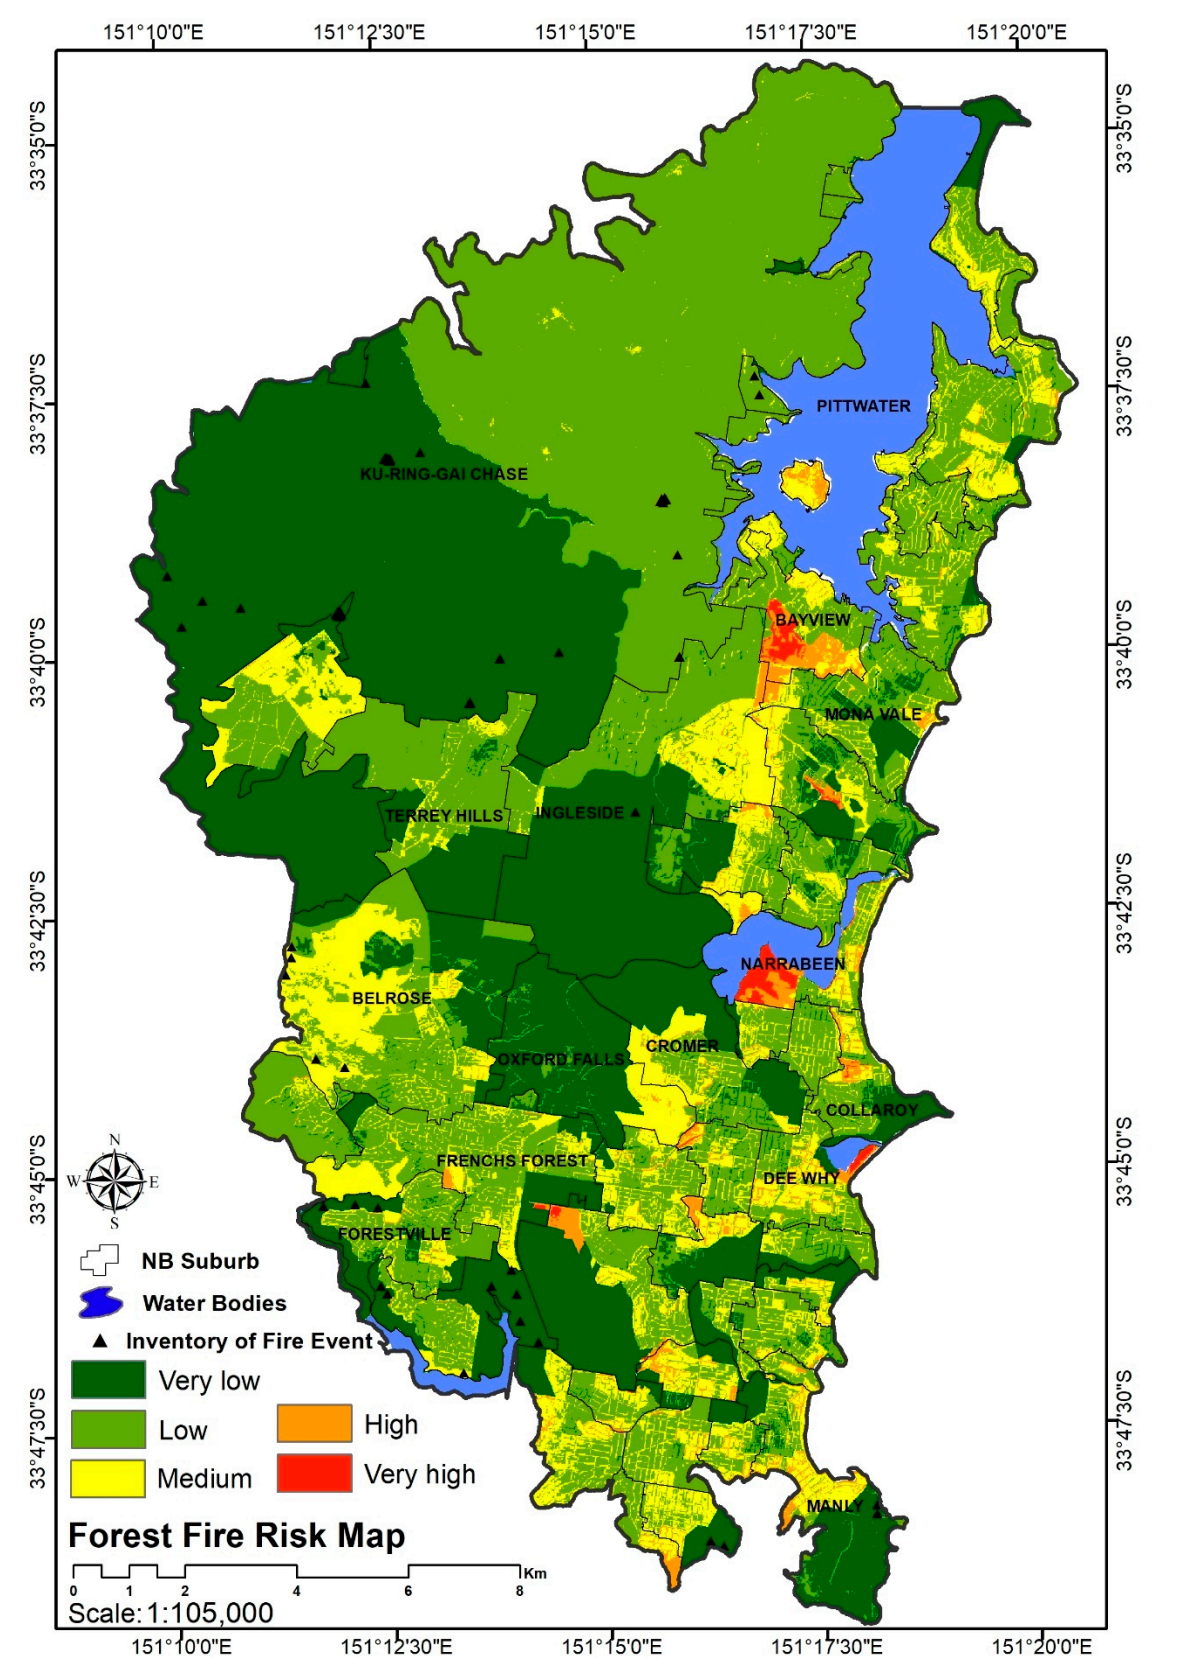
\includegraphics[width=0.4\linewidth]{frontmatter/imgs/Screenshot from 2023-11-28 11-07-47.png}
  \caption{Forest fire risk map}
  \label{fig:ffrpm}
\end{figure}



\subsection{Ant-miner algorithm}
A study conducted by \cite{ZHENG2020106772} mined decision rules using historical fire data and risk factor data from Chongqing, China. The authors stated risk factor data as a combination of the following parameters:
\begin{itemize}
    \item Meteorological data: wind speed, air temperature, relative humidity, accumulated precipitation, continued non-precipitation days;
    \item Land cover data: land cover type;
    \item human activity data: distance from nearest road and residential area.
\end{itemize}
An ant-miner algorithm was used to mine decision rules from the data and forecast the danger level of forest fire across the study region. A confusion matrix was also used in the study to assess the accuracy of the proposed model, which was then compared to existing models such as artificial neural networks, and support vector machines. 


The model was also compared to a risk prediction model based on meteorological data that calculated a \gls{ffdwi} according to China's national standard using five meteorological factors (wind speed, air temperature, relative humidity, accumulated precipitation, and continuous non-precipitation days). 


Another risk prediction model was based on the artificial neural network (ANN) technique, which employed the same risk elements (meteorological data, land cover data, and human activity data) to train a multilayer perceptron network for forecasting the risk level of forest fire. A support vector machine (SVM) was used and employed the same risk parameters as the proposed model to train a kernel-based classifier for predicting the risk level of forest fire.


The model's performance was compared using a confusion matrix. In terms of overall accuracy and Kappa coefficient, the ant-miner model surpassed the others.




The study acknowledged that the proposed model may lack generalisability across different geographical locations and may be unable to describe the risk distribution of forest fires as a specific mathematical function when multiple factors' joint probability distribution functions are considered.


\subsection{Fuzzy Inference}
The authors of \cite{LIN2018101} offer a novel approach for predicting and assessing forest fire risk using fuzzy inference (the process of applying fuzzy logic to create a mapping from a given input to an output \cite{KALOGIROU2009553}), and large data analysis. Figure \ref{fig:fuzzy_risk_prediction} explains visually the basic logic of the approach.


The project was built with a \gls{rwsn} in mind that is collecting continuous 24-hour meteorological data, and installed in a forest region in the Nanjing City region of China. Temperature, humidity, wind speed, rainfall, season, date, time, historical fire data, population density, fuel type, and road density are all input parameters.

\begin{figure}[h!]
 \centering
  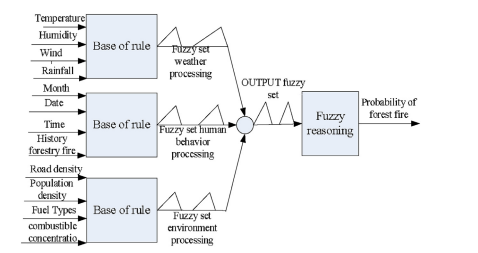
\includegraphics[width=0.7\linewidth]{frontmatter/imgs/fuzzy_prediction_model.PNG}
  \caption{Prediction of forest fire risk using a fuzzy reasoning algorithm \cite{LIN2018101}.}
  \label{fig:fuzzy_risk_prediction}
\end{figure}


The method generates the fire rating output by using triangular fuzzy numbers to reflect the uncertainty and ambiguity of the input parameters. The output fire rating is divided into five categories: low, moderate, high, very high, and extreme.
It was concluded that the system can accurately forecast possible fire danger and provide helpful information for forest fire prevention and management. Figure \ref{fig:prediction_graph_fuzzy} depicts fire probability given the oscillation of influencing factors. 

\begin{figure}[h!]
 \centering
  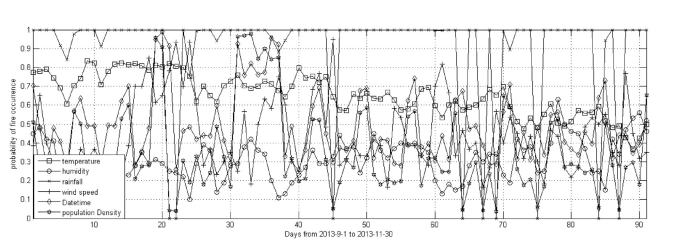
\includegraphics[width=1\linewidth]{frontmatter/imgs/p_ocurrencia_incendio.PNG}
  \caption{Meteorological data, datetime, and people density to predict the likelihood of a forest fire \cite{LIN2018101}.}
  \label{fig:prediction_graph_fuzzy}
\end{figure}



\subsection{Auto-sklearn}
An autonomous machine learning framework for forecasting the danger of forest fires based on meteorological data was proposed by \cite{Qu_2020}. This framework is capable of adapting to varied datasets and geographies. When it comes to binary unbalanced datasets, the machine learning techniques currently in use for forest fire prediction are not very compatible. 


The dataset used in the article comes from Montesinho Nature Park \cite{misc_forest_fires_162} and contains historical data about fire occurrences in the place. The framework optimises auto-sklearn, in terms of data preprocessing, parameter learning, and loss function.


The experimental findings demonstrated that the framework has strong geographic flexibility and performs better than other state-of-the-art machine learning techniques. Table \ref{sklearnpro} illustrates how Auto-Sklearn Pro performs better than other models when meta-learning is modified and a new bayesian optimisation index is included.




\begin{table}[h!]
\caption{Forest district classifier accuracy comparison}
\centering
\resizebox{\textwidth}{!}{%
\begin{tabular}{|c|c|c|c|}
\hline
\textbf{Forest District} & \textbf{Classifier} & \textbf{Accuracy (Overall)} & \textbf{Accuracy (Minority sample)} \\
\hline
District1 & AUTO-SKLEARN PRO & 87.3\% & 94.2\% \\
 & AUTO-SKLEARN & 86.4\% & 72.5\% \\
 & SVM & 84.6\% & 67.3\% \\
 & RandomForest & 75.5\% & 69.2\% \\
 & AUTO-SKLEARN PRO & 85.6\% & 90.4\% \\
\hline
District2 & AUTO-SKLEARN & 89.5\% & 74.3\% \\
 & SVM & 82.3\% & 63.2\% \\
 & RandomForest & 71.1\% & 73.0\% \\
 & AUTO-SKLEARN PRO & 82.4\% & 87.1\% \\
\hline
District3 & AUTO-SKLEARN & 85.3\% & 79.8\% \\
 & SVM & 73.1\% & 54.4\% \\
 & RandomForest & 69.5\% & 72.1\% \\
\hline
\end{tabular}%
}

\label{sklearnpro}
\end{table}


\subsection{DFP-MnBpAnn}
The authors behind \cite{TIENBUI2018104} proposed DFP-MnBpAnn, a new hybrid machine learning technique for spatial modelling of forest fire threat based on Artificial Neural Network (Ann) and a unique hybrid training algorithm of Differential Flower Pollination (DFP) and mini-match backpropagation (MnBp). 


Flower Pollination technique is a a nature-inspired, metaheuristic optimisation technique that mimics flower pollination. Solutions are viewed as flowers in FPA, and the process of identifying the optimum solution is analogous to pollination. 


Differential Evolution (DE), on the other hand, is a population-based optimisation technique that employs the evolutionary notion. It begins with a randomly generated population of solutions and improves them repeatedly using mutation, crossover, and selection procedures. 


The two algorithms are merged in such a way that they compliment each other in a hybrid training algorithm of DE and FPA \cite{Abdel-Basset2019}. 

\begin{figure}[h!]
 \centering
  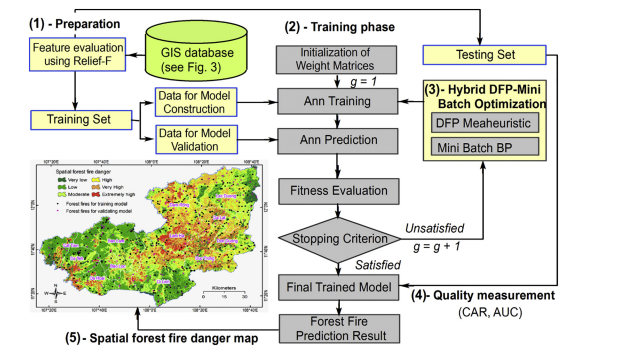
\includegraphics[width=1\linewidth]{frontmatter/imgs/hybrid_methodology.PNG}
  \caption{Methodology used with DFP-MnBpAnn\cite{LIN2018101}.}
  \label{fig:hybrid:dfpann}
\end{figure}

The factors influencing forest fire were slope, aspect, elevation (m), land use, NDVI, distance to road (m), distance to residential area (m), temperature (°C), wind speed (m/s), and rainfall (mm). They were generated from GIS data (see Figure \ref{fig:hybrid:dfpann} for a complete view of the proposed framework) to apply the suggested strategy to a tropical forest in Vietnam's Lam Dong province. 


The DFP-MnBpAnn model outperformed the other six approaches in terms of prediction accuracy (88.43\%) and AUC (0.94), highlighting its superiority and promise for large-scale forest fire threat mapping. The table \ref{table_dfp} presents the complete results of DFP-MnBpAnn's performance metrics against other models.


\begin{table}[h!]
\caption{DFP-MnBpAnn performance metrics against other prediction models \cite{TIENBUI2018104}}
    \centering
    \begin{tabular}{lccccccc}
        \hline
        \multirow{2}{*}{Phase} & \multirow{2}{*}{Model} & \multicolumn{6}{c}{Performance Metrics} \\
        \cline{3-8}
         & & CAR (\%) & AUC & TP & FP & FN & TN \\
        \hline
        \multirow{6}{*}{Training} & DFP-MnBpAnn & 87.30 & 0.91 & 0.94 & 0.20 & 0.06 & 0.80 \\
         & PSO-NF & 89.30 & 0.93 & 0.96 & 0.17 & 0.04 & 0.83 \\
         & RF & 86.40 & 0.91 & 0.91 & 0.19 & 0.09 & 0.81 \\
         & SVM & 86.20 & 0.89 & 0.92 & 0.19 & 0.08 & 0.81 \\
         & LSSVM & 86.24 & 0.89 & 0.90 & 0.18 & 0.10 & 0.82 \\
         & BpAnn & 89.02 & 0.94 & 0.93 & 0.15 & 0.07 & 0.85 \\
        \hline
        \multirow{6}{*}{Testing} & DFP-MnBpAnn & 89.20 & 0.94 & 0.94 & 0.15 & 0.06 & 0.85 \\
         & PSO-NF & 85.80 & 0.92 & 0.92 & 0.20 & 0.08 & 0.80 \\
         & RF & 85.20 & 0.91 & 0.90 & 0.19 & 0.10 & 0.81 \\
         & SVM & 84.90 & 0.88 & 0.88 & 0.19 & 0.12 & 0.81 \\
         & LSSVM & 86.42 & 0.88 & 0.92 & 0.19 & 0.08 & 0.81 \\
         & BpAnn & 85.03 & 0.89 & 0.91 & 0.21 & 0.09 & 0.79 \\
        \hline
    \end{tabular}
    \label{table_dfp}
\end{table}


\section{Methodologies for data aggregation, fusion, and enhancement}
\subsection{Data aggregation}
The process of merging information from several sources into a single dataset is known as data aggregation. These sources may consist of databases, sensor networks, or other types of data repositories containing Weather, location, and historical fire event data \cite{Cai2019}. Data aggregation can be split into two key-categories \cite{papvco2021fusion}:
\begin{itemize}
    \item Temporal aggregation: Combining data across predetermined time frames. Finding trends linked to fire seasonality, such as daily meteorological data that may be combined to produce monthly or seasonal averages \cite{papvco2021fusion}.
    \item Spatial aggregation: Combining data across geographic regions. This can aid in comprehending how fire risk elements are distributed spatially \cite{papvco2021fusion}.
\end{itemize}

\subsection{Data fusion}
\label{data_fusion}
Data fusion refers to the need to combine information obtained from many sources (sensors, databases, information gathered by people, apis) in order to present complementary interpretations of the same phenomenon. It provides more exact results than those obtained by using a single dataset, eliminating ambiguity and redundancy. \cite{CHATZICHRISTOS2022341, LACROIX200375}

Figure \ref{fig:meth:data_fusion} describes visually two data fusion techniques that will be utilised. The following list explains each one:
\begin{itemize}
    \item Decision-Level fusion: In this technique, characteristics are extracted from the data and one or more intermediate analyses are carried out until an appropriate result for the problem is achieved \cite{articleDataFusion}.
    \item Feature-level fusion: This technique involves collecting features from each data source and then merging them \cite{articleDataFusion}.
\end{itemize}

\begin{figure}[h!]
 \centering
  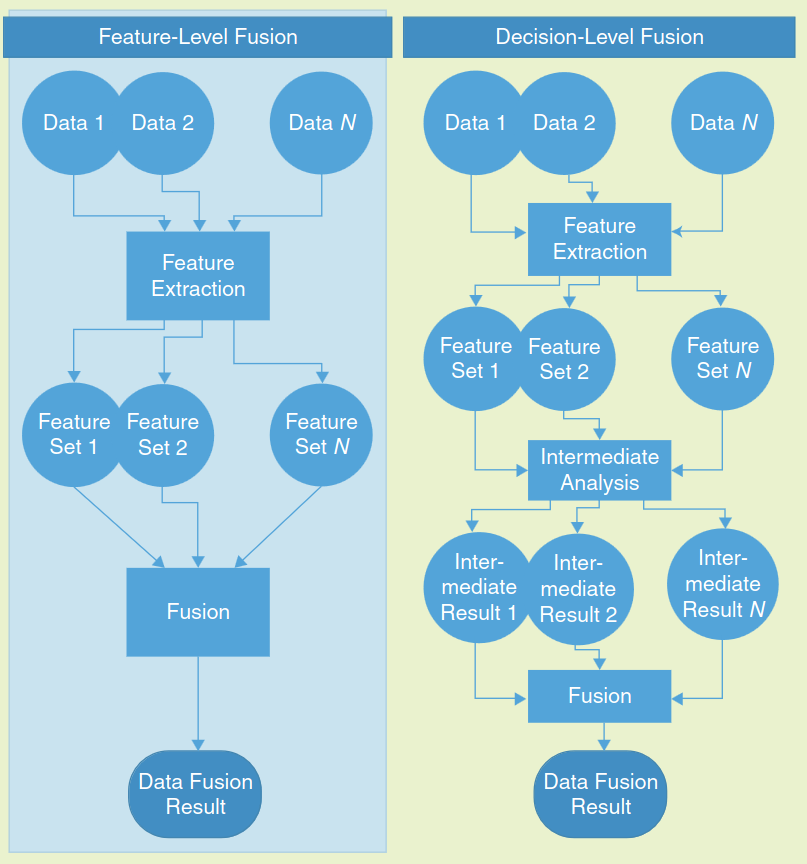
\includegraphics[height=0.7\linewidth]{frontmatter/imgs/ffdf2.png}
  \caption{Methodologies for Data fusion \cite{articleDataFusion}.}
  \label{fig:meth:data_fusion}
\end{figure}

\subsection{Data enhancement} 
The process of changing, converting, or adding to data in order to make it better and easier to use is known as data enhancement \cite{clickworker2021}. 
It can be achieved by using multiple paths such as:
\begin{itemize}
    \item Data Enrichment: Using numerous third-party data to supplement the original data \cite{mparticle_data_enrichment}.
    \item Synthetic Data Generation: Created artificially without utilising the original dataset \cite{awan2023complete_guide_data_augmentation}.
\end{itemize}



\section{Tools for data visualization}

\subsection{Seaborn}
\label{dv_seabon}
Seaborn is a high-level interface for creating visually appealing statistical visuals and is developed on top of Matplotlib, which is a charting toolkit and allows the creation of all kinds of plots and charts \cite{seaborn}\cite{matplotlib}.

\subsection{Folium}
Folium is a Python wrapper for Leaflet.js map tool. It helps in spatial data visualisation \cite{folium}.

\subsection{GeoPlot}
It is based on Matplotlib and GeoPandas. Geoplot offers a high-level mapping creation interface. GeoPandas is a library extension for Pandas that facilitates mapping and has geographic functions. It manages and produces maps using geospatial data \cite{geoplot, geopandas, matplotlib}.

\subsection{Plotly}
\label{dv_plotly}
Plotly is a robust and interactive charting library. It works with many different kinds of charts and is helpful for making interactive visualisations. \cite{plotly}.

\subsection{Rasterio}
Rasterio is used to read and write geographic raster data, such as satellite images. \cite{rasterio}.

\subsection{Pydeck}
Pydeck is a WebGL-powered, high-layer framework that is used to create dynamic maps covering sizable regions \cite{pydeck}.

\subsection{Rasterstats}
Geospatial raster datasets may be summarised using rasterstats based on vector geometry. It is also used to compute statistics within certain regions \cite{rasterstats}.

\subsection{Fiona}
The goal of Fiona is to simplify the reading and writing of geographic data files. It makes dealing with vector data easier and is based on GDAL which is a potent open-source library for reading and writing geographic data formats in both raster and vector forms. \cite{fiona, gdal}.


\section{State-of-the-art conclusion}

Throughout this chapter, various methodologies for predicting occurrence, susceptibility, and risk of fires have been discussed. As this problem is highly dependent on the data that can be obtained from multiple sources, some methodologies like \cite{sadatrazavi2022predicting} and \cite{bountzouklis2023predicting} can be discarded, as they lack generalisation and are only suited for one purpose. \cite{sadatrazavi2022predicting} carried out a study between the susceptibility of two types of forests and concluded the factors that influence the ignition of fire in each type, and \cite{bountzouklis2023predicting} showed that naturally ignited fire is the easiest one to predict.


The paper conducted by \cite{10085661} should also not be taken as guidance. Although the employed logistic regression obtained an accuracy value of 93.75\%, its approach is very narrow as only three variables were used.


For an initial prototyping phase, random forests seem to be a good candidate, as shown in \cite{abid2020predicting} and \cite{9726029}. The authors of \cite{abid2020predicting} used a decision tree classifier and obtained an accuracy of 82.92\%. While \cite{9726029} didn't explicitly mention the accuracy metric, its random forest classifier obtained a regression score of 97.99\%.


ANN is a great option overall for fire occurrence prediction. \cite{SAYAD2019130} compared the accuracy between ANN and SVM, while these two had very high accuracy ratings. ANN got the upper hand with 98.32\% against SVM's 97.42\%. Once the prototyping phase with random forests has been completed, ANN could be the de facto option for forest fire occurrence prediction.


The study carried out by \cite{POURGHASEMI2020109321} demonstrated that for fire susceptibility, boosted regression trees are better than GLM and MDA. Fire susceptibility can be inherently connected to risk prediction. It can be a step in the prediction of risk. Therefore, it is not necessary to provide a specific solution for susceptibility like the authors of \cite{POURGHASEMI2020109321} did.


Most of the studies conducted in the field of risk prediction employed a hybrid approach. These approaches lack generalisation, as seen in \cite{ZHENG2020106772}, and are much harder to implement.


The authors of \cite{TIENBUI2018104} used a novel approach to map the forest fire ignition risk. This method used a hybrid model and yielded a high AUC score of 0.94. Although this method uses a hybrid approach, the underlying model is still an ANN. Emphasising once again the usefulness of an ANN approach for both occurrence and risk prediction.


The study conducted by \cite{Qu_2020} created a framework with auto-sklearn capable of adapting itself to multiple geographical locations. This is a very important feature for risk prediction, and this approach can also be taken into consideration as it uses an easy to obtain dataset, so result metrics can be easily compared. This study had an accuracy of 87.3\%.


The tools for data visualisation are also dependable on the obtained data. But tools like plotly (\ref{dv_plotly}) and seaborn (\ref{dv_seabon}) will always be used due to their generic capabilities. These libraries serve the purpose of plotting data.


The methodologies for data aggregation, fusion, and enhancement presented previously will also be used, as they represent standard procedures for machine learning data preparation.



\cleardoublepage

\glsresetall




%\chapter{Solution Proposal}
\label{sec:solution_proposal}

This chapter will define the problem, establish how success will be evaluated, define the methodology for developing the solution, and present the associated risks.

\section{Problem definition}


The challenge is to design and develop a comprehensive system that can effectively process, validate, and aggregate voluntary contributions supported by various types of data. This system would need to be able to classify the severity of forest fire events based on aggregated data.

Moreover, it would need to identify the geolocation and track the temporal evolution of a wildfire event. Providing properly organised and validated information is crucial, as it can help increase knowledge about the event, facilitate real-time decision-making, and potentially save lives and resources.


Finally, the system would need a set of plotting tools to aid in information gathering and posterior analysis.



Figure \ref{fig:mockup_presentation} shows in rudimentary way, multiple geographic location that don't have correlation to each other. Each tile represents a different biome, and each one is named after a letter. Fire risk is composed of four distinct categories, red which is associated with extreme risk of fire, orange is high risk, yellow is moderate risk, and green is low risk of fire.
Tile C is on the worst-risk. There are several active fire fronts, and it is windy. 


Tile A has high risk and has a forest near a rural area, this may have enhanced fire ignition due to human activities. Tile B is near a town, but since it isn't windy or very hot, it has a moderate risk of fire. Tile D is the least likely to catch on fire, it is raining and the weather is cold. It has a risk score of green signalling a low risk of fire.


This imaginary exercise can be converted into the real world, because it entangles the problem at its core. Create a fire risk and occurrence analysis with multiple sources of data and then show it in a easy manner.


The tiles would be geographical areas, and risk would be associated with it given each region's fire influencing factors.


In essence, the goal is to create a comprehensive system that can handle a wide range of data types, make sense of this data, and provide actionable insights about forest fire events.


\begin{figure}[h!]
 \centering
  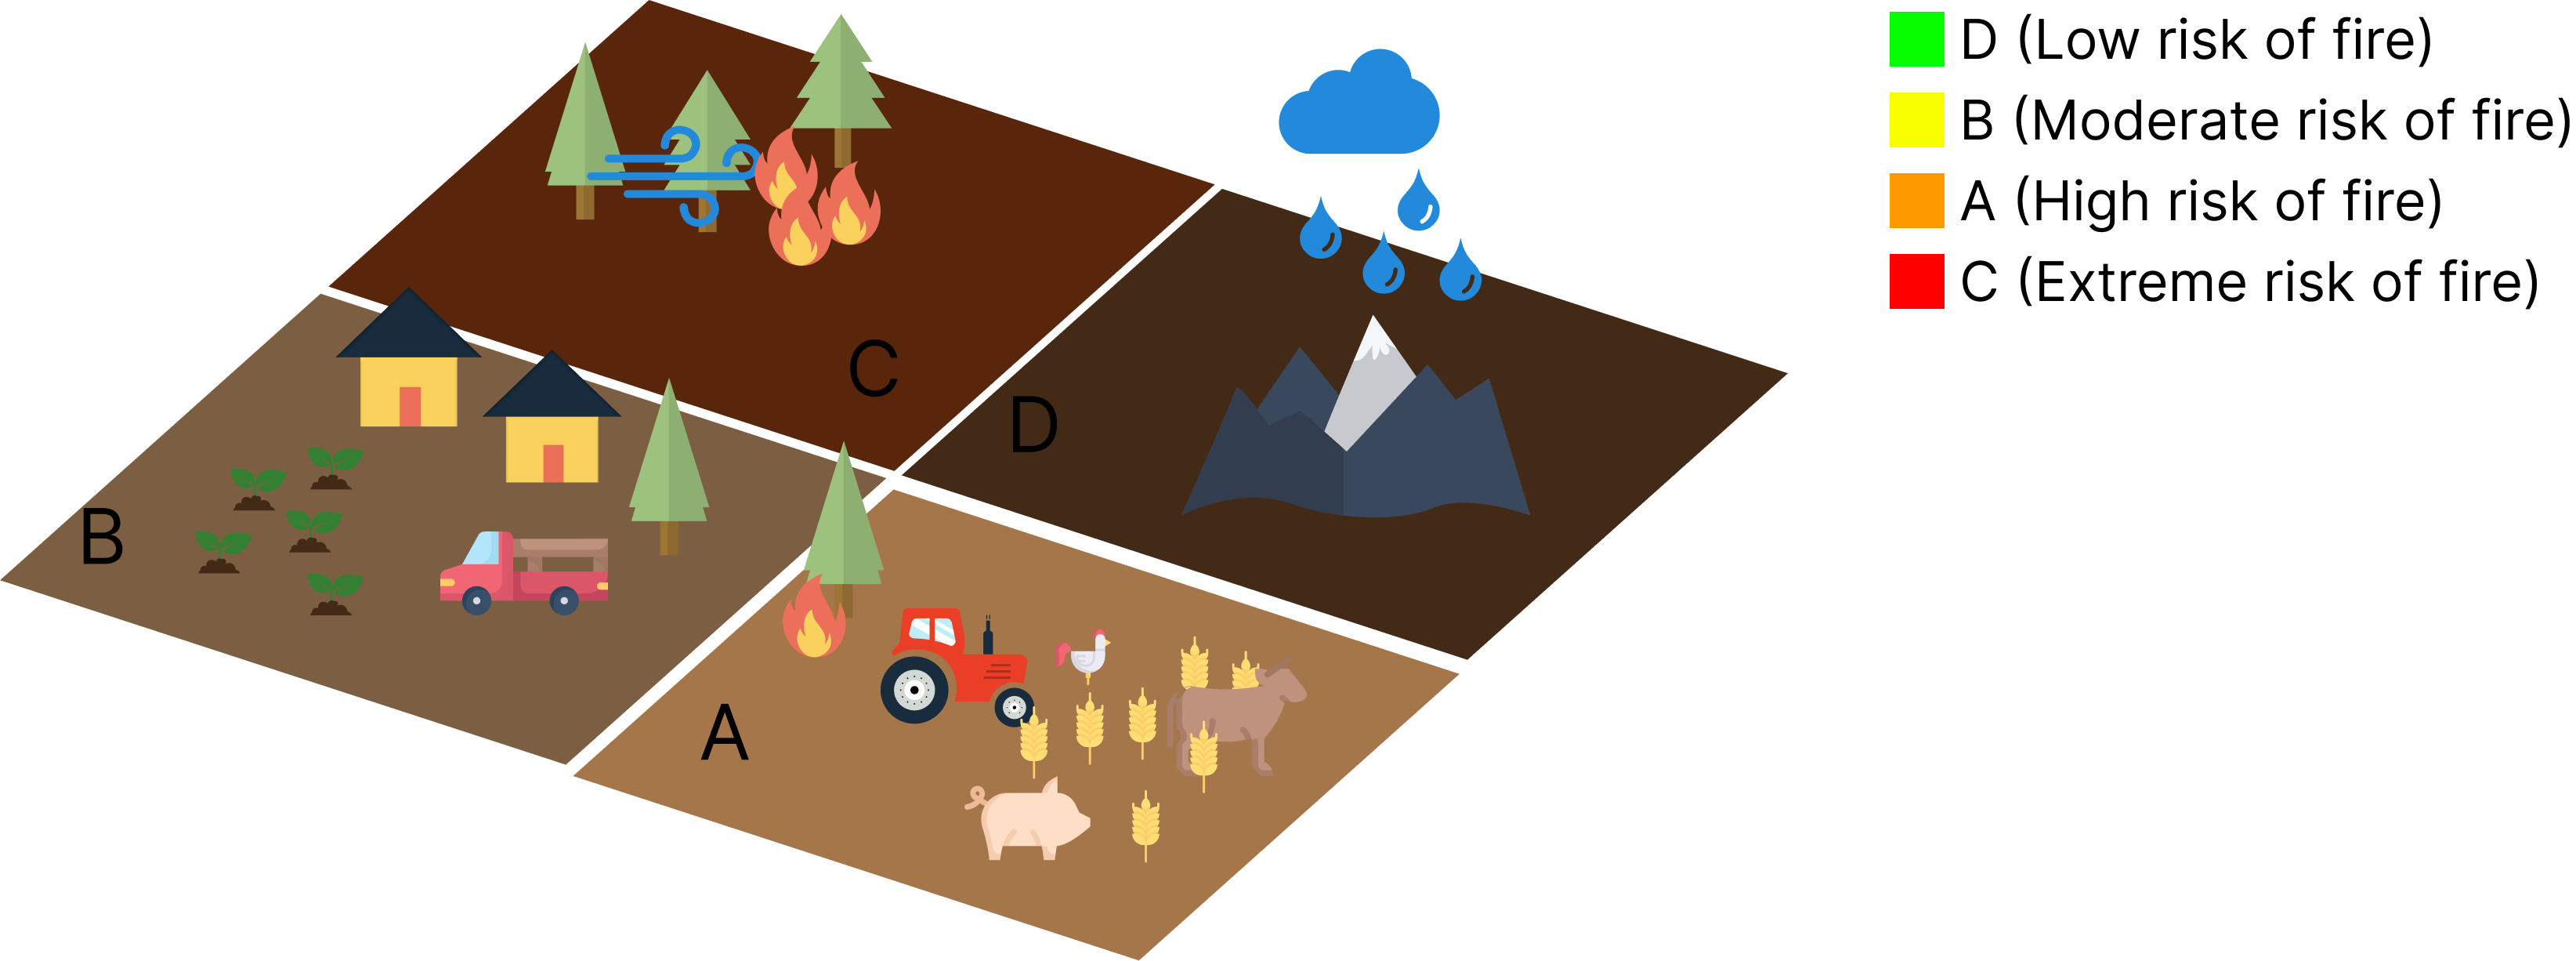
\includegraphics[width=1.0\linewidth]{frontmatter/imgs/Group 1.png}
  \caption{Tiles depicting geographical areas and forest fire risk}
  \label{fig:mockup_presentation}
\end{figure}

\section{Proposed Methodology}
The methodology section will cover the steps for carrying out the solution. Firstly, data is collected from various sources to create a data pipeline. This is followed by the step of merging the data according to its features. The fusion can be done recursively until there is satisfaction with the information obtained.


The data will be combined with other external sources, and depending on the scarcity of the data, it may be necessary to generate synthetic data. Once the data has been cleaned, it will be placed in a database.


The models will use the database to obtain classification results. The results will focus on risk, susceptibility, and fire occurrence. Finally, with the help of data visualisation tools, the findings will be displayed.

\subsection{Data Pipeline} 
Data pipeline is the process of extracting, transforming, and loading data from diverse sources, such as volunteer contributions, geographical data, and meteorological data. The following steps comprise the data pipeline:

\subsubsection{Data extraction}
Data is gathered from a variety of sources, including websites, APIs, and databases.

\subsubsection{Data transformation}
Following extraction, the data is cleaned (duplicates are removed and missing values are handled), normalized (ensuring that is in a consistent format), and enriched. 

\subsubsection{Data loading}
The transformed data is then loaded into an appropriate data storage system, such as a database. This enables efficient searching and retrieval of data when it is required for analysis.

\subsection{Data Fusion}
Data fusion can happen at the data transformation step. At this level, decision-level and feature-level fusion will occur (see \ref{data_fusion} for a more detailed explanation of each one).

\subsection{Data enhancement}
Data enhancement follows the fusion step. At this level, data can be enriched with external sources or generated.


\subsection{Classification Models}
Experiments will be conducted on data with multiple machine learning models to convey the ones with better metrics and performance and highlight the most useful features in forest fire event classification. For fire occurrence, Random Forest and SVM are strong candidates for a first approach. These two models are easy to implement and highlighted high results in \cite{9726029} and \cite{SAYAD2019130}. For fire risk, an ANN model is the strongest candidate, as shown in \cite{rs13132513}.

\subsection{Data Visualisation}
Data visualisation will enable the plotting and presentation of forest fire severity classification results, as well as the display of aggregated and validated information.


\subsection{Outcome}
The project's output would be the information derived from the classification models. If in a given area or given some meteorological indices, the system will determine the likelihood of fire (fire or no fire) and the associated risk (low, moderate, high, or extreme). This information will be presented using data visualisation tools.


\section{Planning and organisation}
Figure \ref{fig:gantt_first} exhibits the time taken for each step in the first semester. It has a comparison between the time expected for each task and the actual time taken to complete it. The comprising steps in the first Gantt chart are:
\begin{enumerate}
    \item Learn Key Concepts - Forest Fire Management, Issues, Decision Support systems;
    \item Learn Key Concepts - Machine learning applied to forest fire, Mathematical models, and Influencing factors;
    \item Learn models used to classify Forest Fire;
    \item Research data visualisation tools and libraries;
    \item Study of the problem;
    \item Define the solution, objectives, success criteria, risks and methodology;
    \item Write document.
\end{enumerate}


Figure \ref{fig:gantt_second} shows the proposed Gantt chart for the second semester. The following list will explain each step in figure \ref{fig:gantt_second}:

\begin{enumerate}
    \item Collect data from multiple sources: The first step involves the gathering of multiple data sources;
    \item Extract, Transform, and Load Data: Apply extract, transform, and load techniques to the gathered data. In this step, the data pipeline is created.
    \item Fusion techniques on data: This step undertakes the fusion methodologies inside the pipeline;
    \item Conduct forest fire event classification with RF and ANN models: Random forest and ANN have been chosen as the first candidates to tackle the problem of forest fire occurrence and risk;
    \item Utilise fused and classification outputs to visualise the information: This is regarded as the last step in the system's implementation. The findings discovered in the previous steps are now interpretable information ready to be used in a decision-support system;
    \item Assemble the scientific paper: Besides the thesis, this project should result in a scientific paper;
    \item Write document: The last step is the completion of the thesis document.
\end{enumerate}

\begin{figure}[h!]
 \centering
  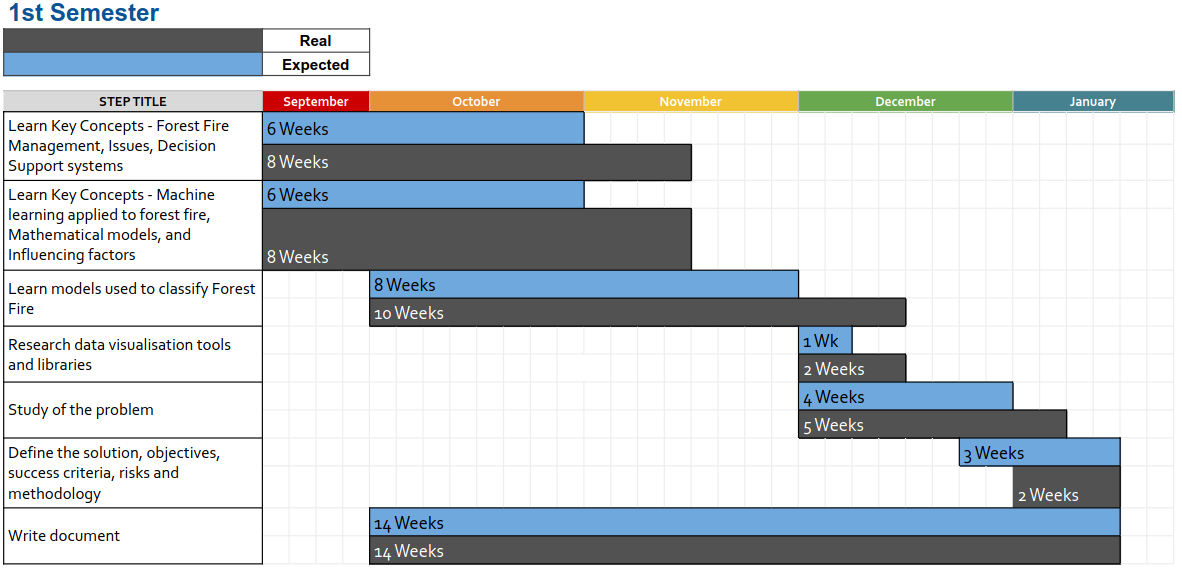
\includegraphics[width=1.0\linewidth]{frontmatter/imgs/g1.png}
  \caption{Gantt chart for first semester}
  \label{fig:gantt_first}
\end{figure}

\begin{figure}[h!]
 \centering
  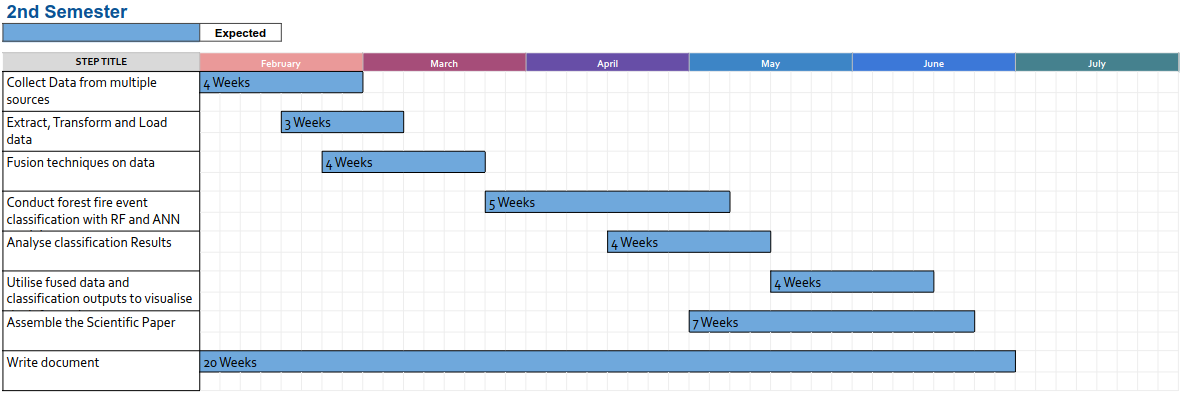
\includegraphics[width=1.0\linewidth]{frontmatter/imgs/g2.png}
  \caption{Proposed gantt chart for the second semester}
  \label{fig:gantt_second}
\end{figure}


\section{Risk analysis}
In this section, the potential risk that may affect the success of the approach is identified, and mitigation and impact plans for the risk are proposed. A qualitative probability and impact level were also assigned using the following scales: low, medium, and high. Table \ref{risk_du} outlines the only identified risk.

\begin{table}[h!]
\caption{Risk - Data unavailability}
\label{risk_du}
\begin{tabular}{|p{2cm}|p{12cm}|}
\hline
Risk            & Data unavailability \\ \hline
Description     & Due to technological challenges, privacy limitations, or other factors, some data sources may not be available. \\ \hline
Mitigation Plan & To provide data redundancy and variety, many data sources are employed.  \\ \hline
Impact Plan     & Identify alternative data sources. Generate data. Adapt the prediction model to work effectively with the available data. Adapt the experiment to the available data. \\ \hline
Probability     & High \\ \hline
Impact          & High \\ \hline
\end{tabular}
\end{table}


\section{Success Evaluation Criteria}
The success of the project can be measured in two dimensions: the realisation of the proposed objectives and how closely the outcomes resemble reality. That is, whether the system is able to assess whether there is a likelihood of fire or not. Also, regarding success outcomes, data visualisation should play a key role in showing findings in a clean manner. Therefore, the following steps must be considered when evaluating the success of the outcomes:

\subsection{Classification performance}
The classification model's accuracy, precision, recall, F1-score, and AUC will be evaluated. The models will be also compared to other classification results and sources on historical data. 
Different machine learning algorithms' performance will be examined, and feature selection approaches will be utilised to discover the best model and the most significant characteristics for the classification problem.


\subsection{Visualization effectiveness}
The visualisation should be simple, and easy to follow. This can be achieved by following design guidelines and making comparisons with other data visualisation interfaces. 



\chapter{Implementation}
\label{sec:implementation}

\section{Data Sources}

\subsection{Historical record of fires from 1980 to 2015 in mainland Portugal \cite{centraldedados_incendios_website}\cite{centraldedados_incendios} \cite{icnf2024}}

//describe dataset here, how many entries?
\label{historical_sites_no_coords}

\begin{table}[h!]
\caption{Field description of Historical fires from 1980 to 2015}
\label{forest_inventory}
\centering
\small
\begin{tabular}{|c|p{7.5cm}|} % Adjust width as necessary
\hline
\textbf{Variable} & \textbf{Description}\\
\hline
ano  & Year of fire occurrence \\
\hline
codigo\_sgif & Unique identifier for the fire occurrence \\
\hline
tipo  & Kind of wildfire. The available options are: forest, slash-and-burn, false alarm, and agricultural.\\
\hline
distrito  & District of fire occurrence. \\
\hline
concelho  & Municipality of fire occurrence. \\
\hline
freguesia  & Parish of fire occurrence.\\
\hline
local  & Location of fire occurrence. \\
\hline
ine  & Not described or explained anywhere. \\
\hline
x | y  & Wildfire location. \\
\hline
data\_alerta  & Wildfire warning date. \\
\hline
hora\_alerta  & Wildfire warning hour. \\
\hline
data\_extincao & Wildfire complete extinguishment date. \\
\hline
hora\_extincao & Hour of wildfire complete extinguishment. \\
\hline
data\_primeira\_intervencao & Date of first fire intervention \\
\hline
hora\_primeira\_intervencao & Hour of first fire intervention \\
\hline
fonte\_alerta & Authority or group of people who reported the fire first. \\
\hline
nut & A Unique identifier for a given nomenclature of territorial units for statistics. \\
\hline
area\_povoamento & Burnt settlement area. \\
\hline
area\_mato & Burnt bush area.  \\
\hline
area\_agricola & Burnt agricultural area. \\
\hline
area\_pov\_mato & Sum of burned area from the burnt settlement area and burnt agricultural area.\\
\hline
area\_total & Total burnt area. \\
\hline
reacendimento & Describes if a given fire is a re-ignition from a previous wildfire. \\
\hline
queimada & Identifies if a fire is a slash-and-burn. \\
\hline
falso\_alarme & Identifies if it is a false alarm. \\
\hline
fogacho & Identifies if it is a specific type of fire named a blaze. \\
\hline
incendio & Identifies if it is a fire. \\
\hline
causa & Numerical identifier for the fire cause. \\
\hline
tipo\_causa & Description of fire cause. The available options are unknown, deliberate, natural, negligent fire, and undefined. \\
\hline
\end{tabular}
\end{table}


\subsection{Historical record of fires from 2013 to 2023 in mainland Portugal \cite{icnf2024}}
\label{dataset_icnf2013_2023}

Data retrieved from the API \href{https://fogos.icnf.pt/localizador/webserviceocorrencias.asp?ano=YEAR}{endpoint}.
//describe dataset here, how many entries?


\begin{table}[h!]
\caption{Field description of Historical fires from 2013 to 2024}
\label{forest_inventory}
\centering
\small
\begin{tabular}{|c|p{7.5cm}|} % Adjust width as necessary
\hline
\textbf{Variable} & \textbf{Description}\\
\hline
CODIGO id  & Unique identifier for the fire occurrence \\
\hline
DISTRITO  & District of fire occurrence. \\
\hline
TIPO  & Kind of wildfire. The available options are: forest and agricultural fire.\\
\hline
ANO  & Year of fire occurrence \\
\hline
AREAPOV & Burnt settlement area. \\
\hline
AREAMATO & Burnt bush area.  \\
\hline
AREAAGRIC & Burnt agricultural area. \\
\hline
AREATOTAL & Total burnt area. \\
\hline
REACENDIMENTOS & Boolean value for reignition. \\
\hline
FOGACHO & Boolean value for small fire. \\
\hline
NCCO & Non specified identifier. \\
\hline
NOMECCO & Not described or explained anywhere. \\
\hline
DATAALERTA & Wildfire warning date. \\
\hline
HORAALERTA & Wildfire warning hour. \\
\hline
LOCAL & Location of fire occurrence \\
\hline
CONCELHO & Municipality of fire occurrence. \\
\hline
FREGUESIA & Parish of fire occurrence\\
\hline
FONTEALERTA & Authority or group of people who reported the fire first. \\
\hline
INE & Not described or explained anywhere. \\
\hline
X | Y & Wildfire location. \\
\hline
DIA & Day of the fire occurrence. \\
\hline
MES & Month of fire occurrence. \\
\hline
HORA & Fire hour of occurrence. \\
\hline
OPERADOR & Not described or explained anywhere. \\
\hline
PERIMETRO & Not described or explained anywhere. \\
\hline
APS & Not described or explained anywhere. \\
\hline
CAUSA & Numerical identifier for the fire cause. \\
\hline
TIPOCAUSA & Description of fire cause. The available options differ from year to year. \\

distrito  & District of fire occurrence. \\
\hline


local  & Local of fire occurrence \\
\hline


data\_alerta  & Wildfire warning date. \\
\hline
hora\_alerta  & Wildfire warning hour. \\
\hline
data\_extincao & Wildfire complete extinguishment date. \\
\hline
hora\_extincao & Hour of wildfire complete extinguishment. \\
\hline
data\_primeira\_intervencao & Date of first fire intervention \\
\hline
hora\_primeira\_intervencao & Hour of first fire intervention \\
\hline
fonte\_alerta & Authority or group of people who reported the fire first. \\
\hline
nut & A Unique identifier for a given nomenclature of territorial units for statistics. \\
\hline



area\_pov\_mato & Sum of burned area from the burnt settlement area and burnt agricultural area.\\
\hline

reacendimento & Describes if a given fire is a re-ignition from a previous wildfire. \\
\hline
queimada & Identifies if a fire is a slash-and-burn. \\
\hline
falso\_alarme & Identifies if a false alarm. \\
\hline
fogacho & Identifies if it is a specific type of fire named a blaze. \\
\hline
incendio & Identifies if it is a fire. \\
\hline
causa & Numerical identifier for a fire cause. \\
\hline
tipo\_causa & Description of fire cause. The available options are unknown, deliberate, natural, negligent fire, and undefined. \\
\hline
\end{tabular}
\end{table}



\subsection{Study area}
MUDAR
The study area is located in western Sichuan, southwest China, between 26 05 00 N to 34 20 00 N and 97 22 00 E to 104 07 00 E, with a
total area of about 300,423 km2
(Fig. 2a). Belonging to the southeastern edge of the Qinghai-Tibet
Plateau, the area is characterized by complex topography, with a low
evaluation in the south region (around 1500 m a.s.l.) to a high evalua-
tion in the north region (around 4500 m a.s.l.). Wildfires only seldom
occur above 4000 m a.s.l., so we limited our study area to the region
below 4000 m a.s.l.
The climate in the study area varies with altitude and ranges from
alpine in the northern area to the subtropical semi-humid climate in the
southern mountainous area. The alpine climate in the northwestern
region faces water scarcity (annual total precipitation of 500–900 mm


\subsection{Open-meteo hourly weather variables \cite{Zippenfenig_Open-Meteo}}
Historical Weather \cite{Zippenfenig_Open-Meteo} from \cite{Hersbach_ERA5}, \cite{Munoz_ERA5_LAND} and \cite{Schimanke_CERRA}
\label{open_meteo}
\begin{table}[h!]
\caption{Hourly weather variables from Open-meteo}
\centering
\small
\begin{tabular}{|c|c|p{10cm}|} % Adjust width as necessary
\hline
\textbf{Variable} & \textbf{Unit} & \textbf{Description}\\
\hline
Temperature & °C & Air temperature 2 metres above ground. \\
\hline
Relative Humidity & \% & Relative humidity 2 metres above ground. \\
\hline
Dew & °C & Dew point 2 metres above ground. \\
\hline
Apparent Temperature & °C & Apparent temperature is the 
result of a wind chill factor, relative humidity, and solar radiation. \\
\hline
Pressure & hPa & Atmospheric air pressure reduced to mean sea level. \\
\hline
Surface Pressure & hPa & Surface pressure reduced to mean sea level. \\
\hline
Precipitation & mm & Sum of preceding hour precipitation including rain, showers, and snow. \\
\hline
Rain & mm & Preceding hour of liquid precipitation. \\
\hline
Snowfall & cm & Preceding hour of snowfall amount. \\
\hline
Cloud cover low & \% & Fog and low level clouds up to an altitude of 2 kilometres. \\
\hline
Cloud cover mid & \% & Clouds floating at a medium level with altitudes ranging from 2 kilometres to six kilometres. \\
\hline
Cloud cover high & \% & Clouds floating at an altitude of 6 kilometres. \\
\hline
Shortwave radiation & $W/m^2$ & Shortwave solar radiation.  \\
\hline
Direct radiation & $W/m^2$ & Direct solar radiation. \\
\hline
Direct normal irradiance & $W/m^2$ & Direct solar irradiance.  \\
\hline
Diffuse radiation & $W/m^2$ & Diffuse solar radiation.  \\
\hline
Global tilted irradiance & $W/m^2$ & Total radiation received on a tilted pane.  \\
\hline
Sunshine duration & Seconds & Duration of sunshine in seconds.  \\
\hline
Wind speed at 10m & km/h & Speed of the wind, 10 metres above ground.  \\
\hline
Wind speed at 100m & km/h & Speed of the wind, 100 metres above ground.  \\
\hline
Wind direction at 10m & ° & Wind direction at 10 metres above ground.  \\
\hline
Wind direction at 100m & ° & Wind direction at 100 metres above ground.  \\
\hline
Wind gusts & km/h & Wind gusts at 10 metres above ground.  \\
\hline
Evapotranspiration & mm & Evapotranspiration value for the required irrigation for plants calculated from temperature, wind speed, humidity, and solar radiation. \\
\hline
Weather code & WMO code & Numeric codes for weather conditions.  \\
\hline
Snow depth & meters & The depth of snow on the ground.  \\
\hline
Vapour pressure deficit & kPa & Vapour pressure deficit in kilopascal.\\
\hline
Soil temperature & °C & Average soil temperature ranging from 0 to 7cm, 7 to 28cm, 28 to 100cm, and 100 to 255cm below ground.\\
\hline
Soil moisture & $m^3/m^3$ & Average soil moisture ranging from 0 to 7cm, 7 to 28cm, 28 to 100cm, and 100 to 255cm depths.\\
\hline
\end{tabular}
\end{table}

\subsection{Fire danger indices historical data from the Copernicus Emergency Management Service \cite{CopernicusCDS2019}}
The dataset "Fire danger indices historical data from the Copernicus Emergency Management Service" \cite{CopernicusCDS2019} provided by ECMWF, contains full historical reconstruction of weather conditions suitable for the origin, spread, and sustainability of natural occurring fires. 

It embodies fire danger indices from three distinct models created in Canada, United States and Australia. The fire danger indices are obtained from historical simulations and weather forecast provided by the dataset ECMWF ERA5 reanalysis. 

The available data starts from January 1940 and it extends all the way through 2023, but the data records are regularly extended with time as ERA5 forcing data becomes available. The variables contained in the dataset are expressed in the table \ref{copernicus_danger_indices}.


\begin{table}[h!]

\caption{Fire danger indices from historical data}
\label{copernicus_danger_indices}
\centering
\small
\begin{tabular}{|c|c|p{7.5cm}|} % Adjust width as necessary
\hline
\textbf{Variable} & \textbf{Unit} & \textbf{Description}\\
\hline
Build-up index & Dimensionless & Weighted combination of the Duff moisture code and Drought code. \\
\hline
Burning index & Dimensionless & Measure that explains how difficult it is to control a fire. \\
\hline
Danger rating & Dimensionless & Equivalent to the FWI but with class level definitions of very low, low, medium, high, very high and extreme. \\
\hline
Drought code & Dimensionless & Component representing fuel availability, and the influence of recent temperatures and rainfall events on fuel availability. \\
\hline
Duff moisture code & Dimensionless & Moisture content in loosely-compacted organic layers of moderate depth. Duff moisture code fuels are affected by rain, temperature and relative humidity. \\
\hline
Energy release component & $J/m^2$ & Available energy within the burning front at the head of a fire. \\
\hline
Fine fuel moisture code & Dimensionless &  Moisture content in litter. Representative of the top litter layer less than 1-2 cm deep. \\
\hline
Fire daily severity index & Dimensionless &  A numerical assessment of the difficulty of controlling flames. \\
\hline
Fire danger index & Dimensionless &  Metric that hold the chances of a fire starting. \\
\hline
Fire weather index & Dimensionless &  Combination of Initial spread index and Build-up index. Numerical rating of the potential fire intensity. \\
\hline
Ignition component & \% &  Probability of a firebrand that will require suppression action. \\
\hline
Keetch-Byram drought index & Dimensionless &  The total impact of evapotranspiration and precipitation in causing cumulative moisture shortage in deep duff and higher soil layers. \\
\hline
Spread component & Dimensionless &  Measure of the spead at which a headfire would spread. \\
\hline
\end{tabular}
\end{table}



\subsection{Forest Inventory 2015 \cite{uva2021forestry,https://doi.org/10.15468/dl.zwfmbt}}
Forest Inventory 2015 contains 579422 occurrences of forest inventory for mainland Portugal. The data was gathered using aerial images and ground surveys that covered mainland Portugal. 
//describe dataset here


\begin{table}[h!]
\caption{Forest Inventory 2015}
\label{forest_inventory}
\centering
\small
\begin{tabular}{|c|p{7.5cm}|} % Adjust width as necessary
\hline
\textbf{Variable} & \textbf{Description}\\
\hline
gbifID | datasetKey | ocurrenceID  & Identifiers for the occurrence of trees and the dataset. \\
\hline
kingdom & Kingdom classification of a given Tree. \\
\hline
phylum & Phylum classification of a given Tree. \\
\hline
class & Taxonomic class. \\
\hline
order & Taxonomic Order of a Tree. \\
\hline
genus & Tree genus. \\
\hline
species & Data containing the species of a given tree. \\
\hline
taxonRank & Data containing the highest taxonomic rank available for a given tree group. \\
\hline
scientificName | verbatimScientificName & Scientific name for the available taxonomic classification. \\
\hline

verbatimScientificNameAuthorship & Scientific name authorship for the available taxonomic classification. \\
\hline

countryCode & Contry code of Portugal. \\
\hline

locality & Name of a locality containing a given tree. \\
\hline

stateProvince &  Name of a district containing a given tree. \\
\hline

occurrenceStatus & Describes if a tree is still present.   \\
\hline

decimalLatitude & Latitude for the tree occurrence. \\
\hline

decimalLongitude & Longitude for the tree occurrence \\
\hline

coordinateUncertaintyInMeters & Uncertainty for a given tree location in metres. \\
\hline

eventDate | year & Year of event record. \\
\hline

taxonKey & Taxonomic key for the highest available classification for a tree \\
\hline

speciesKey & Individual key for a given tree species if available. \\
\hline

speciesKey & Individual key for a given tree species if available. \\
\hline

institutionCode & Unique identifier for ICNF. \\
\hline

collectionCode & Unique collection identifier for the institutionCode. \\
\hline
\end{tabular}
\end{table}


\section{Additional sources of Data}
The python library geopy \cite{geopy} was used to geolocate multiple locations, resolving district, parish, municipalities, and localities to sets of coordinates. Geopy utilises multiple geocoding web services like OpenStreetMap Nominatim and Google Geocoding API to resolve locations. 


The Google Maps service \cite{googlexmaps} was used to manually check if the extracted data from Open-Meteo corresponded to the intended location. It was also used to analyse some errors that were found in the location of some entries.




\section{Creating the dataset}
The dataset described in \ref{historical_sites_no_coords} is composed of multiple files describing historical occurrences since 1980 until 2015. Prior to 2001, the fields from each file became unstandardized, and there's no explicit parameter mentioning a natural wildfire cause. Therefore, the time frame considered was from 2001 to 2012. The latter years were rejected due to the fact that entries from \ref{historical_sites_no_coords} do not contain any explicit latitude and longitude. They rely on territorial entities such as districts, municipalities, parishes, and NUTS to describe locations.

The second historical wildfire dataset \ref{dataset_icnf2013_2023} is also composed of multiple files. Its time frame is from 2013 until 2023. Unlike dataset \ref{historical_sites_no_coords}, entries do contain an explicit latitude and longitude values. It also features descriptive territorial entities. 


\subsection{Entry selection}
Entries whose cause was deliberate or negligent fire were excluded. The fire causes contained, by order of importance, in the dataset are: natural, reignition, unknown, and undefined.
Entries that were undefined as causes differed from those with unknown causes because their cause field was blank, and entries that had unknown causes were explicitly described as unknown.

falta: tabela com o número de entradas antes e depois



\subsection{Geocoding places from 2001 to 2012 historical wildfire locations}
\label{geocoding_historical}
The dataset entries featured in \ref{historical_sites_no_coords} contain no direct field leading up to the real site location coordinates. To tackle this issue, an algorithm with the help of the geopy library \cite{geopy} was made to resolve the names of historial wildfire places to a set of coordinates.


Using multiple combinations, attempts were made to geocode the location, featuring the combinations in the table \ref{geocoding_entries_2001_2012}. The district, municipality, parish, and local (if available) of each entry were utilized for this purpose. Sometimes, the name of the exact wildfire locality was enclosed in brackets, requiring processing using strings to extract it.



\begin{table}[h!]
	\caption{Combinations for local geocoding}
	\label{geocoding_entries_2001_2012}
	\centering
	\small
	\begin{tabular}{|c|p{7.5cm}|} % Adjust width as necessary
		\hline
		\textbf{Combination}\\
		\hline
		Local, District\\
		\hline
		Local, Parish, District\\
		\hline
		Local, Parish, Municipality\\
		\hline
		Local, Parish, Municipality, District\\
		\hline
		Parish, Municipality, District\\
		\hline
		Local, Parish, District\\
		\hline
	\end{tabular}
\end{table}


These combinations caused errors in the location of some entries because the geocoders returned coordinates in other countries, such as Spain and Brazil, due to similar names in some locations. The entries that produced errors underwent recalculation, with the addition of "Portugal" at the end. An example of this usage is  {\it Parish, District, Portugal}.

After each entry was resolved, their latitude and longitude were added as values in the columns LAT and LON of each corresponding file.


A very minor sample of entries couldn't be geocoded using this method. Therefore they were manually geocoded from the Google Maps service. 



\subsection{Retrieving historical meteorological data}
In order to retrieve historical meteorological data, a Python script was made. It went through each historical fire location and downloaded weather data about the entire day regarding the wildfire. The weather data contained all the fields described in \ref{open_meteo}. 



\subsection{Linking historical wildfires with historical weather data}
Dizer número de instâncias
Every unit from each field was specified in the retrieved data, so it had to be removed.
Dizer que NA ficou com NC no dataset.




\subsection{Matching each historical wildfire with tree species}
\label{tree_species_wildfires}


O que mudei no dataset inicial das trees
dfTreesDRP['stateProvince'] = dfTreesDRP['stateProvince'].replace('Bragança District', 'Bragança')
dfTreesDRP['locality'] = dfTreesDRP['locality'].replace('Ovadas e Panchora', 'Ovadas e Panchorra')
Continha um erro, Ovadas e Panchora não existe.


variáveis das trees que foram usadas: scientificName,locality,stateProvince,occurrenceStatus,individualCount,decimalLatitude,decimalLongitude,coordinateUncertaintyInMeters,coordinatePrecision,elevation,elevationAccuracy,depth,depthAccuracy


haversine formula da distncia \cite{esri2024}.


Multiple tests were made for distance, 120metres, 500 metres.

Especies que estavam na mesma freguesia ou concelho foram associadas sem fazer cálculo de distancia. Para combater espécies duplicadas, só se adicionava uma espécie se esta não estivesse contida na entrada do fogo.
Distrito, usava-se uma distância de 1000 metros.

As restantes entradas que não obtiveram correspondencia com os outros métodos anteriores, foi feita uma análise das espécies que estavam mais perto, neste passo foram detetados erro, alguns valores tabulados do icnf não correspondiam à realidade, e alguns valores em \ref{geocoding_historical} foram mal calculados.

Devido ao tamanho do dataset das arvores o script de python utilizado dividiu os anos em chunks e com multiprocessamento foi calculado as especies de arvores perto do fogo.


\subsection{Locations in the middle of the sea.}
Between 2013 and 2023, some of the featured locations were in the middle of the ocean. Although having a real-life location set explicitly in the file when using services like Google Maps, its coordinates were undeniably wrong. These multiple geolocation errors were discovered when trying to pin multiple species of trees \ref{tree_species_wildfires} to a single location with a distance function calculator. The algorithm yielded values that were outside of the range spectrum of 1500km. Leading to the manual confirmation of these errors with the help of the Google Maps service.


\subsection{Dataset description}
2001: 25982
2002: 25650
2003: 25138
2004: 21189
2005: 34578
2006: 19175
2007: 15615
2008: 9905
2009: 17399
2010: 14431
2011: 14913
2012: 11841
2013: 11899
2014: 3833
2015: 8431
2016: 7782
2017: 10412
2018: 5559
2019: 4040
2020: 3953
2021: 2610
2022: 4040
2023: 2499
TOTAL : 300874

Natural Fires
2001: 44
2002: 13
2003: 96
2004: 16
2005: 3
2006: 67
2007: 50
2008: 28
2009: 106
2010: 138
2011: 102
2012: 56
2013: 77
2014: 38
2015: 138
2016: 67
2017: 104
2018: 114
2019: 128
2020: 95
2021: 103
2022: 115
2023: 72
TOTAL: 1770

Reignition Fires - Averiguar os zeros
2001: 0
2002: 0
2003: 0
2004: 0
2005: 0
2006: 0
2007: 0
2008: 0
2009: 0
2010: 0
2011: 0
2012: 2256
2013: 2430
2014: 305
2015: 1505
2016: 1347
2017: 1714
2018: 712
2019: 580
2020: 524
2021: 201
2022: 480
2023: 247
TOTAL: 12301

Unknown Fires
2001: 215
2002: 221
2003: 234
2004: 268
2005: 377
2006: 1557
2007: 3577
2008: 3253
2009: 4422
2010: 6071
2011: 5915
2012: 4041
2013: 4133
2014: 2273
2015: 3834
2016: 3497
2017: 5266
2018: 2949
2019: 2506
2020: 2480
2021: 2101
2022: 3154
2023: 1863
TOTAL: 64207

NA Fires





\section{Python libraries used in the conception of the dataset}
requests
pandas
os to check if files already existed.




\section{Entry Selection}
Specifity how many entries raw files have.

%\chapter{Graphs}
\label{sec:graphs}

\section{Sample Description}
2022:
FWI:21.95067024230957
Drought Code (DC):  418.90625
Duff Moisture Code (DMC):  160.0711212158203
Fine Fuel Moisture Code (FFMC):  86.57350158691406

\section{Simulated FWI variables}
Este local não teve incêndio
\begin{figure}[h]
\caption{Comparison of FWI calculated values and Copernicus}
    \centering
    \begin{subfigure}{0.49\textwidth}
        \centering
        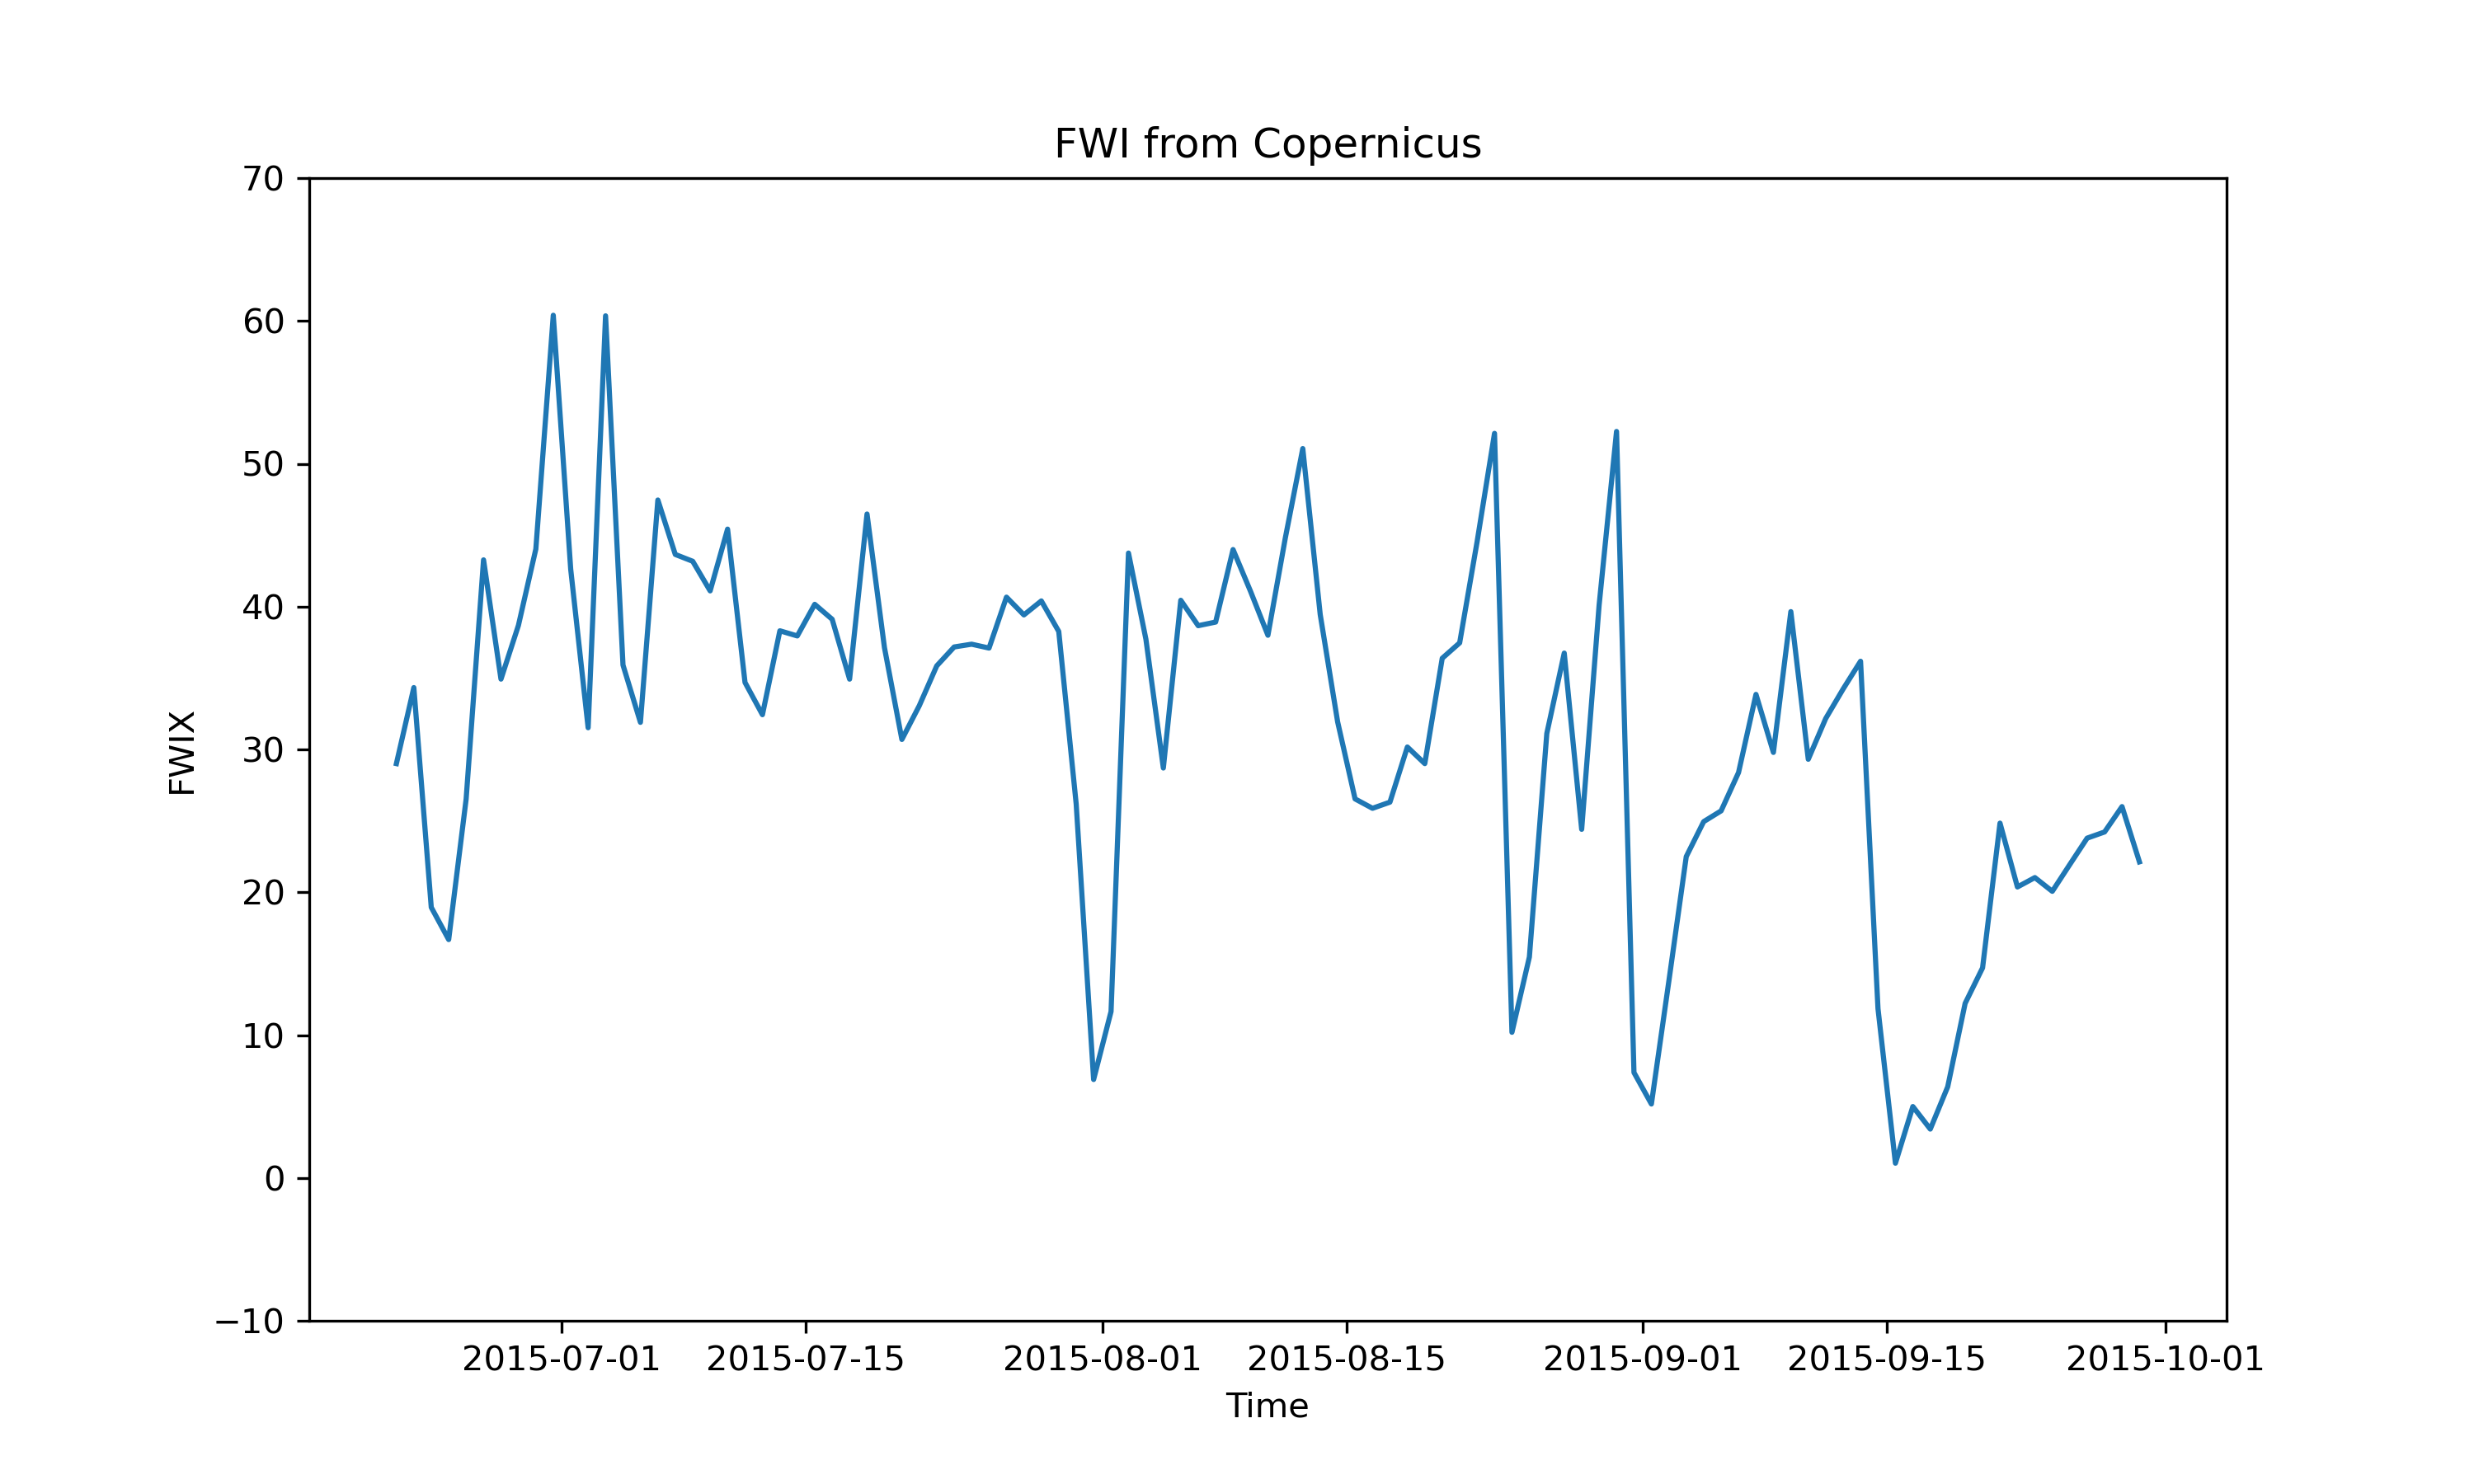
\includegraphics[width=\textwidth]{graphs/2015MesmoSitio/2015CopernicusFWI12.png}
        \caption{FWI - Copernicus}
        \label{fig:fwi_copernicus_2015_semfogo}
    \end{subfigure}
    \hfill
    \begin{subfigure}{0.49\textwidth}
        \centering
        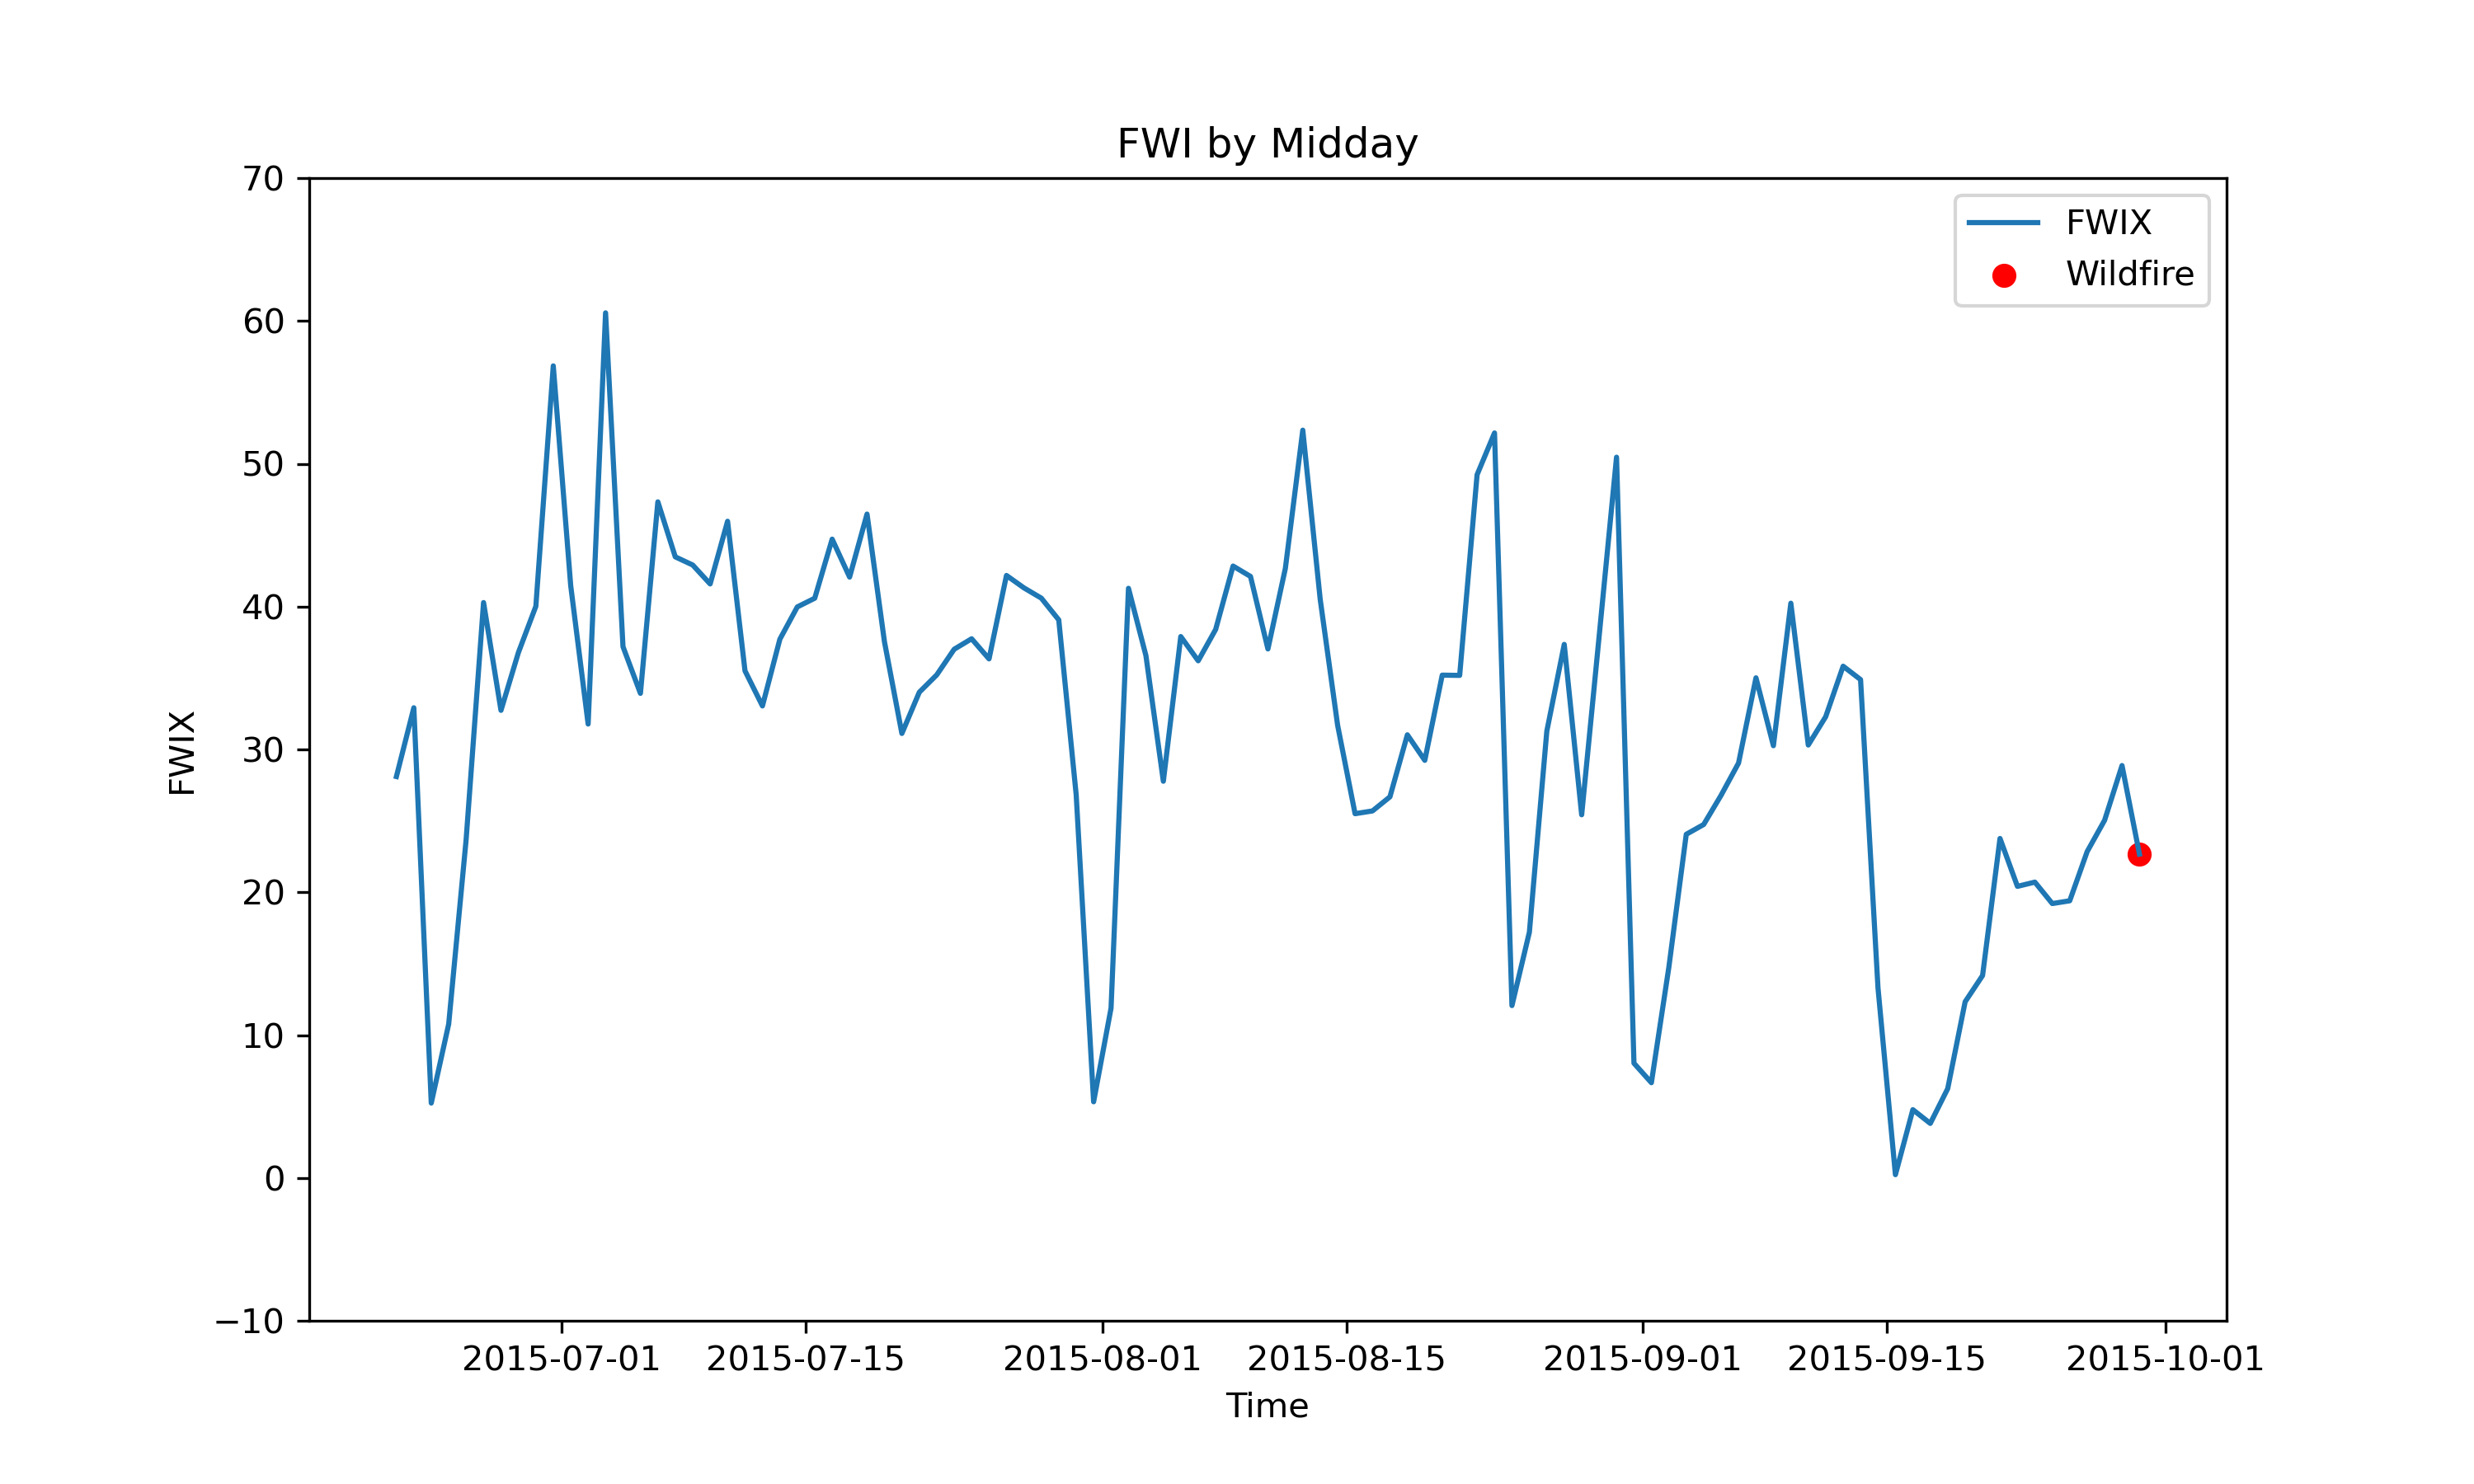
\includegraphics[width=\textwidth]{graphs/2015MesmoSitio/2015CalcFWI12.png}
        \caption{FWI - Calculated value}
        \label{fig:fwi_calculated_2015_semfogo}
    \end{subfigure}
    \label{fig:comparison_semfogo_copernicus_calculated}
\end{figure}

\begin{figure}[h]
\caption{Comparison of FFMC calculated values and Copernicus}
    \centering
    \begin{subfigure}{0.49\textwidth}
        \centering
        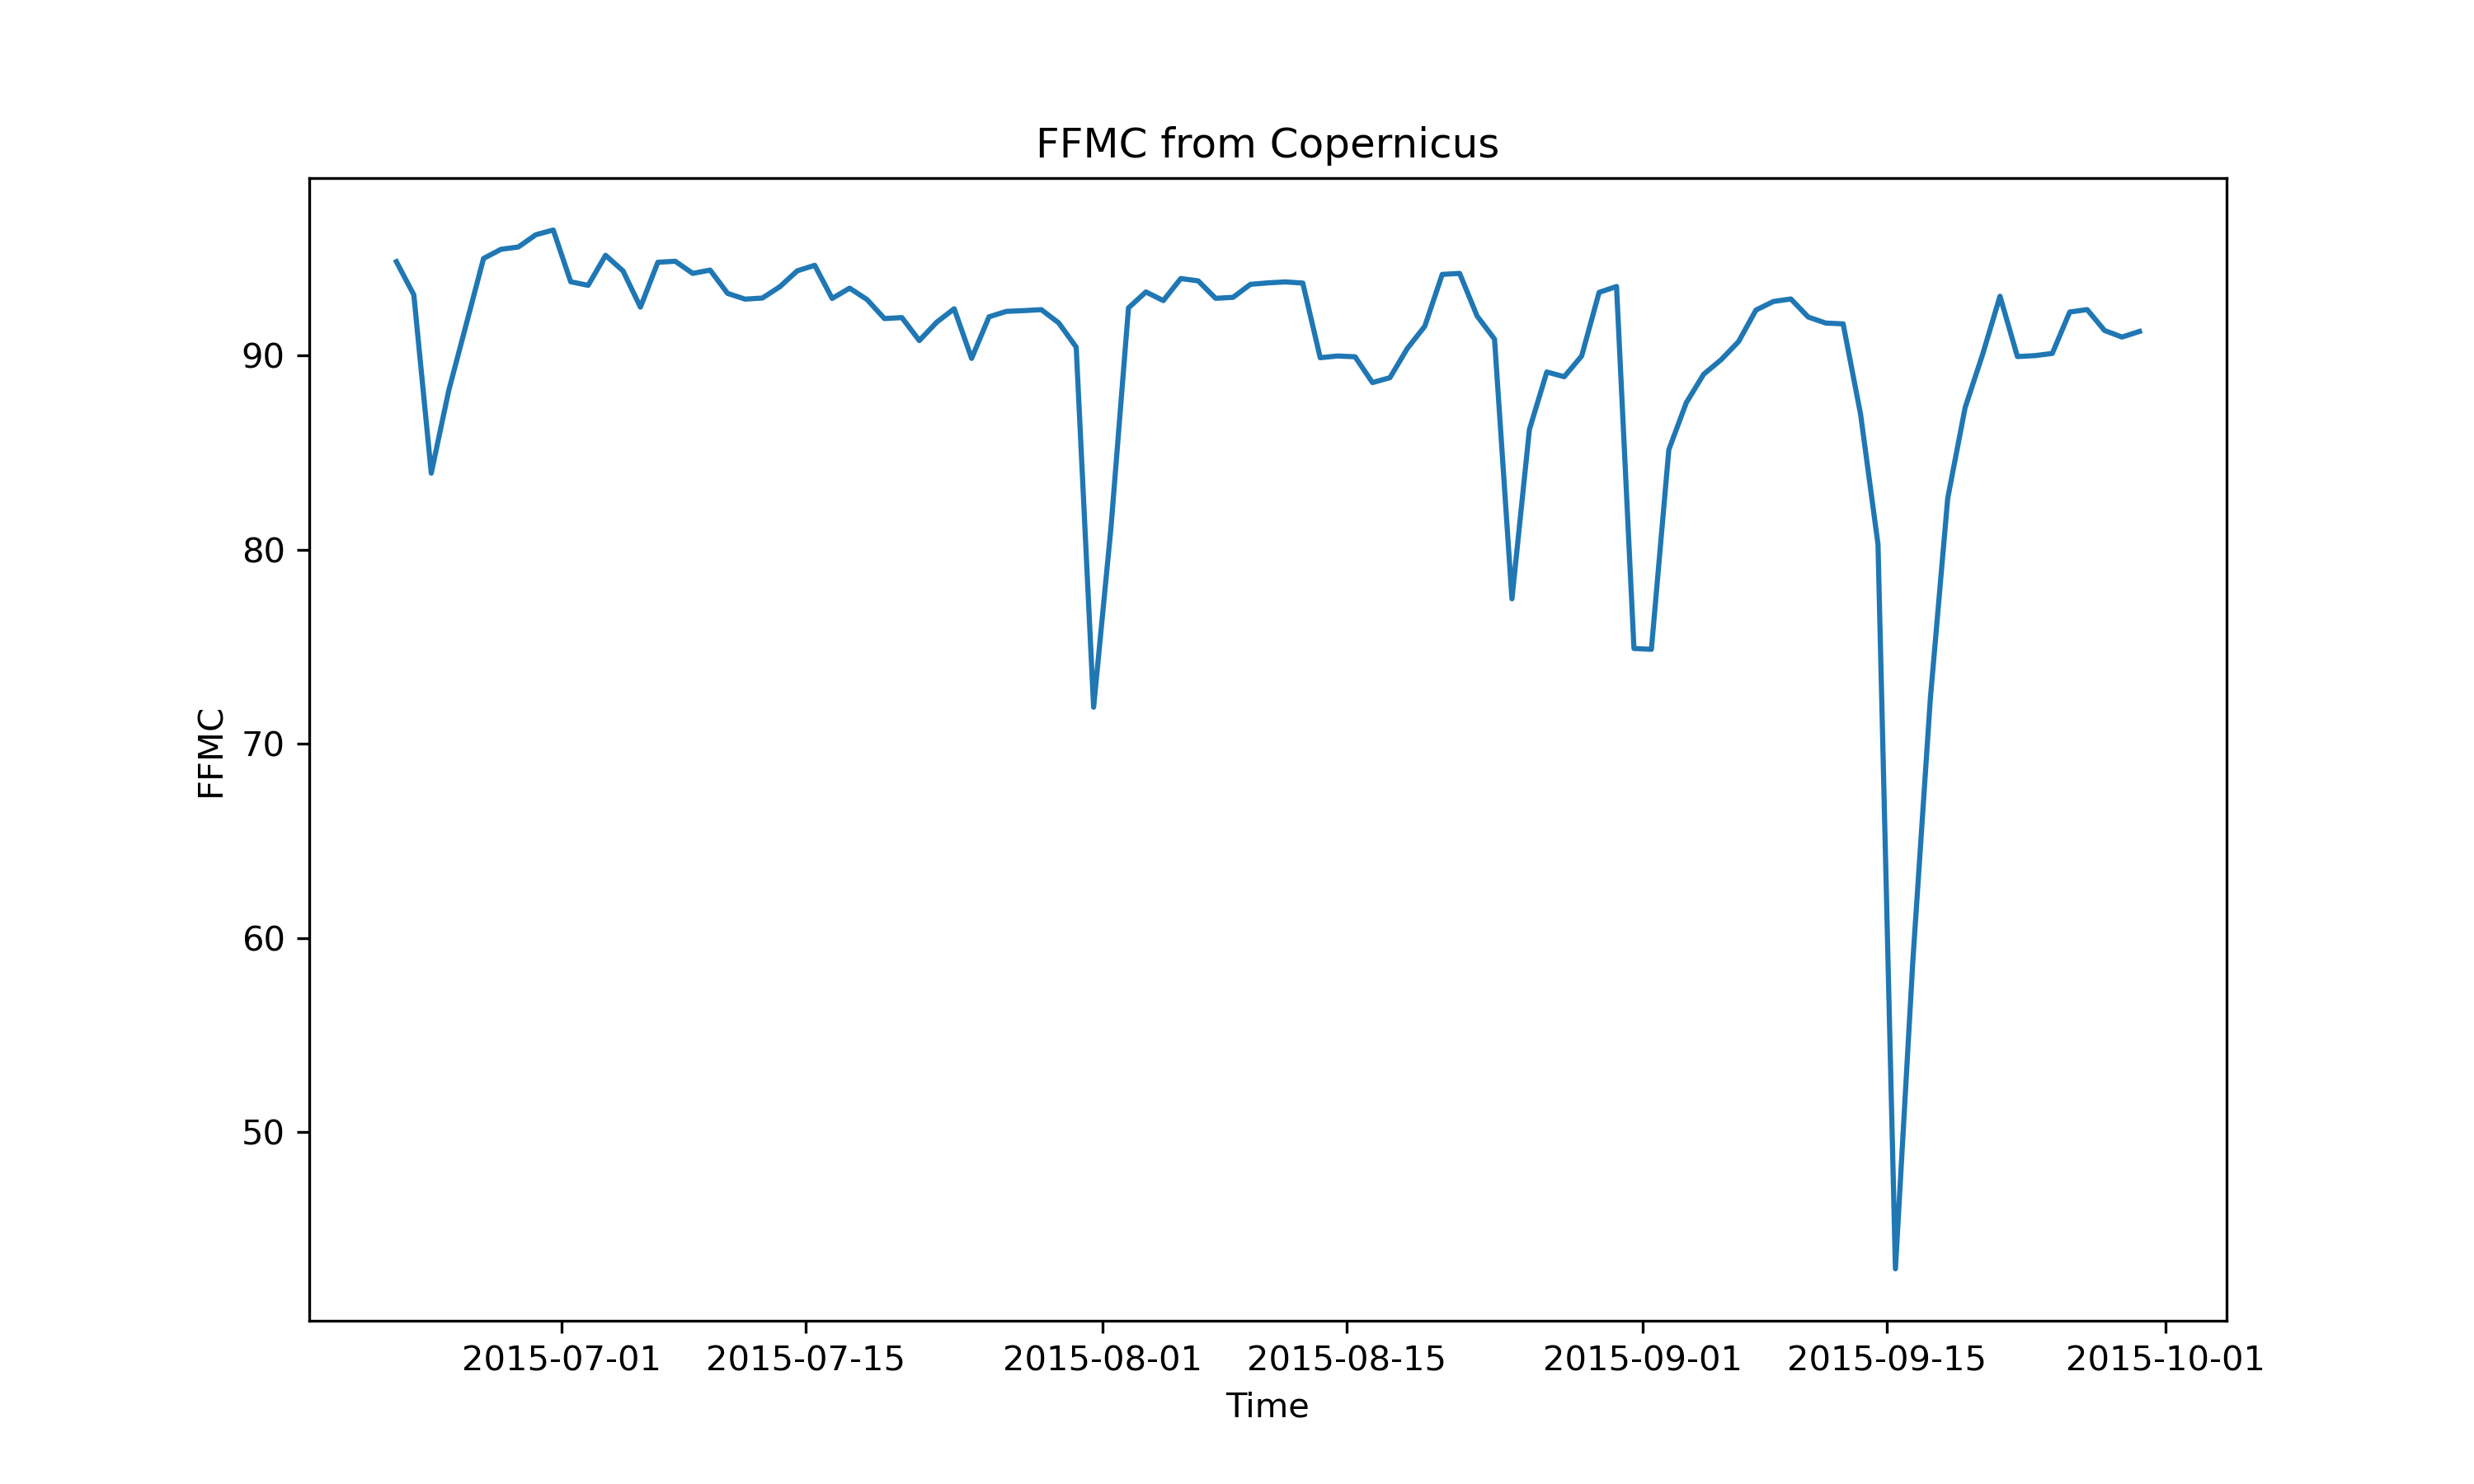
\includegraphics[width=\textwidth]{graphs/2015MesmoSitio/2015CopernicusFFMC12.png}
        \caption{FFMC - Copernicus}
        \label{fig:ffmc_copernicus_2015_semfogo}
    \end{subfigure}
    \hfill
    \begin{subfigure}{0.49\textwidth}
        \centering
        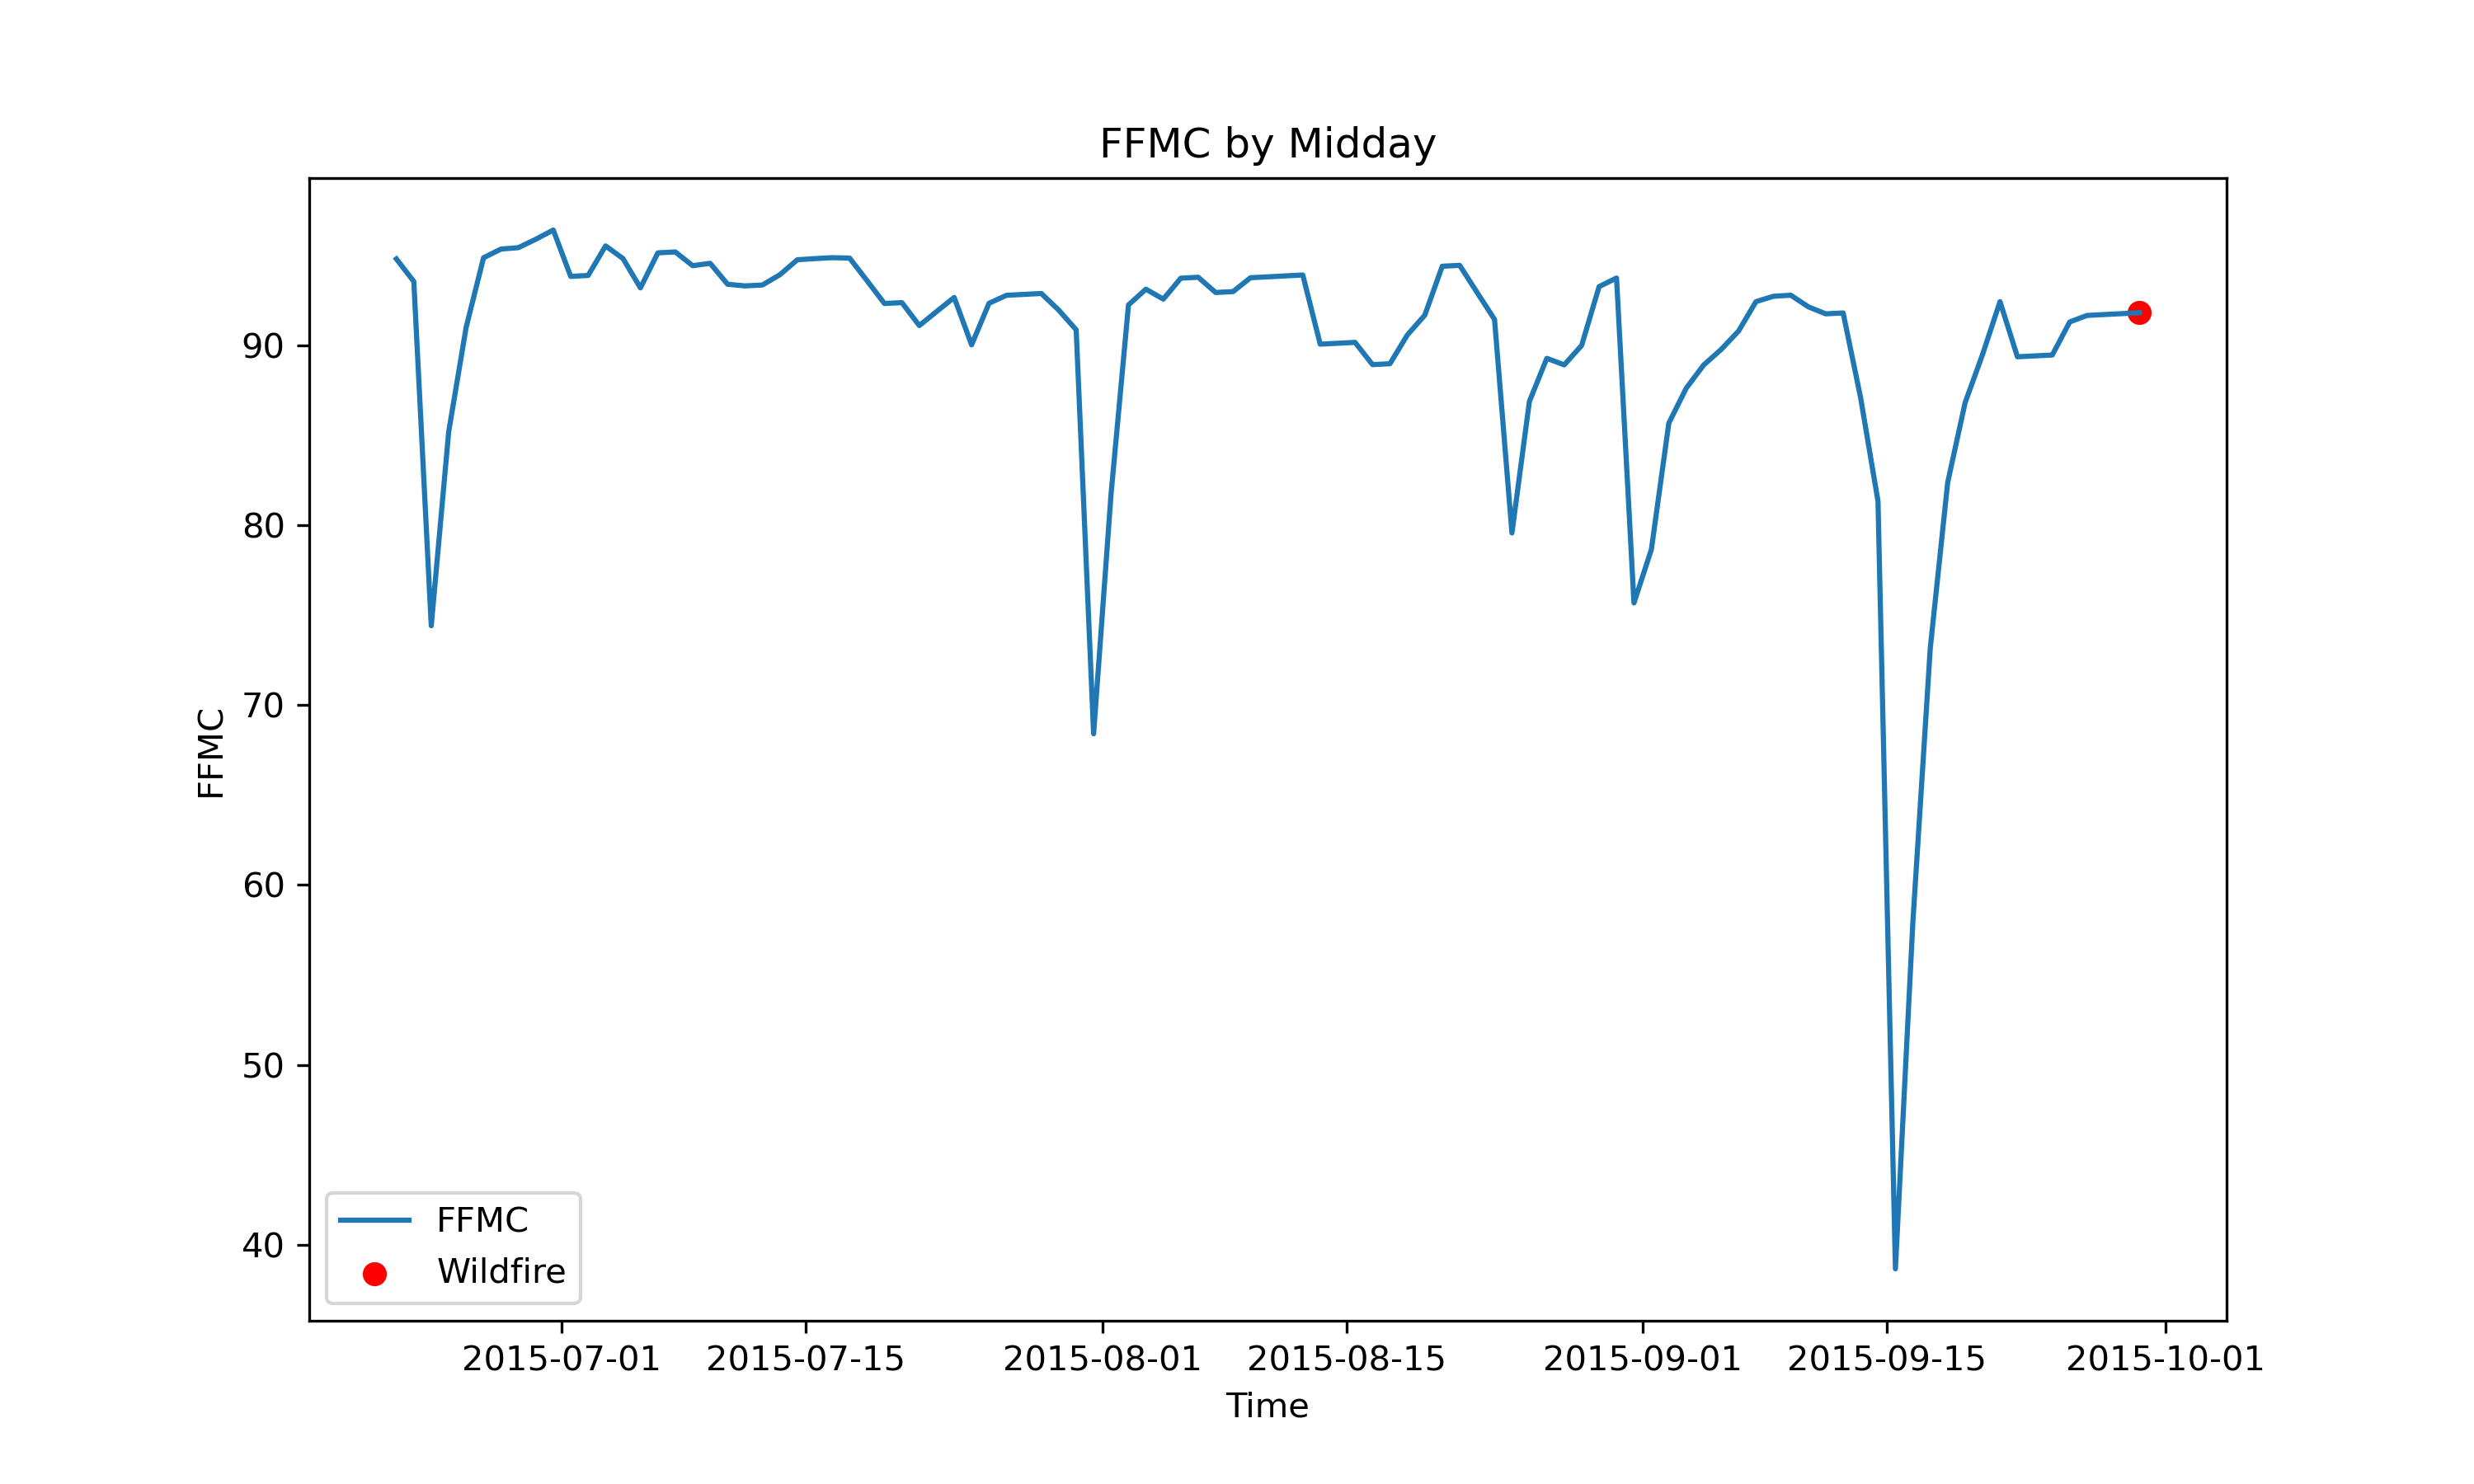
\includegraphics[width=\textwidth]{graphs/2015MesmoSitio/2015CalcFFMC12.png}
        \caption{FFMC - Calculated value}
        \label{fig:ffmc_calculated_2015_semfogo}
    \end{subfigure}
    \label{fig:comparison_ffmc_semfogo_copernicus_calculated}
\end{figure}

\begin{figure}[h]
\caption{Comparison of DMC calculated values and Copernicus}
    \centering
    \begin{subfigure}{0.49\textwidth}
        \centering
        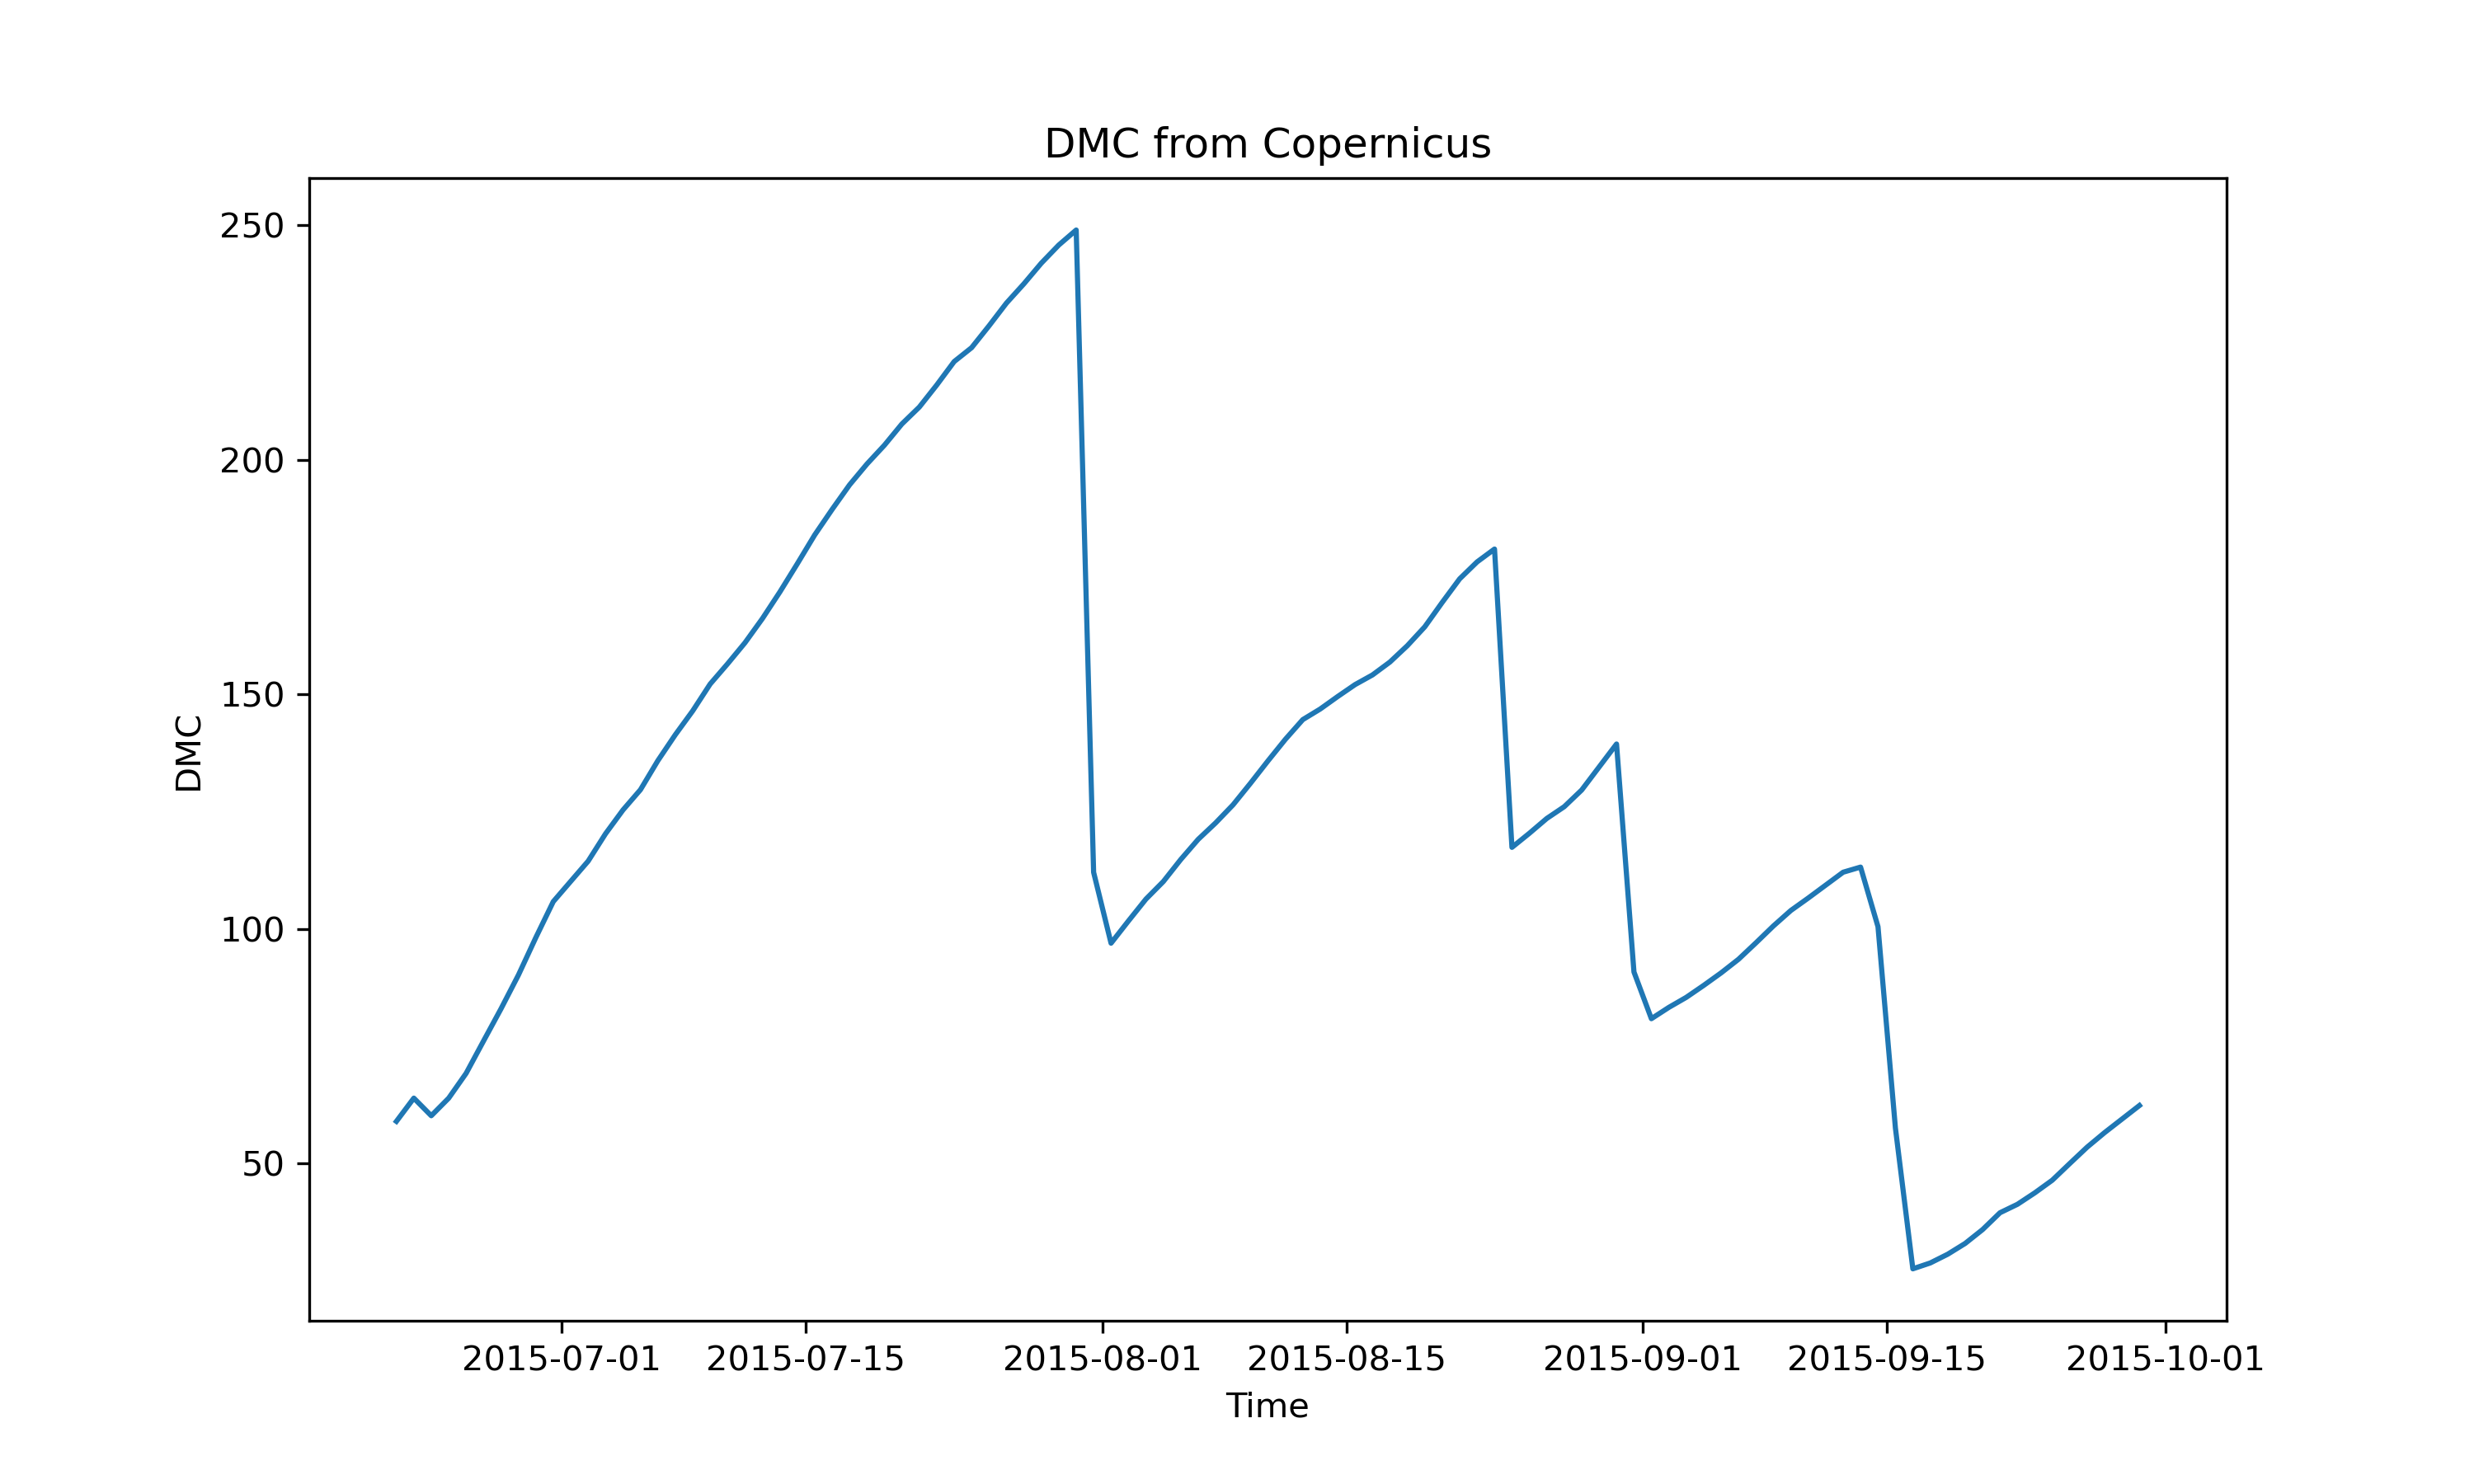
\includegraphics[width=\textwidth]{graphs/2015MesmoSitio/2015CopernicusDMC12.png}
        \caption{DMC - Copernicus}
        \label{fig:dmc_copernicus_2015_semfogo}
    \end{subfigure}
    \hfill
    \begin{subfigure}{0.49\textwidth}
        \centering
        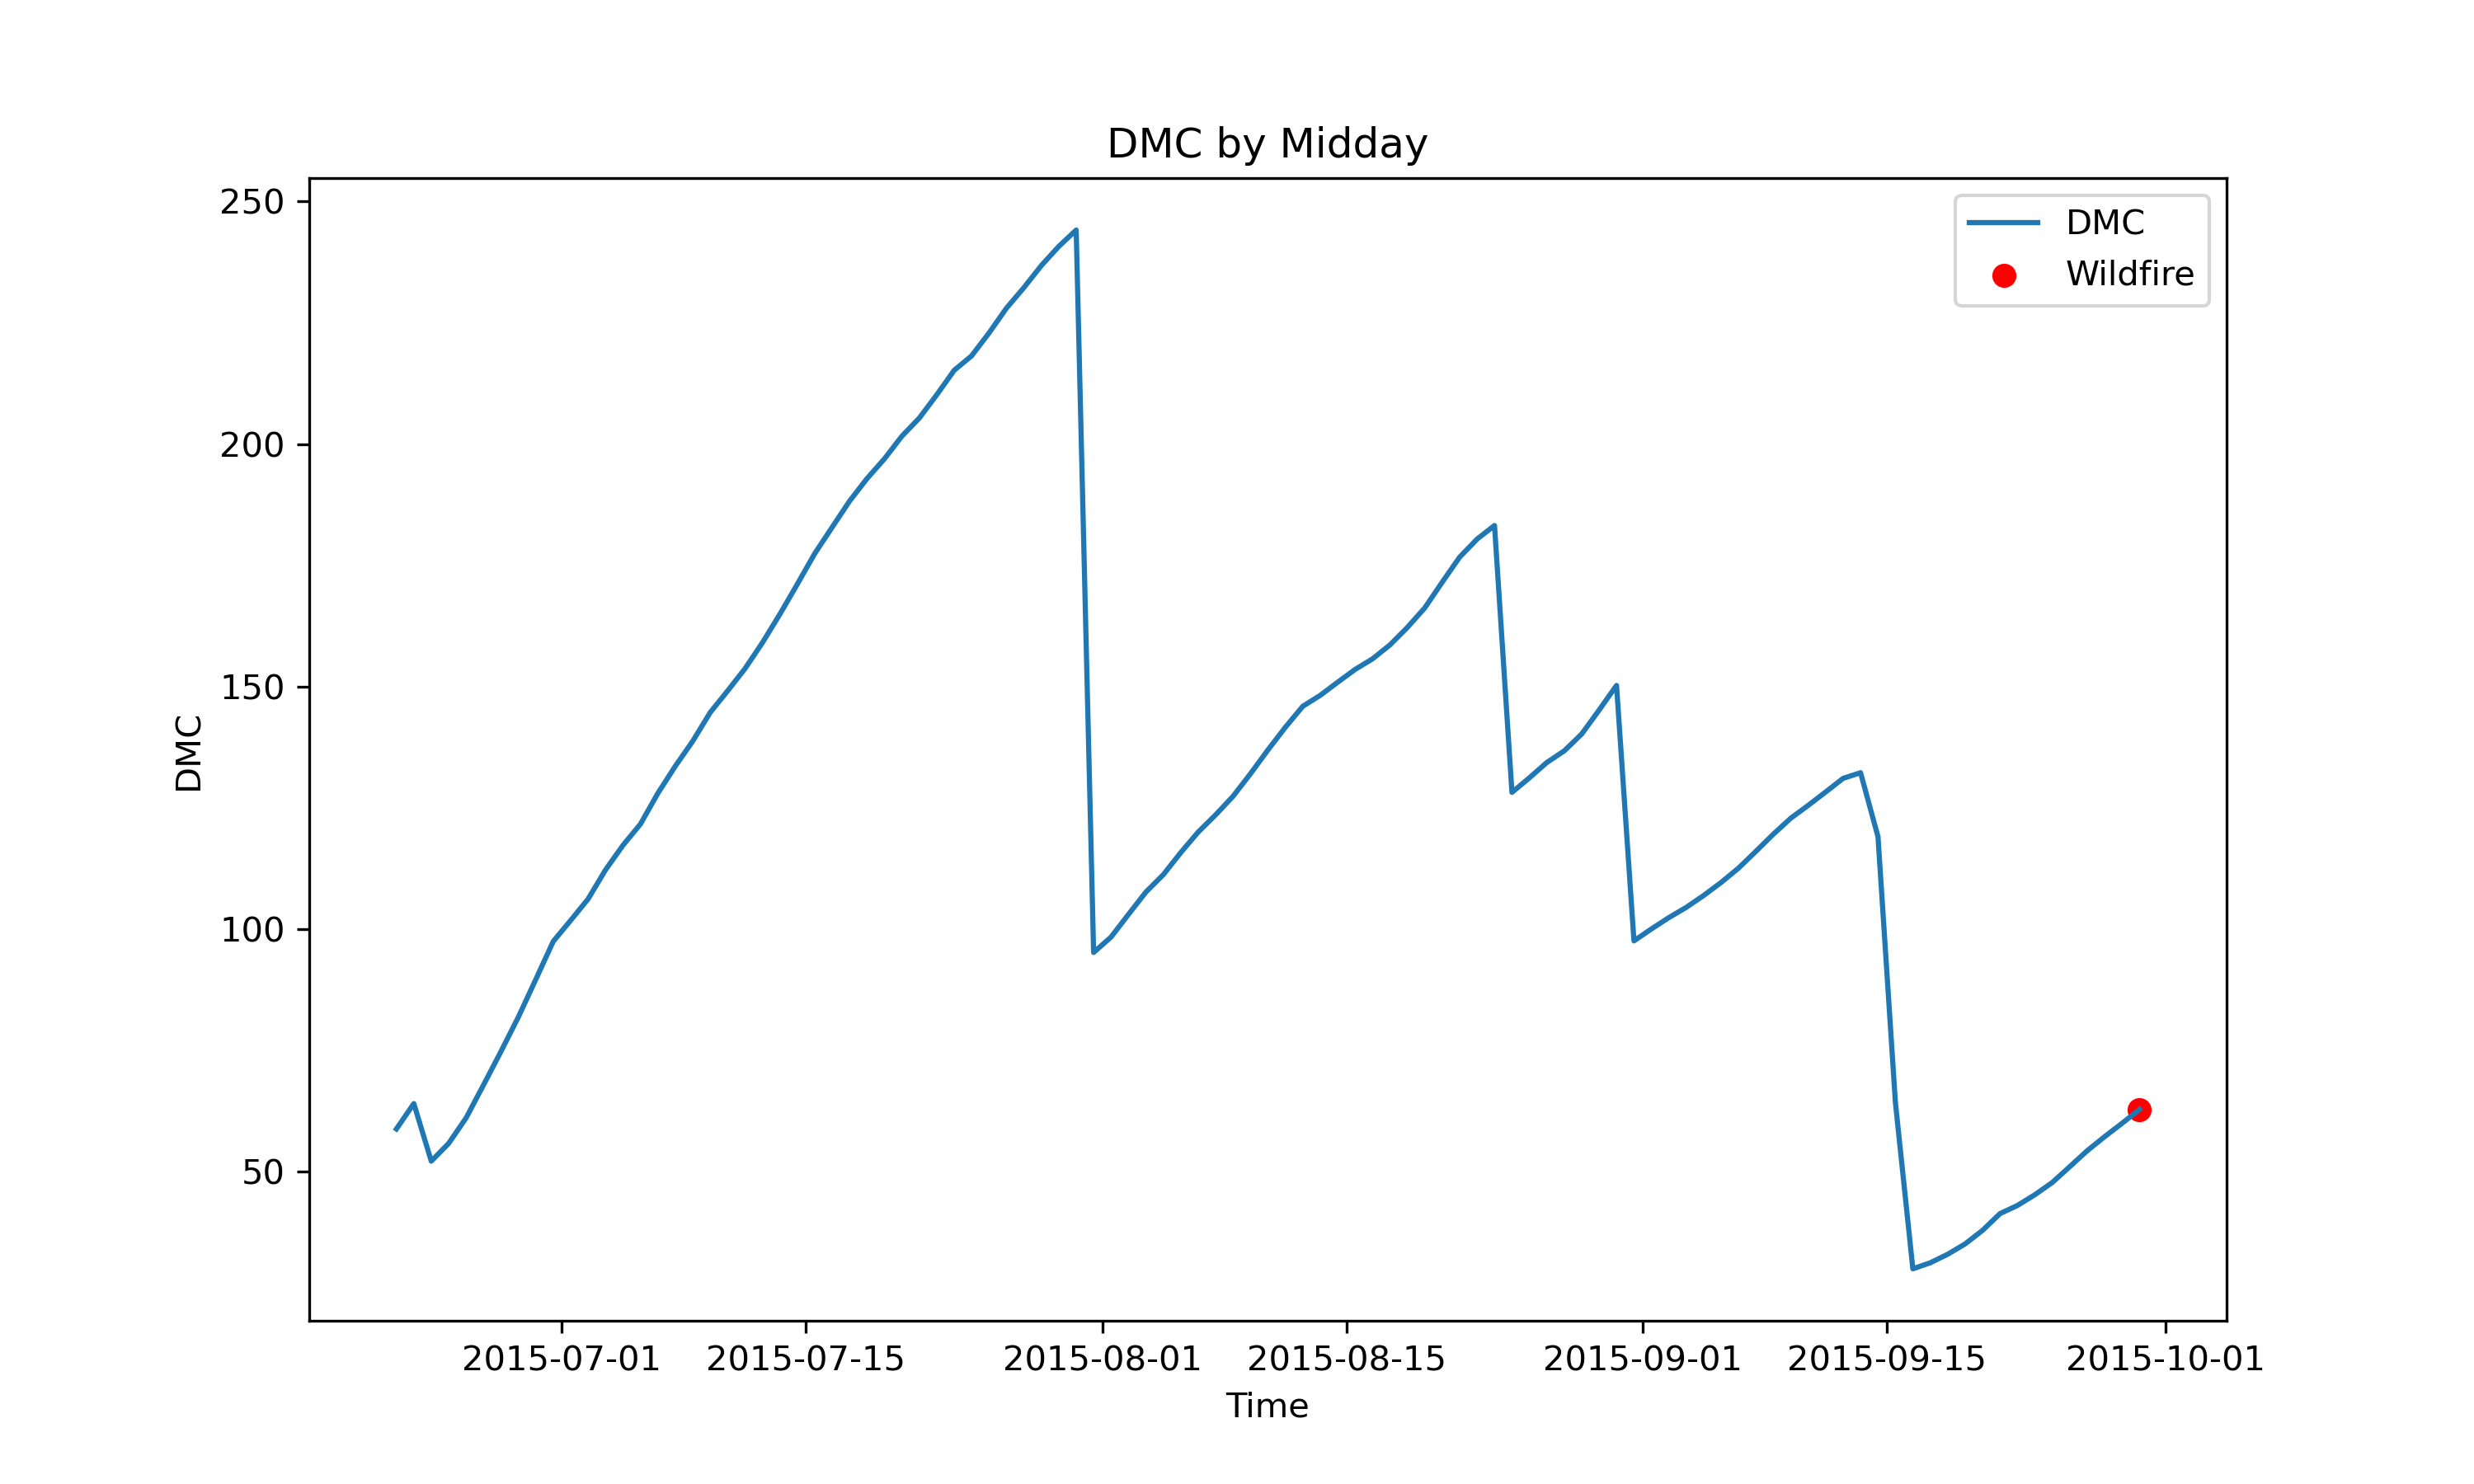
\includegraphics[width=\textwidth]{graphs/2015MesmoSitio/2015CalcDMC12.png}
        \caption{DMC - Calculated value}
        \label{fig:dmc_calculated_2015_semfogo}
    \end{subfigure}
    \label{fig:comparison_dmc_semfogo_copernicus_calculated}
\end{figure}

\begin{figure}[h]
\caption{Comparison of DC calculated values and Copernicus}
    \centering
    \begin{subfigure}{0.49\textwidth}
        \centering
        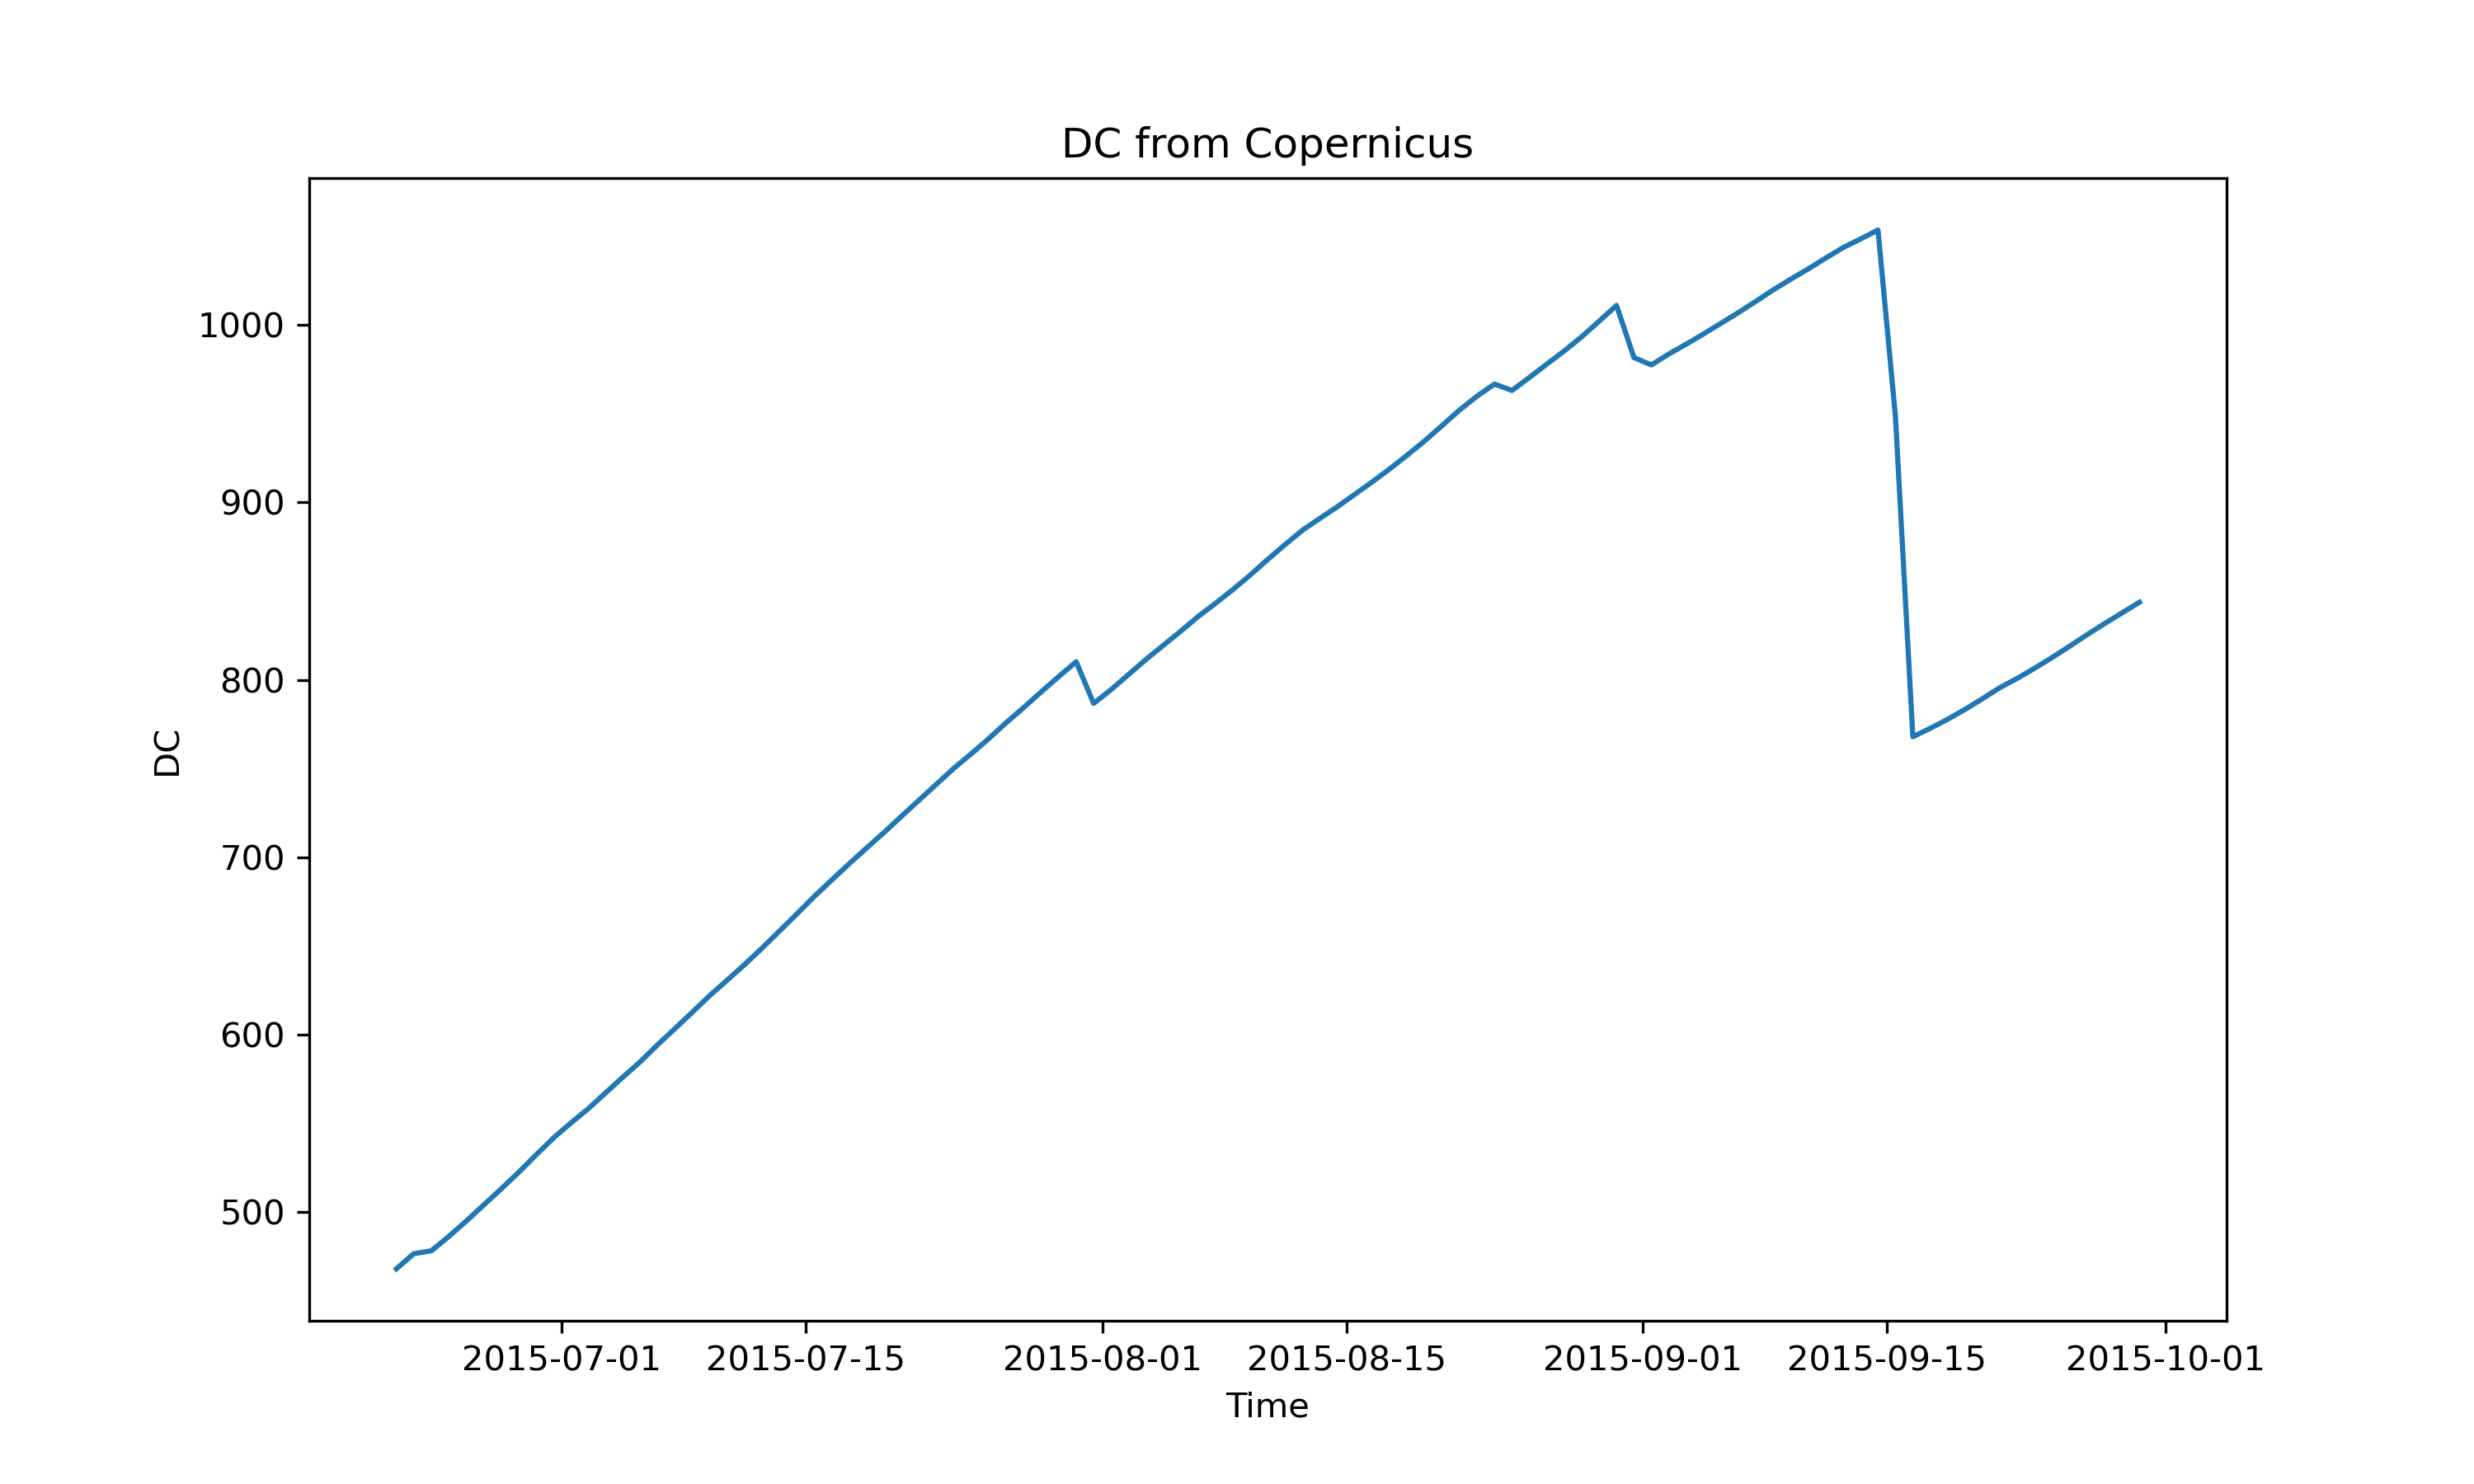
\includegraphics[width=\textwidth]{graphs/2015MesmoSitio/2015CopernicusDC12.png}
        \caption{DC - Copernicus}
        \label{fig:dc_copernicus_2015_semfogo}
    \end{subfigure}
    \hfill
    \begin{subfigure}{0.49\textwidth}
        \centering
        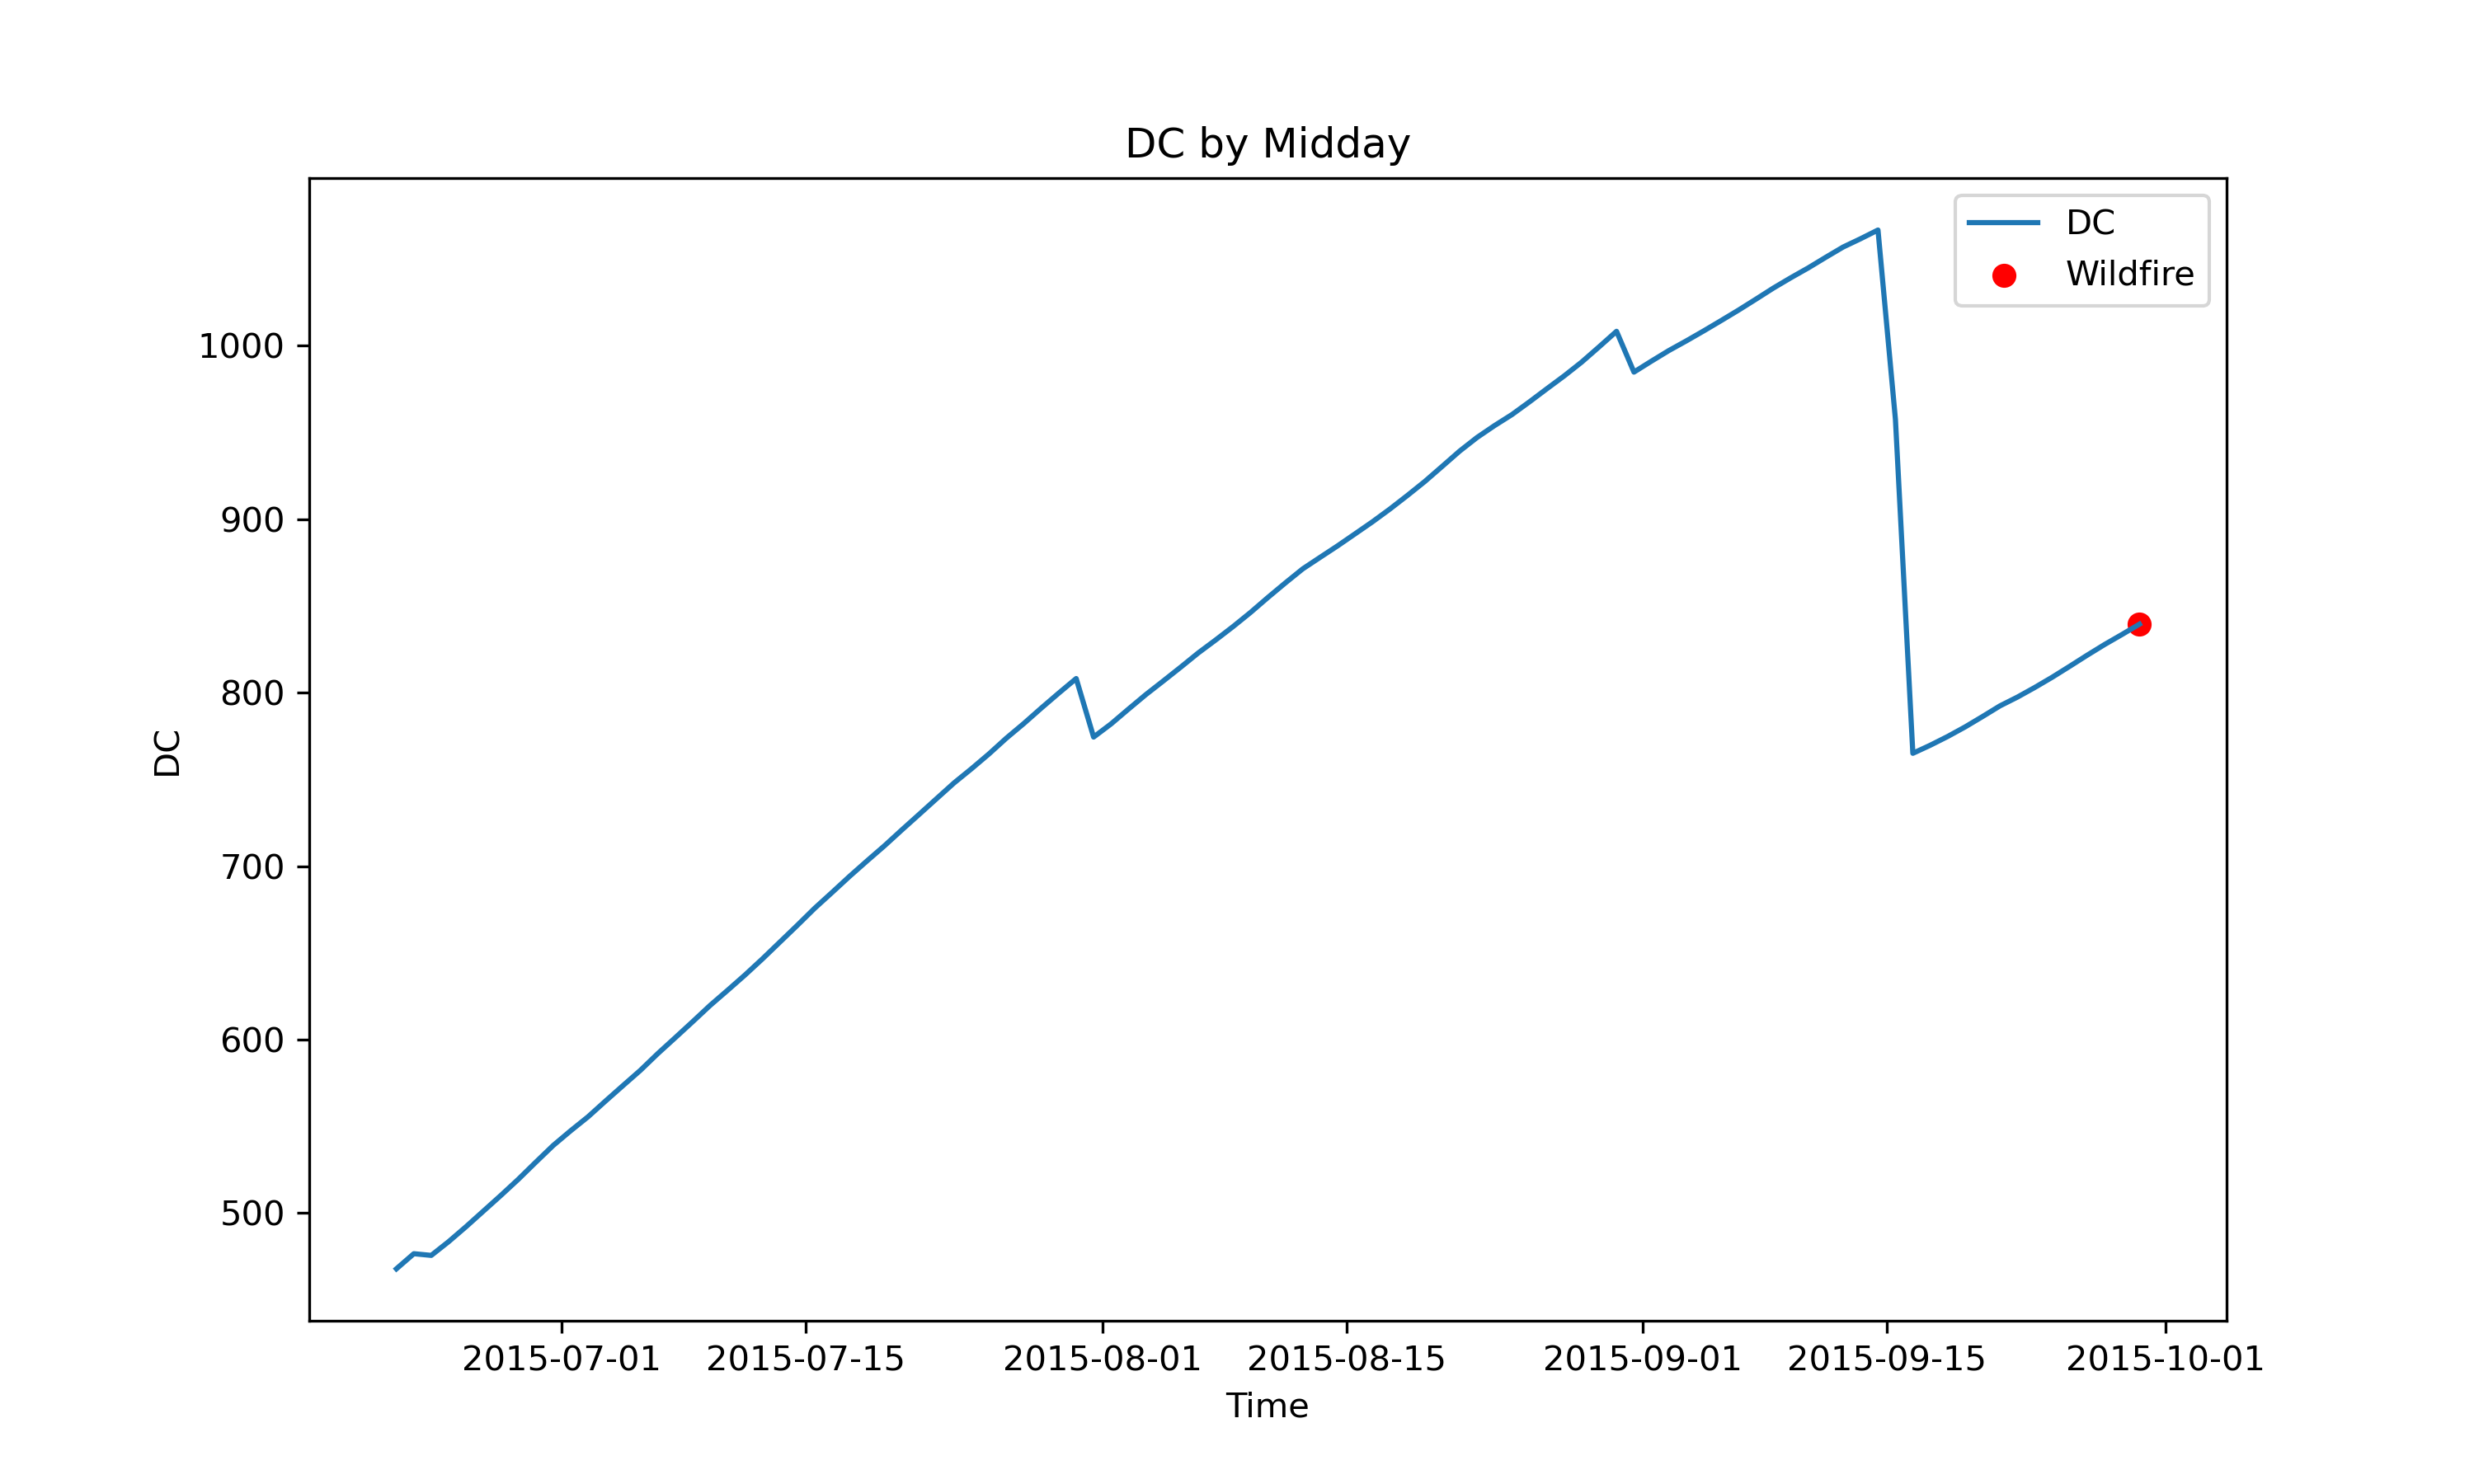
\includegraphics[width=\textwidth]{graphs/2015MesmoSitio/2015CalcDC12.png}
        \caption{DC - Calculated value}
        \label{fig:dc_calculated_2015_semfogo}
    \end{subfigure}
    \label{fig:comparison_dc_semfogo_copernicus_calculated}
\end{figure}

\begin{figure}[h]
\caption{Comparison of ISI calculated values and Copernicus}
    \centering
    \begin{subfigure}{0.49\textwidth}
        \centering
        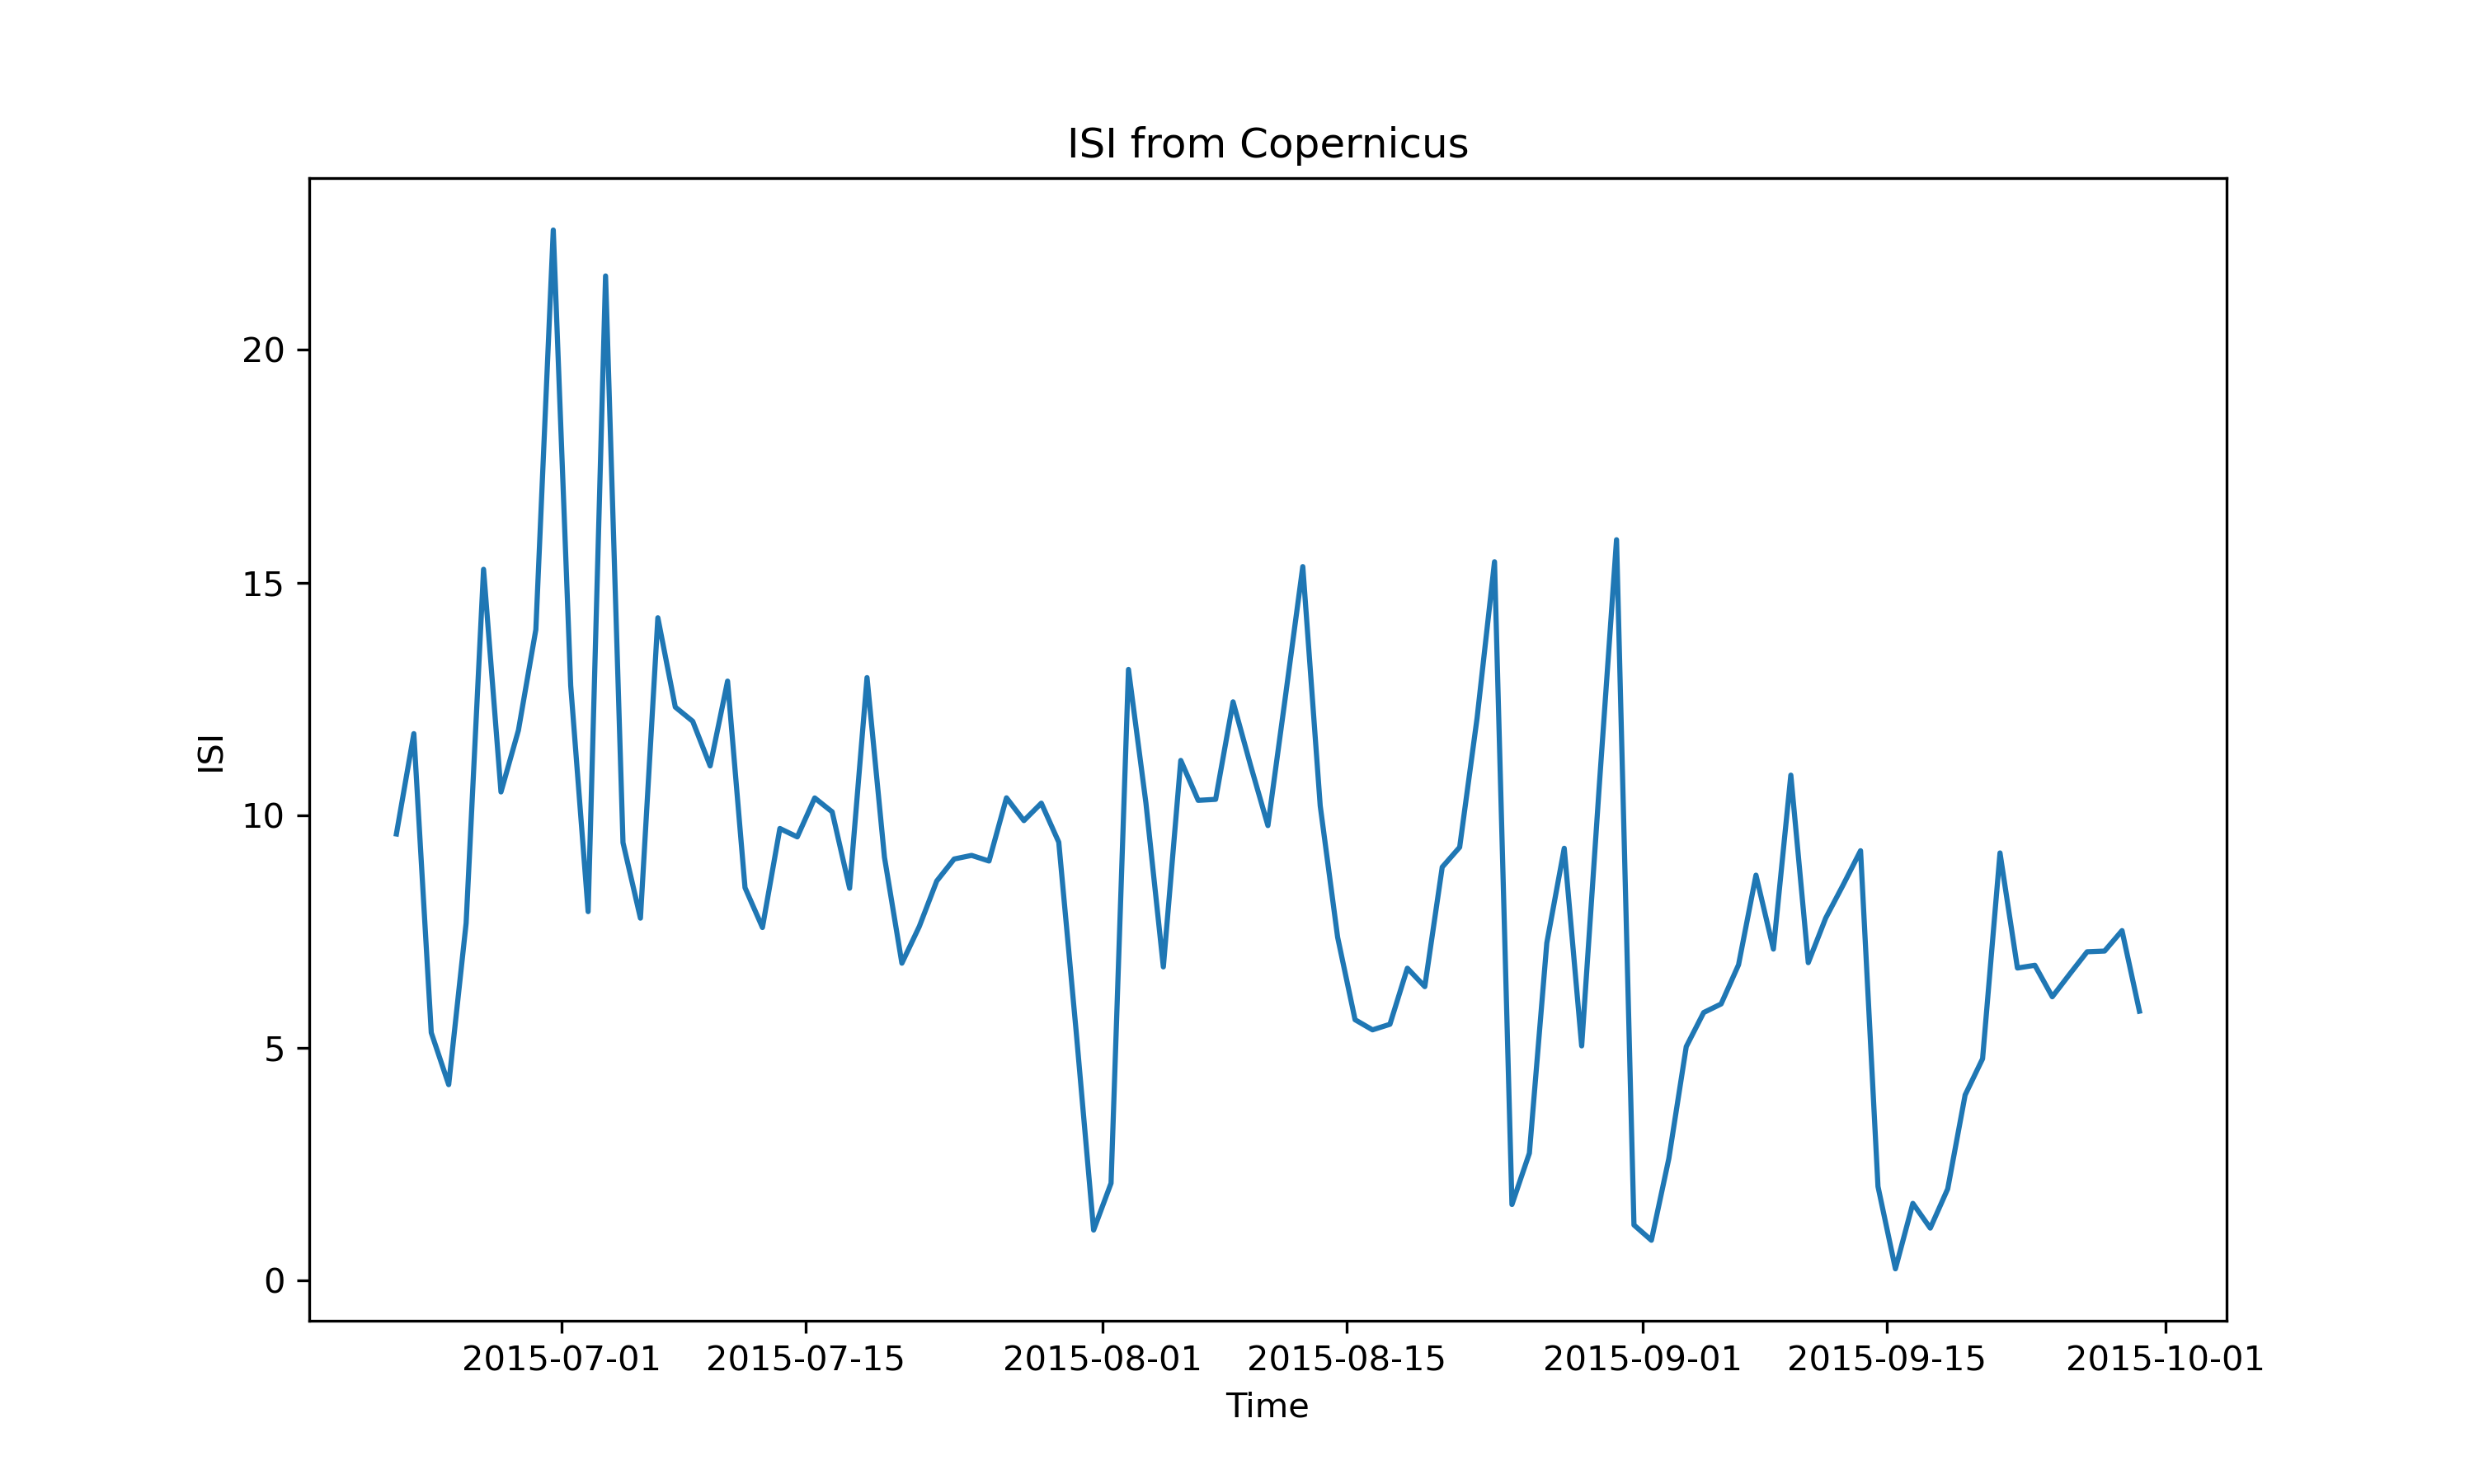
\includegraphics[width=\textwidth]{graphs/2015MesmoSitio/2015CopernicusISI12.png}
        \caption{ISI - Copernicus}
        \label{fig:isi_copernicus_2015_semfogo}
    \end{subfigure}
    \hfill
    \begin{subfigure}{0.49\textwidth}
        \centering
        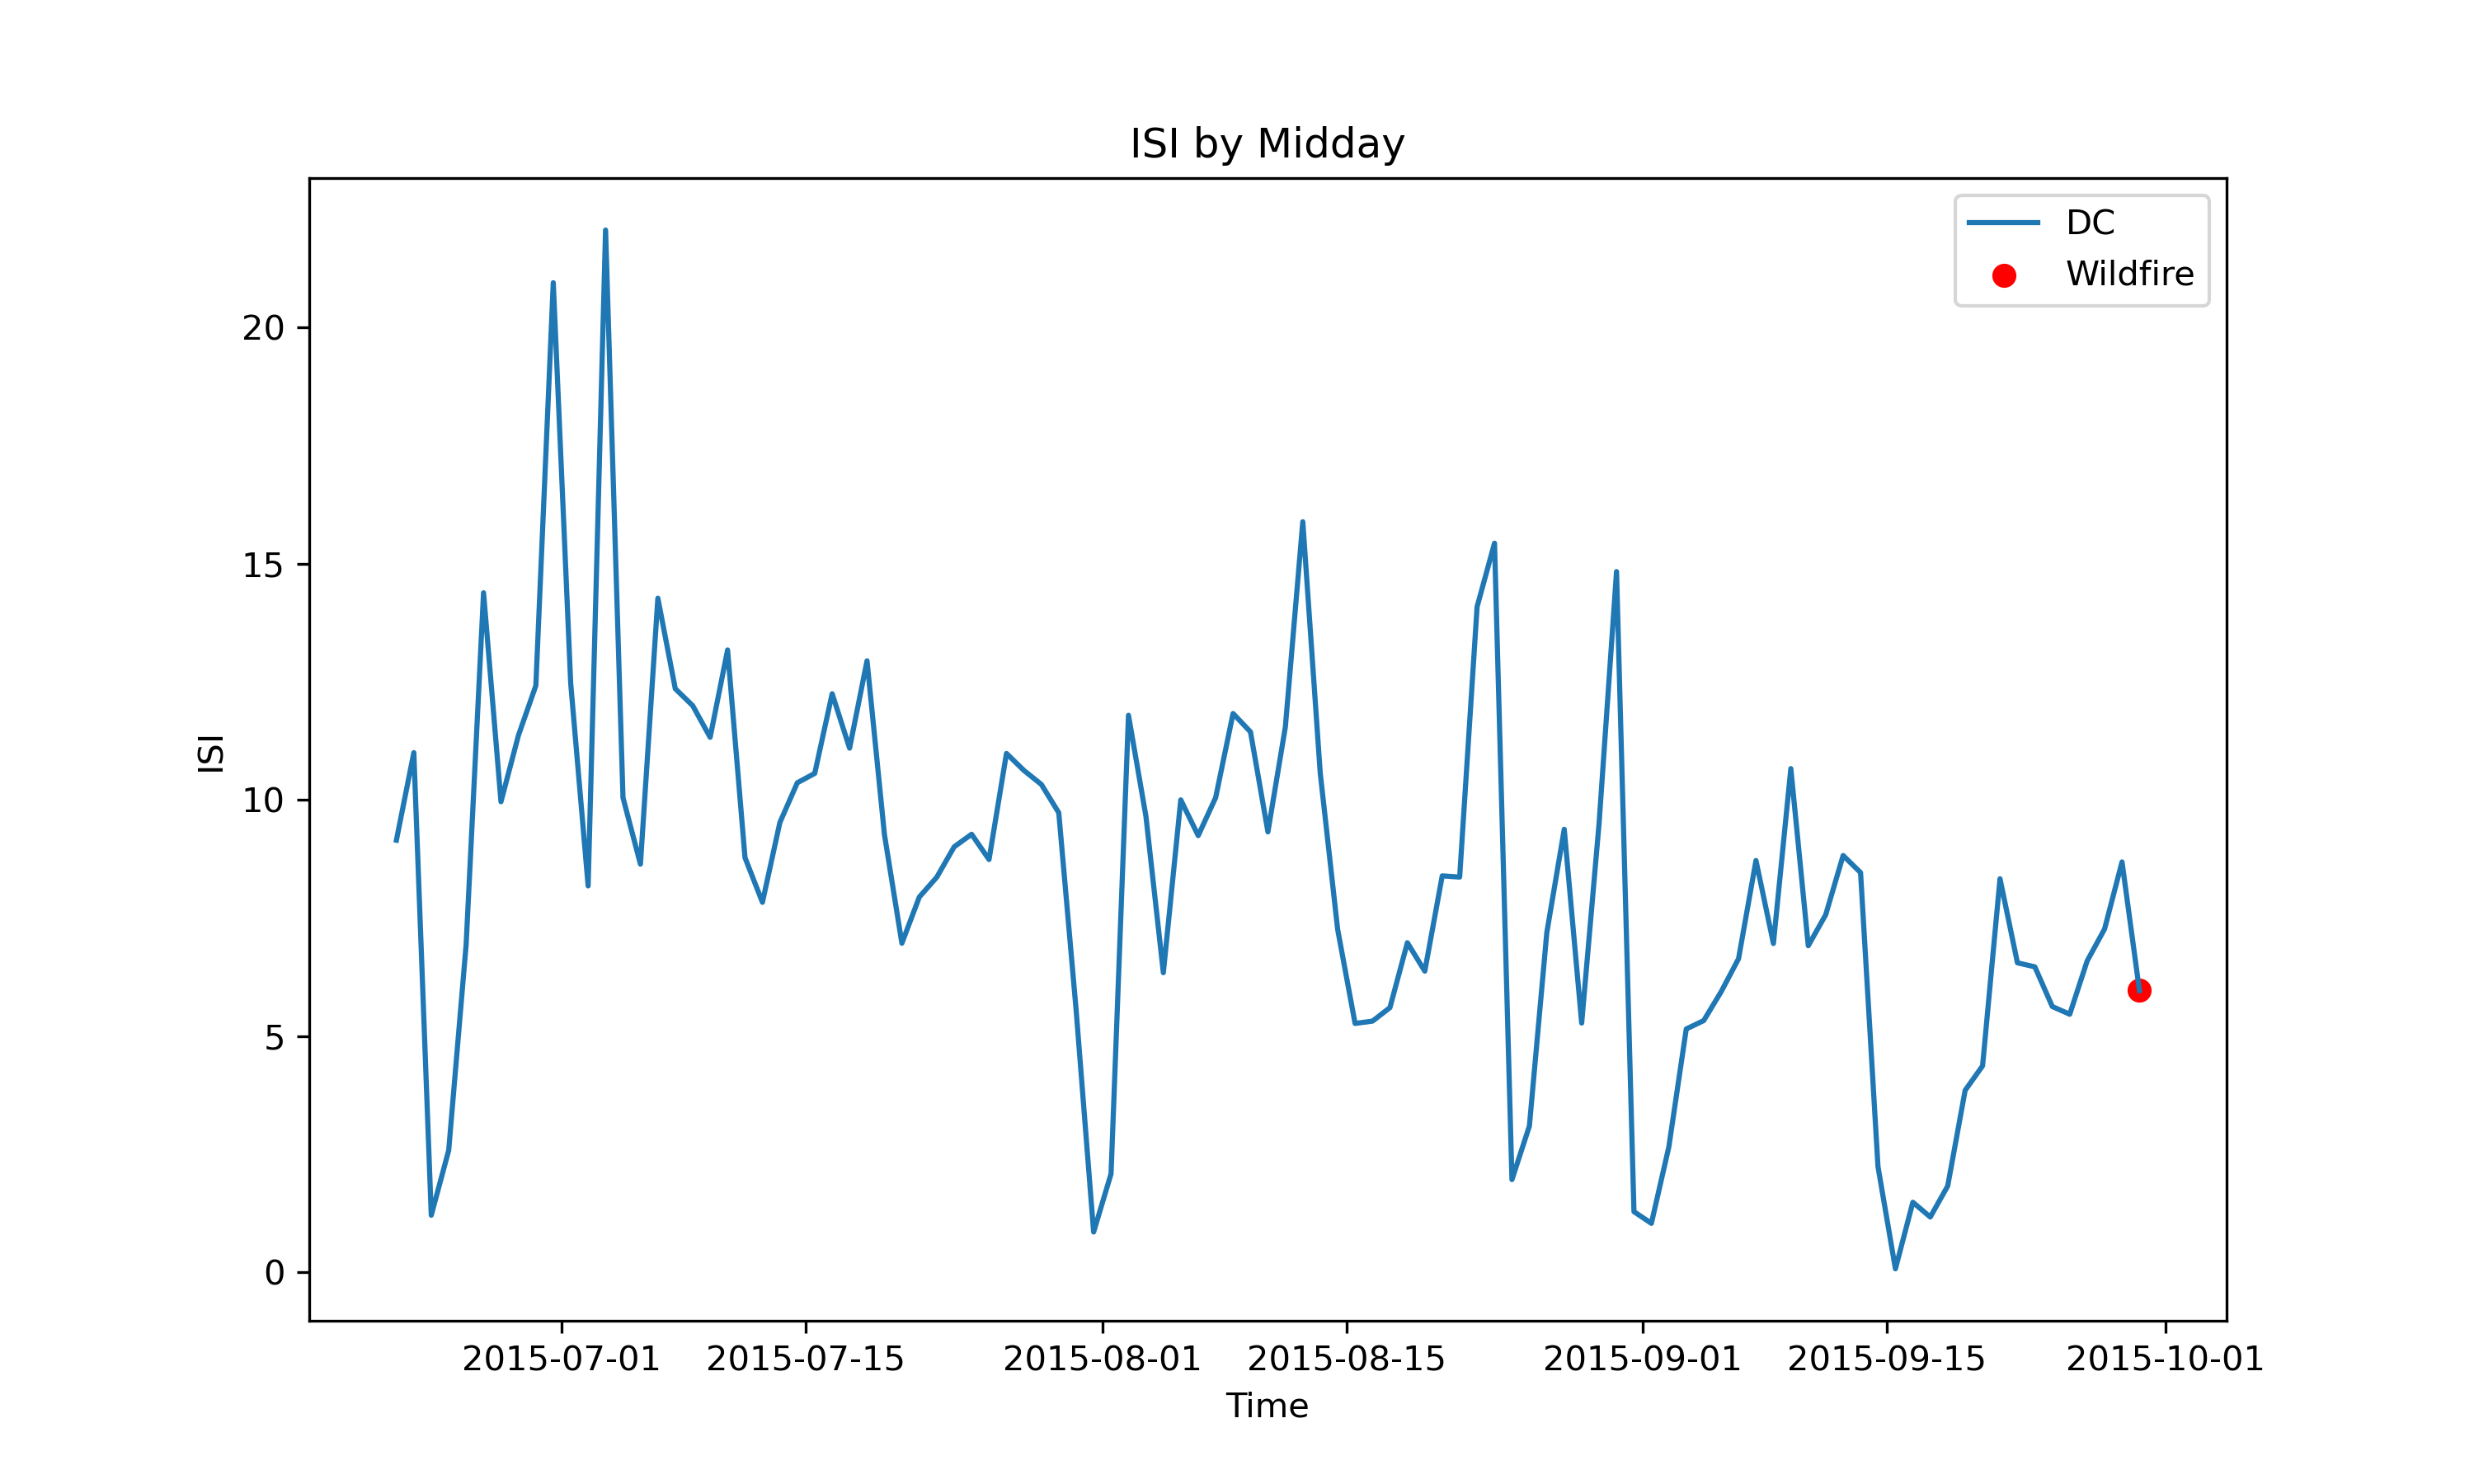
\includegraphics[width=\textwidth]{graphs/2015MesmoSitio/2015CalcISI12.png}
        \caption{ISI - Calculated value}
        \label{fig:isi_calculated_2015_semfogo}
    \end{subfigure}
    \label{fig:comparison_isi_semfogo_copernicus_calculated}
\end{figure}

\begin{figure}[h]
\caption{Comparison of BUI calculated values and Copernicus}
    \centering
    \begin{subfigure}{0.49\textwidth}
        \centering
        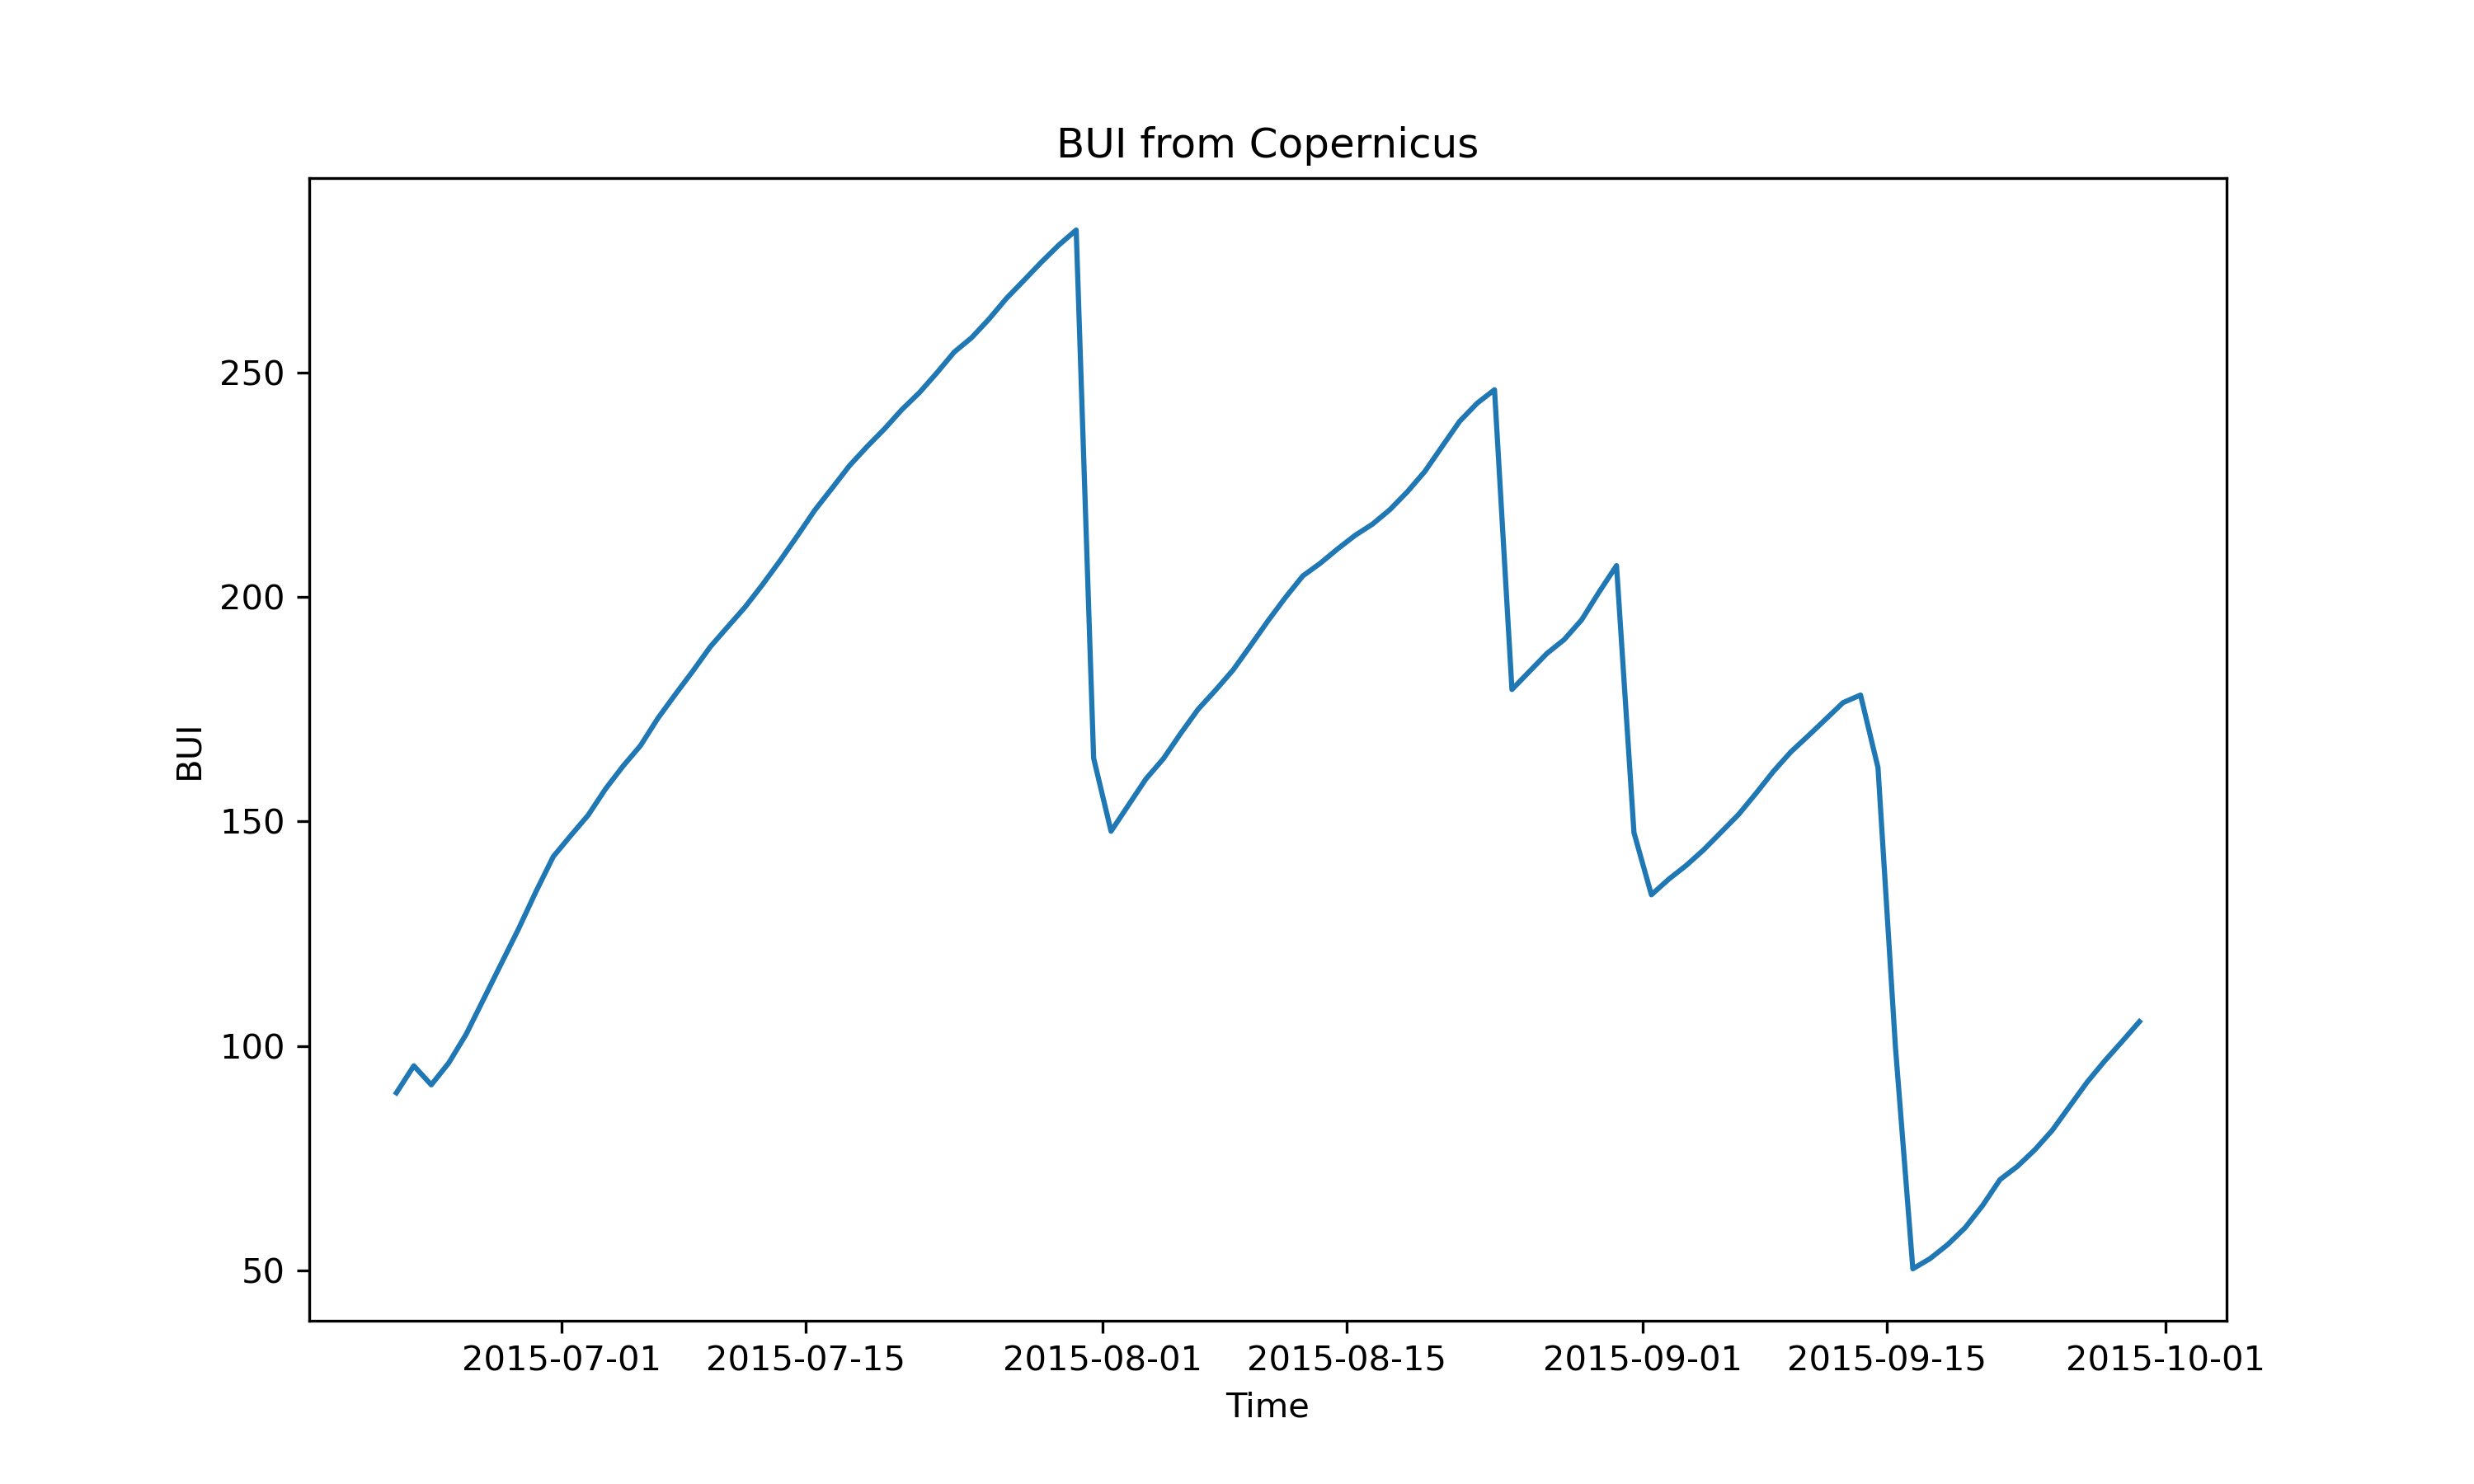
\includegraphics[width=\textwidth]{graphs/2015MesmoSitio/2015CopernicusBUI12.png}
        \caption{BUI - Copernicus}
        \label{fig:bui_copernicus_2015_semfogo}
    \end{subfigure}
    \hfill
    \begin{subfigure}{0.49\textwidth}
        \centering
        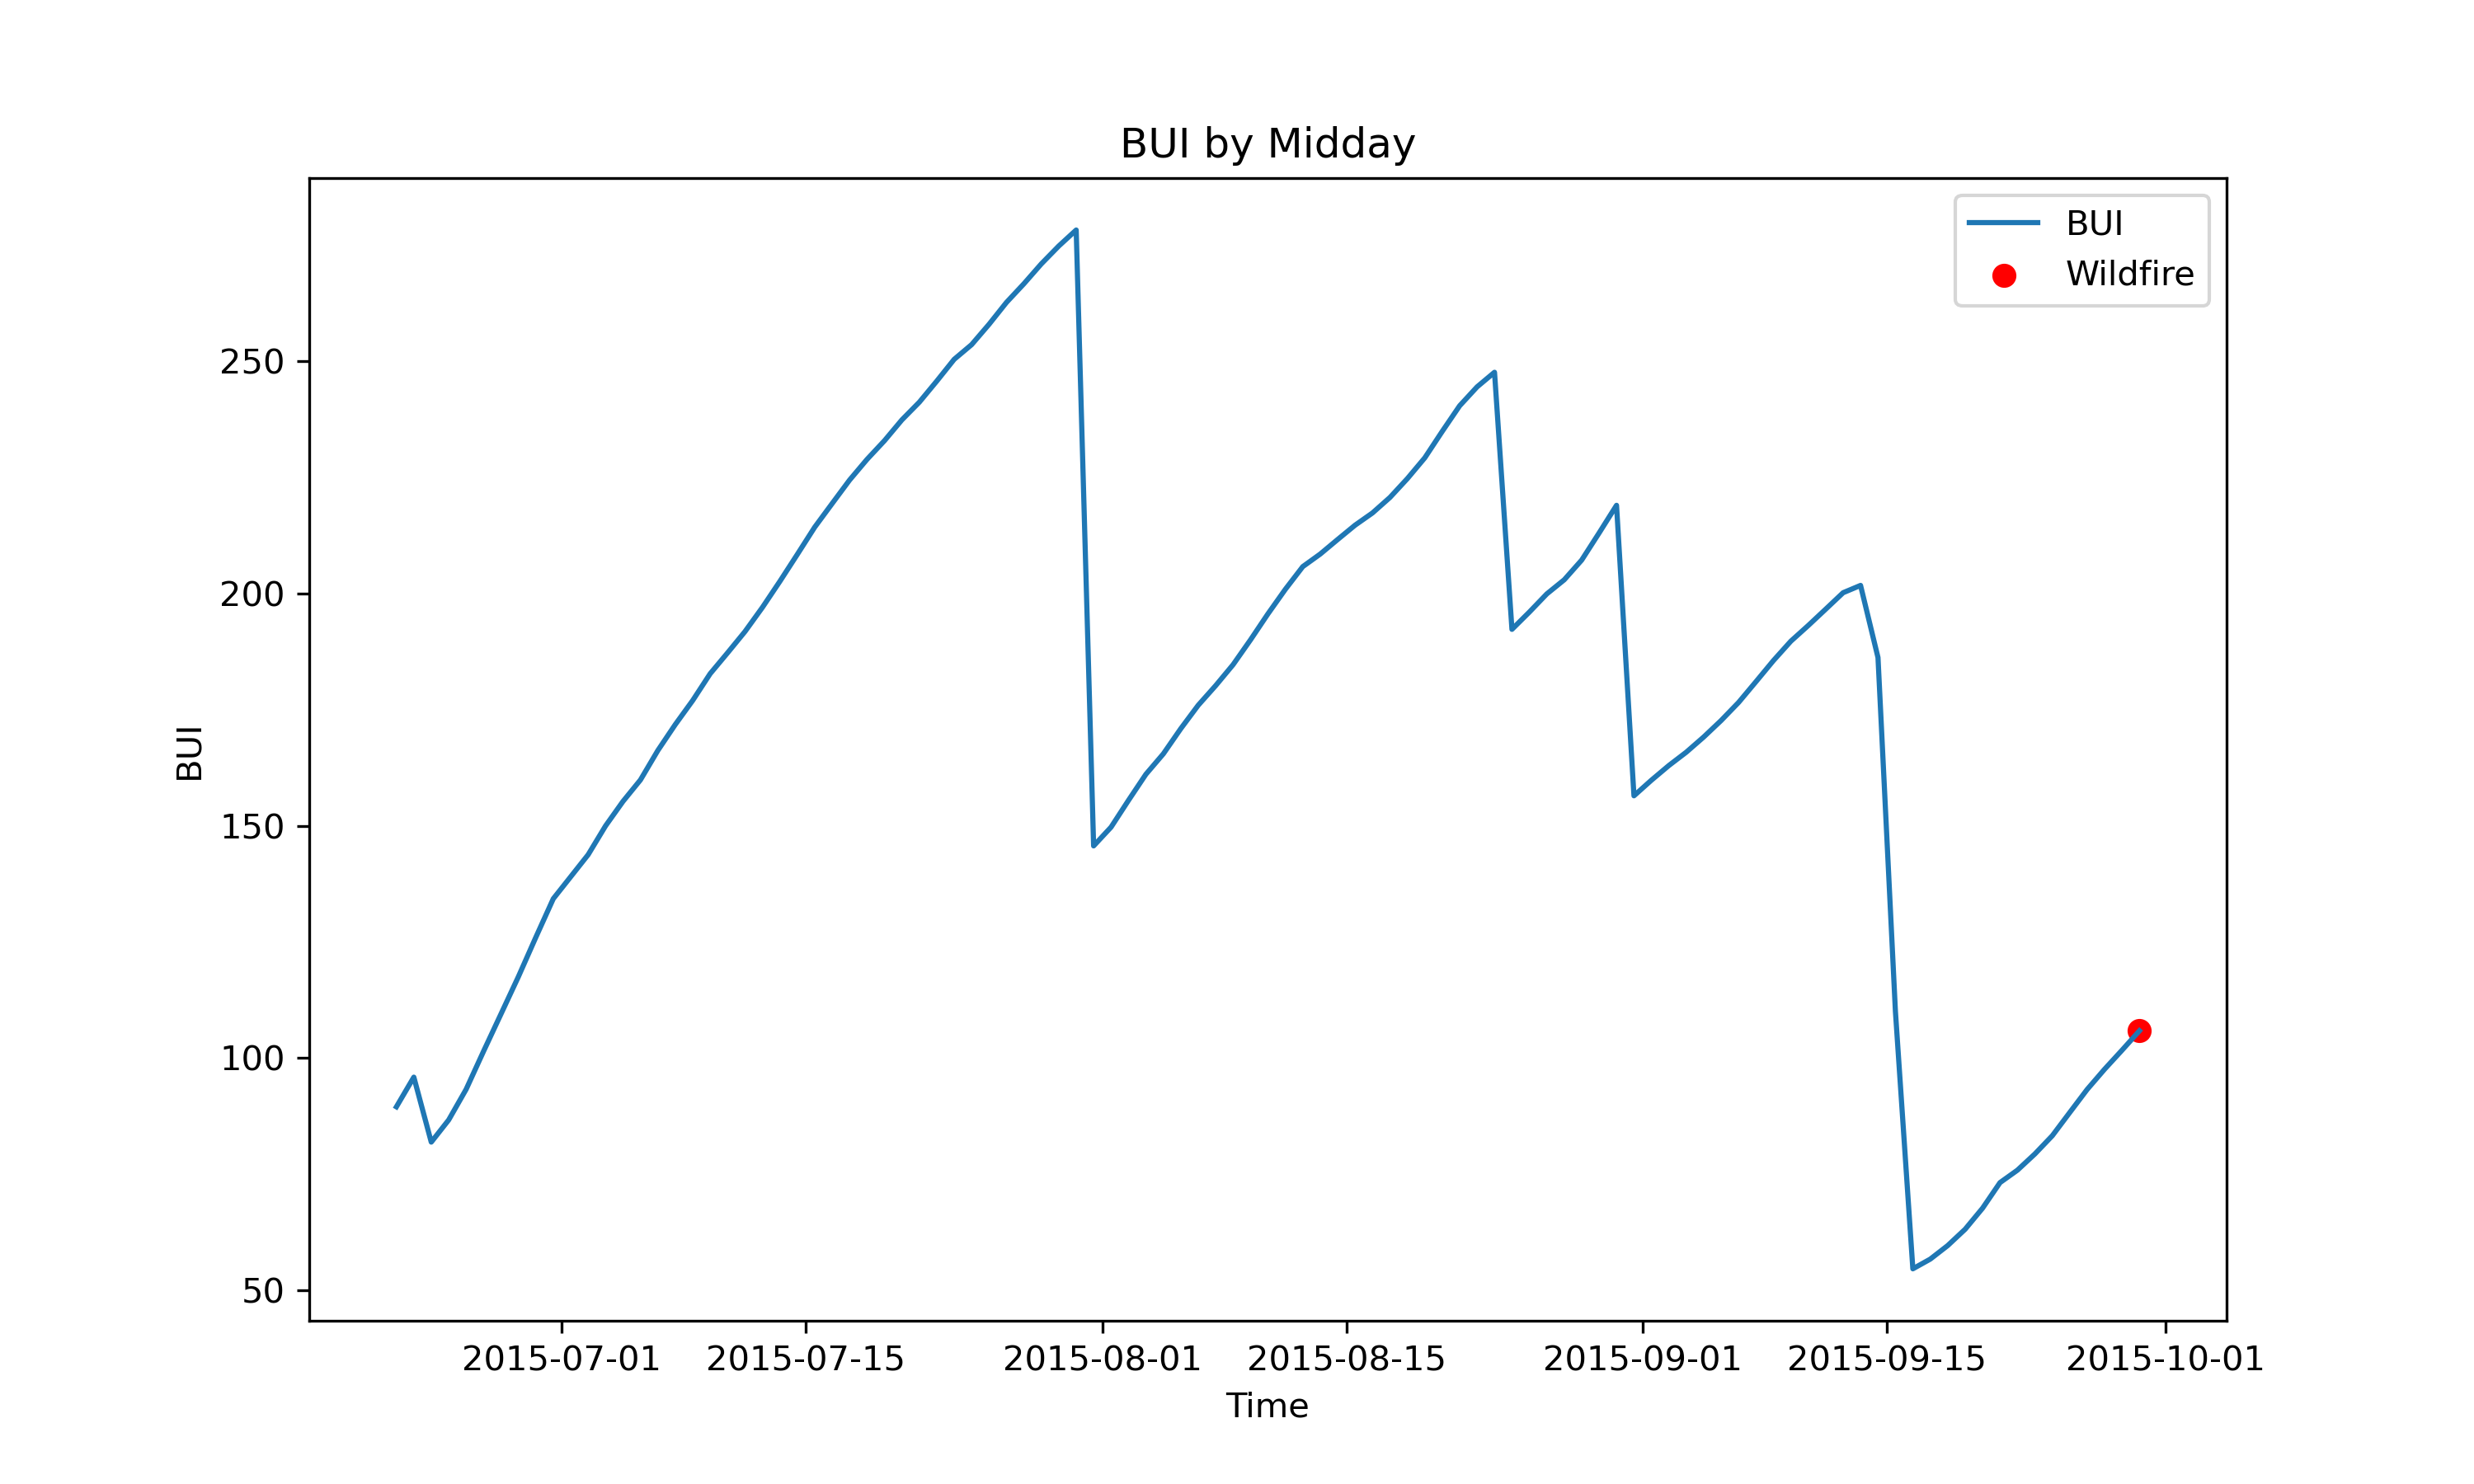
\includegraphics[width=\textwidth]{graphs/2015MesmoSitio/2015CalcBUI12.png}
        \caption{BUI - Calculated value}
        \label{fig:bui_calculated_2015_semfogo}
    \end{subfigure}
    \label{fig:comparison_bui_semfogo_copernicus_calculated}
\end{figure}

\FloatBarrier

\section{Comparison of Copernicus and Simulated FWI}

\subsection{Fogo de 2015}
\begin{figure}[h]
\caption{Comparison of FWI calculated values and Copernicus at midday}
    \centering
    \begin{subfigure}{0.49\textwidth}
        \centering
        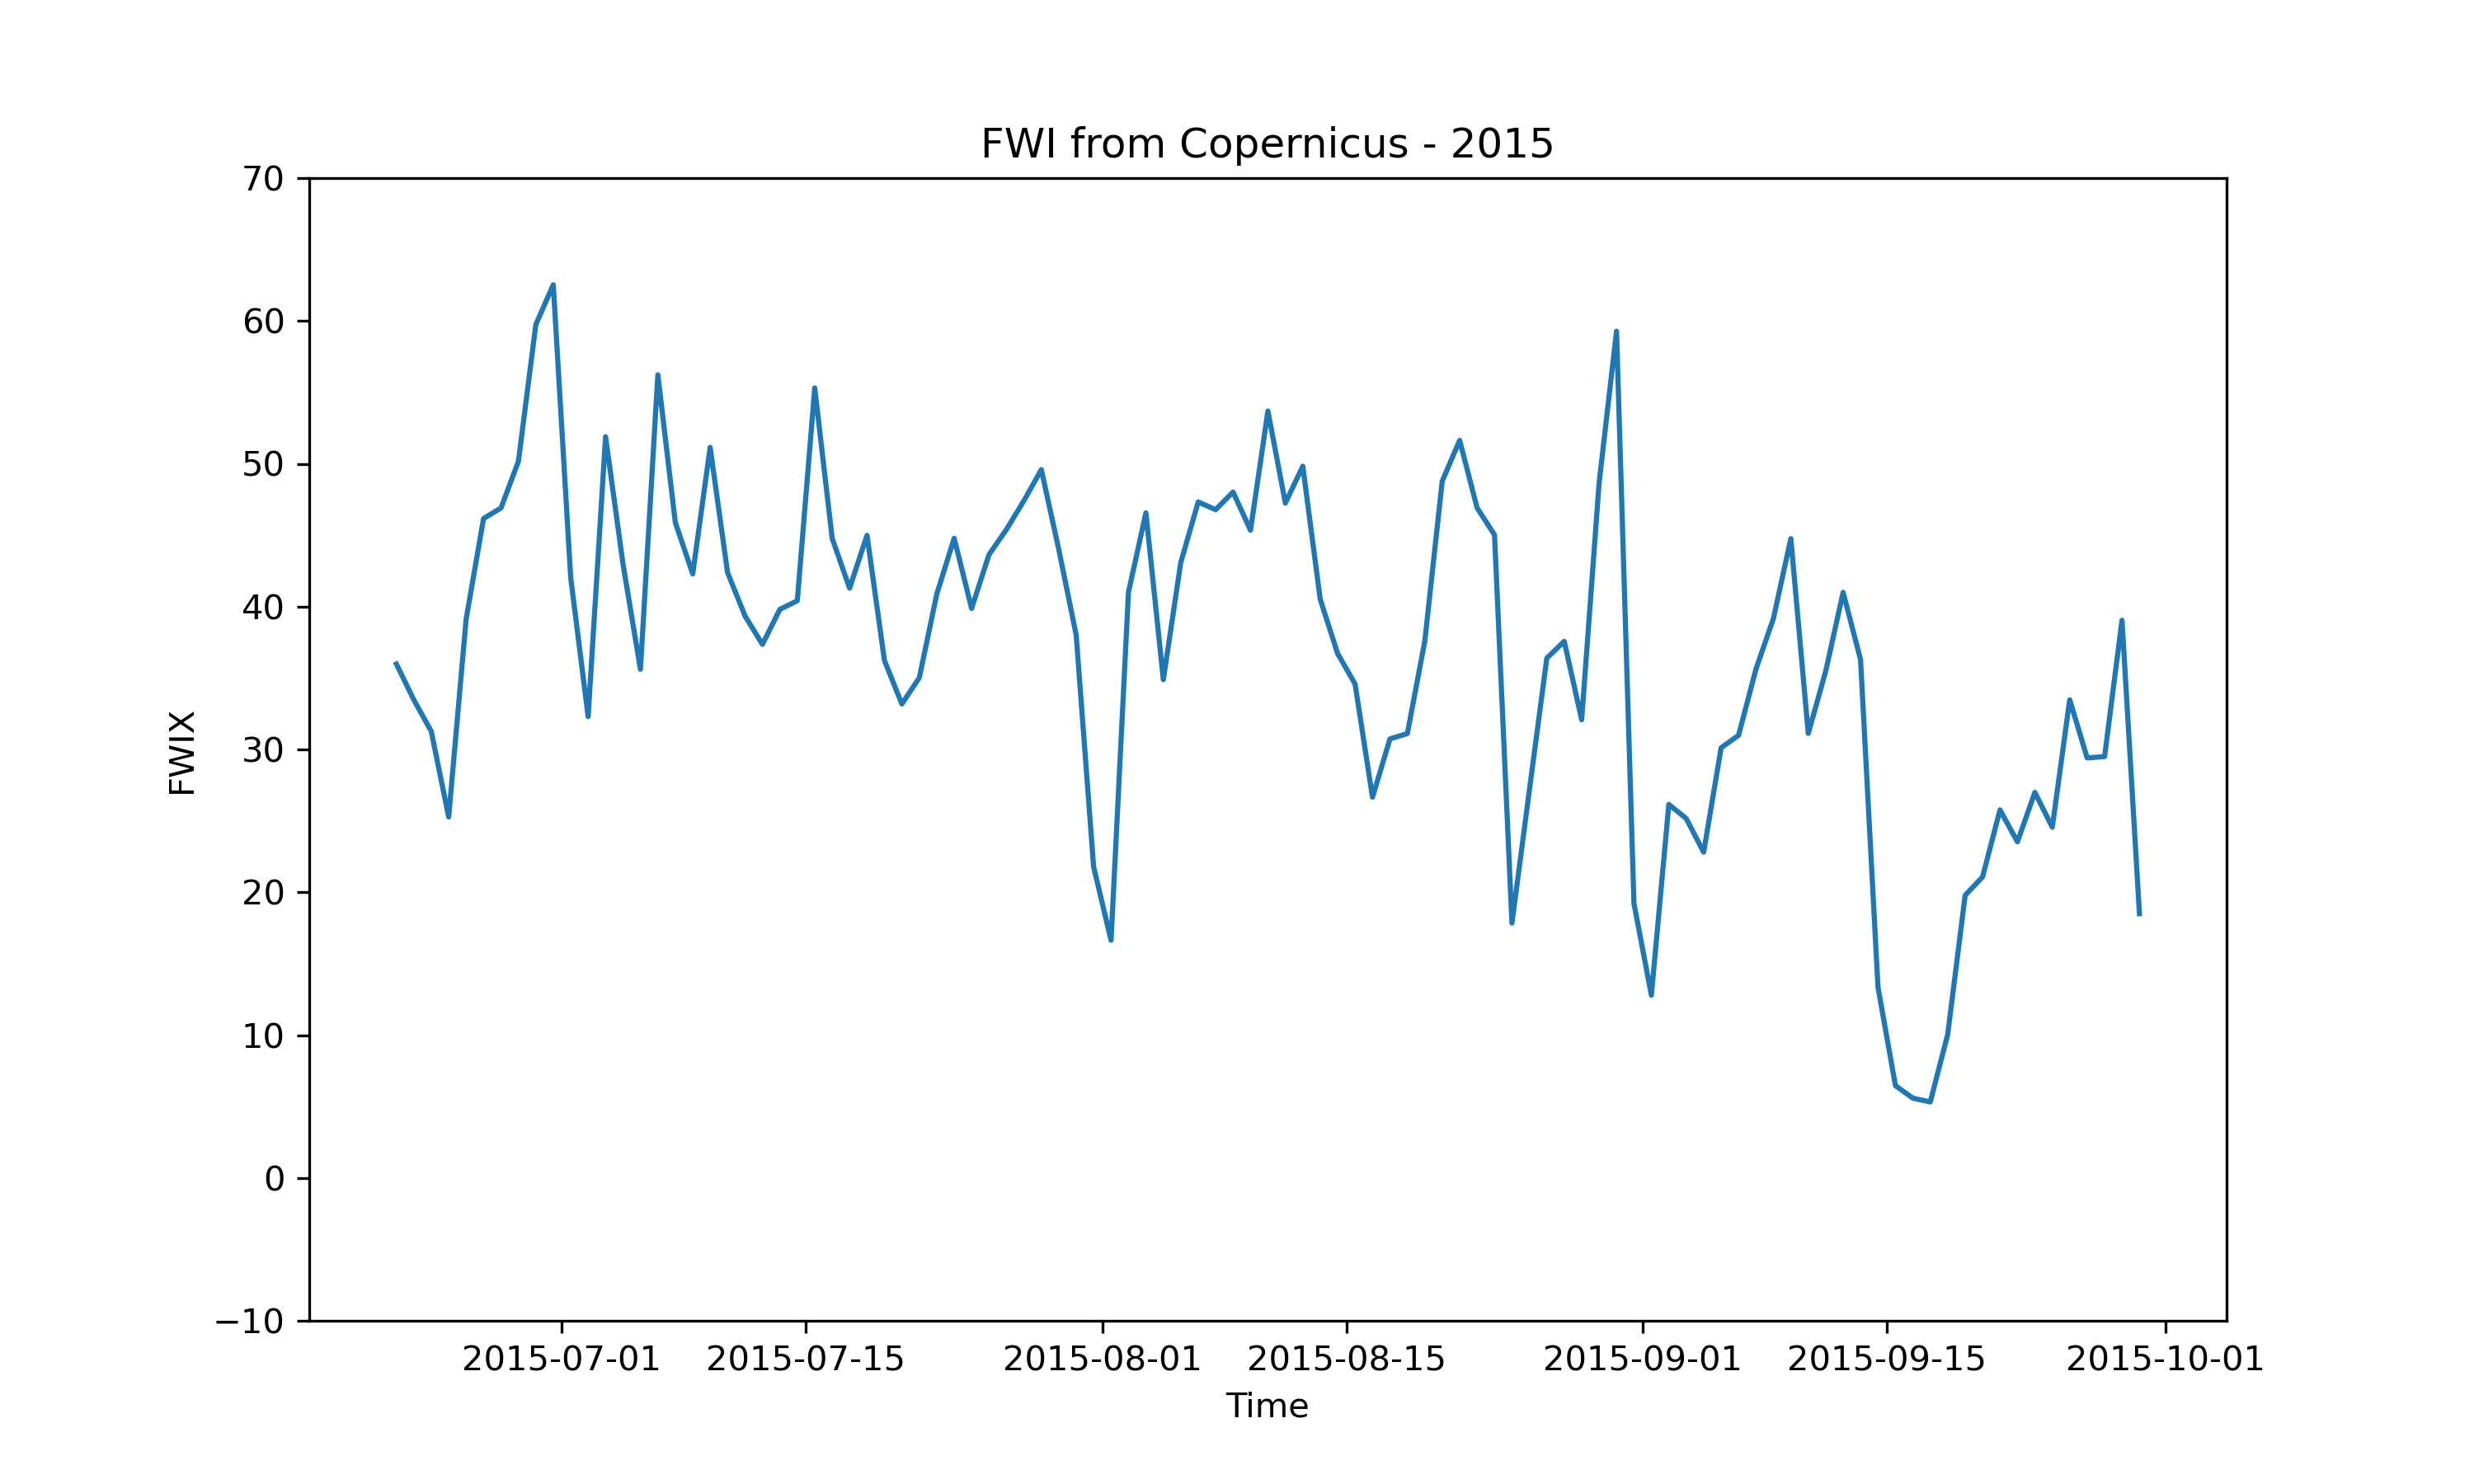
\includegraphics[width=\textwidth]{graphs/2015/2015CopernicusFWI12.png}
        \caption{FWI - Copernicus}
        \label{fig:fwi_copernicus_2015_midday}
    \end{subfigure}
    \hfill
    \begin{subfigure}{0.49\textwidth}
        \centering
        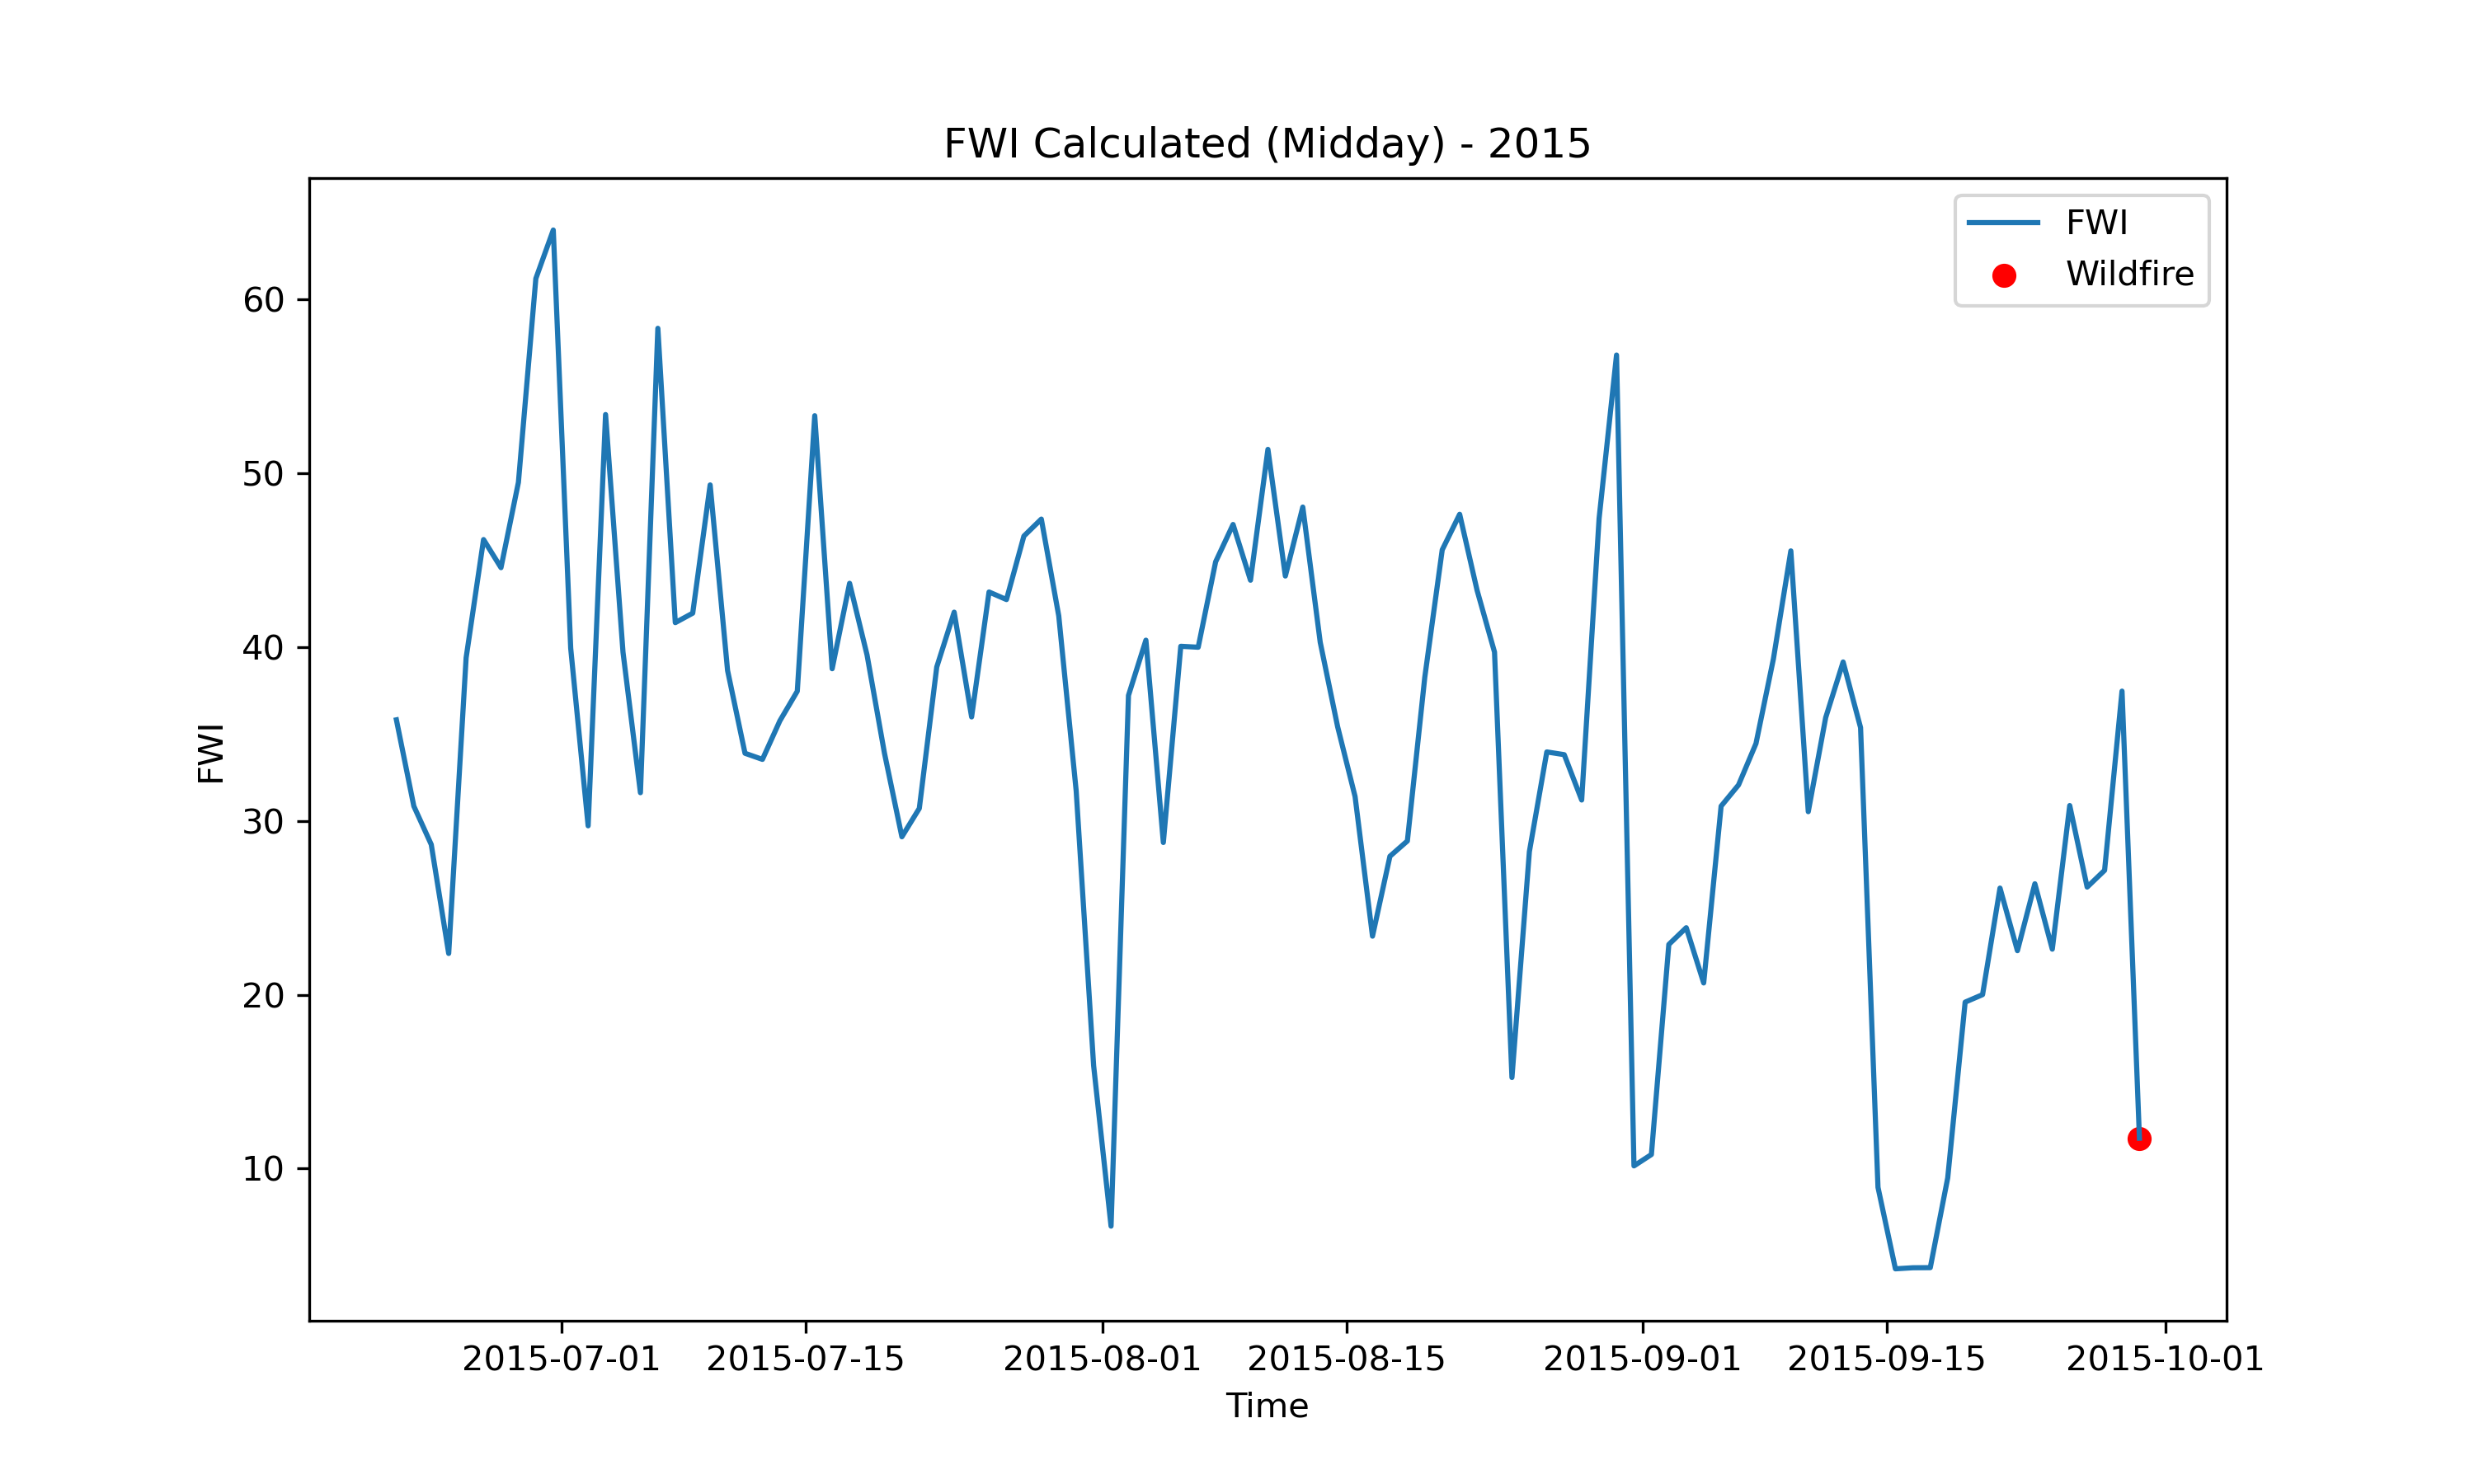
\includegraphics[width=\textwidth]{graphs/2015/2015CalcFWI12.png}
        \caption{FWI - Calculated value}
        \label{fig:fwi_calculated_2015_midday}
    \end{subfigure}
    \label{fig:comparison_fwi_midday_copernicus_calculated}
\end{figure}

\begin{figure}[h]
\caption{Comparison of FFMC calculated values and Copernicus at midday}
    \centering
    \begin{subfigure}{0.49\textwidth}
        \centering
        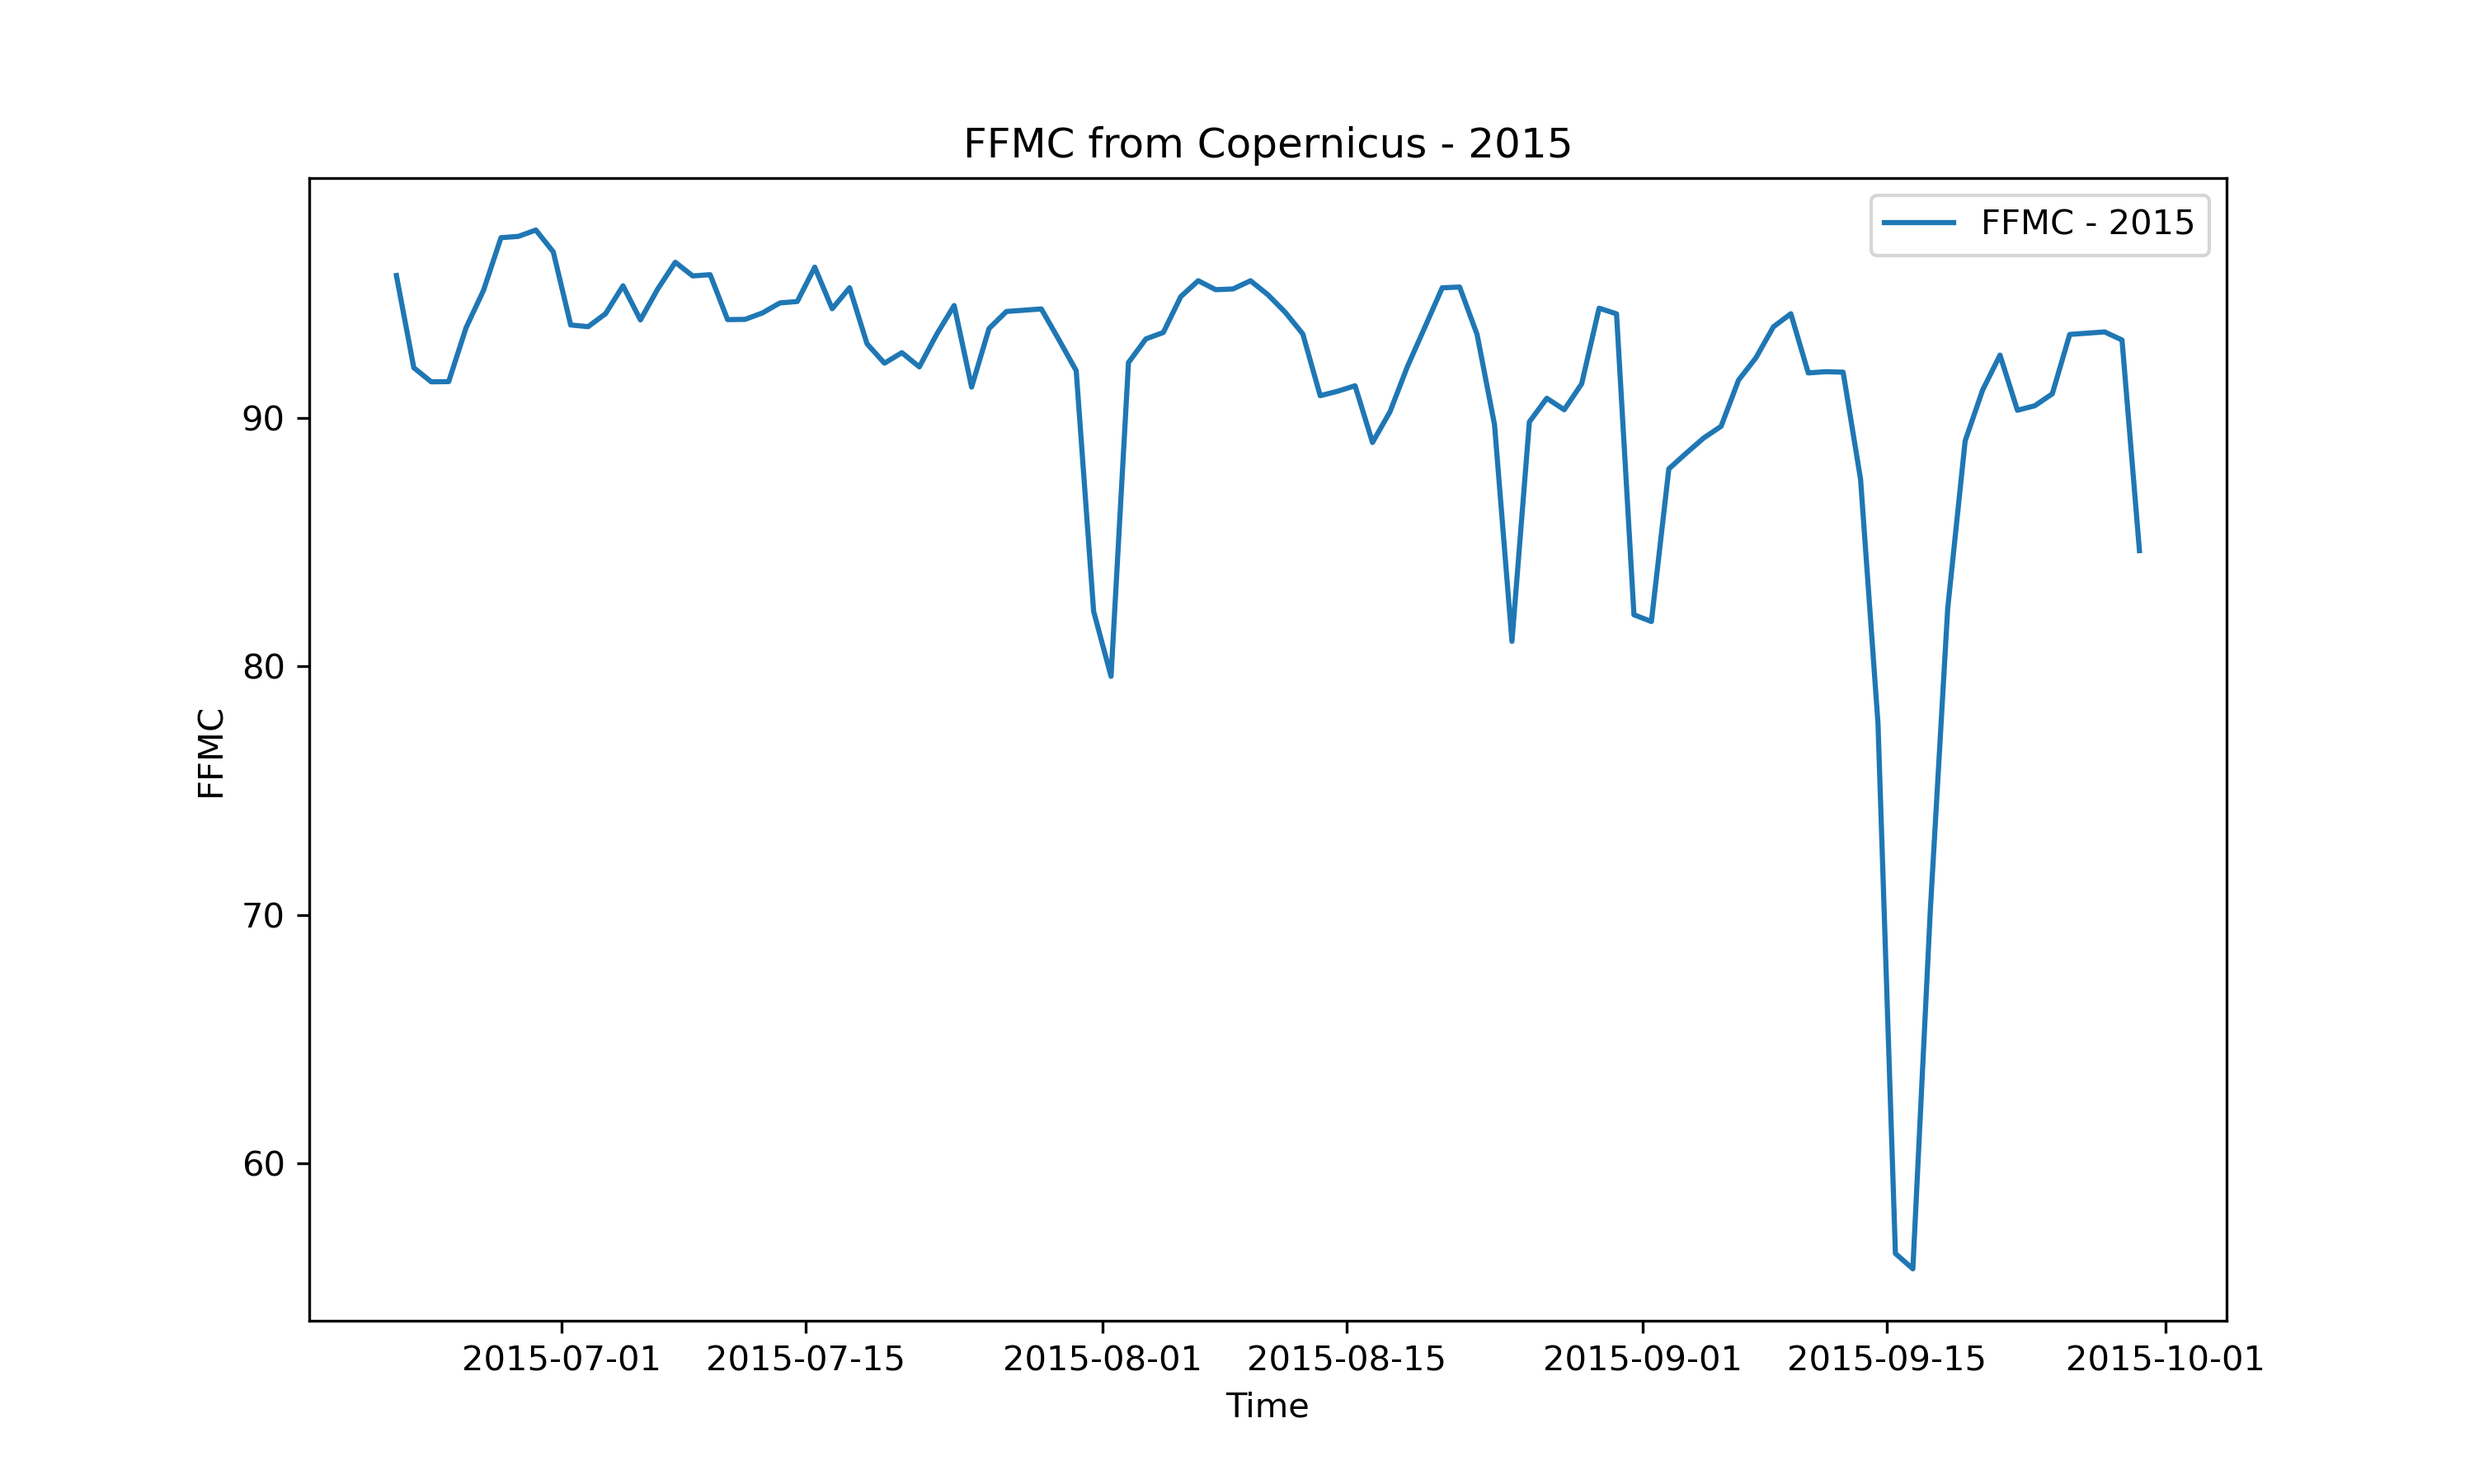
\includegraphics[width=\textwidth]{graphs/2015/2015CopernicusFFMC12.png}
        \caption{FFMC - Copernicus}
        \label{fig:ffmc_copernicus_2015_midday}
    \end{subfigure}
    \hfill
    \begin{subfigure}{0.49\textwidth}
        \centering
        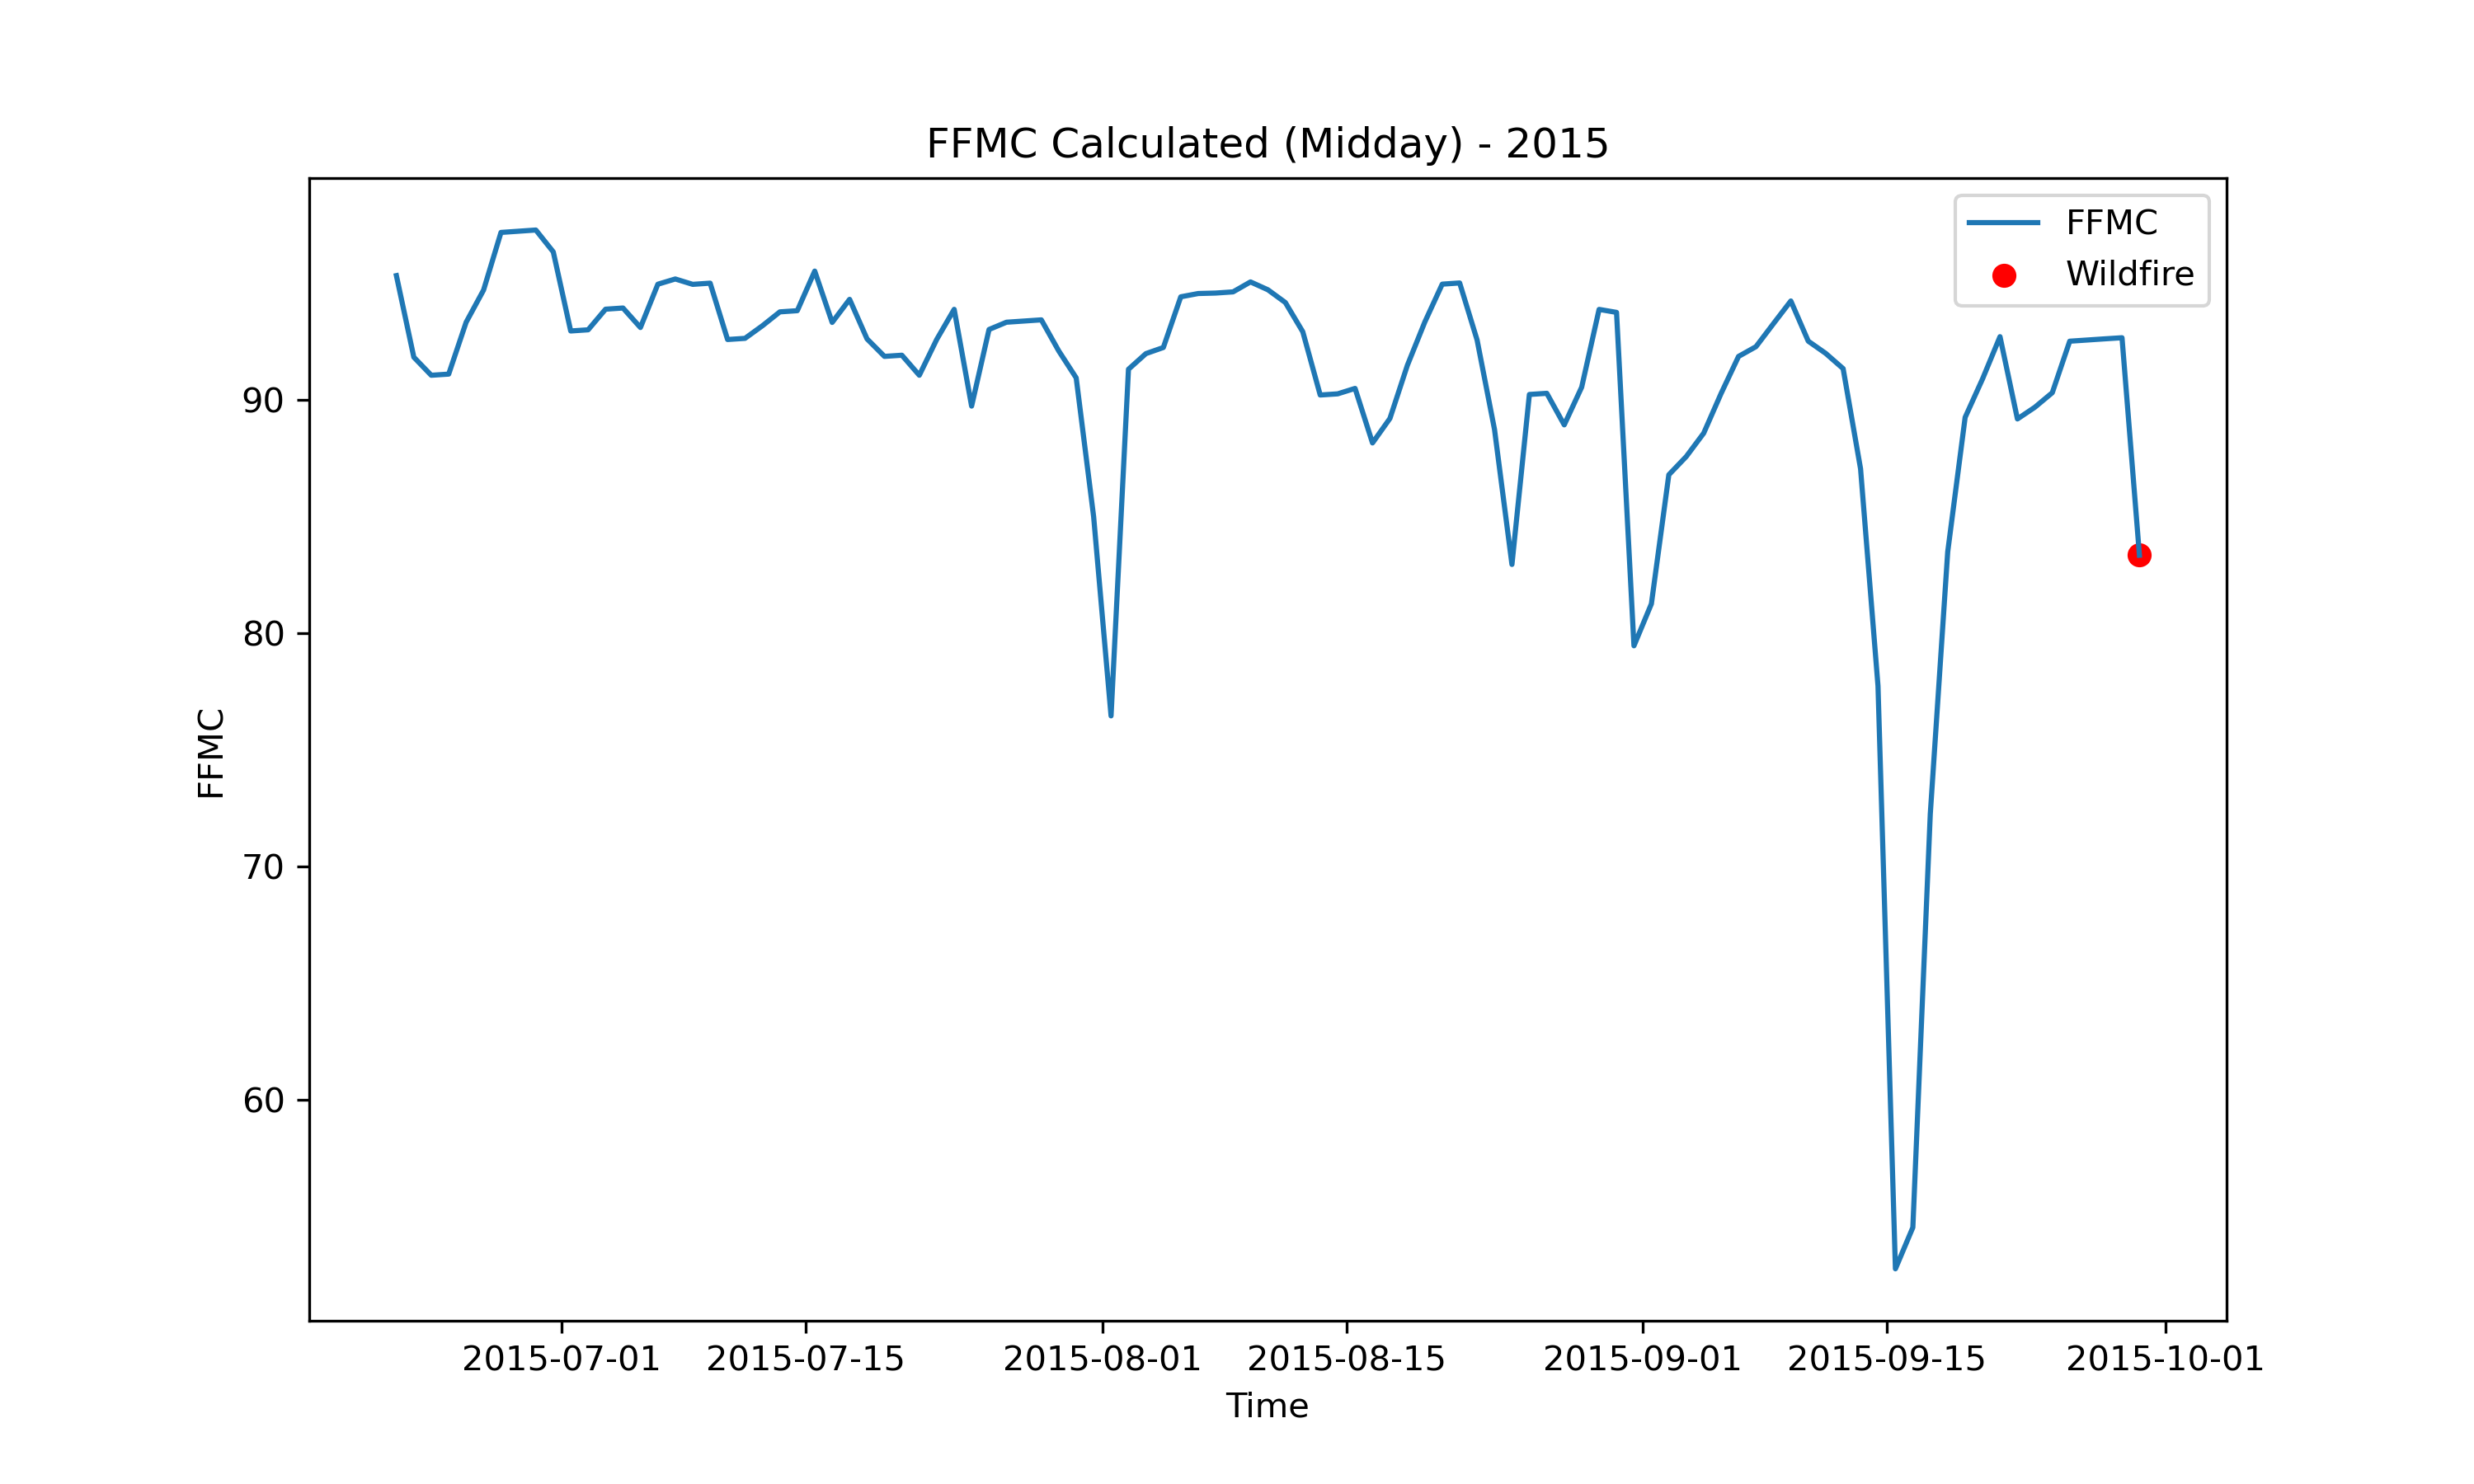
\includegraphics[width=\textwidth]{graphs/2015/2015CalcFFMC12.png}
        \caption{FFMC - Calculated value}
        \label{fig:ffmc_calculated_2015_midday}
    \end{subfigure}
    \label{fig:comparison_ffmc_midday_copernicus_calculated}
\end{figure}

\begin{figure}[h]
\caption{Comparison of DMC calculated values and Copernicus at midday}
    \centering
    \begin{subfigure}{0.49\textwidth}
        \centering
        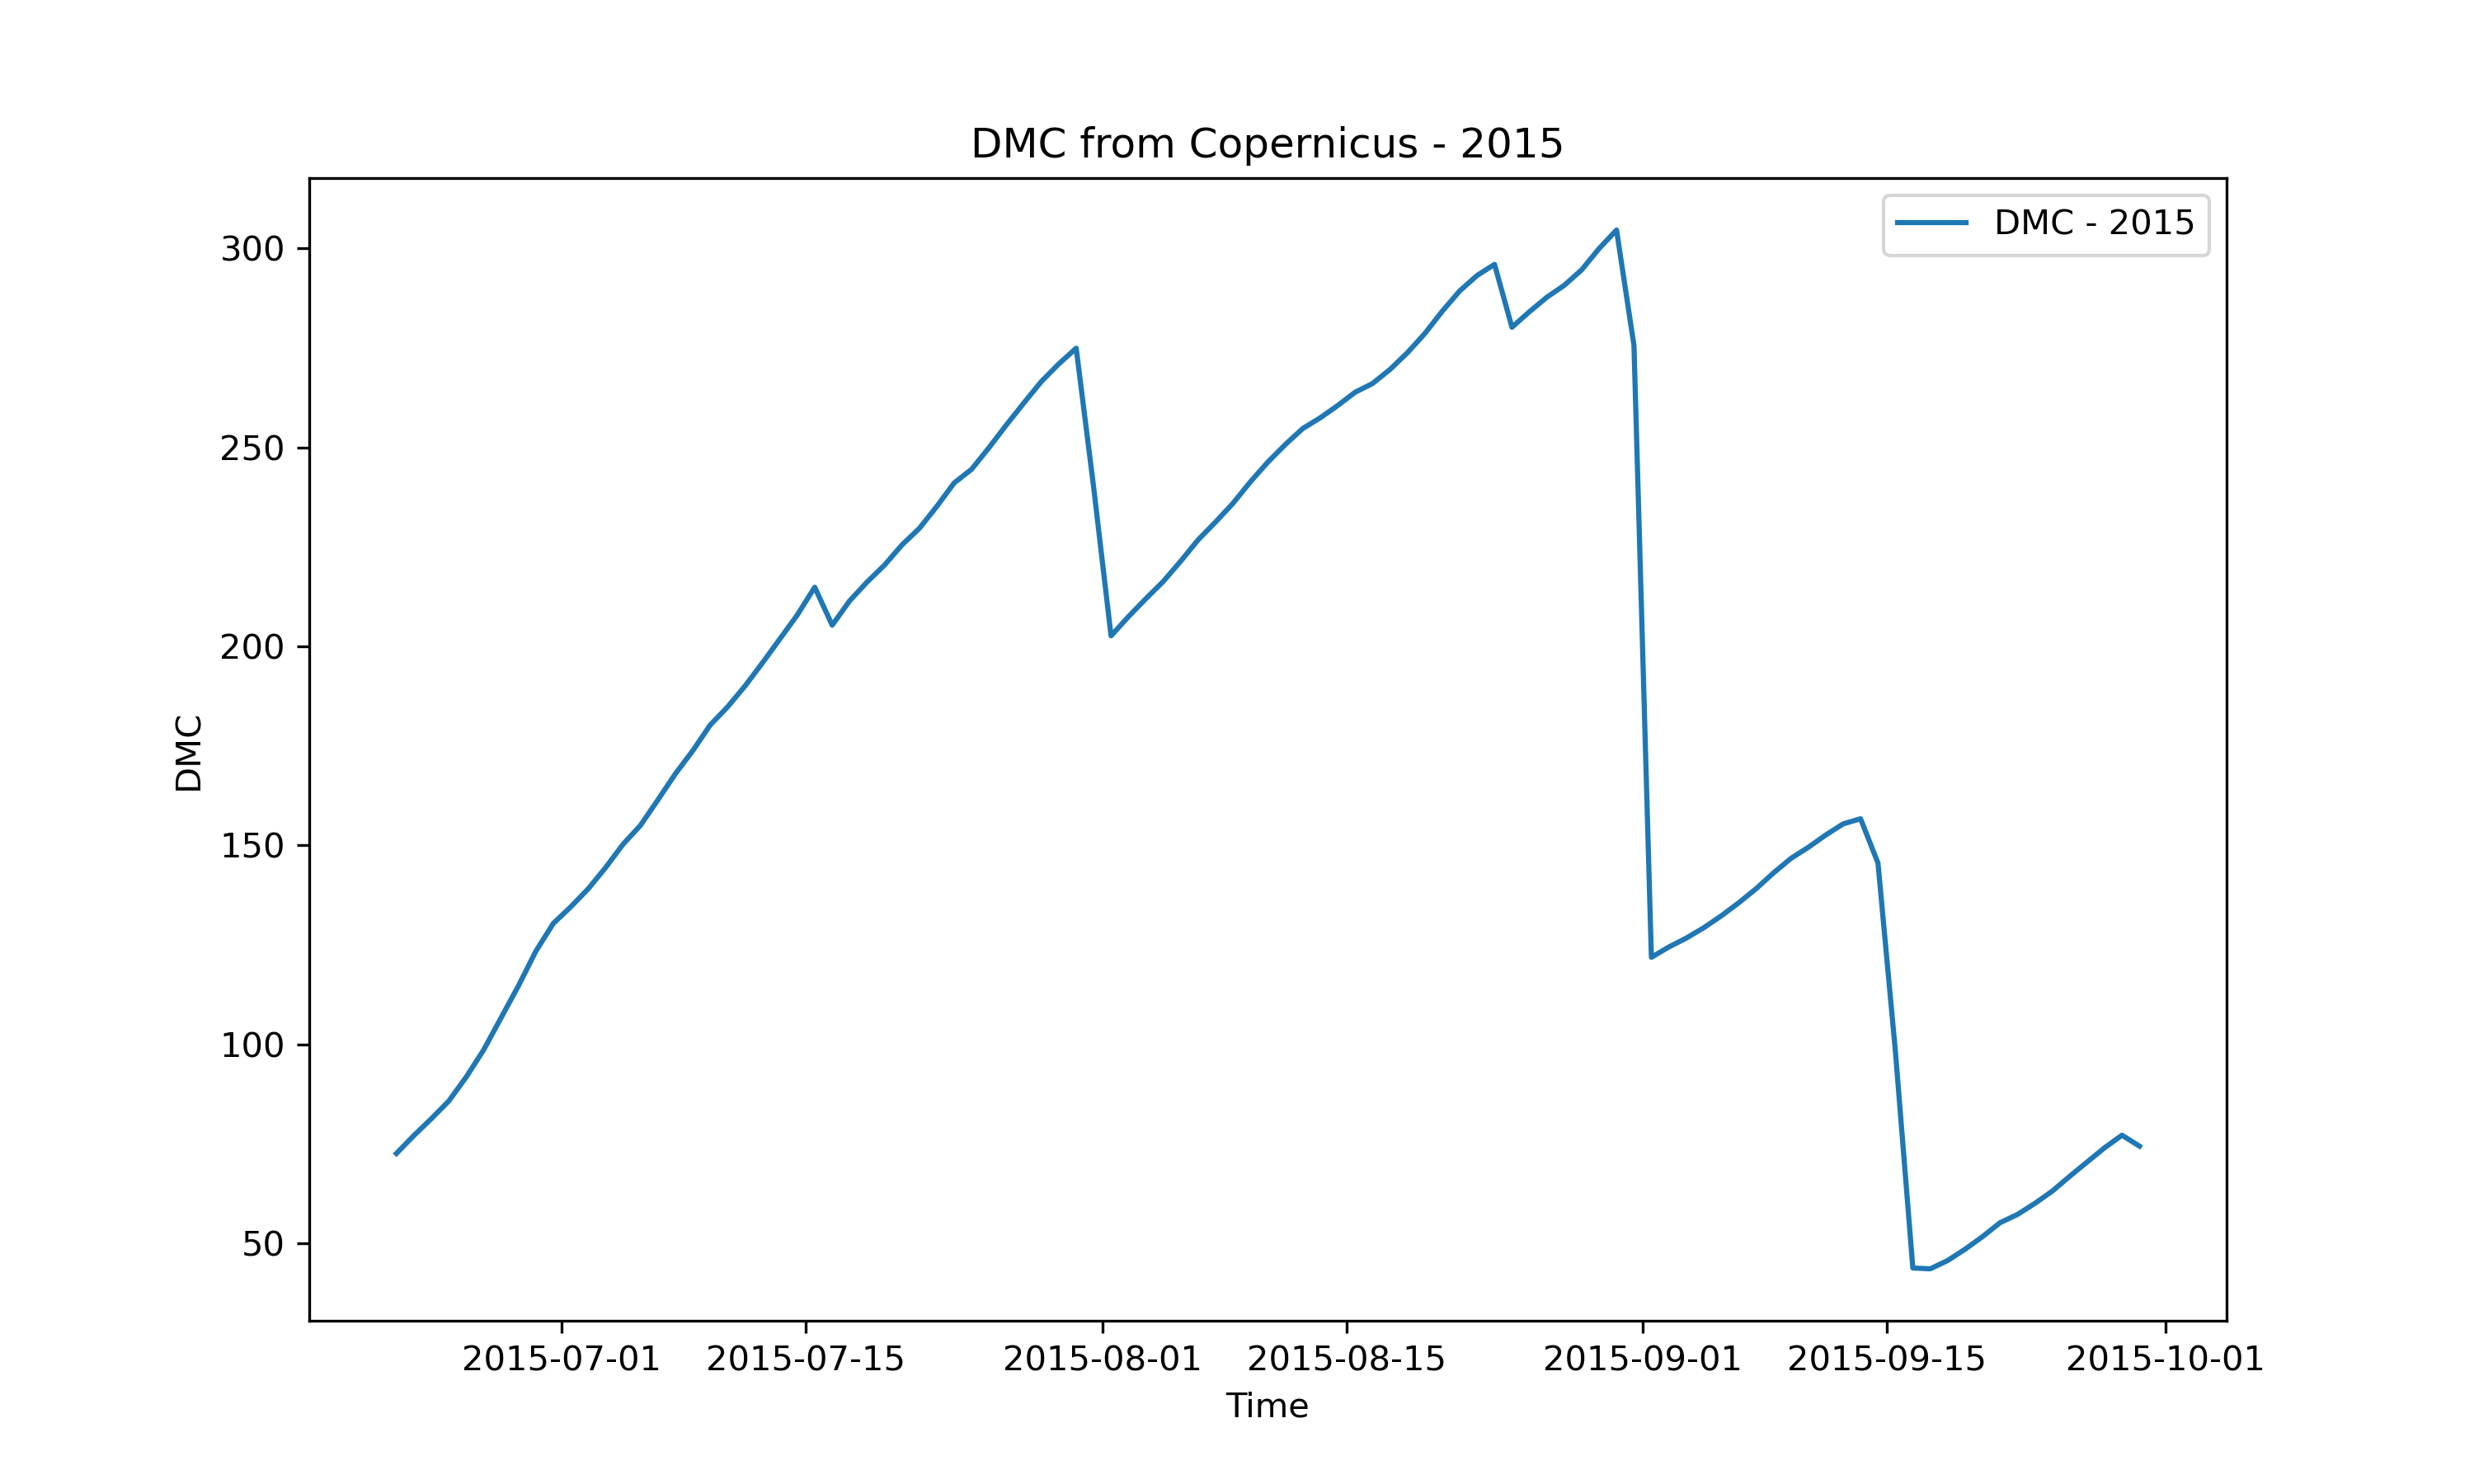
\includegraphics[width=\textwidth]{graphs/2015/2015CopernicusDMC12.png}
        \caption{DMC - Copernicus}
        \label{fig:dmc_copernicus_2015_midday}
    \end{subfigure}
    \hfill
    \begin{subfigure}{0.49\textwidth}
        \centering
        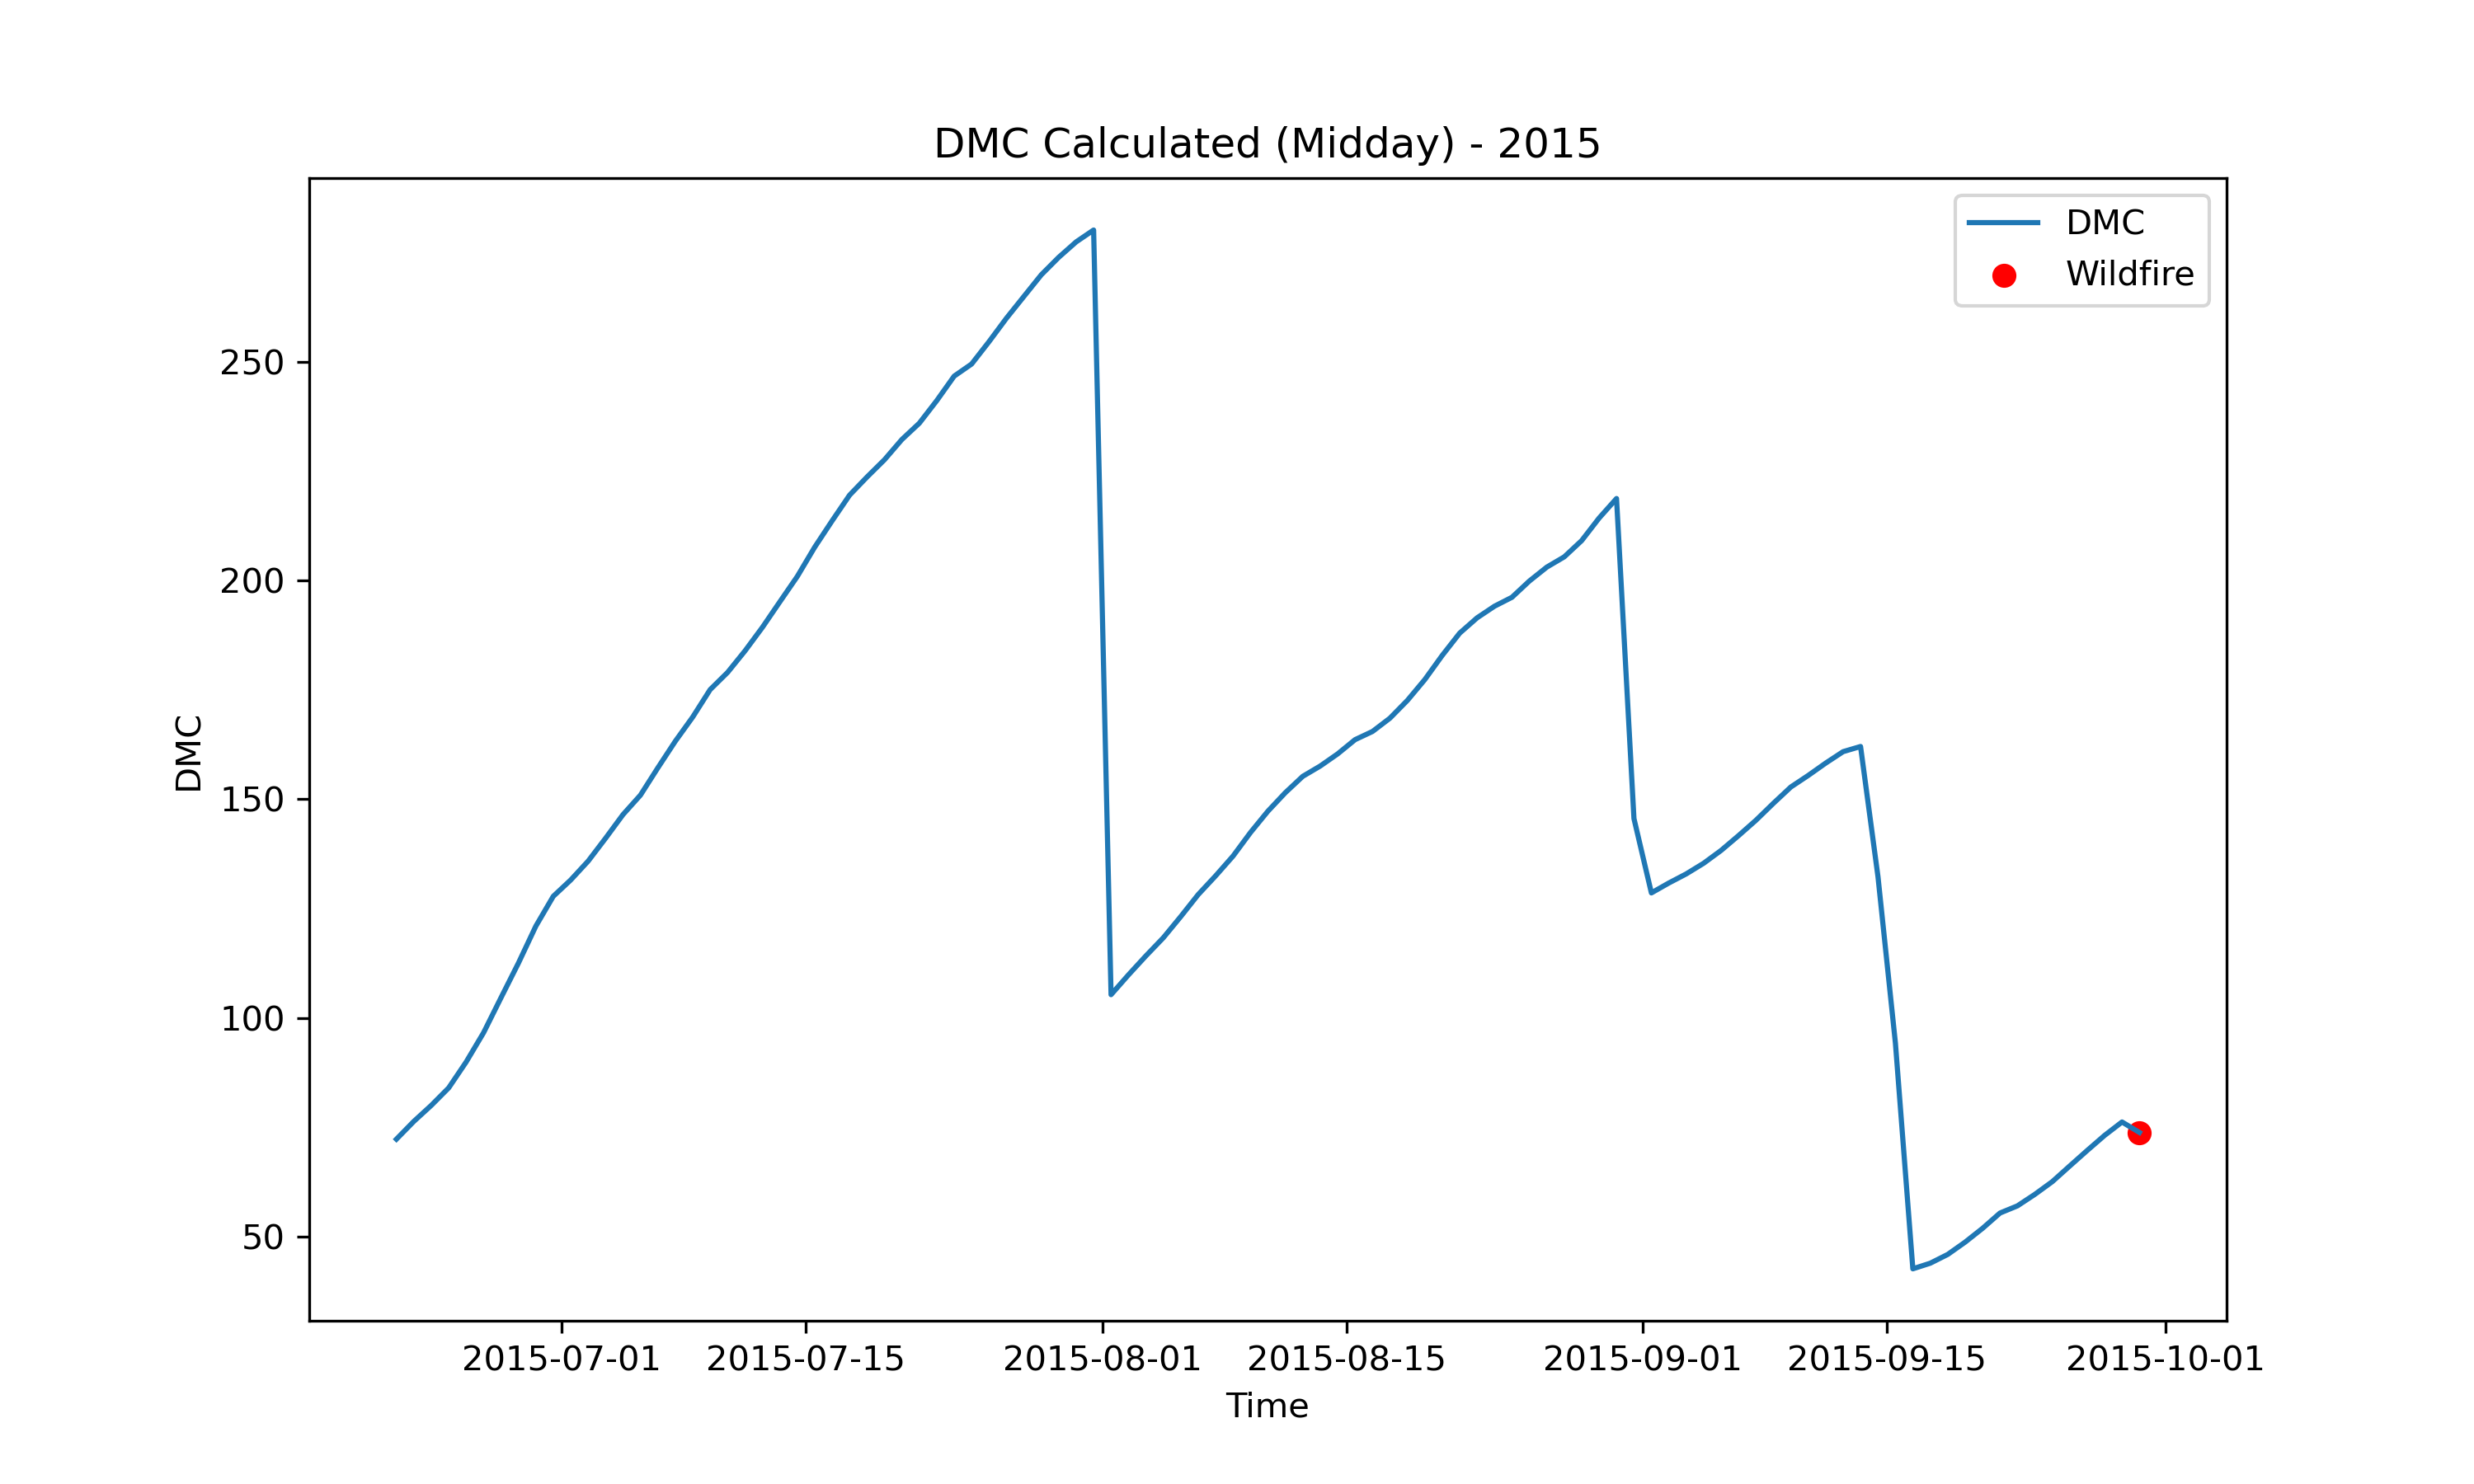
\includegraphics[width=\textwidth]{graphs/2015/2015CalcDMC12.png}
        \caption{DMC - Calculated value}
        \label{fig:dmc_calculated_2015_midday}
    \end{subfigure}
    \label{fig:comparison_dmc_midday_copernicus_calculated}
\end{figure}

\begin{figure}[h]
\caption{Comparison of DC calculated values and Copernicus at midday}
    \centering
    \begin{subfigure}{0.49\textwidth}
        \centering
        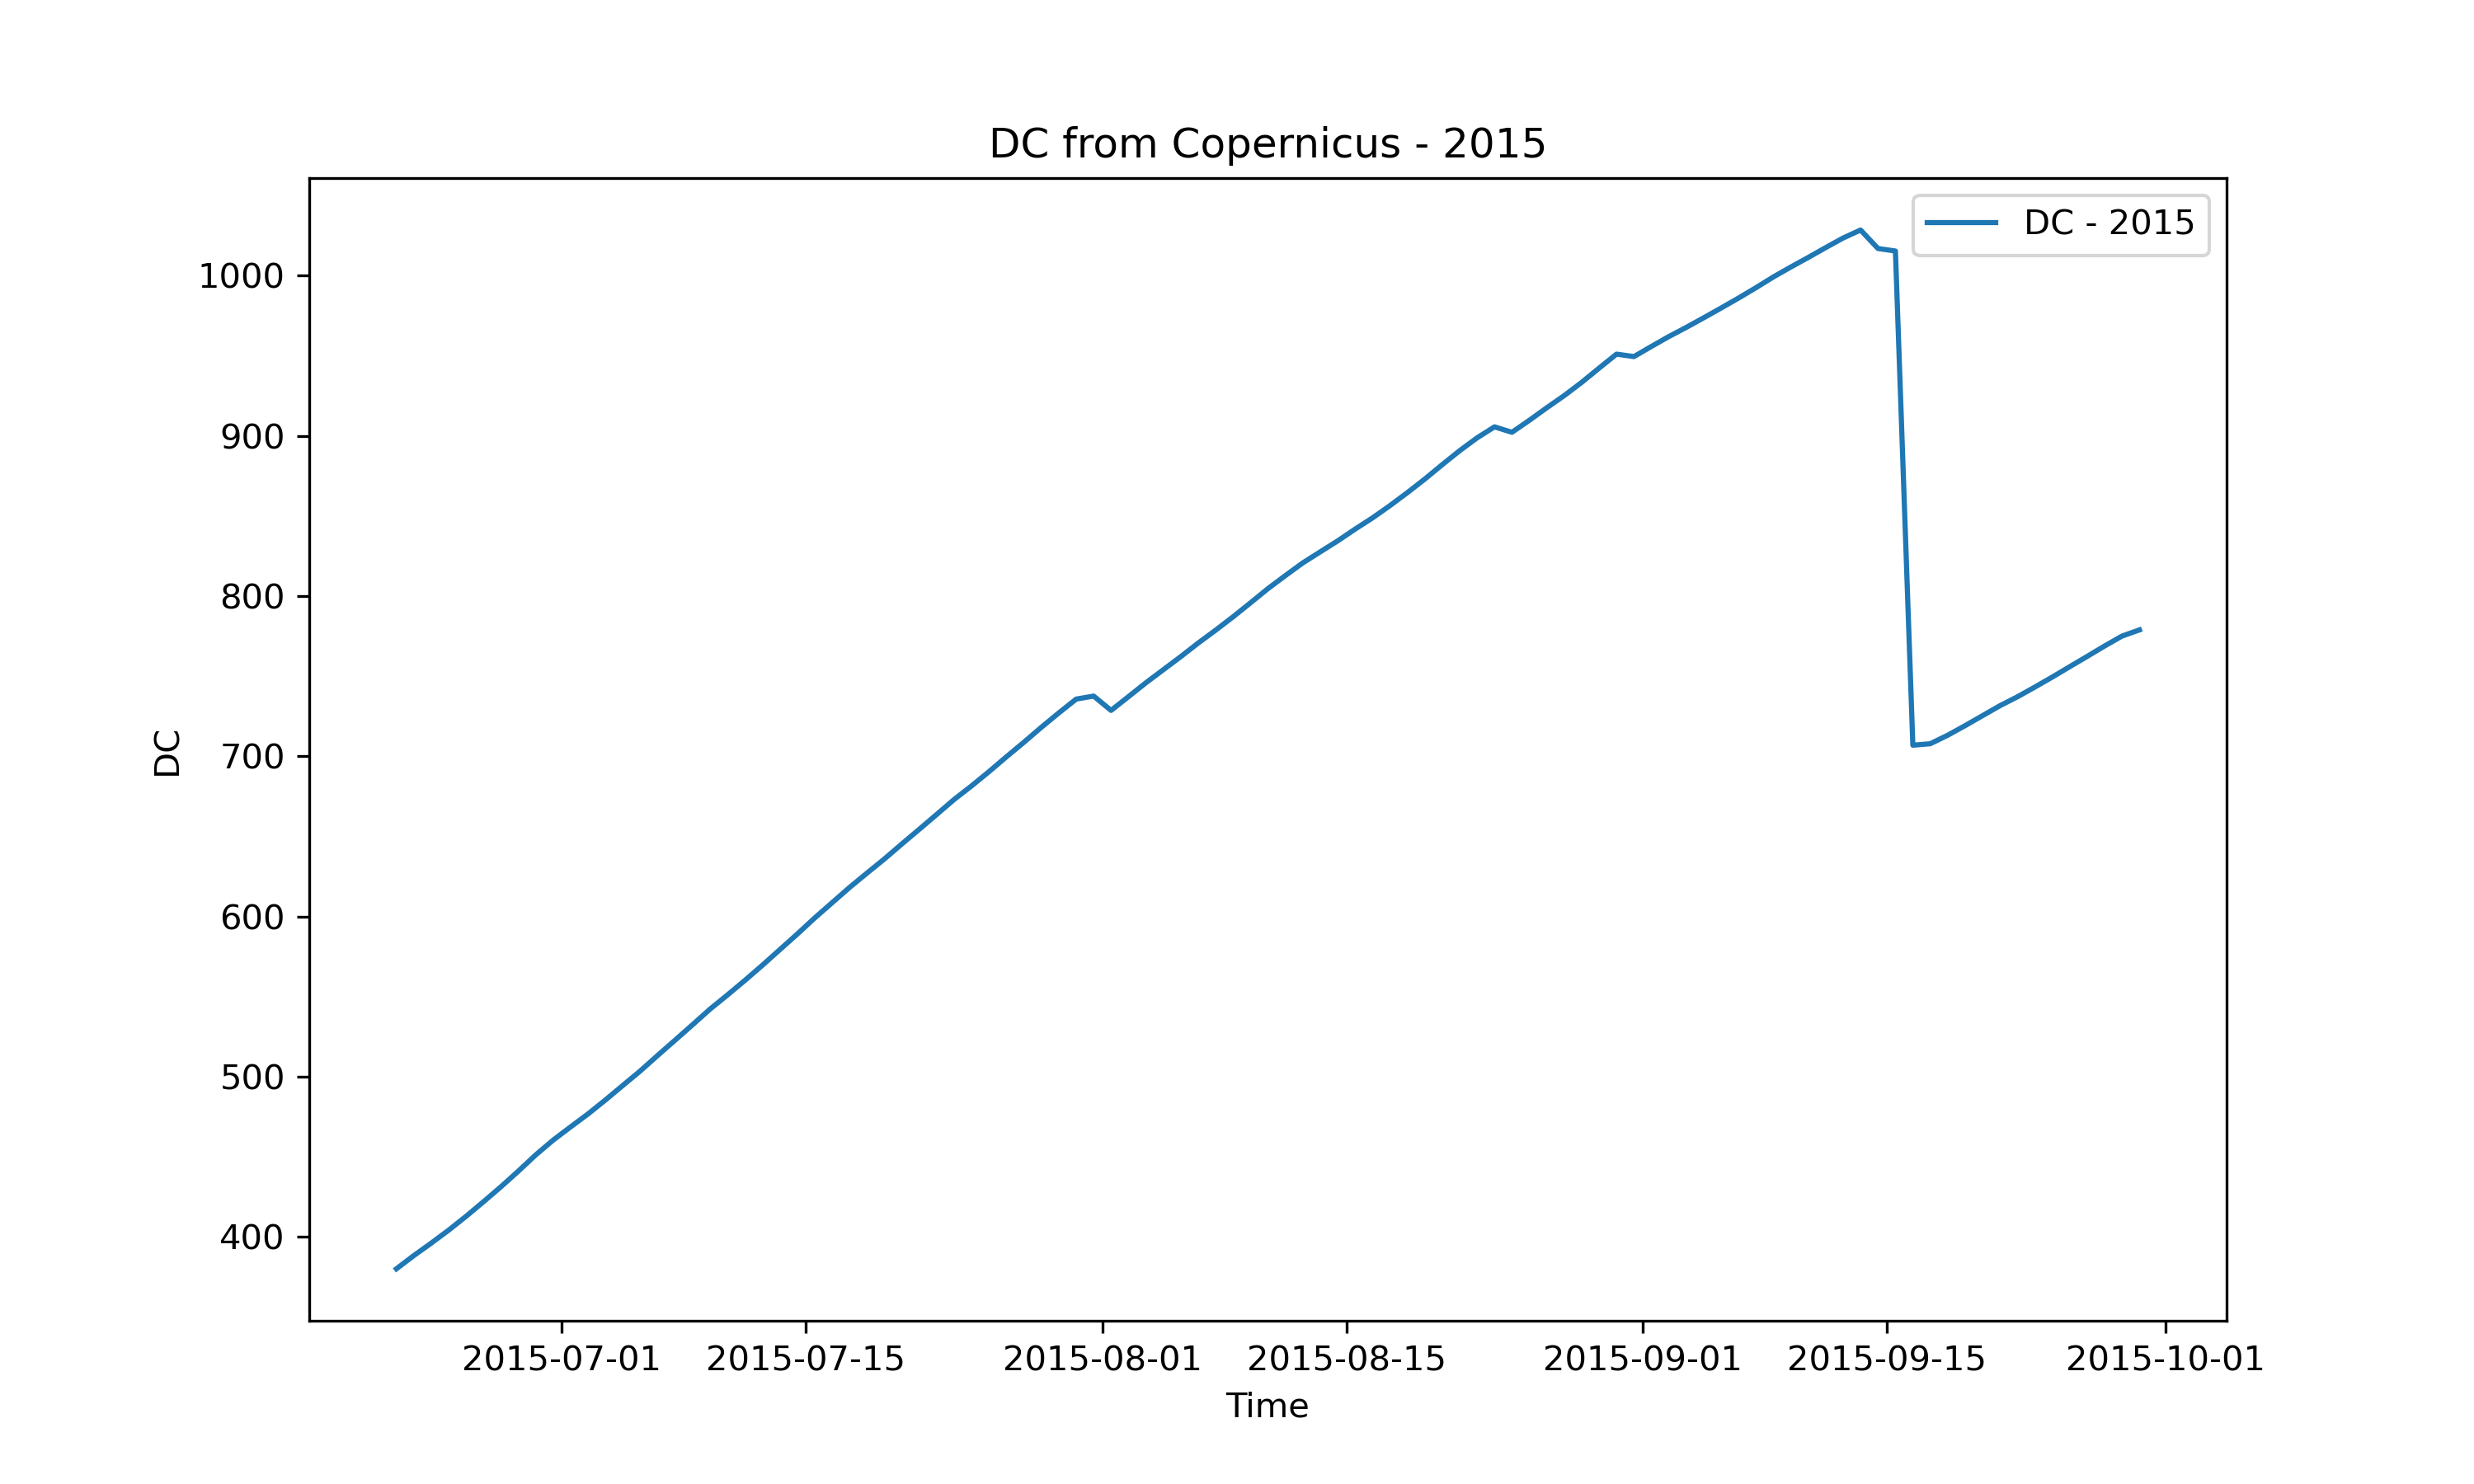
\includegraphics[width=\textwidth]{graphs/2015/2015CopernicusDC12.png}
        \caption{DC - Copernicus}
        \label{fig:dc_copernicus_2015_midday}
    \end{subfigure}
    \hfill
    \begin{subfigure}{0.49\textwidth}
        \centering
        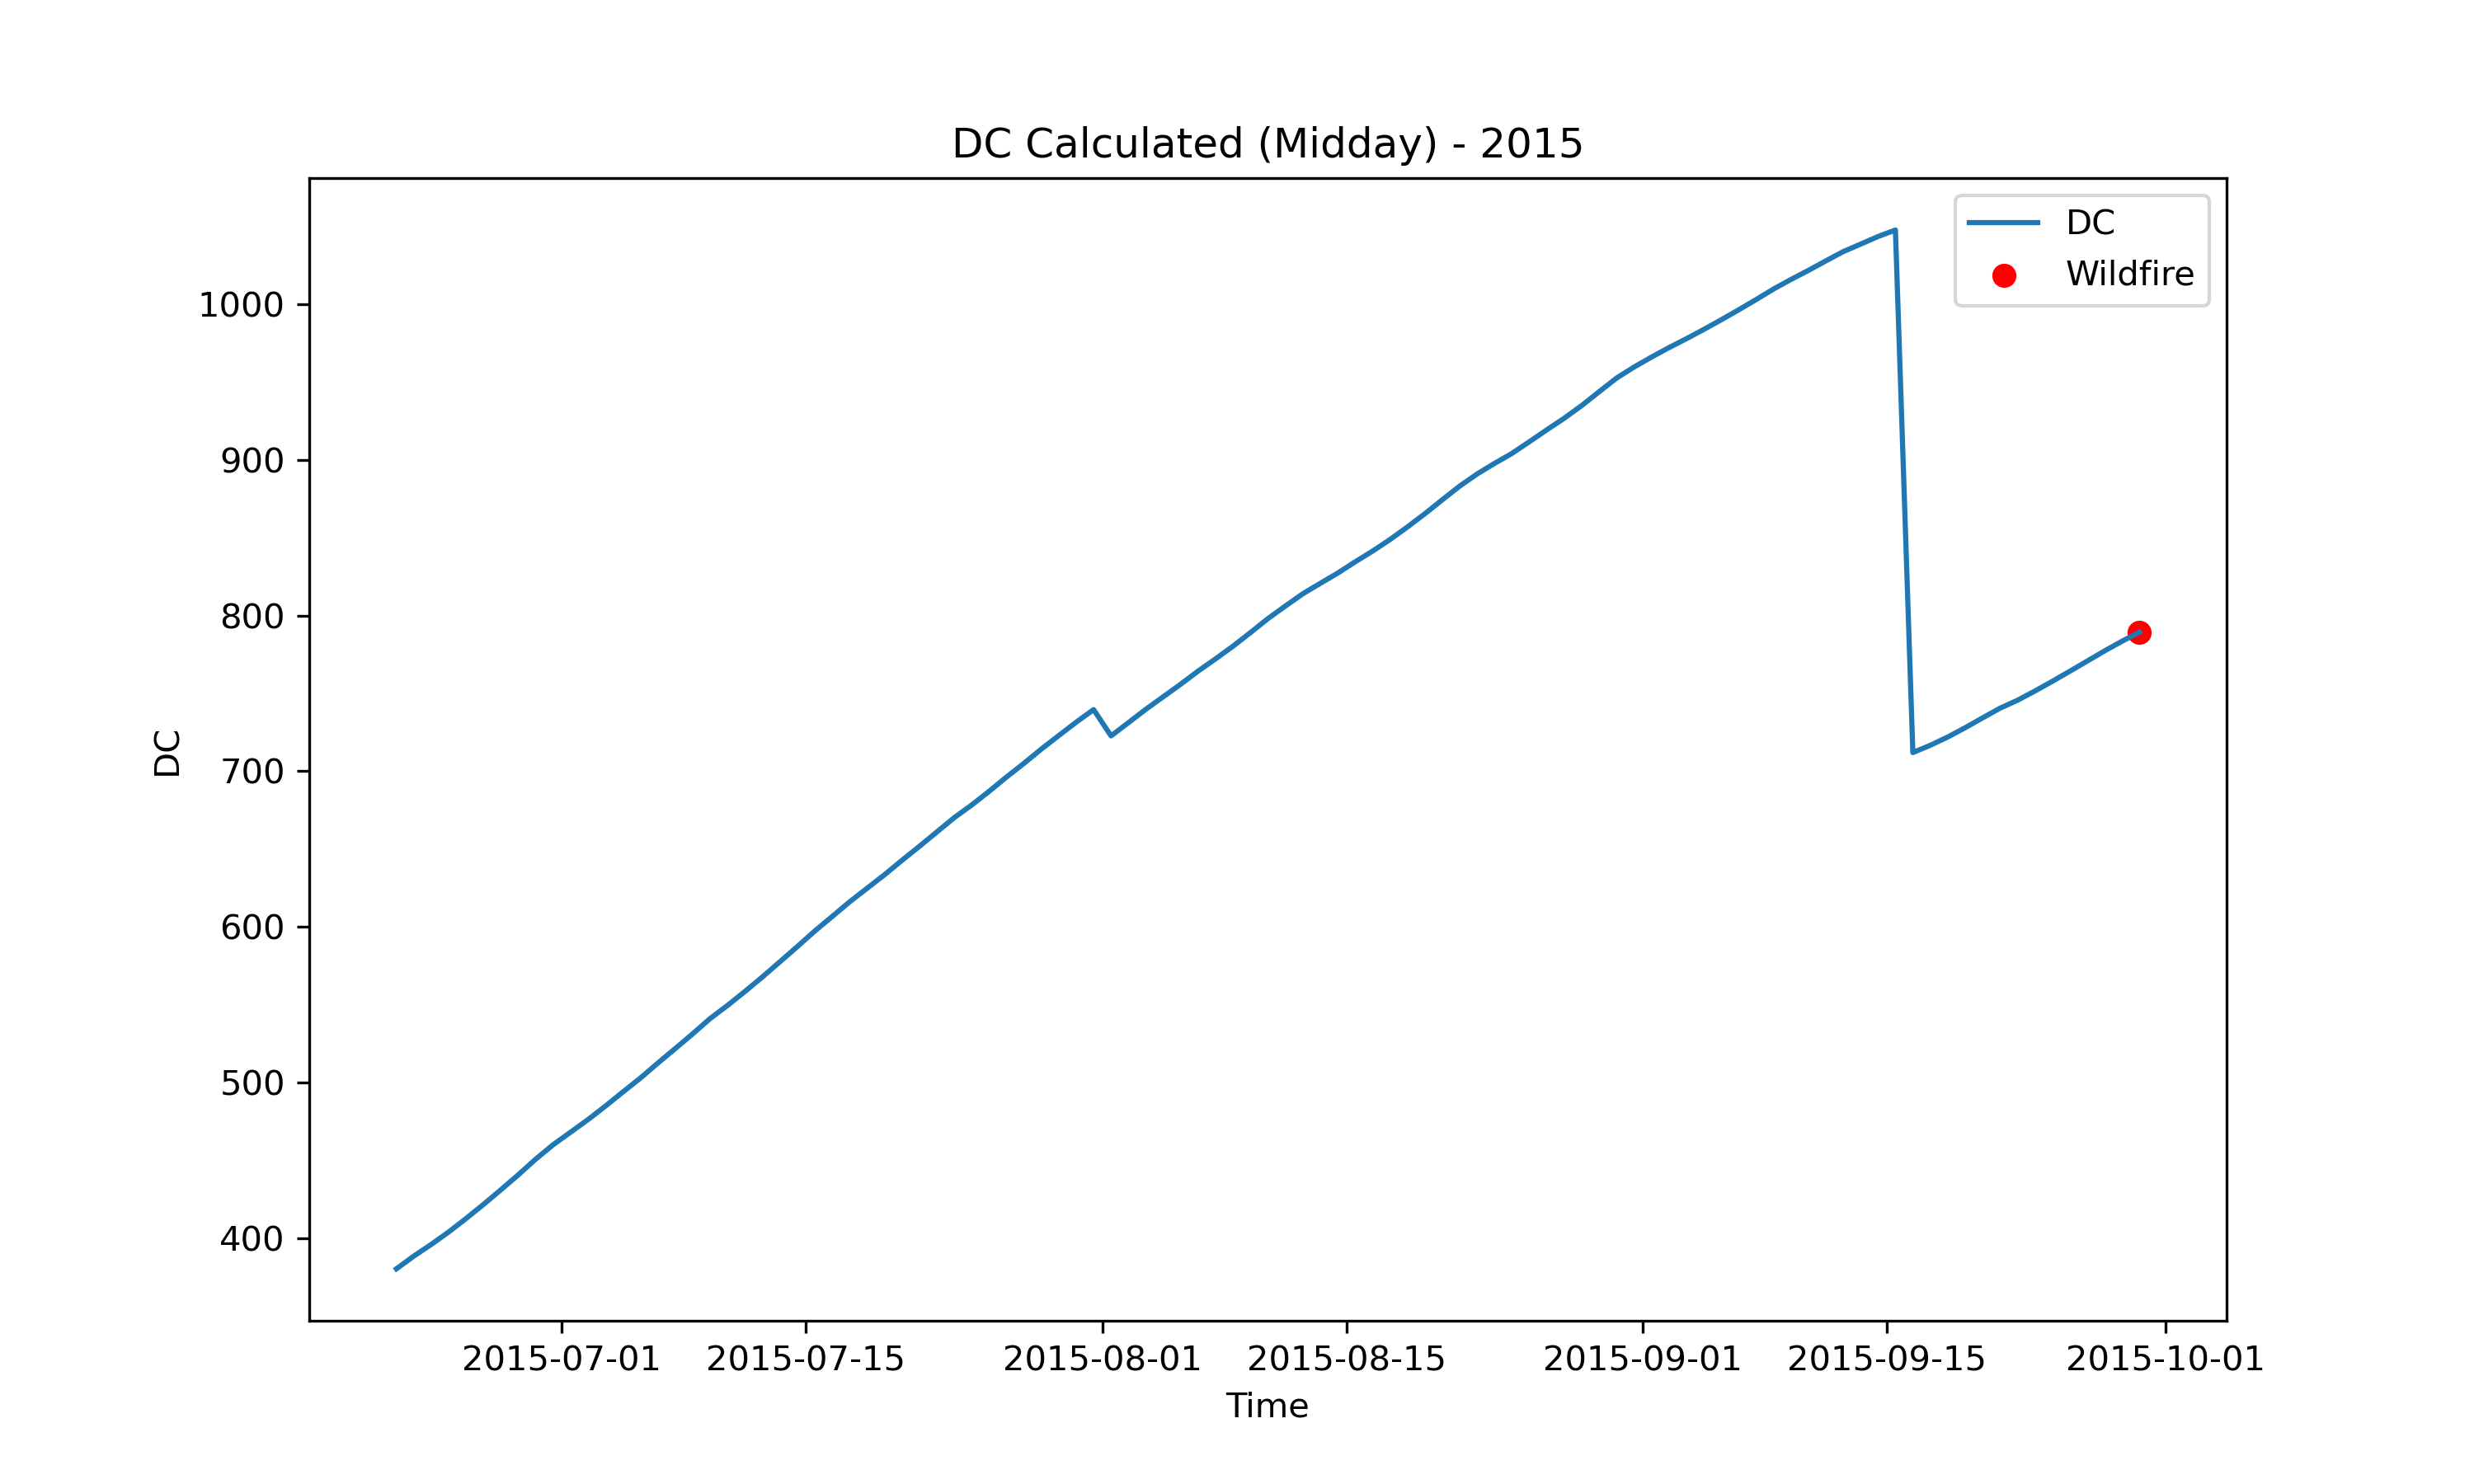
\includegraphics[width=\textwidth]{graphs/2015/2015CalcDC12.png}
        \caption{DC - Calculated value}
        \label{fig:dc_calculated_2015_midday}
    \end{subfigure}
    \label{fig:comparison_dc_midday_copernicus_calculated}
\end{figure}

\begin{figure}[h]
	\caption{Comparison of ISI calculated values and Copernicus at midday}
	\centering
	\begin{subfigure}{0.49\textwidth}
		\centering
		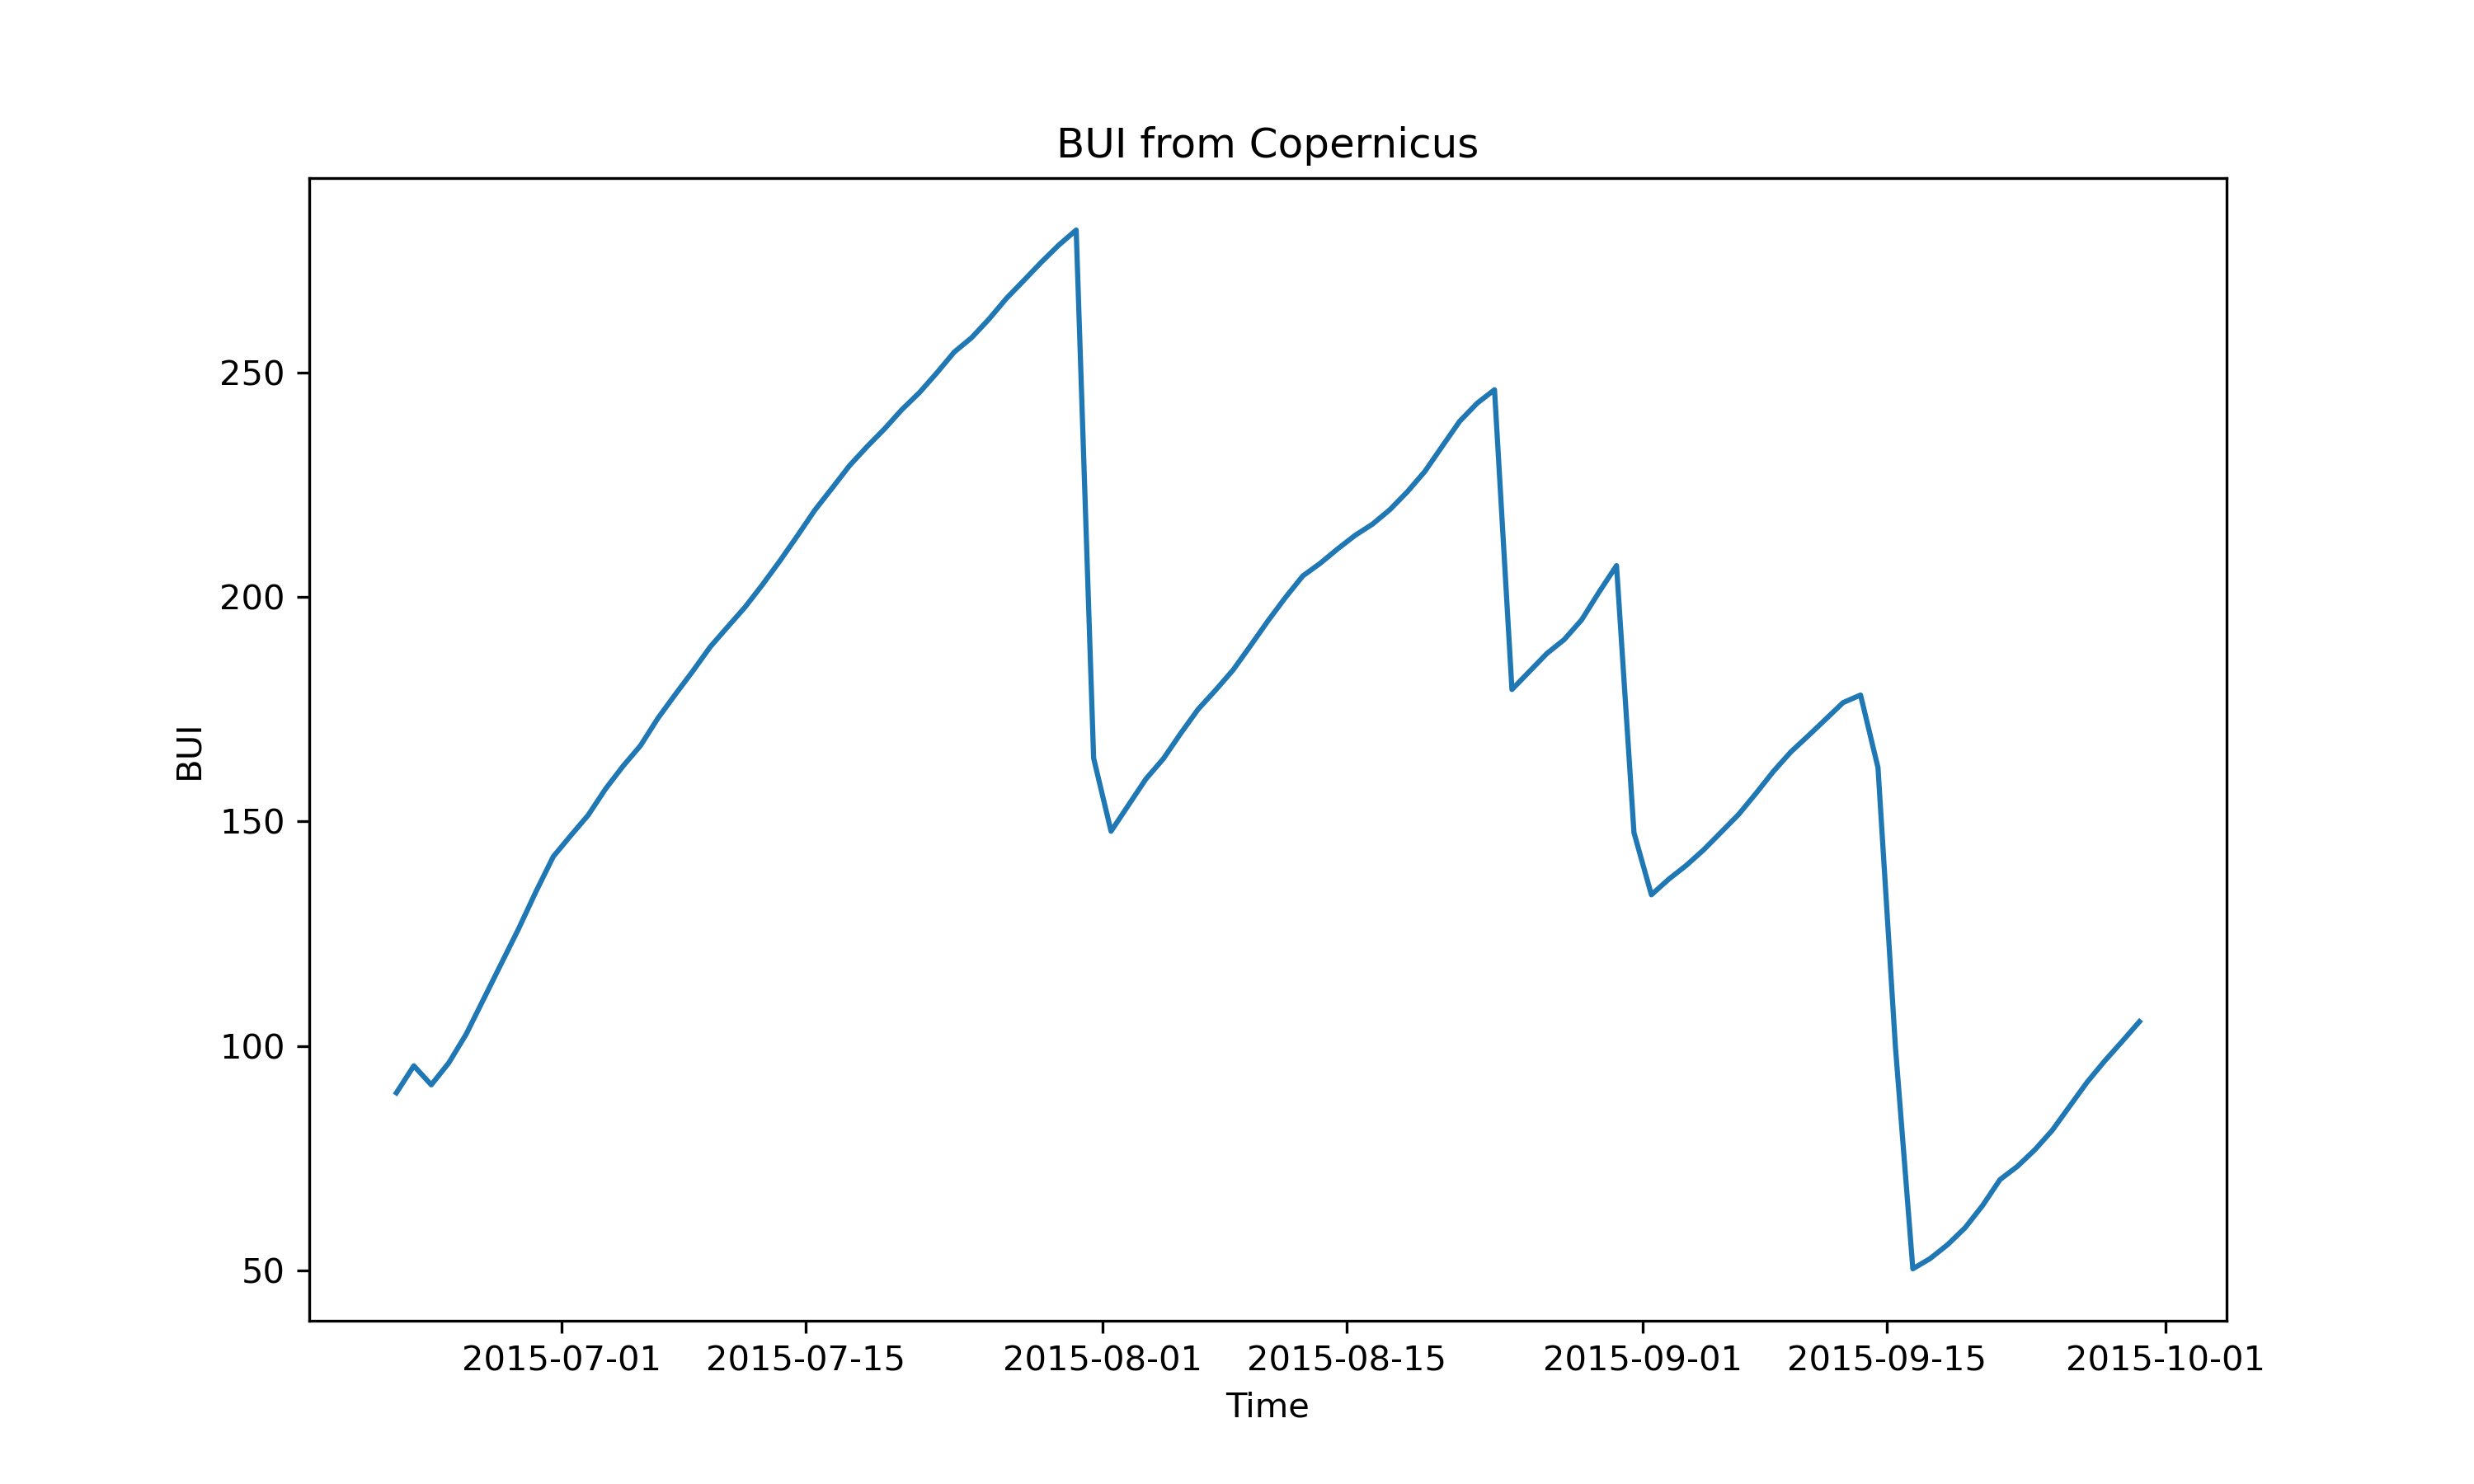
\includegraphics[width=\textwidth]{graphs/2015/2015CopernicusISI12.png}
		\caption{ISI - Copernicus}
		\label{fig:isi_copernicus_2015_midday}
	\end{subfigure}
	\hfill
	\begin{subfigure}{0.49\textwidth}
		\centering
		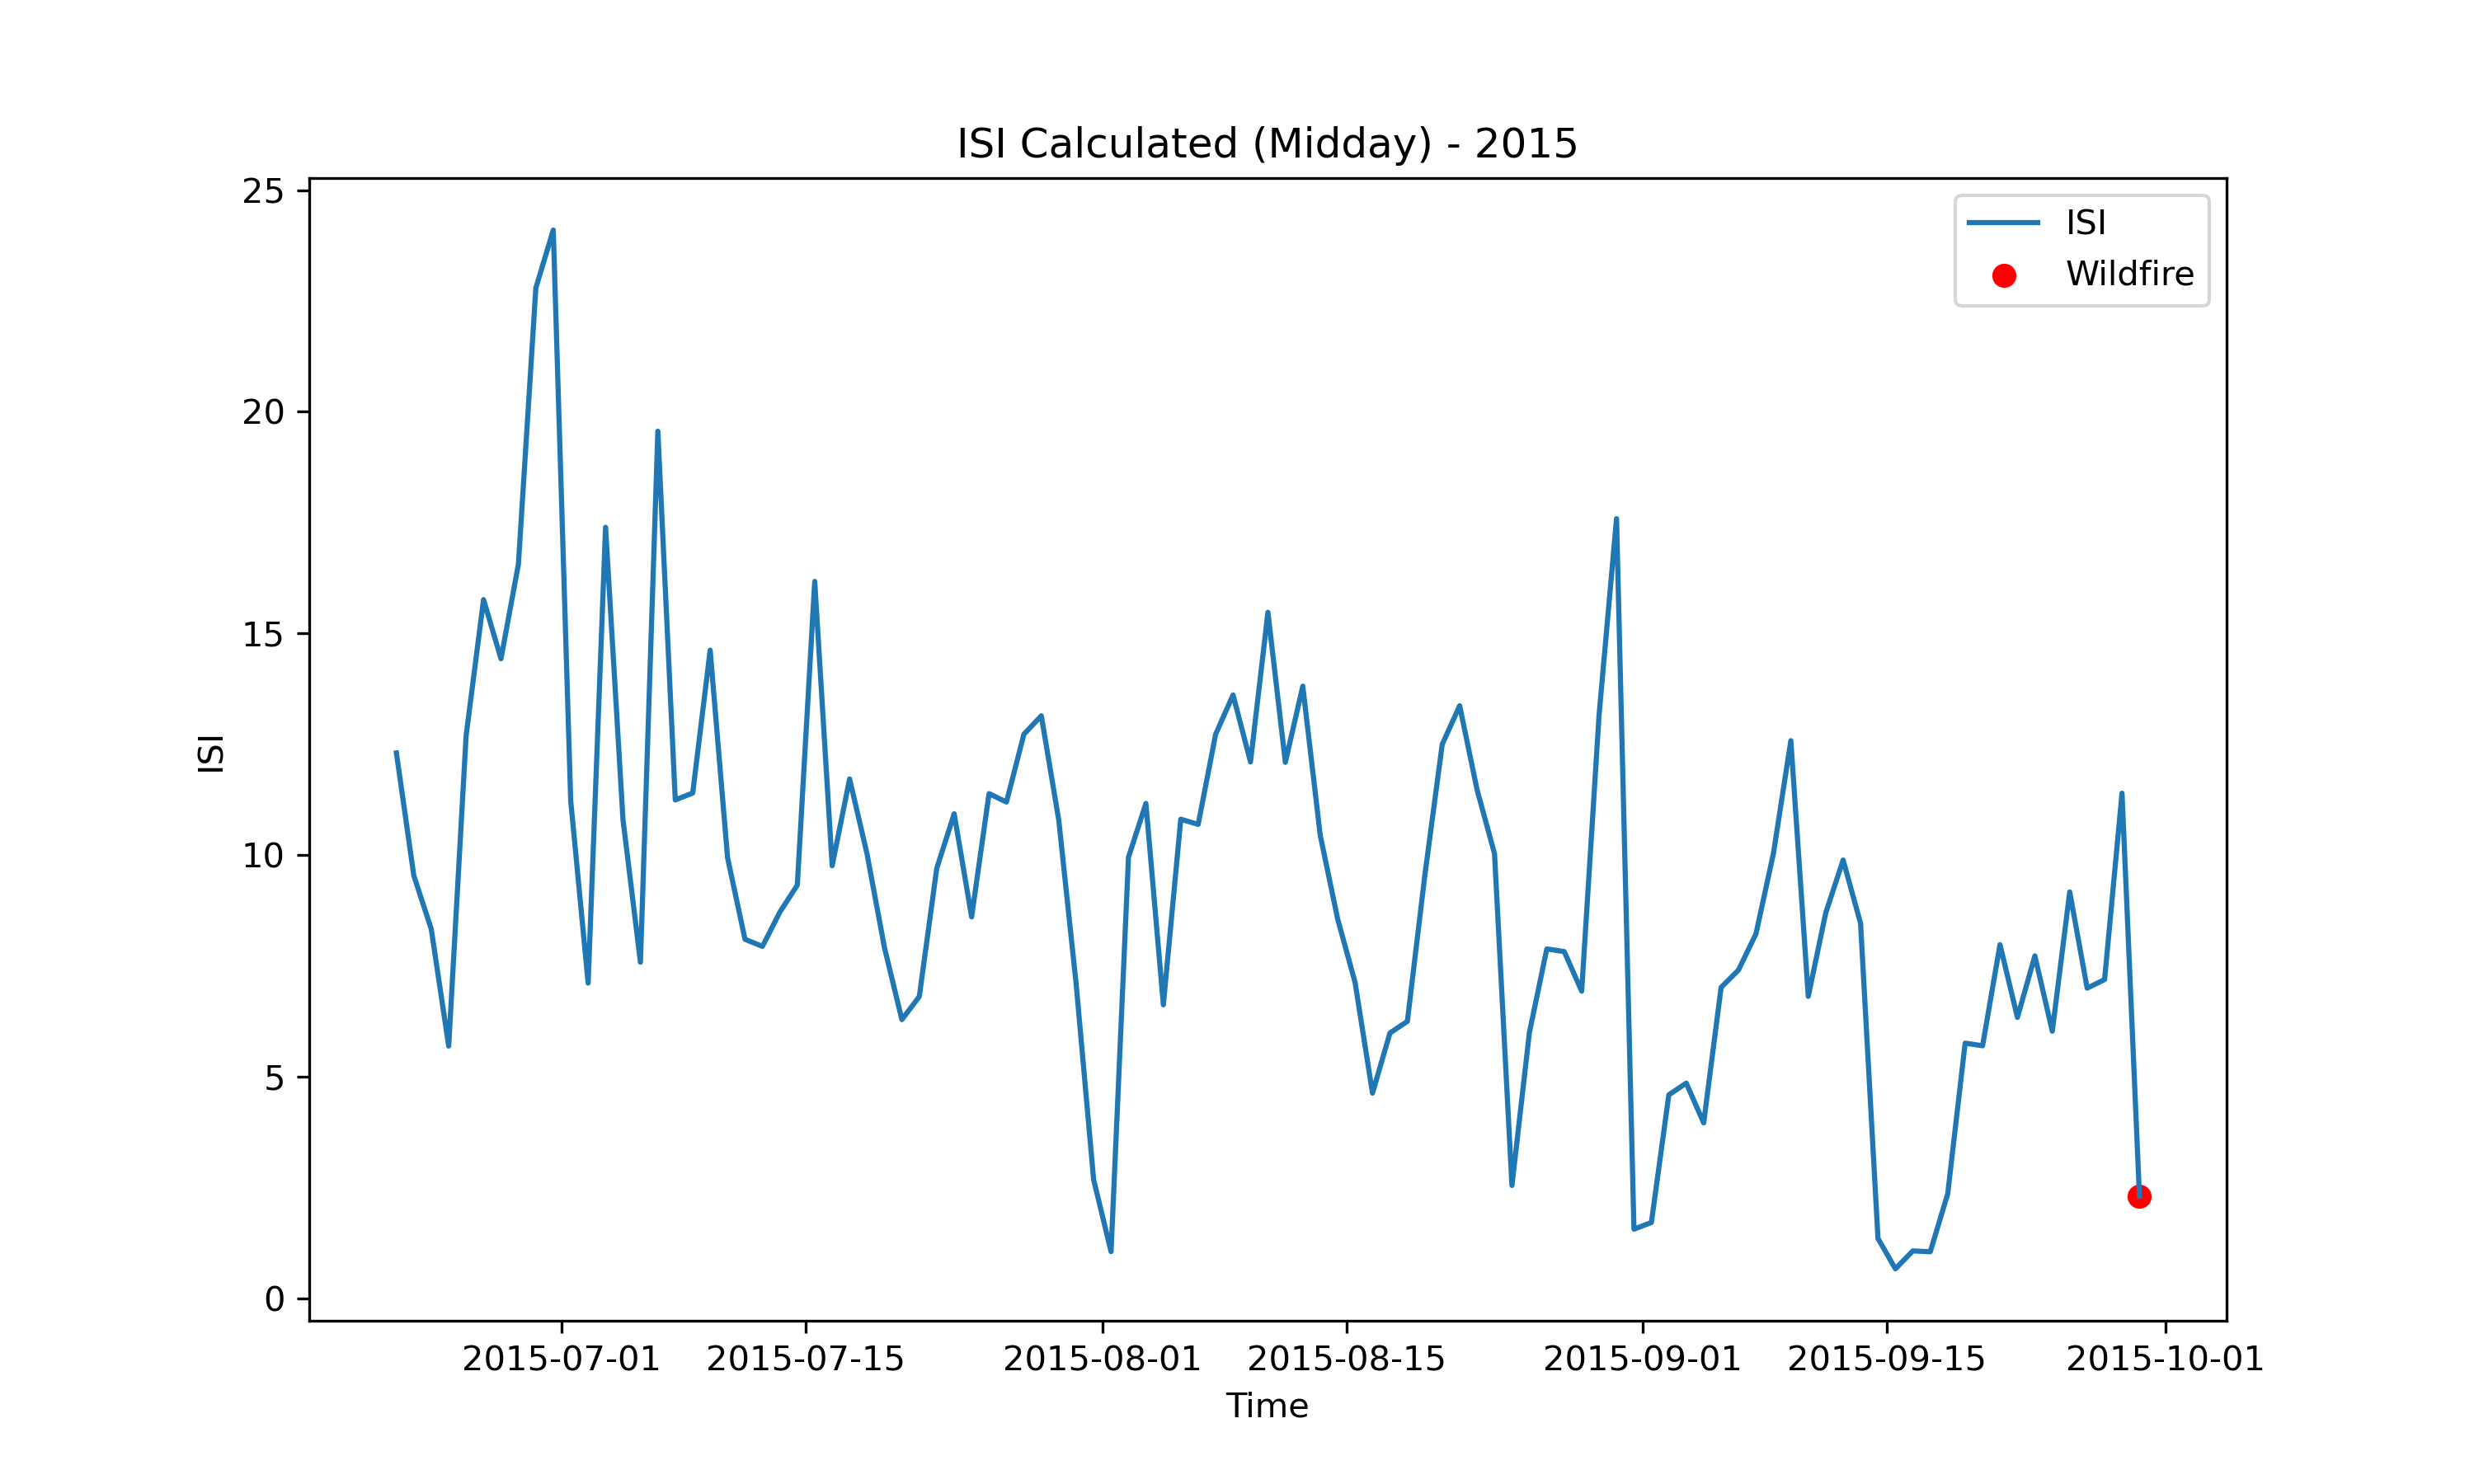
\includegraphics[width=\textwidth]{graphs/2015/2015CalcISI12.png}
		\caption{ISI - Calculated value}
		\label{fig:isi_calculated_2015_midday}
	\end{subfigure}
	\label{fig:comparison_isi_midday_copernicus_calculated}
\end{figure}

\begin{figure}[h]
	\caption{Comparison of BUI calculated values and Copernicus at midday}
	\centering
	\begin{subfigure}{0.49\textwidth}
		\centering
		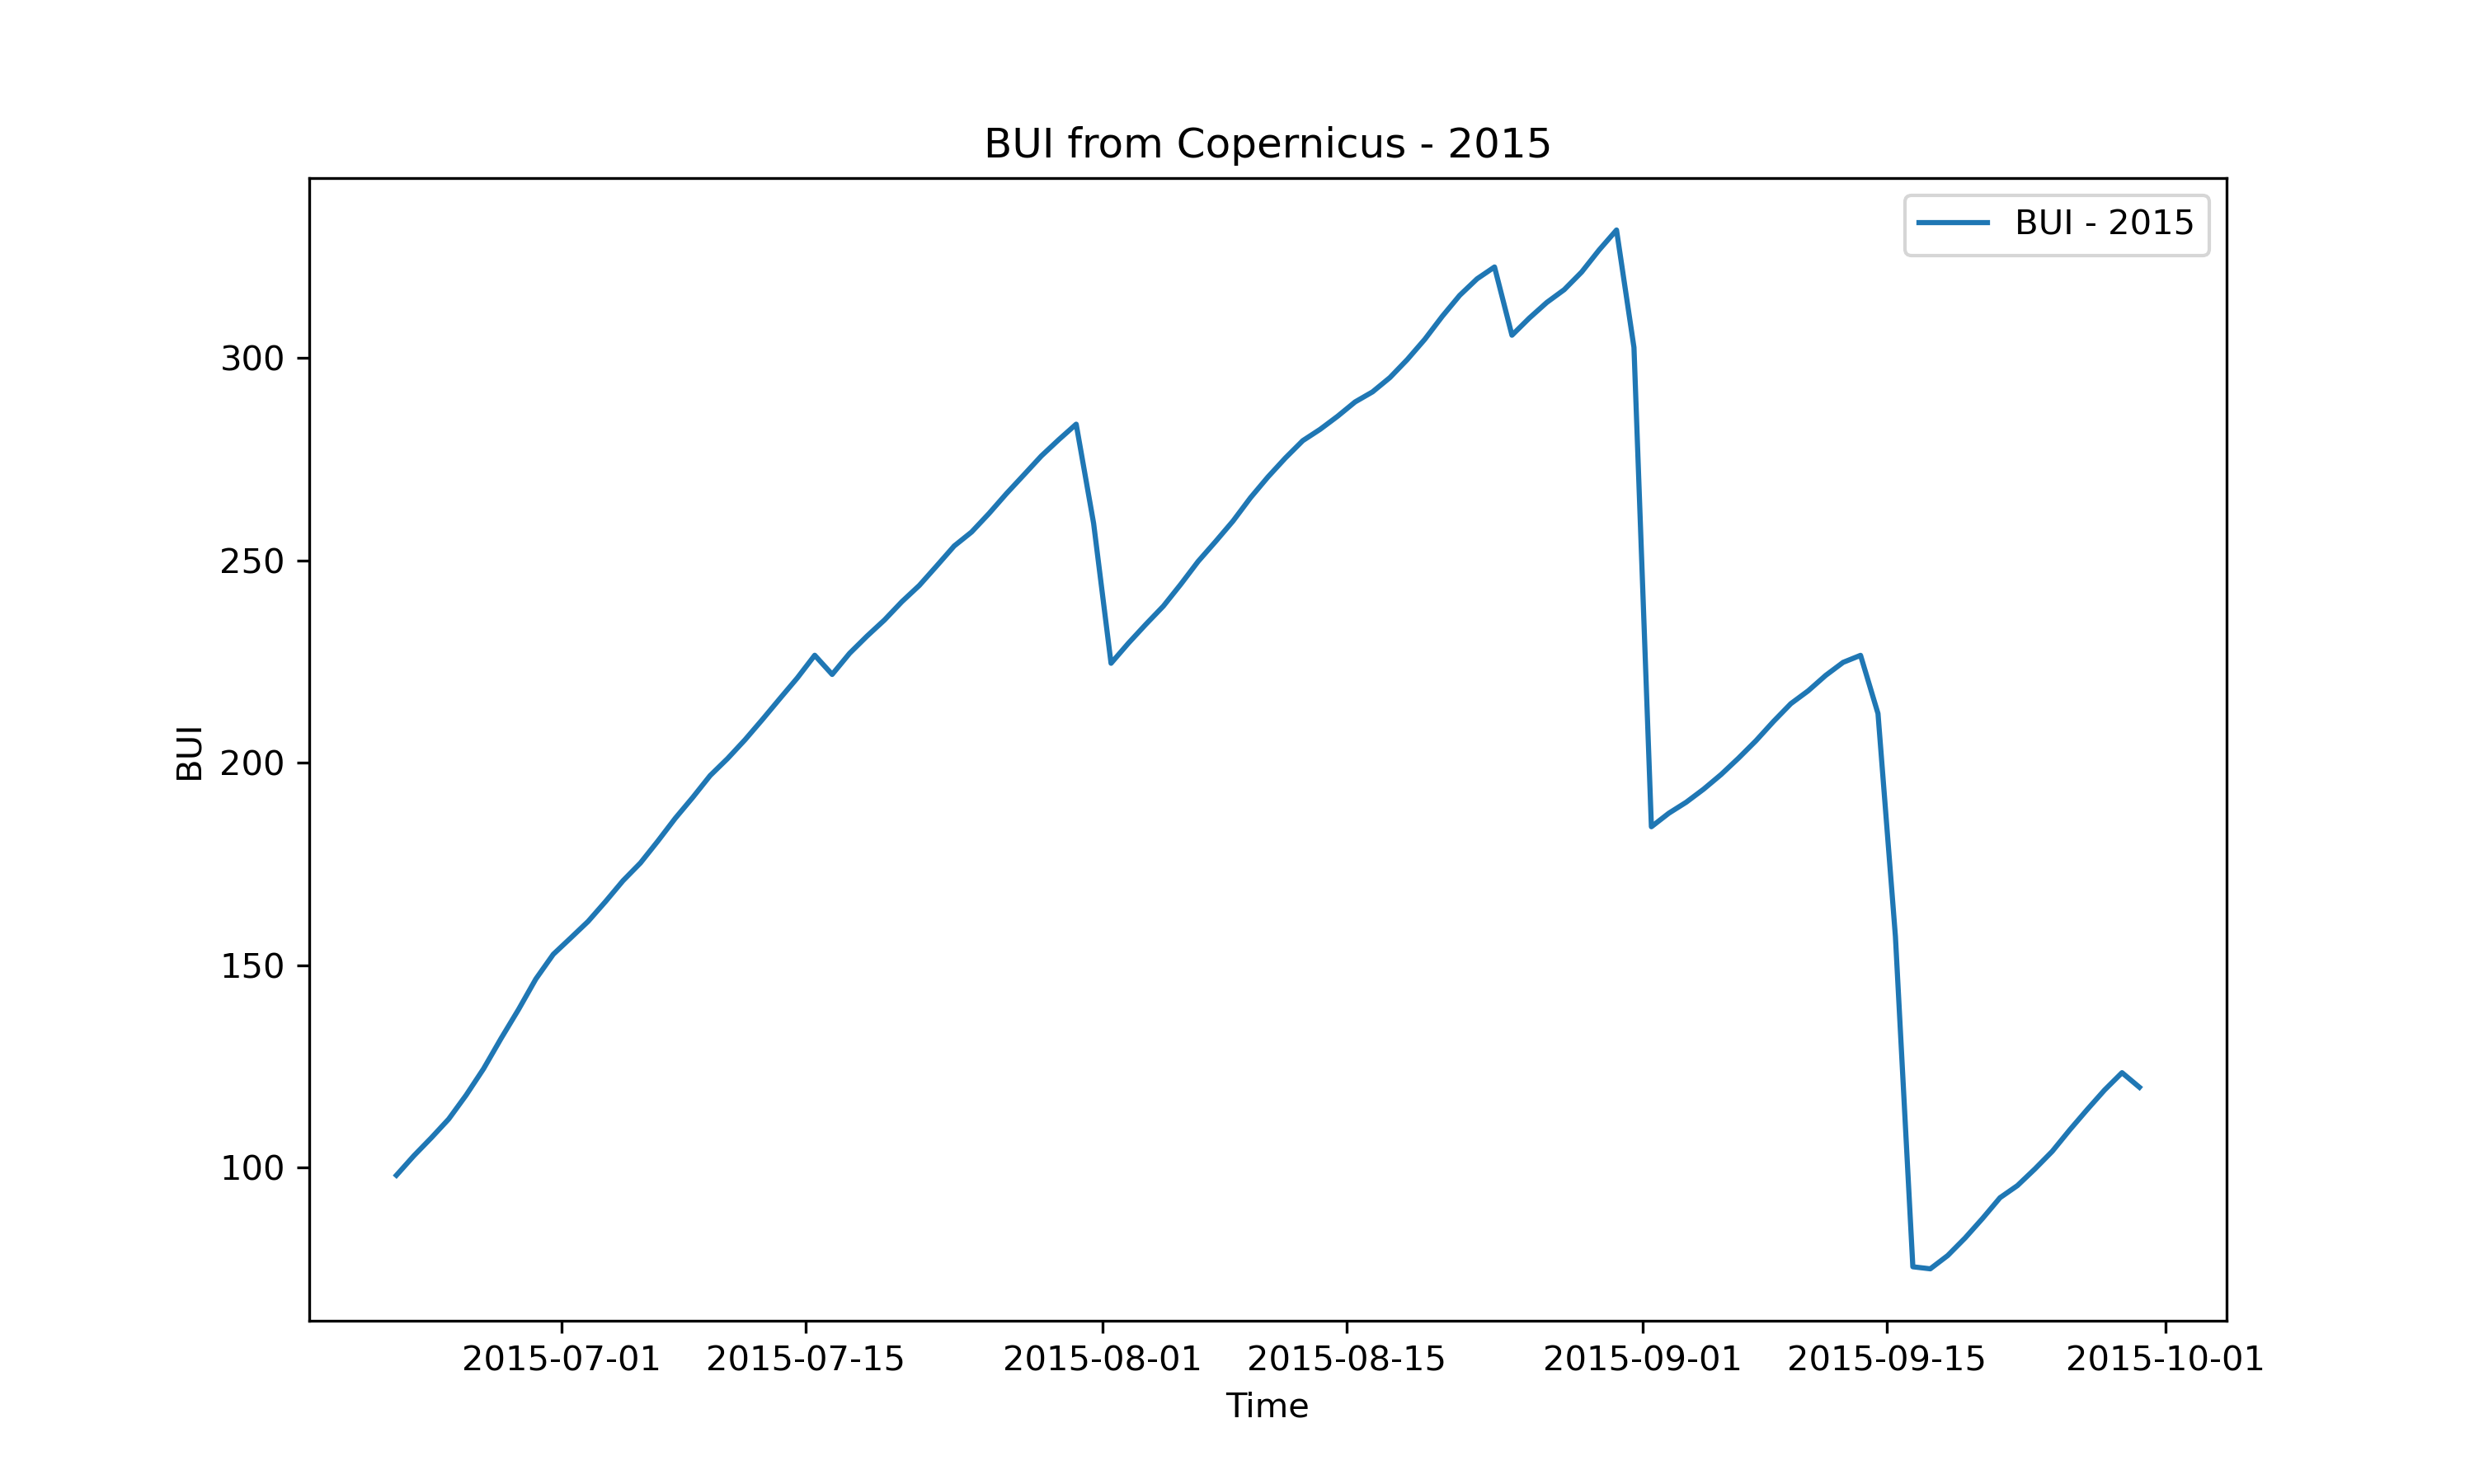
\includegraphics[width=\textwidth]{graphs/2015/2015CopernicusBUI12.png}
		\caption{BUI - Copernicus}
		\label{fig:bui_copernicus_2015_midday}
	\end{subfigure}
	\hfill
	\begin{subfigure}{0.49\textwidth}
		\centering
		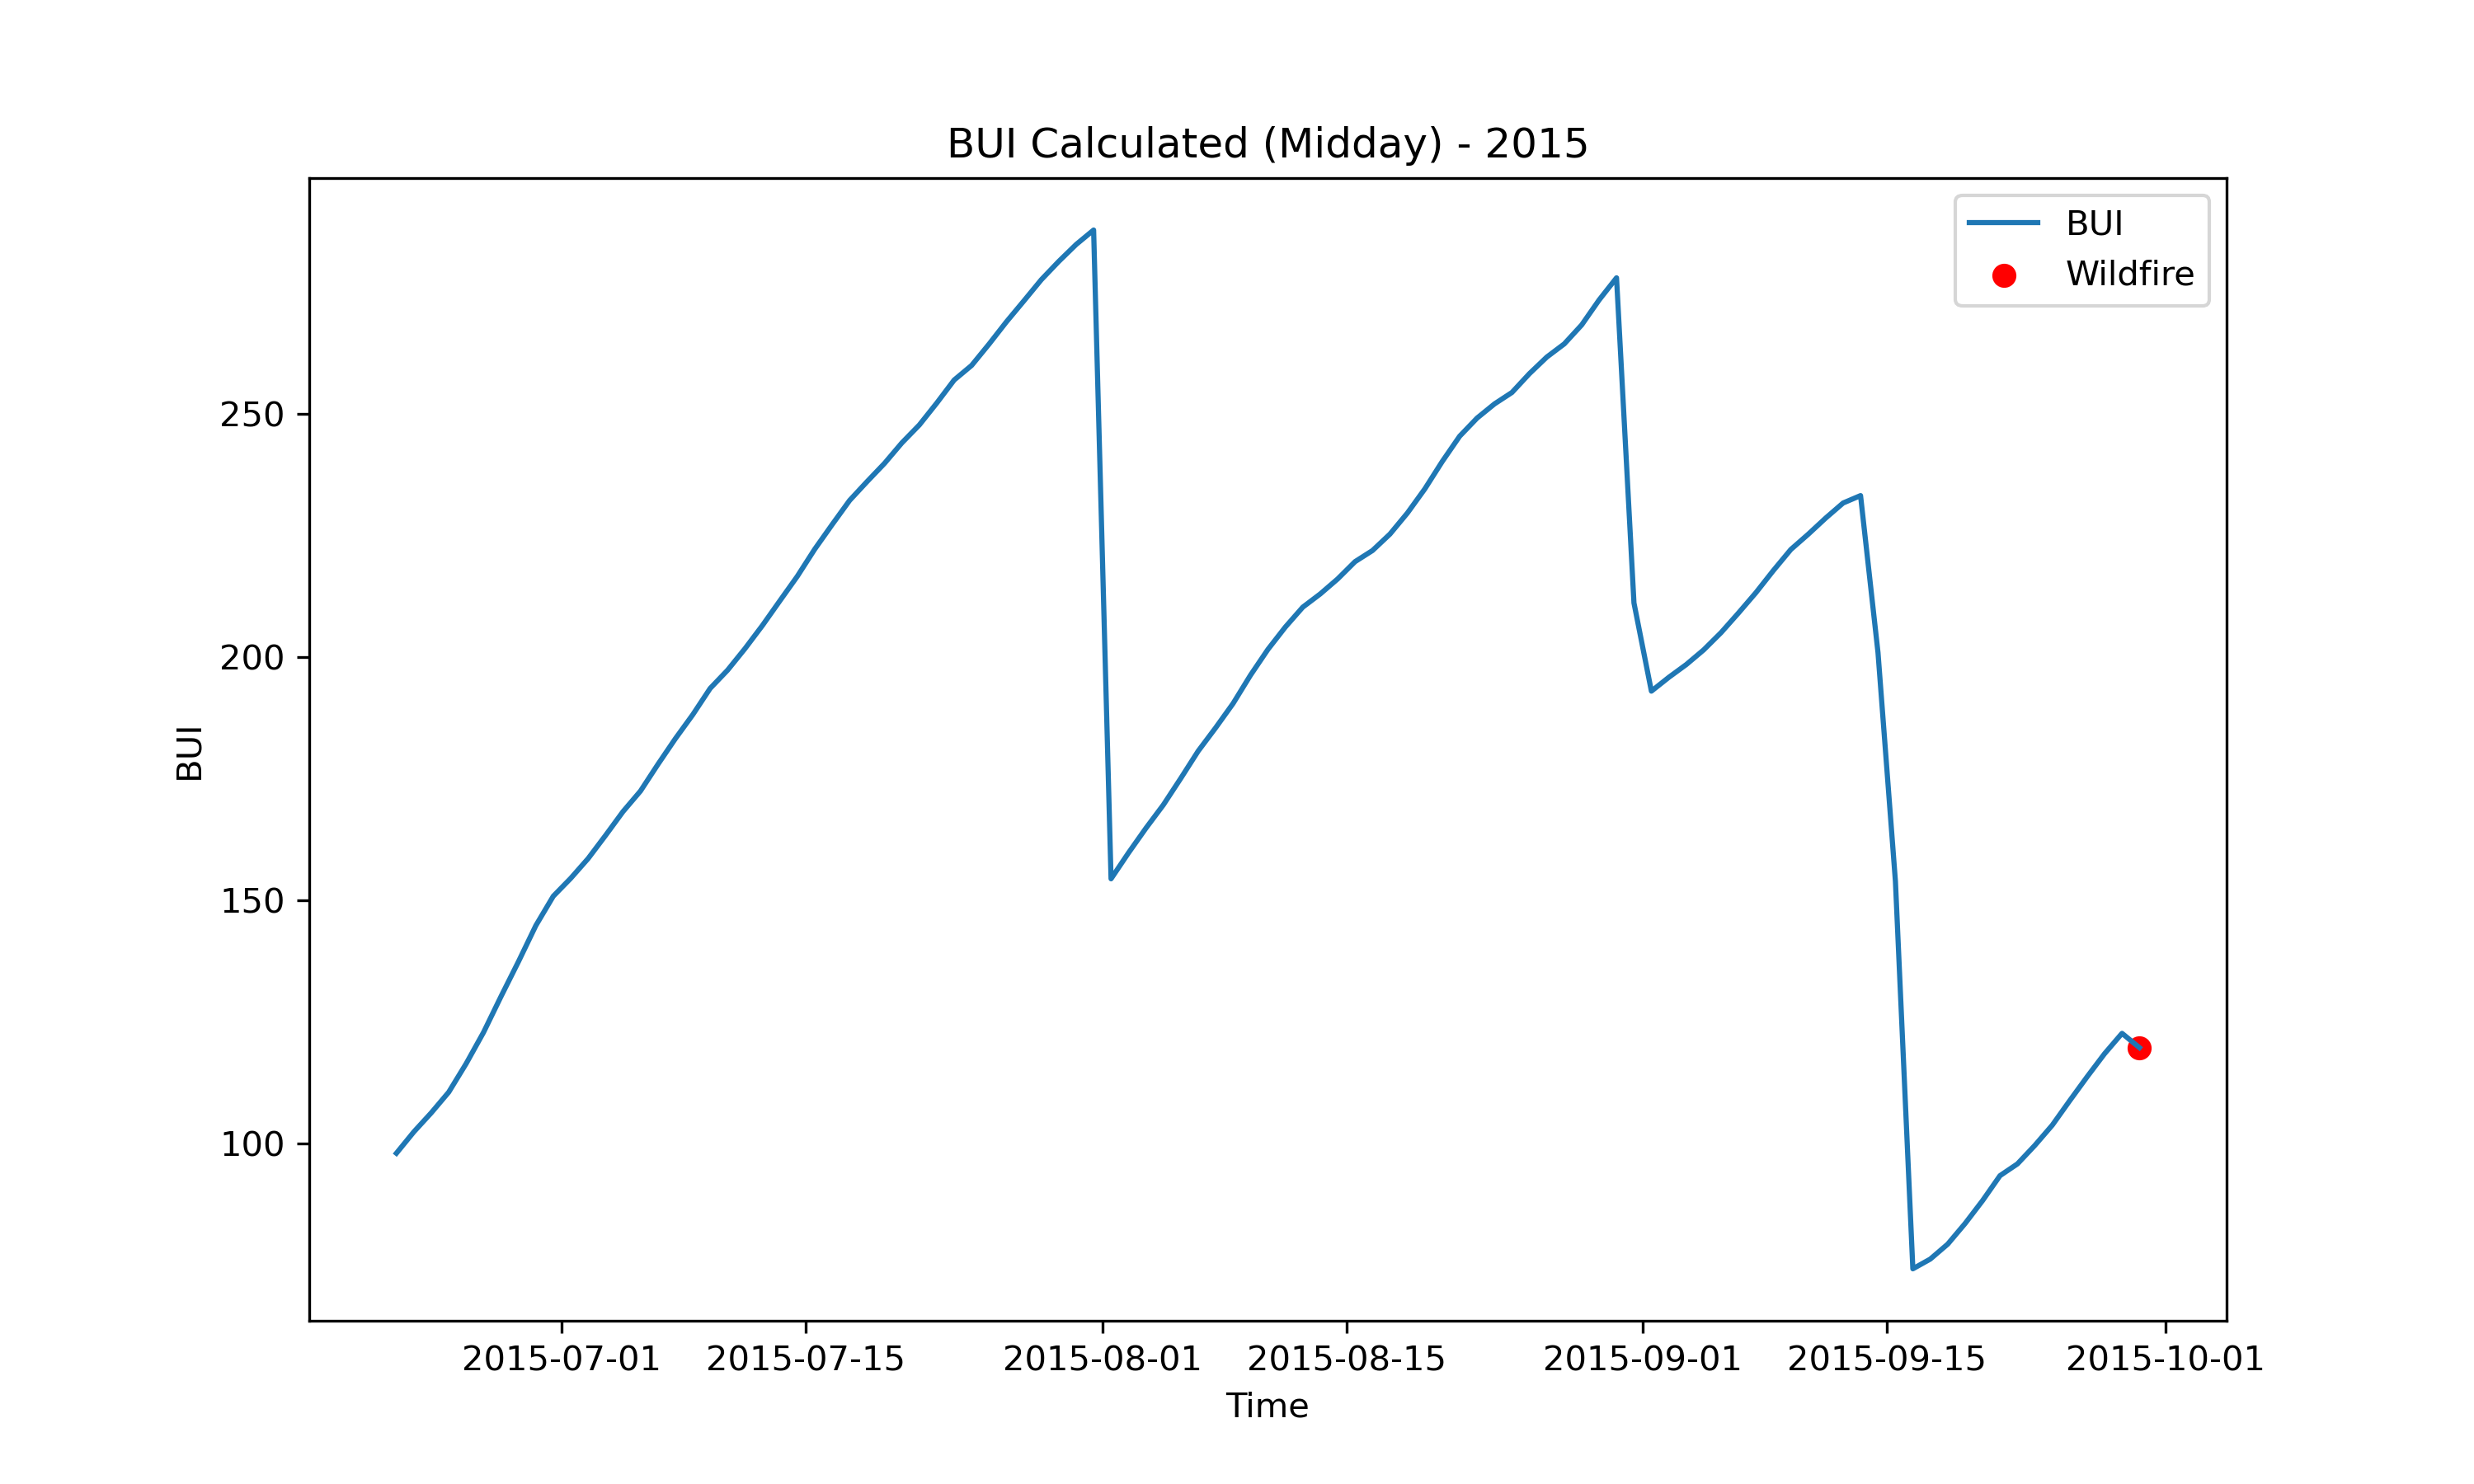
\includegraphics[width=\textwidth]{graphs/2015/2015CalcBUI12.png}
		\caption{BUI - Calculated value}
		\label{fig:bui_calculated_2015_midday}
	\end{subfigure}
	\label{fig:comparison_bui_midday_copernicus_calculated}
\end{figure}

\FloatBarrier

\subsection{Fogo de 2019}


\begin{figure}[h]
	\caption{Comparison of FWI calculated values and Copernicus at midday - 2019}
	\centering
	\begin{subfigure}{0.49\textwidth}
		\centering
		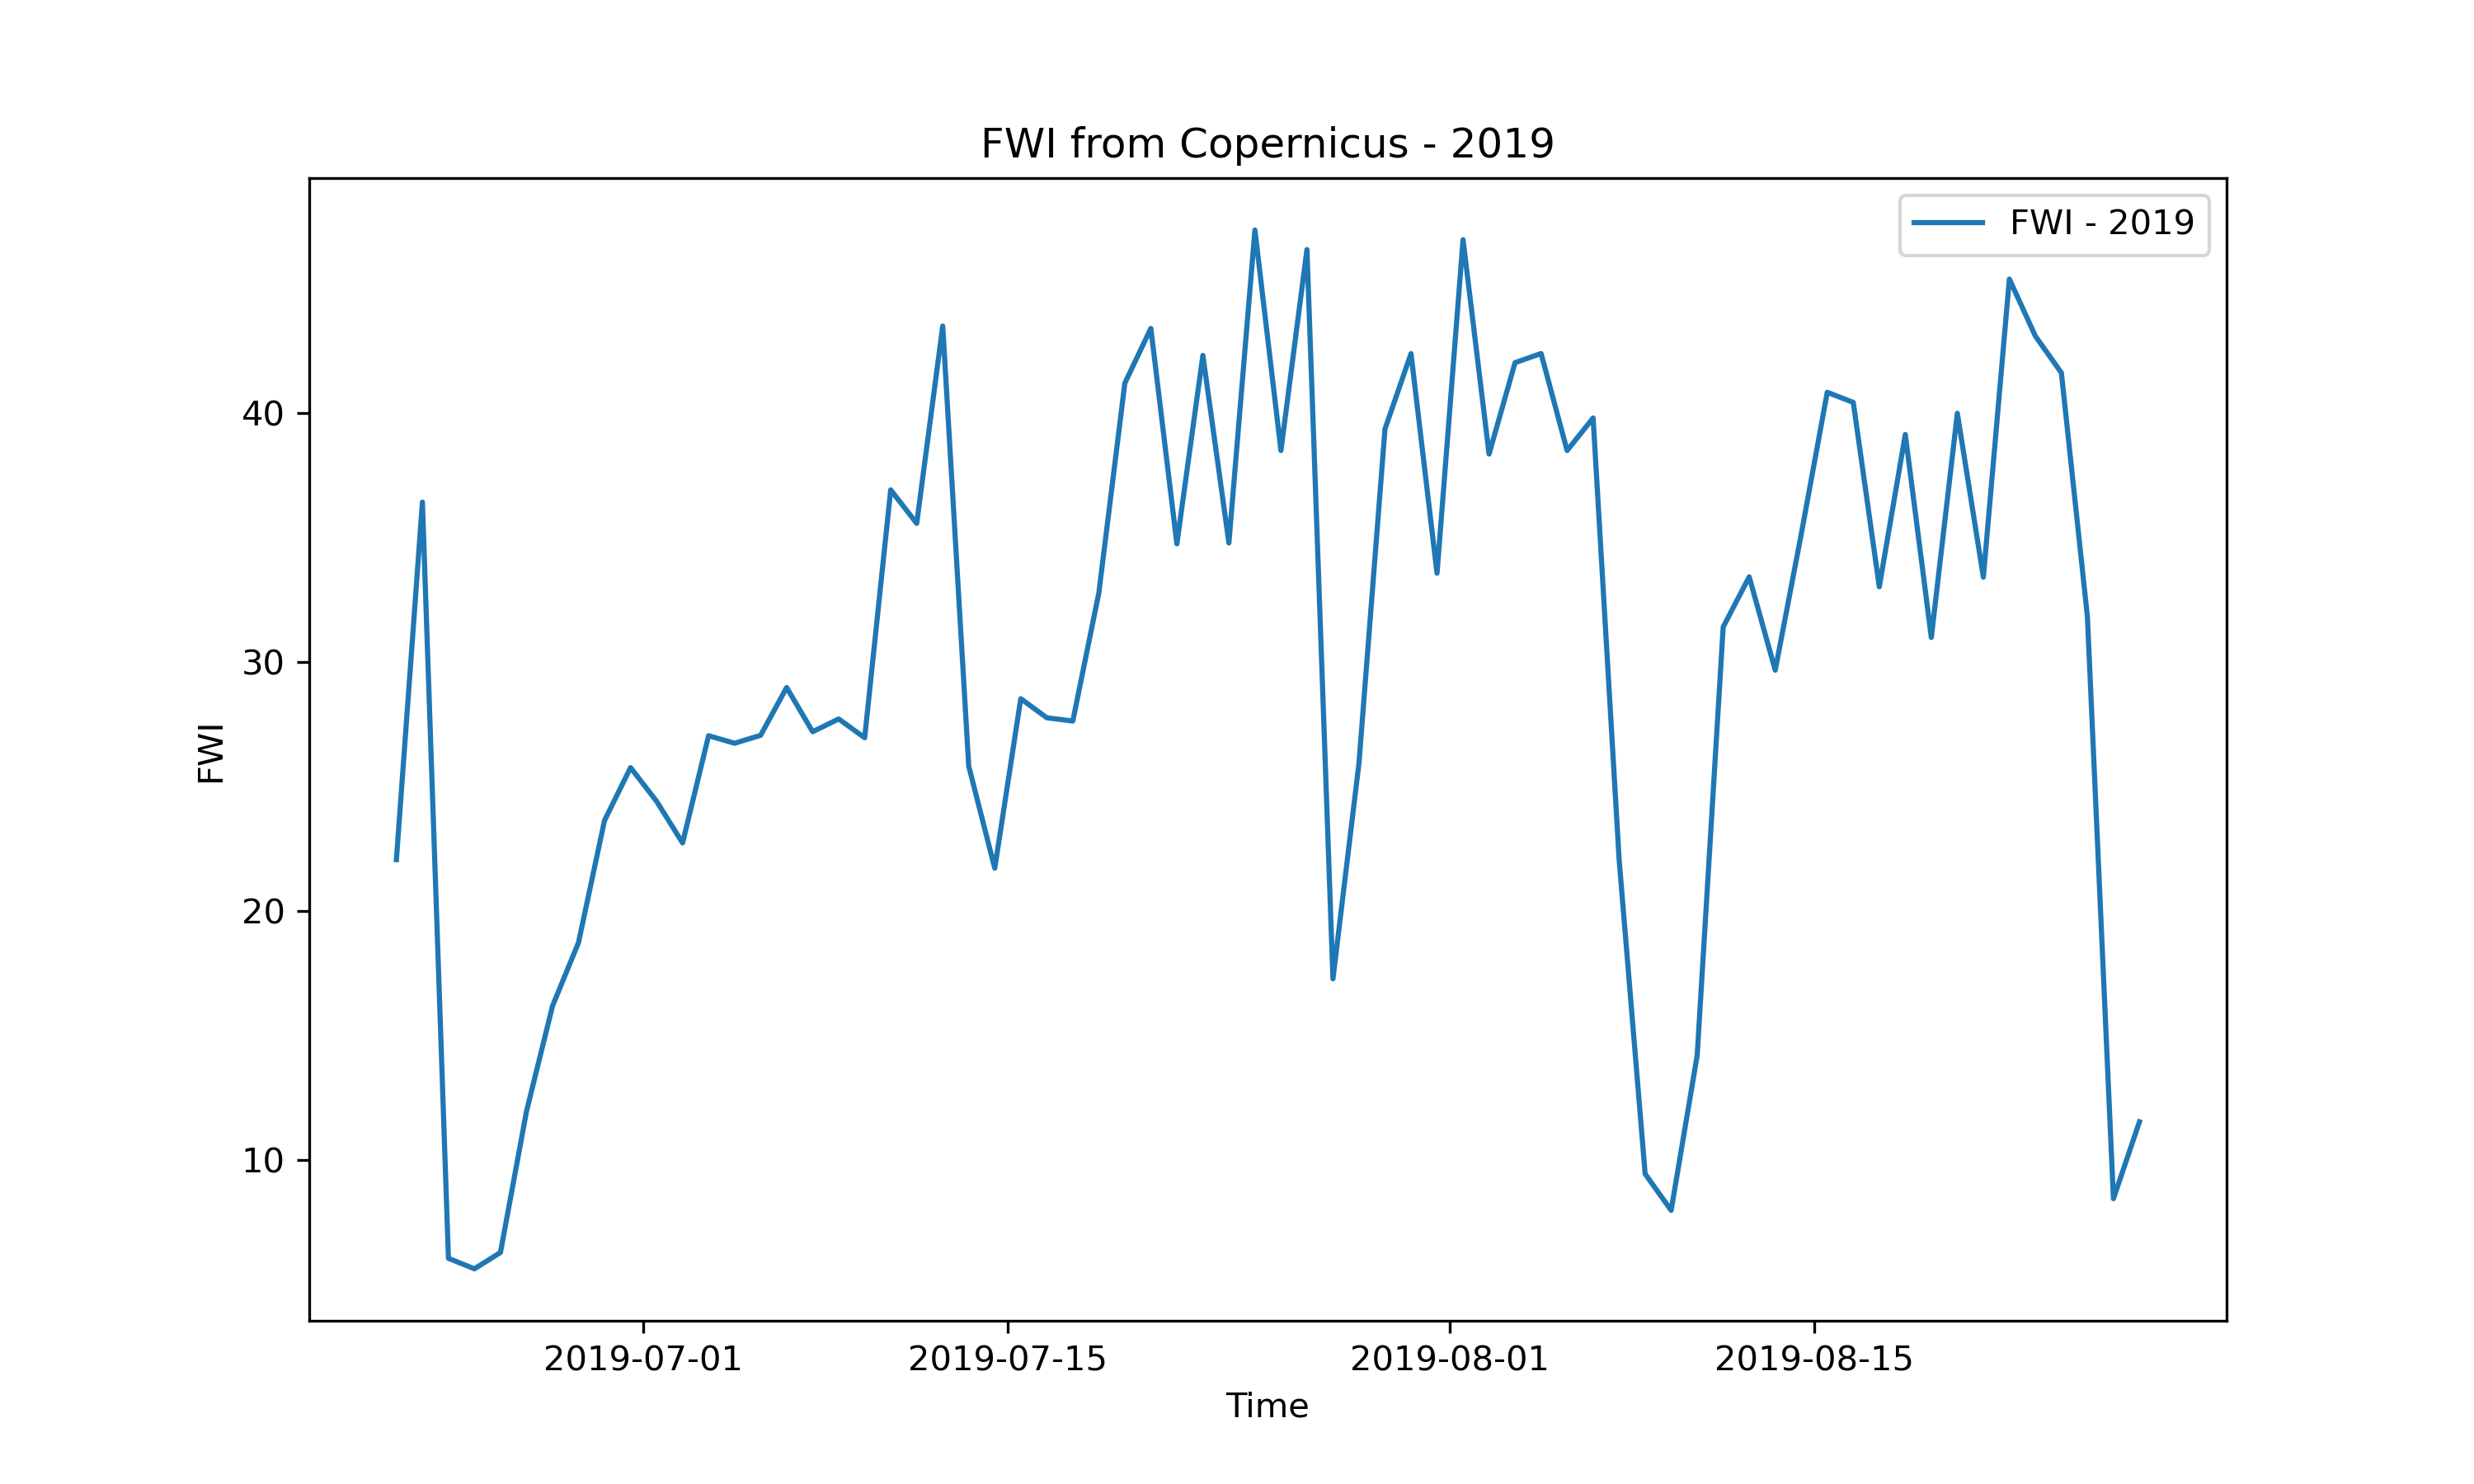
\includegraphics[width=\textwidth]{graphs/2019/2019CopernicusFWI12.png}
		\caption{FWI - Copernicus}
		\label{fig:fwi_copernicus_2019_midday}
	\end{subfigure}
	\hfill
	\begin{subfigure}{0.49\textwidth}
		\centering
		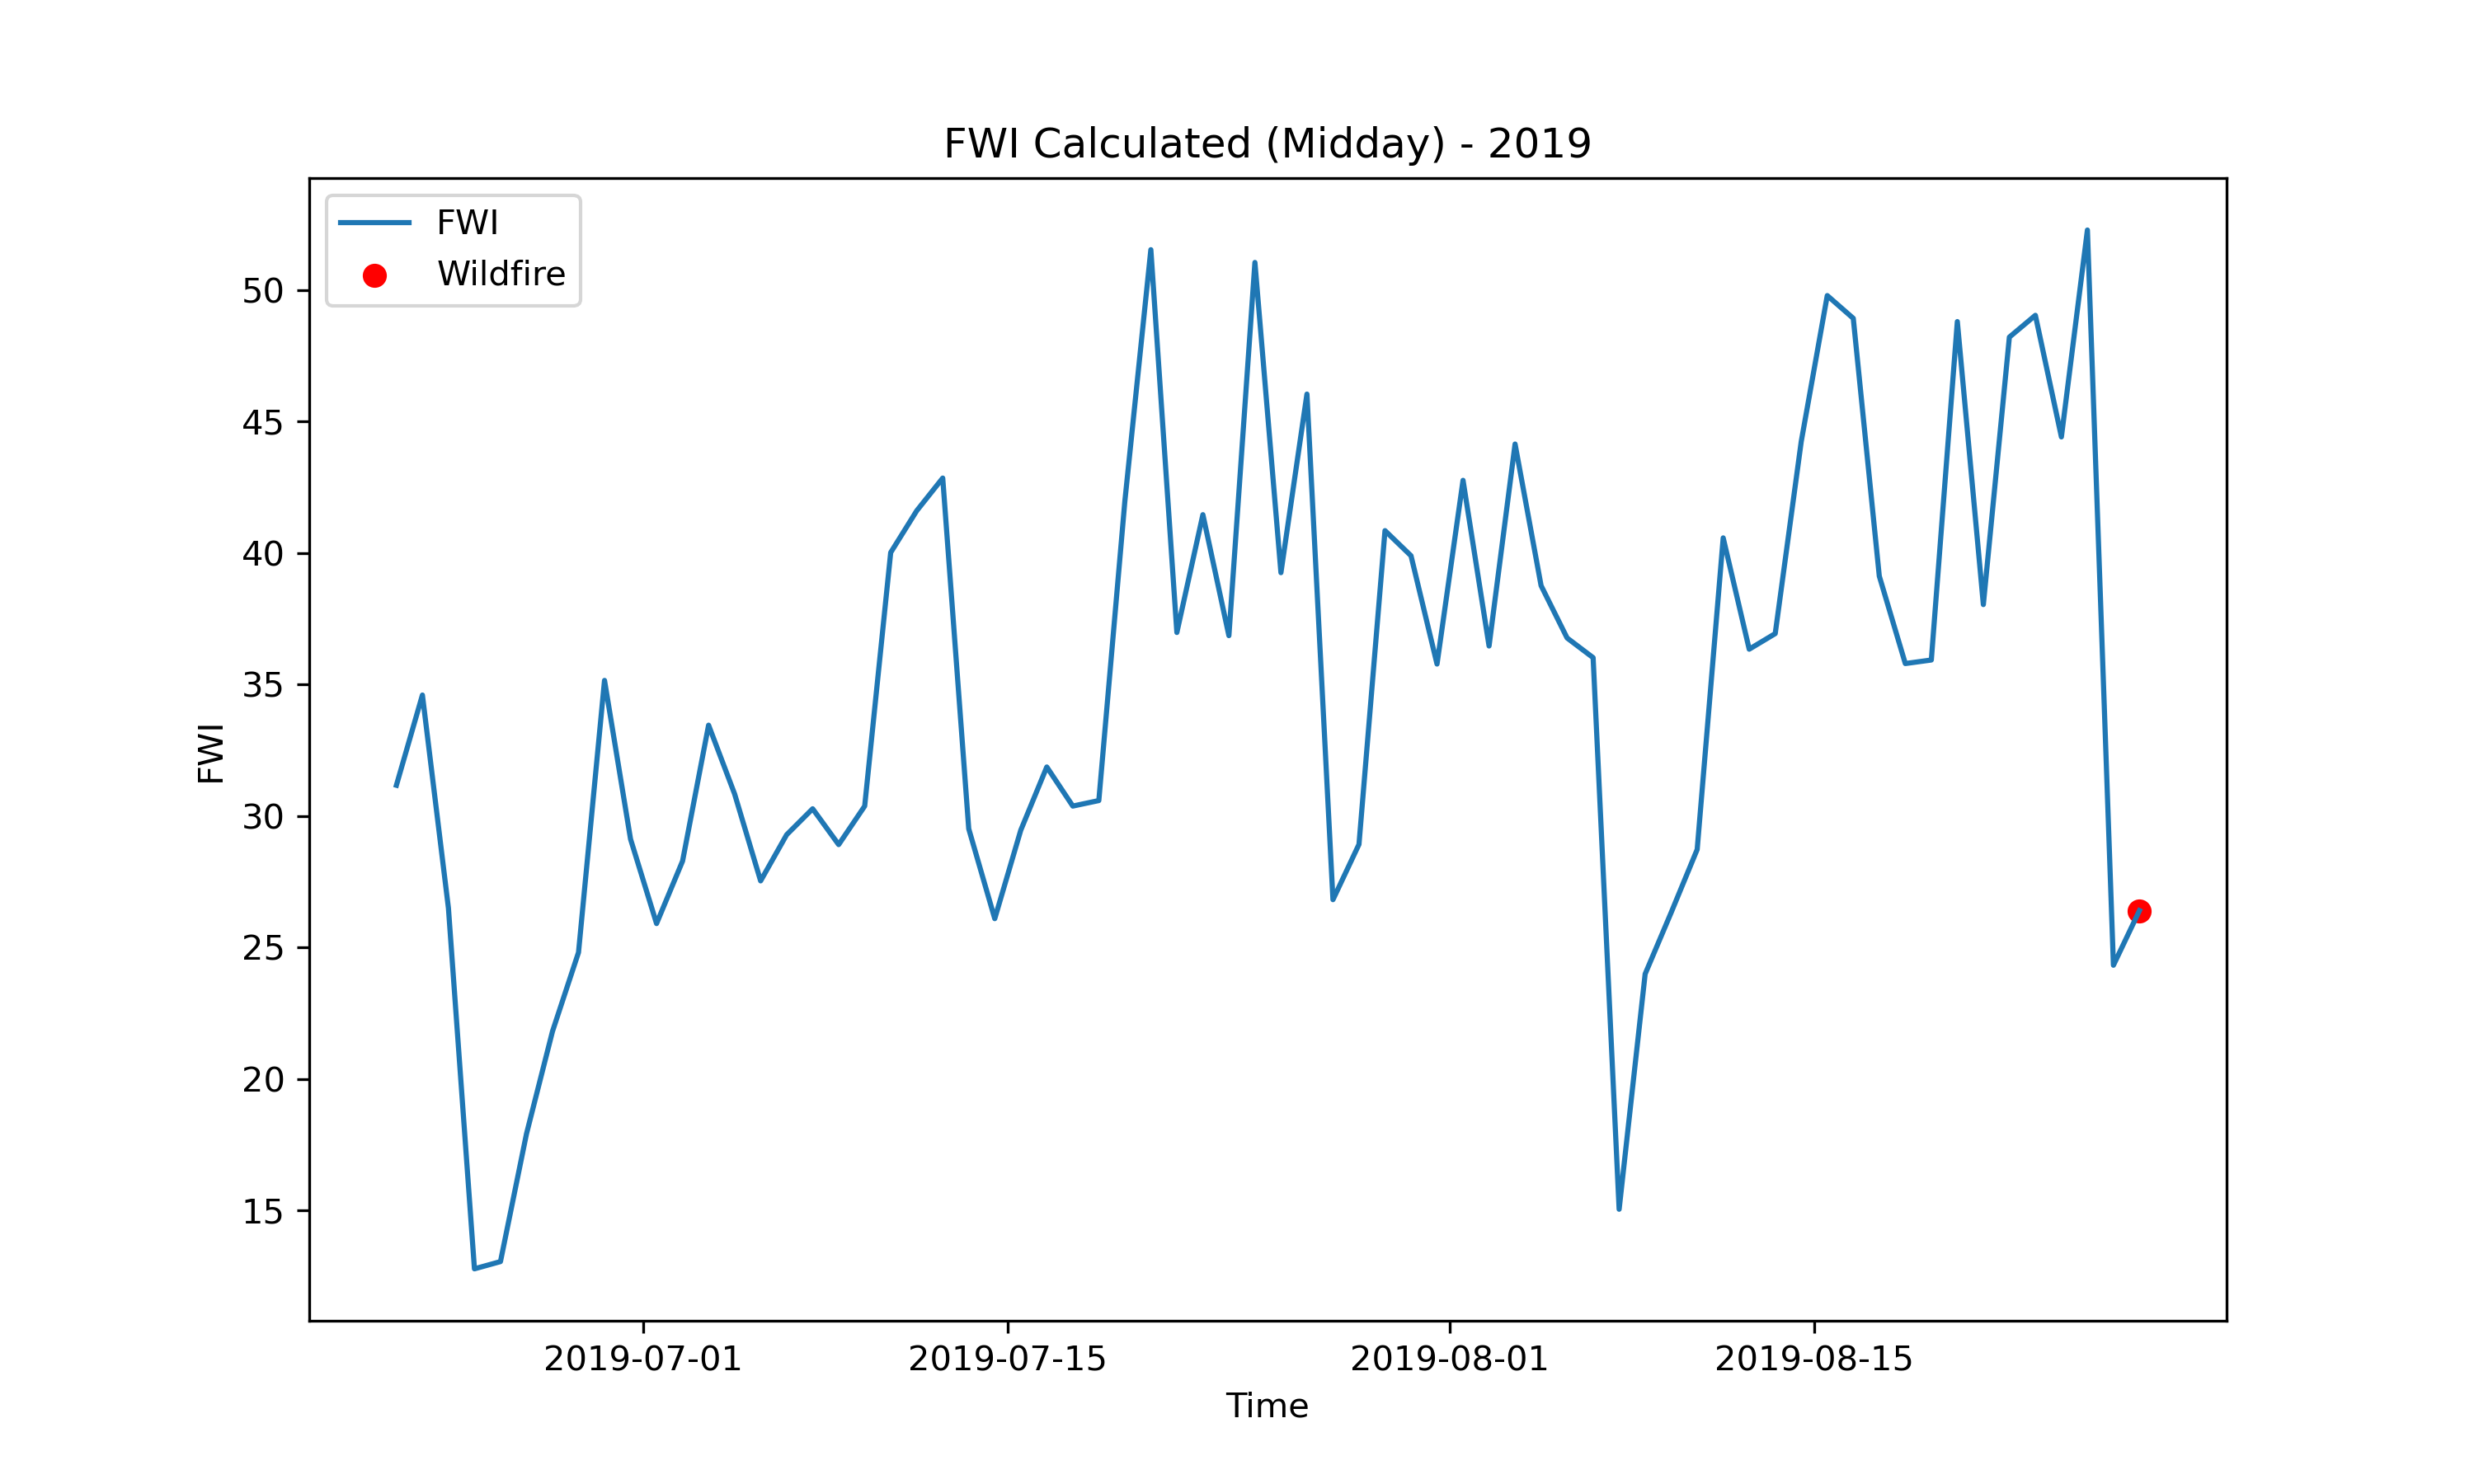
\includegraphics[width=\textwidth]{graphs/2019/2019CalcFWI12.png}
		\caption{FWI - Calculated value}
		\label{fig:fwi_calculated_2019_midday}
	\end{subfigure}
	\label{fig:comparison_fwi_2019_midday_copernicus_calculated}
\end{figure}


\FloatBarrier

\subsection{Fogo de 2022}

\begin{figure}[h]
	\caption{Comparison of FWI calculated values and Copernicus at midday - 2022}
	\centering
	\begin{subfigure}{0.49\textwidth}
		\centering
		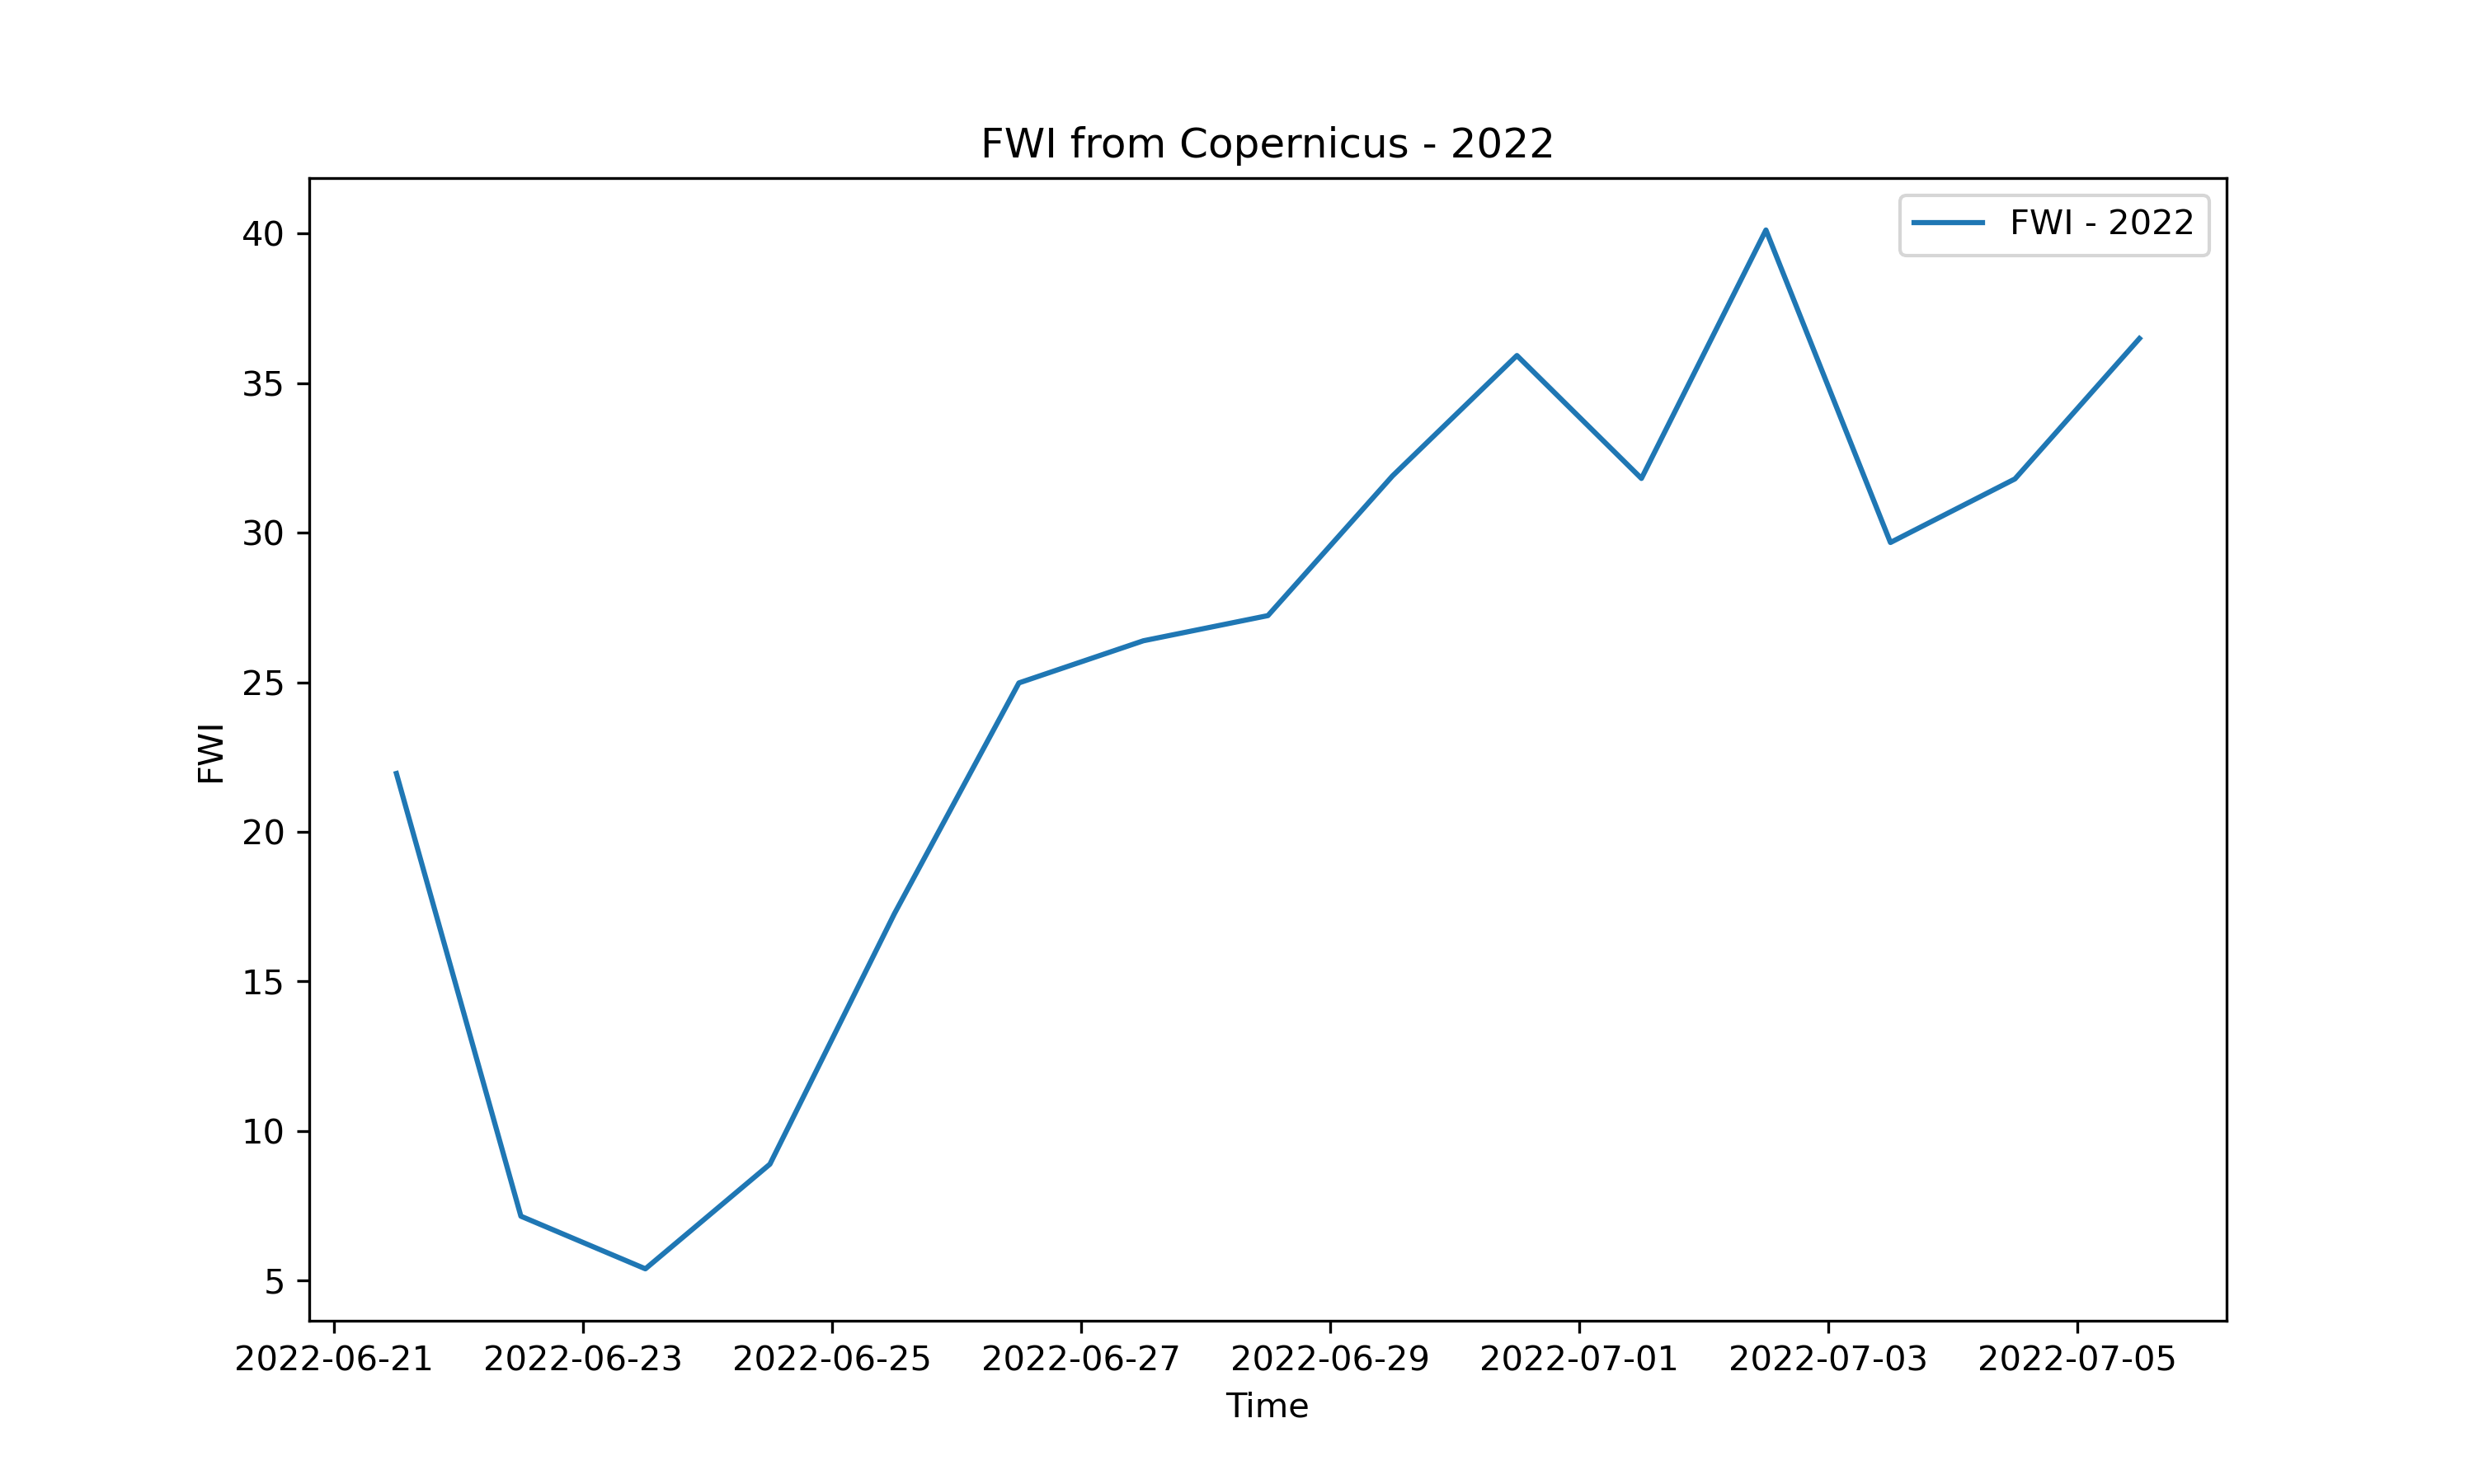
\includegraphics[width=\textwidth]{graphs/2022/2022CopernicusFWI12.png}
		\caption{FWI - Copernicus}
		\label{fig:fwi_copernicus_2022_midday}
	\end{subfigure}
	\hfill
	\begin{subfigure}{0.49\textwidth}
		\centering
		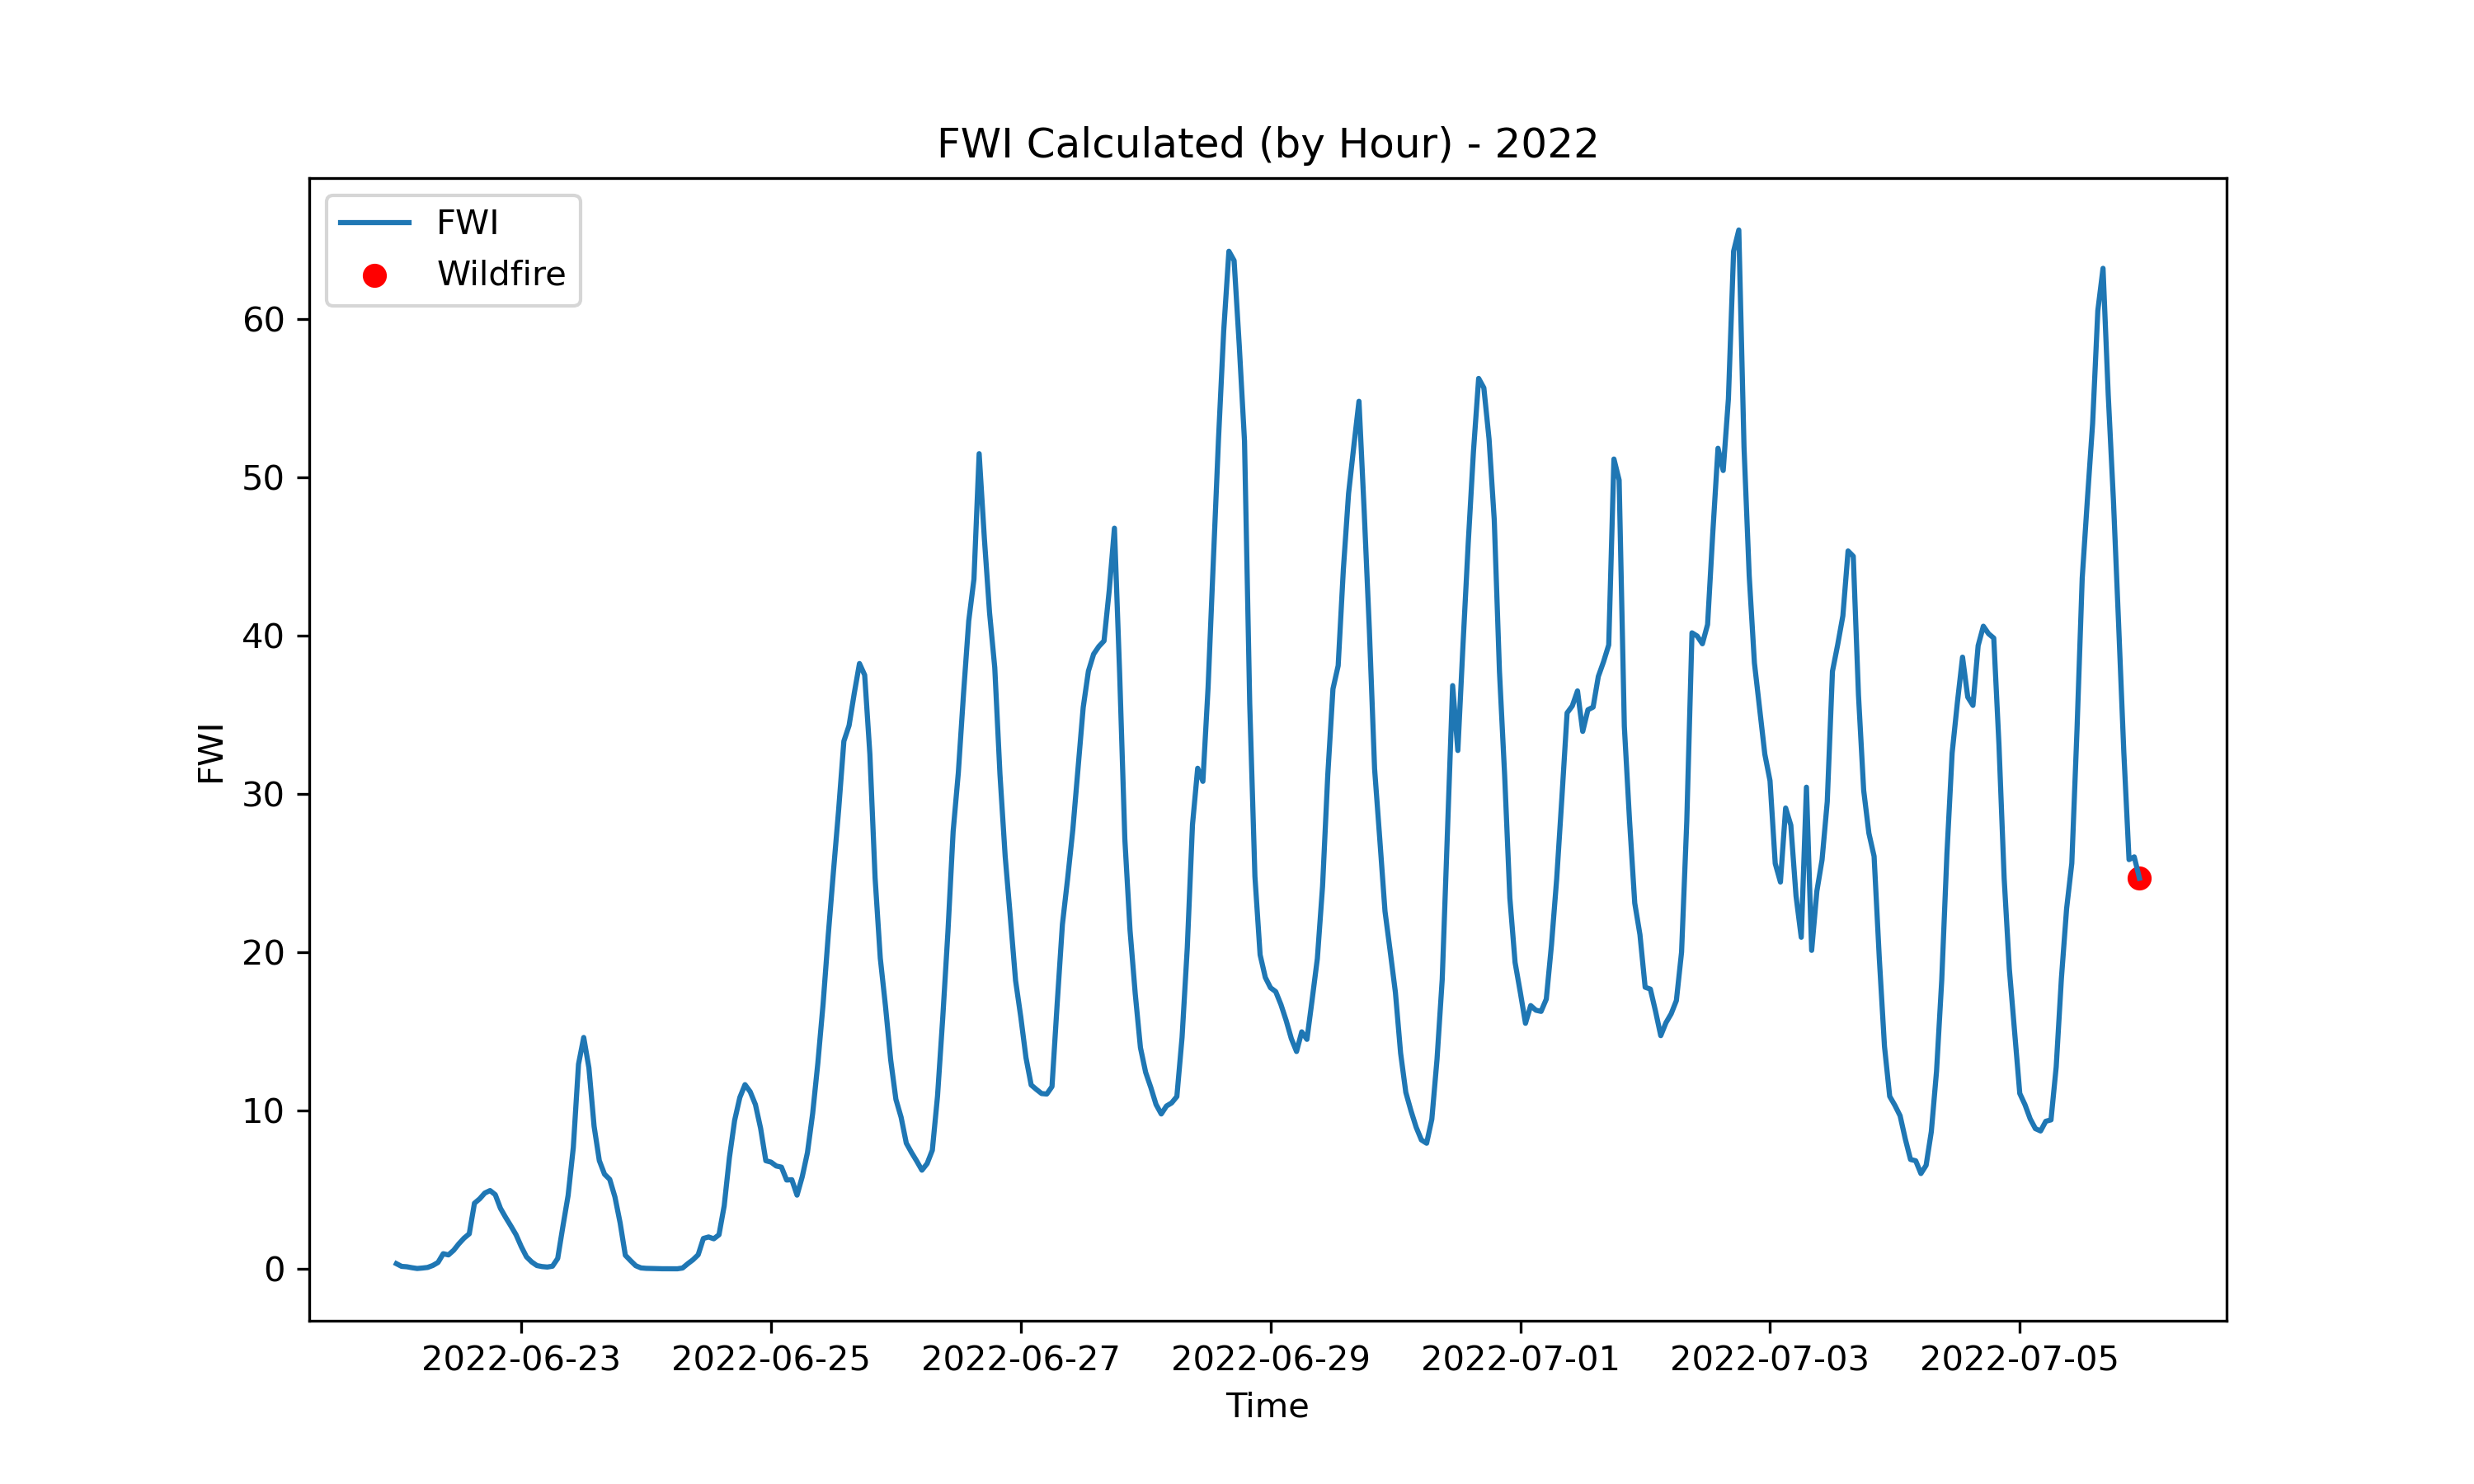
\includegraphics[width=\textwidth]{graphs/2022/2022CalcFWI12.png}
		\caption{FWI - Calculated value}
		\label{fig:fwi_calculated_2022_midday}
	\end{subfigure}
	\label{fig:comparison_fwi_2022_midday_copernicus_calculated}
\end{figure}

\FloatBarrier

\section{Hourly FWI variables}
\begin{figure}[h]
	\centering
	\caption{Calculated hourly FWI value for 2015, 2019, and 2022}
	\begin{subfigure}{0.45\textwidth}
		\centering
		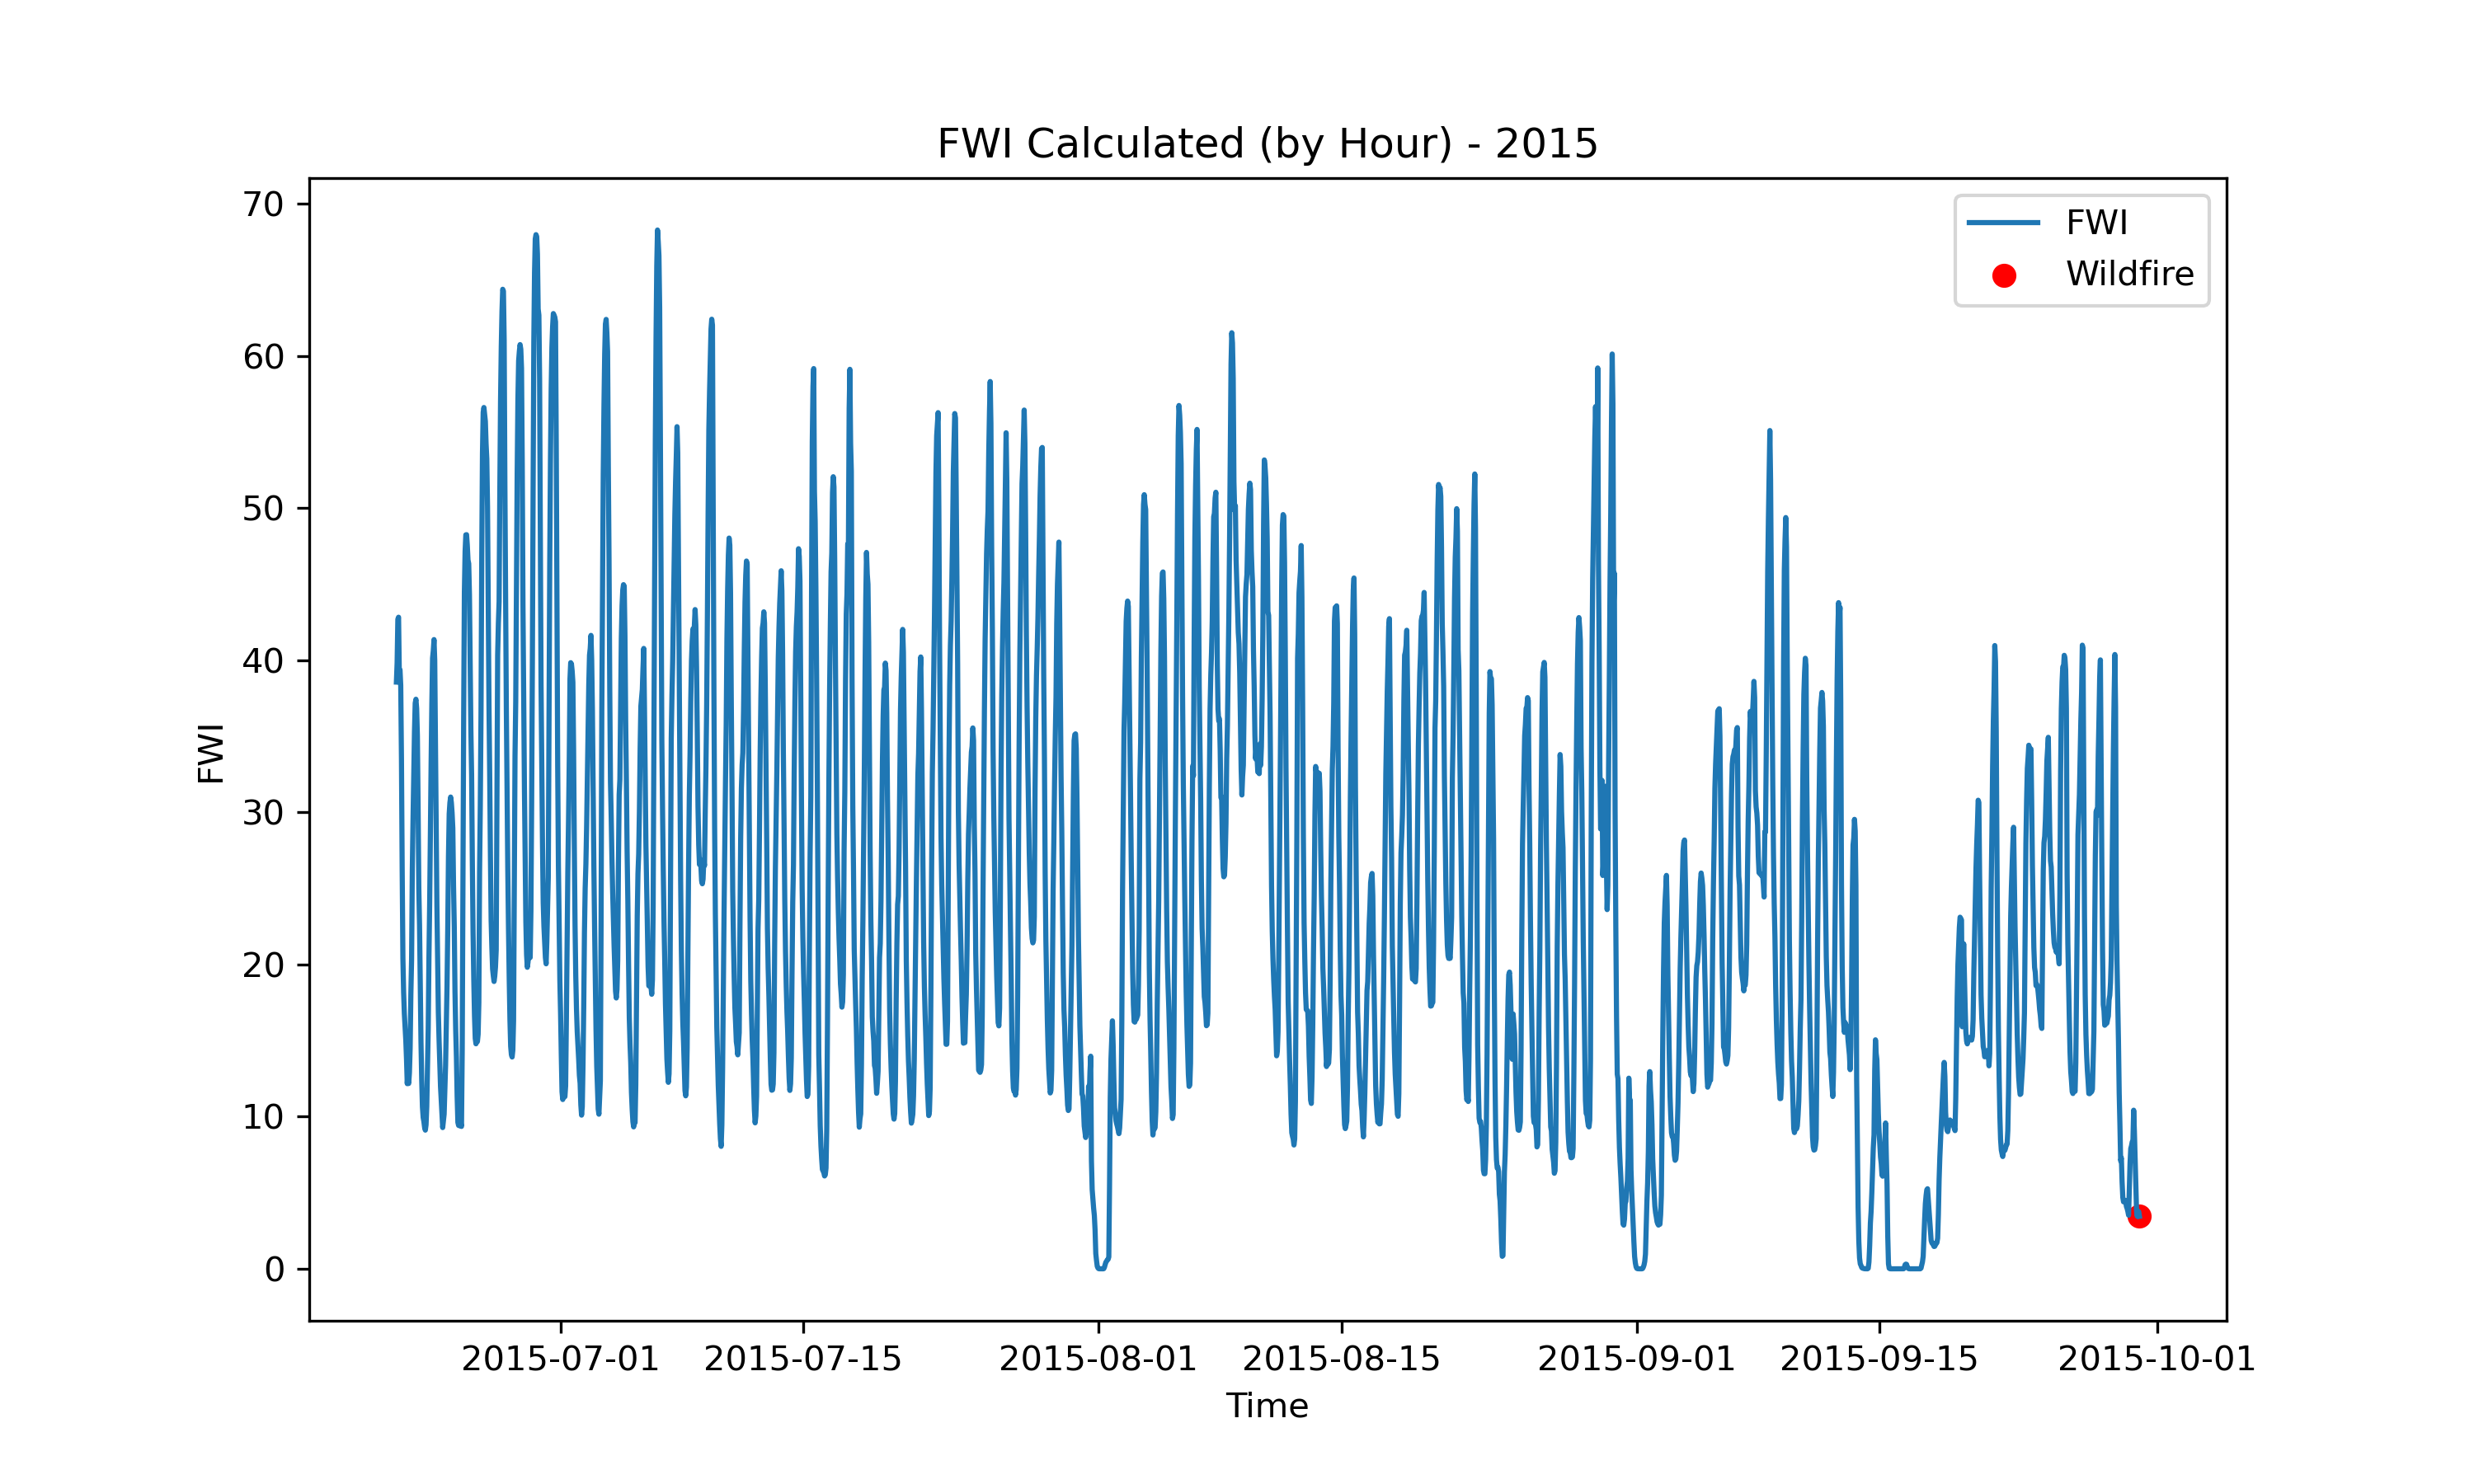
\includegraphics[width=\textwidth]{graphs/2015/byHour/2015CalcFWI12.png}
	\end{subfigure}
	\hfill
	\begin{subfigure}{0.45\textwidth}
		\centering
		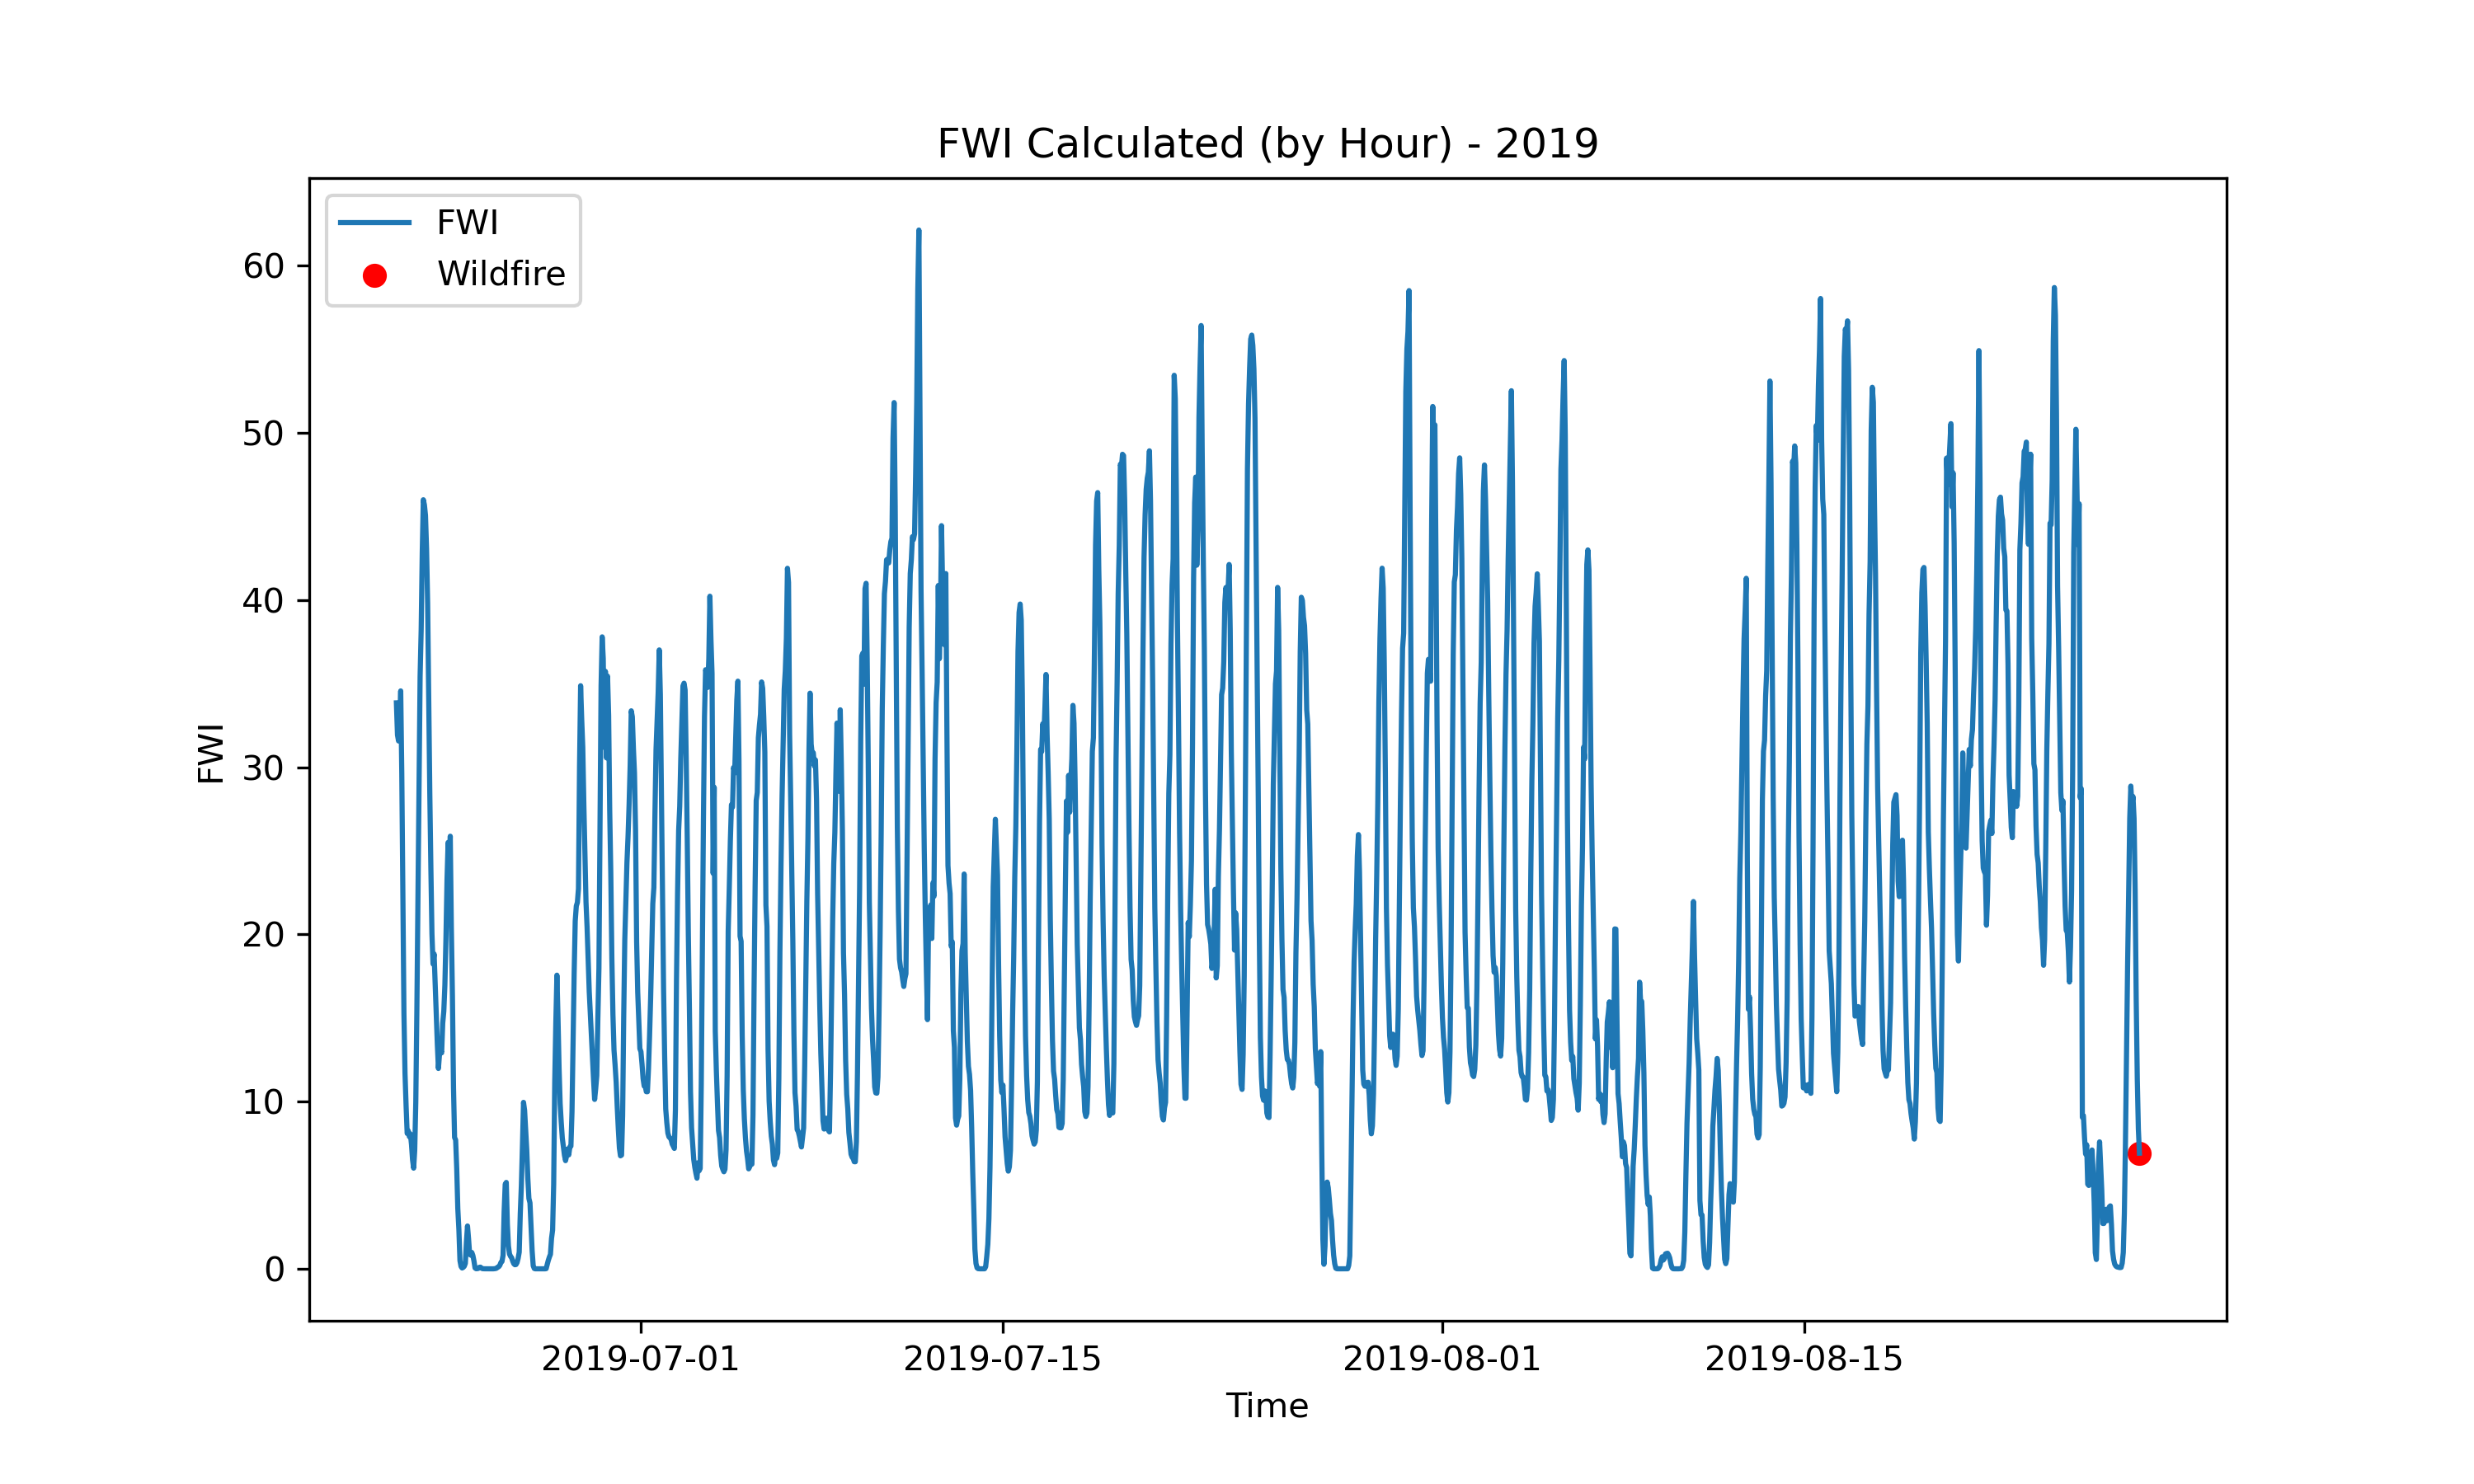
\includegraphics[width=\textwidth]{graphs/2019/byHour/2019CalcFWI12.png}
	\end{subfigure}
	
	\begin{subfigure}{0.45\textwidth}
		\centering
		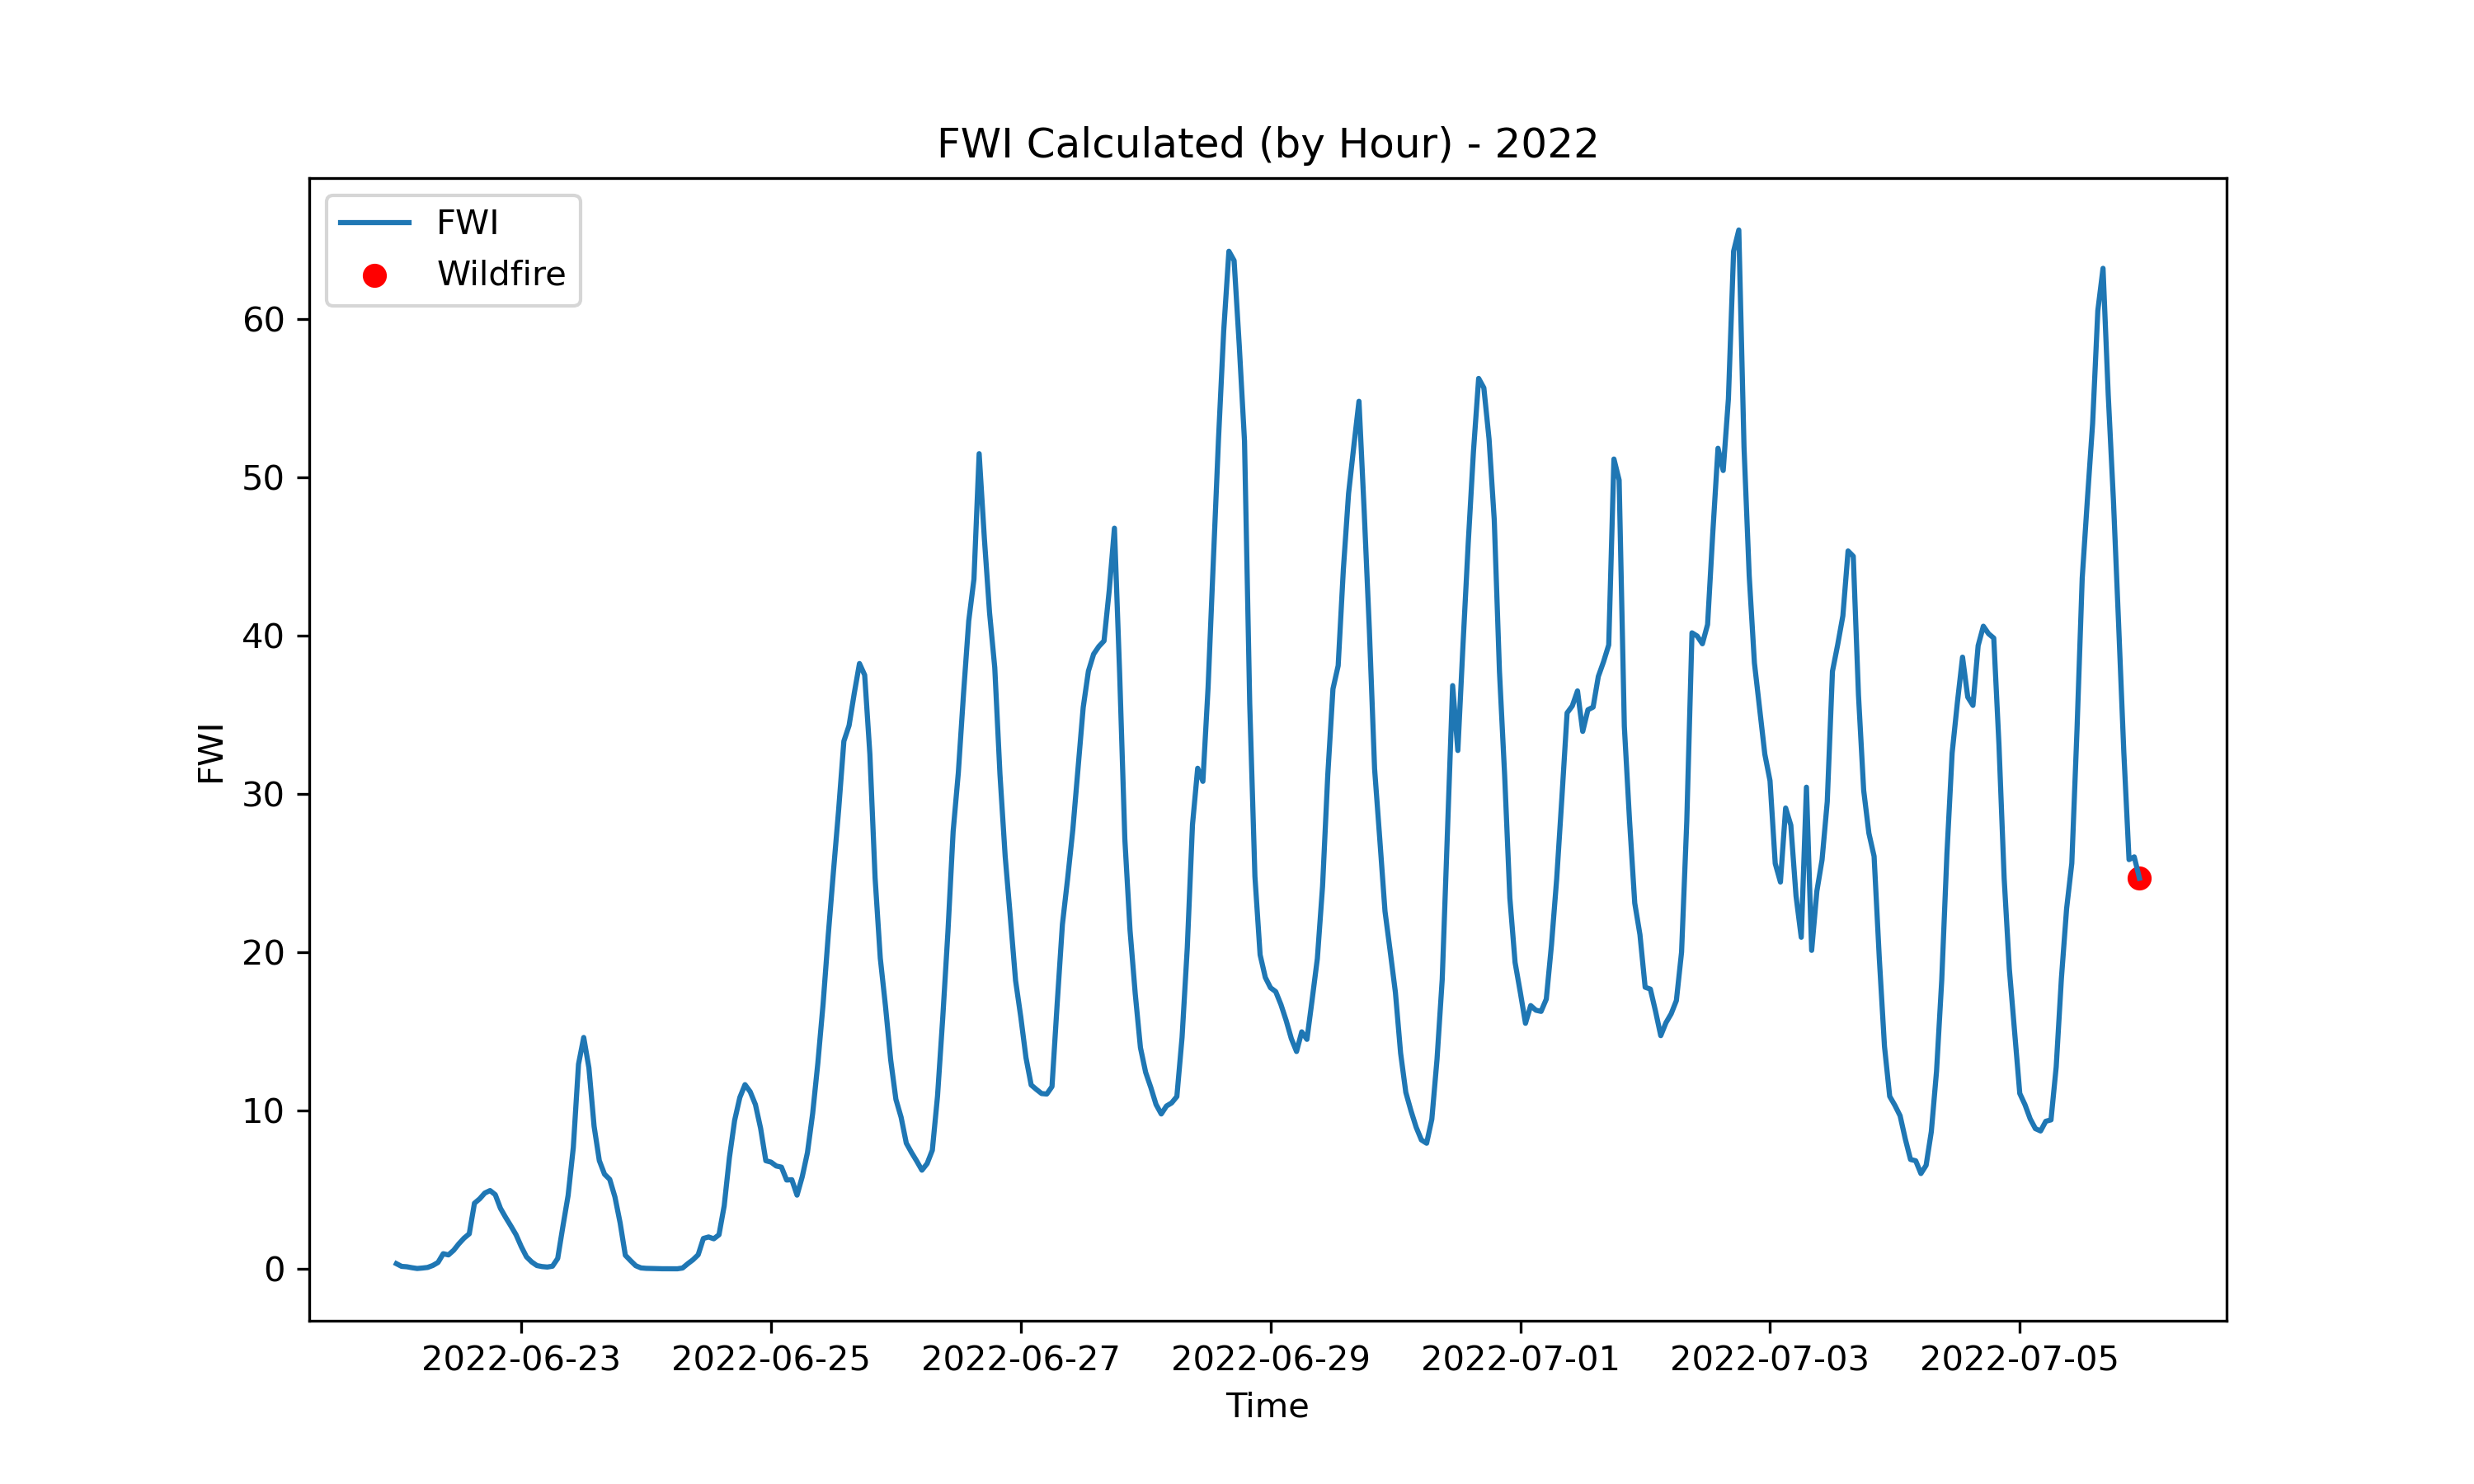
\includegraphics[width=\textwidth]{graphs/2022/2022CalcFWI12.png}
	\end{subfigure}
	
	\label{fig:hourly_fwi}
\end{figure}

\begin{figure}[h]
	\centering
	\caption{Calculated hourly FFMC value for 2015, 2019, and 2022}
	\begin{subfigure}{0.45\textwidth}
		\centering
		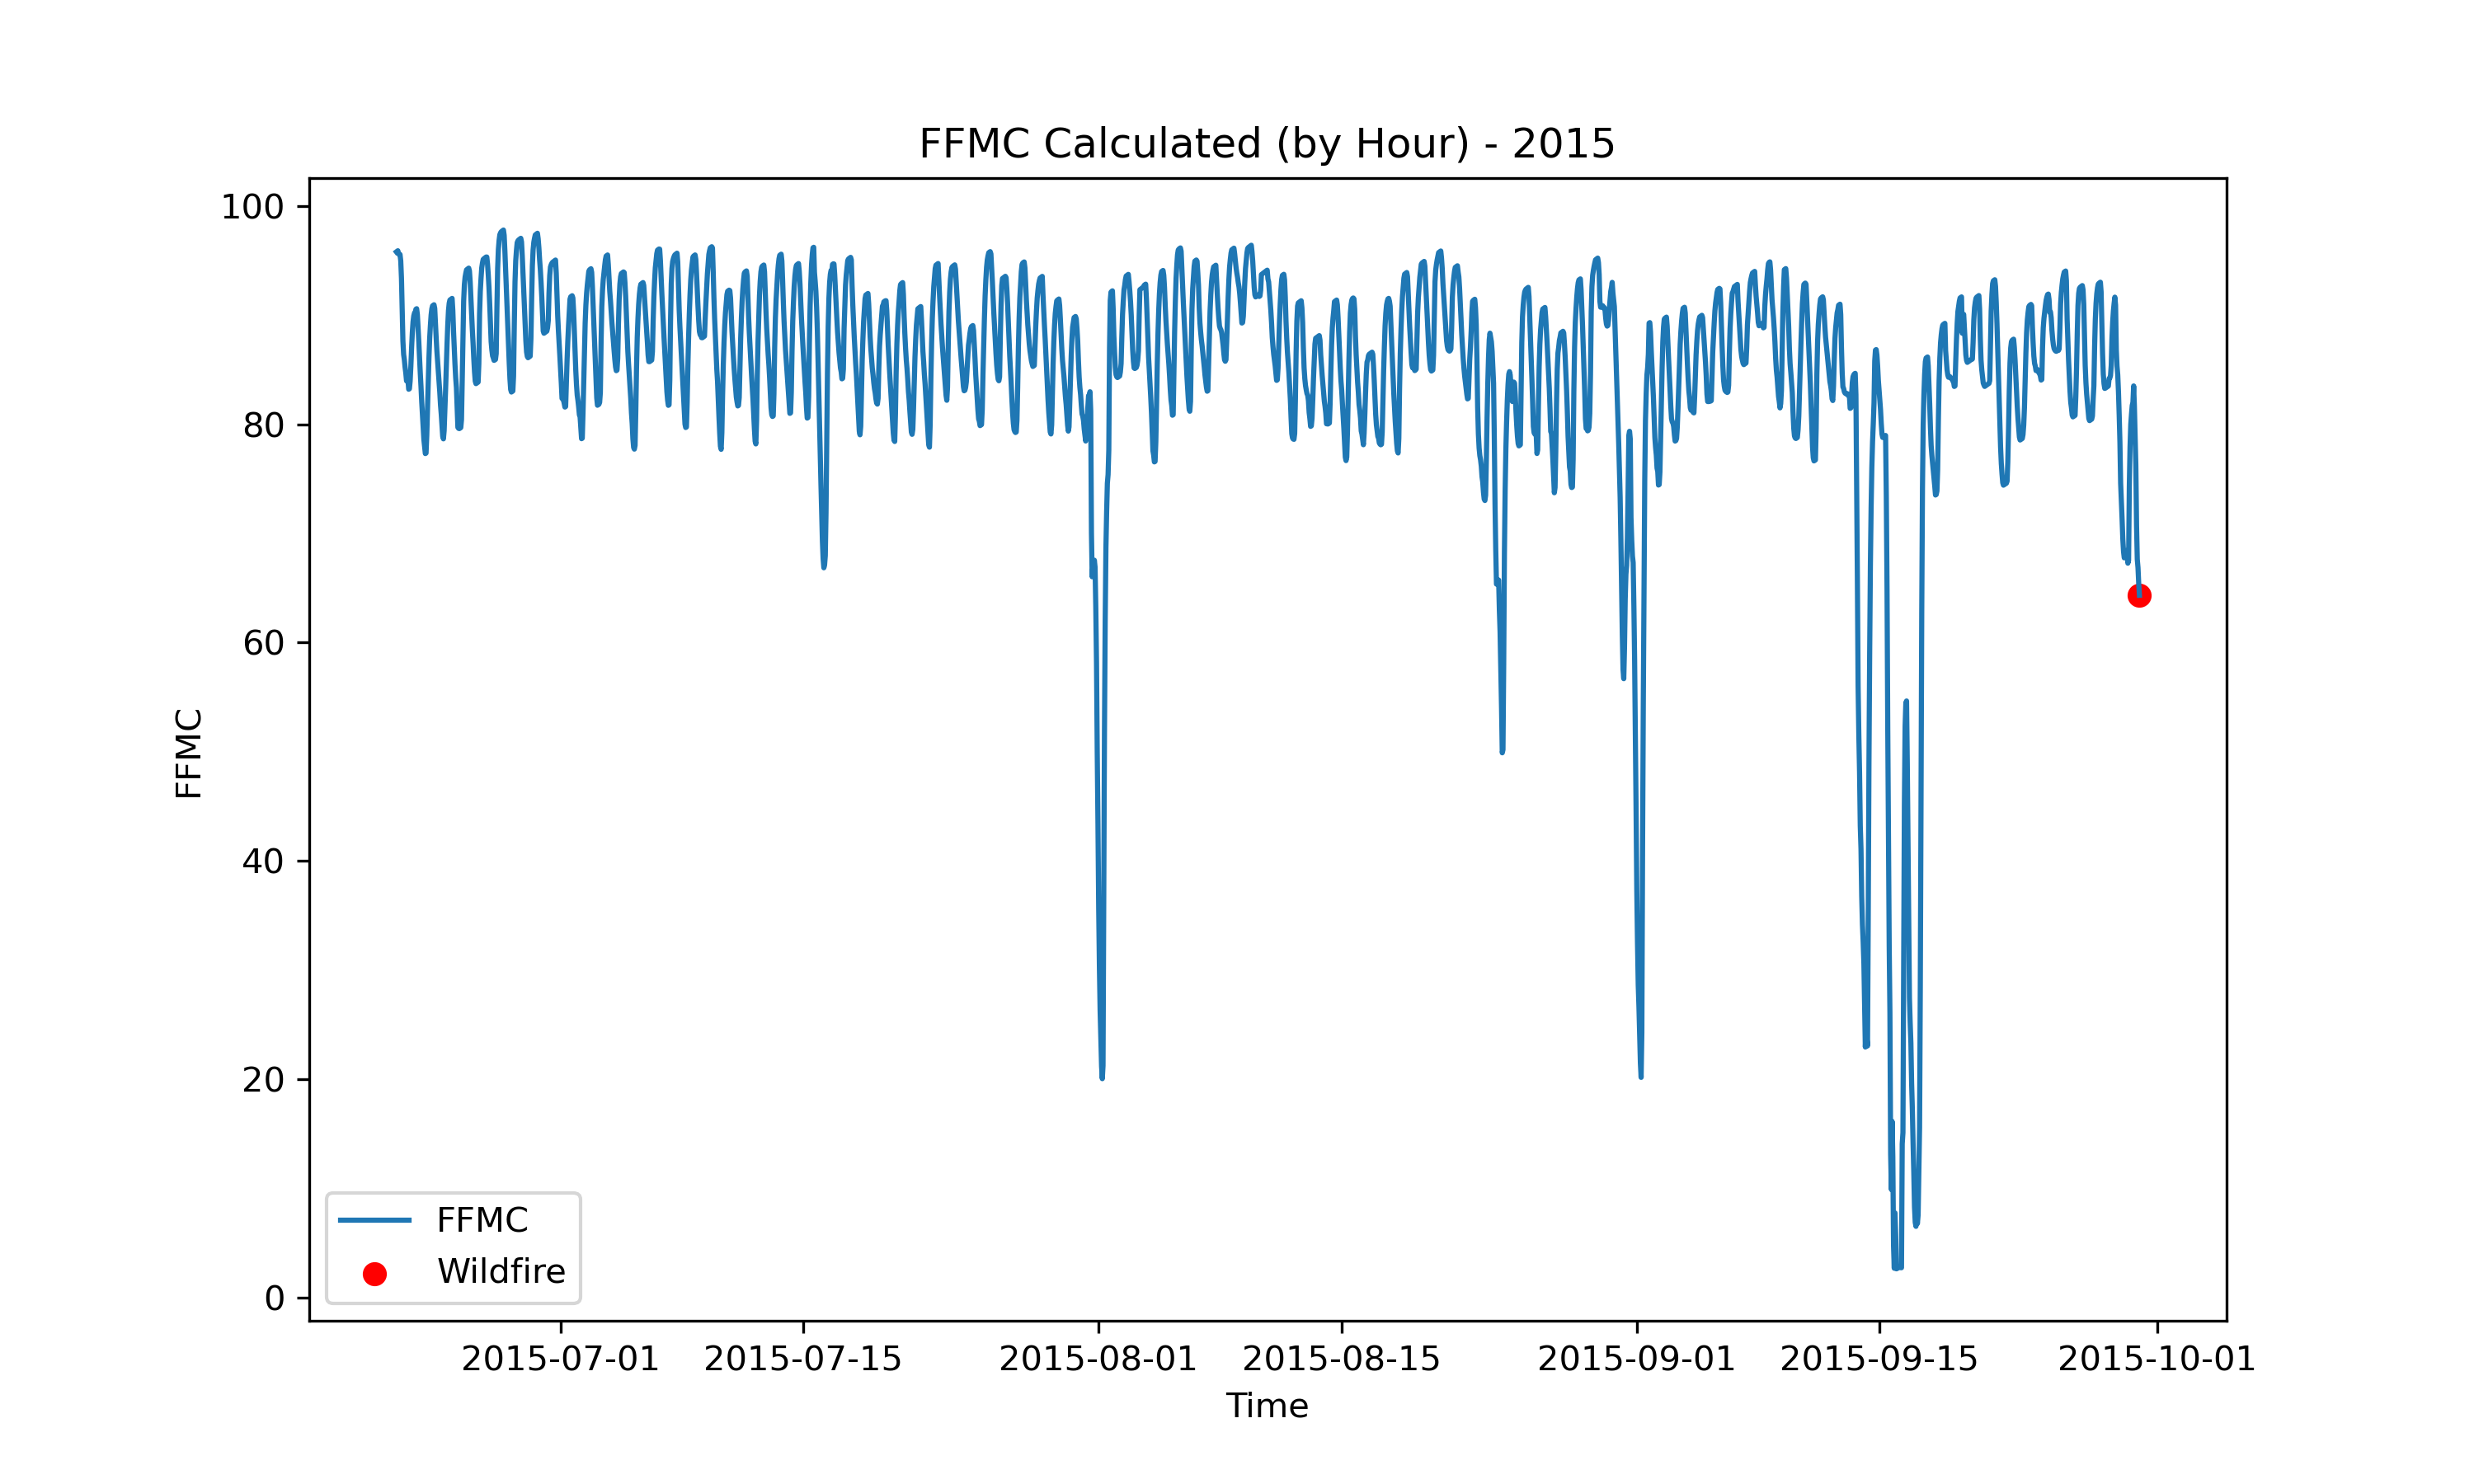
\includegraphics[width=\textwidth]{graphs/2015/byHour/2015CalcFFMC12.png}
	\end{subfigure}
	\hfill
	\begin{subfigure}{0.45\textwidth}
		\centering
		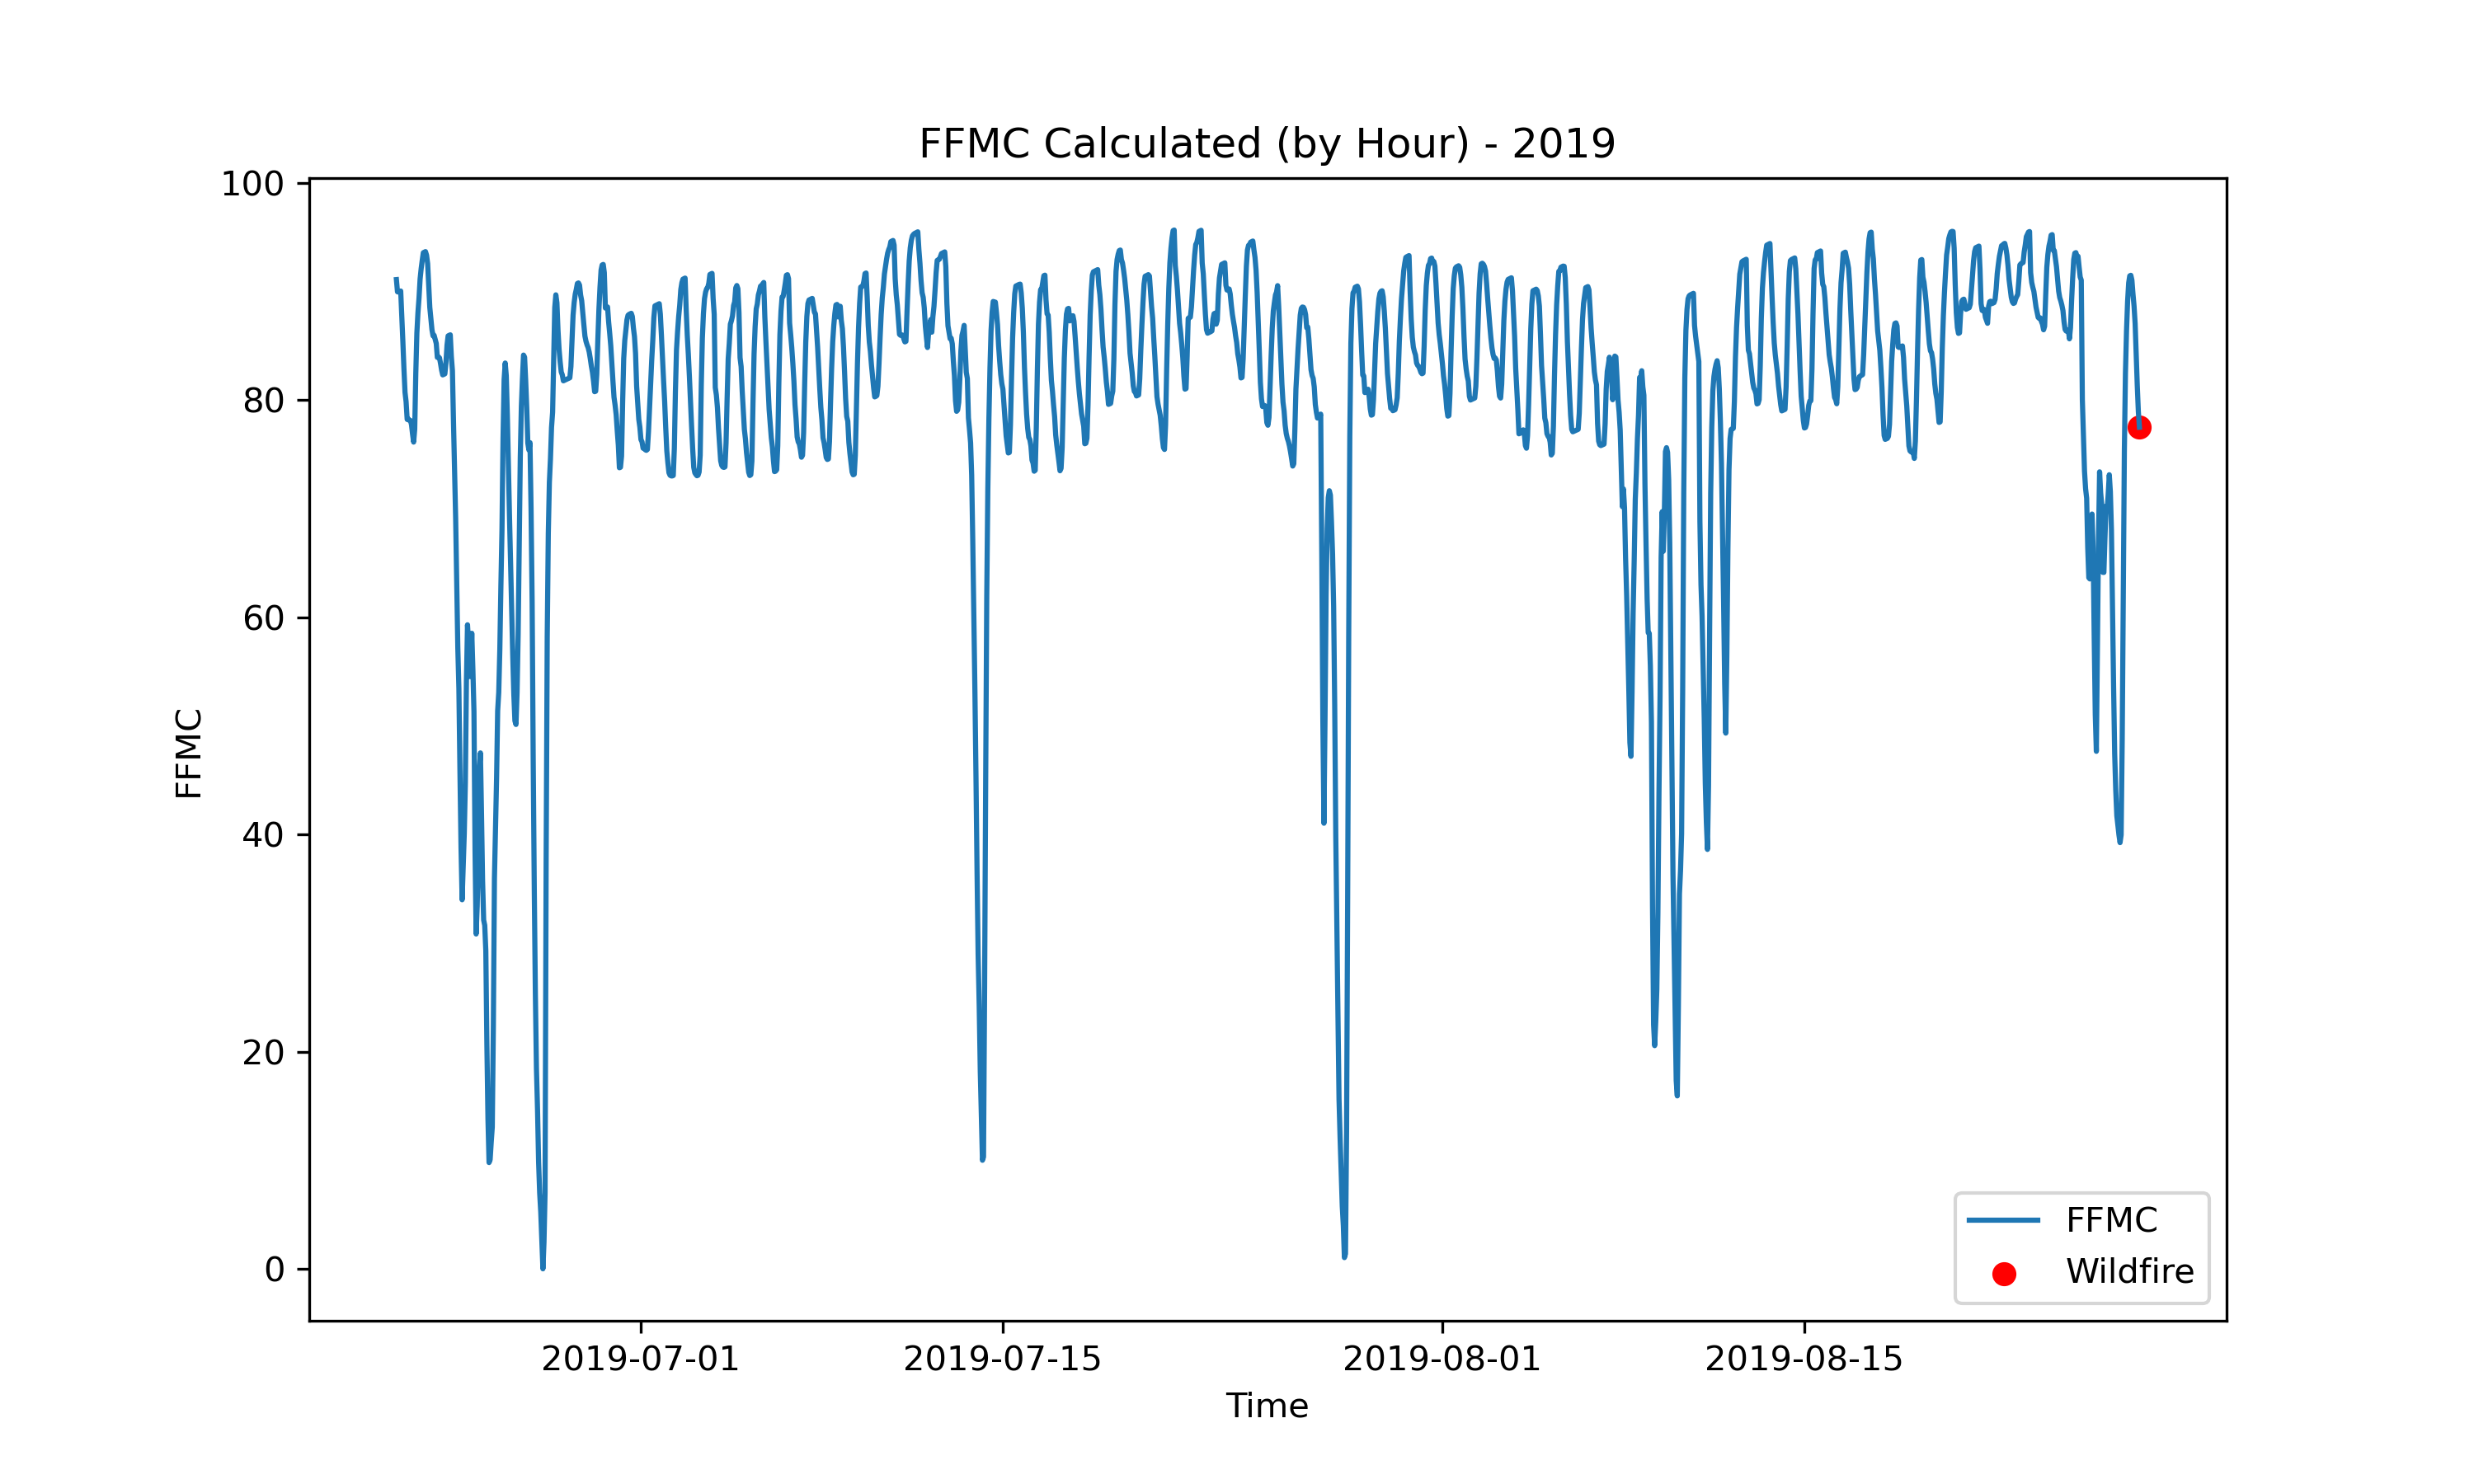
\includegraphics[width=\textwidth]{graphs/2019/2019CalcFFMC12.png}
	\end{subfigure}
	\hfill
	\begin{subfigure}{0.45\textwidth}
		\centering
		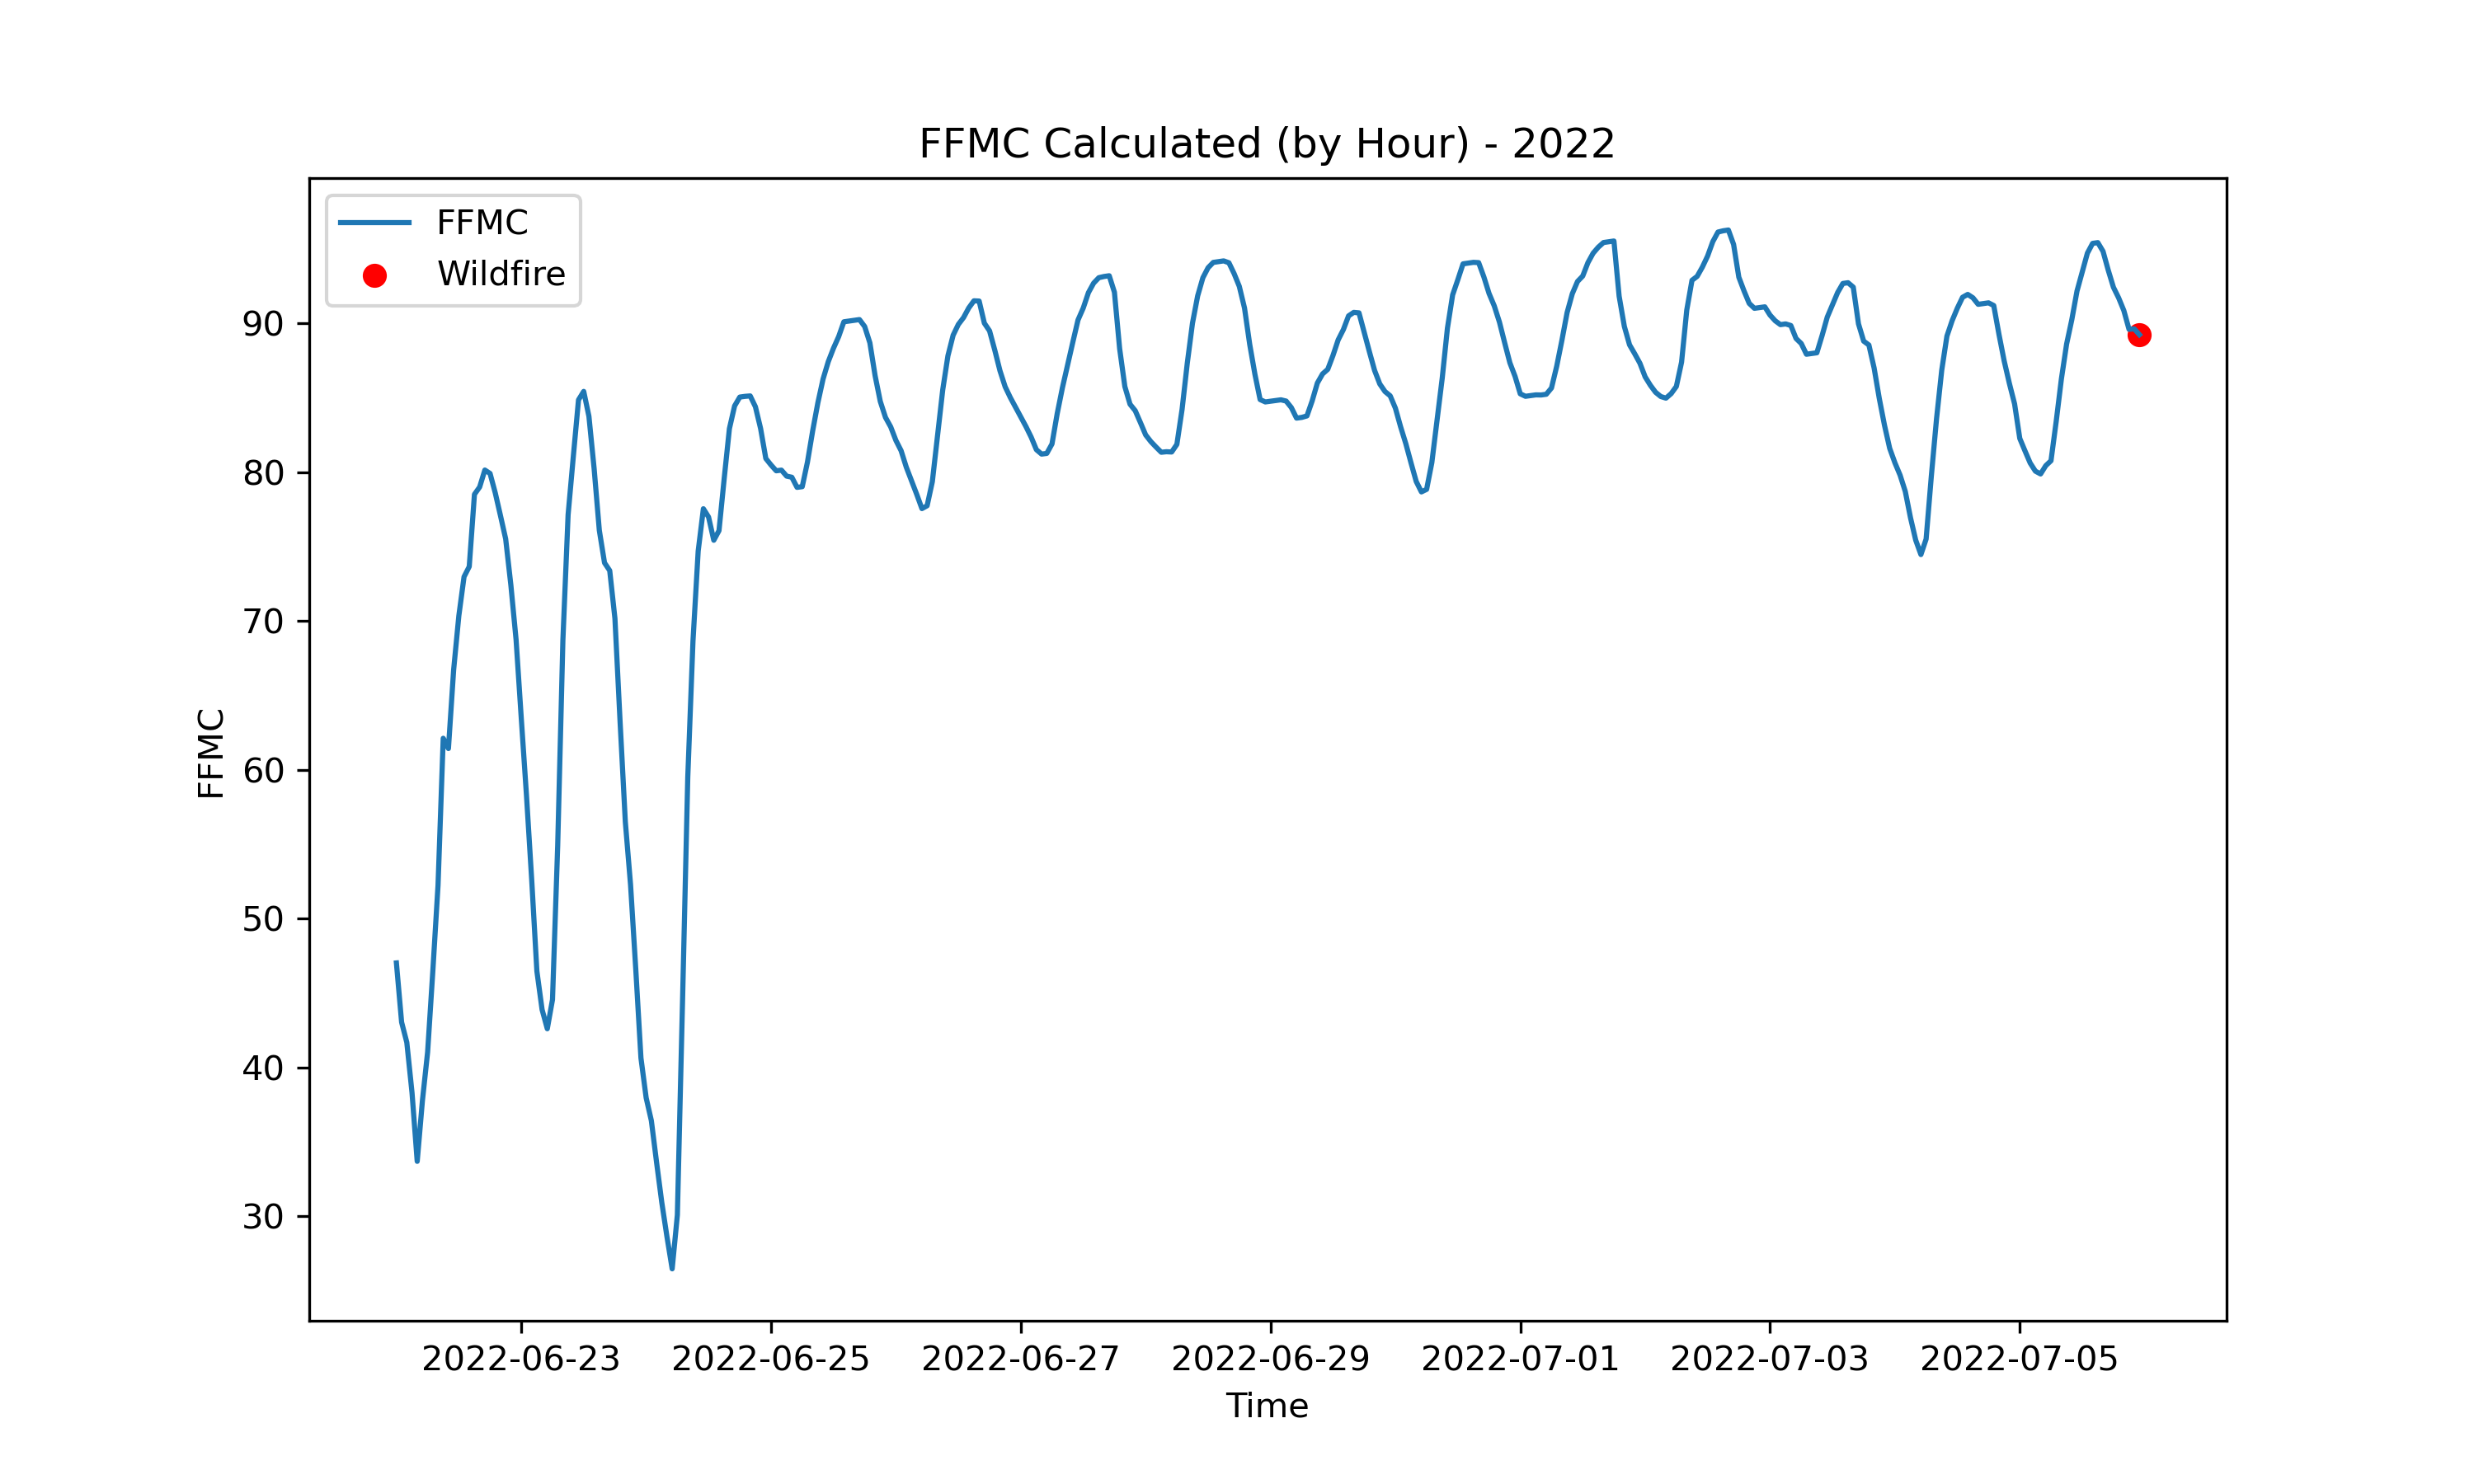
\includegraphics[width=\textwidth]{graphs/2022/2022CalcFFMC12.png}
	\end{subfigure}
	\label{fig:hourly_ffmc}
\end{figure}

\begin{figure}[h]
	\centering
	\caption{Calculated hourly DMC value for 2015, 2019, and 2022}
	\begin{subfigure}{0.45\textwidth}
		\centering
		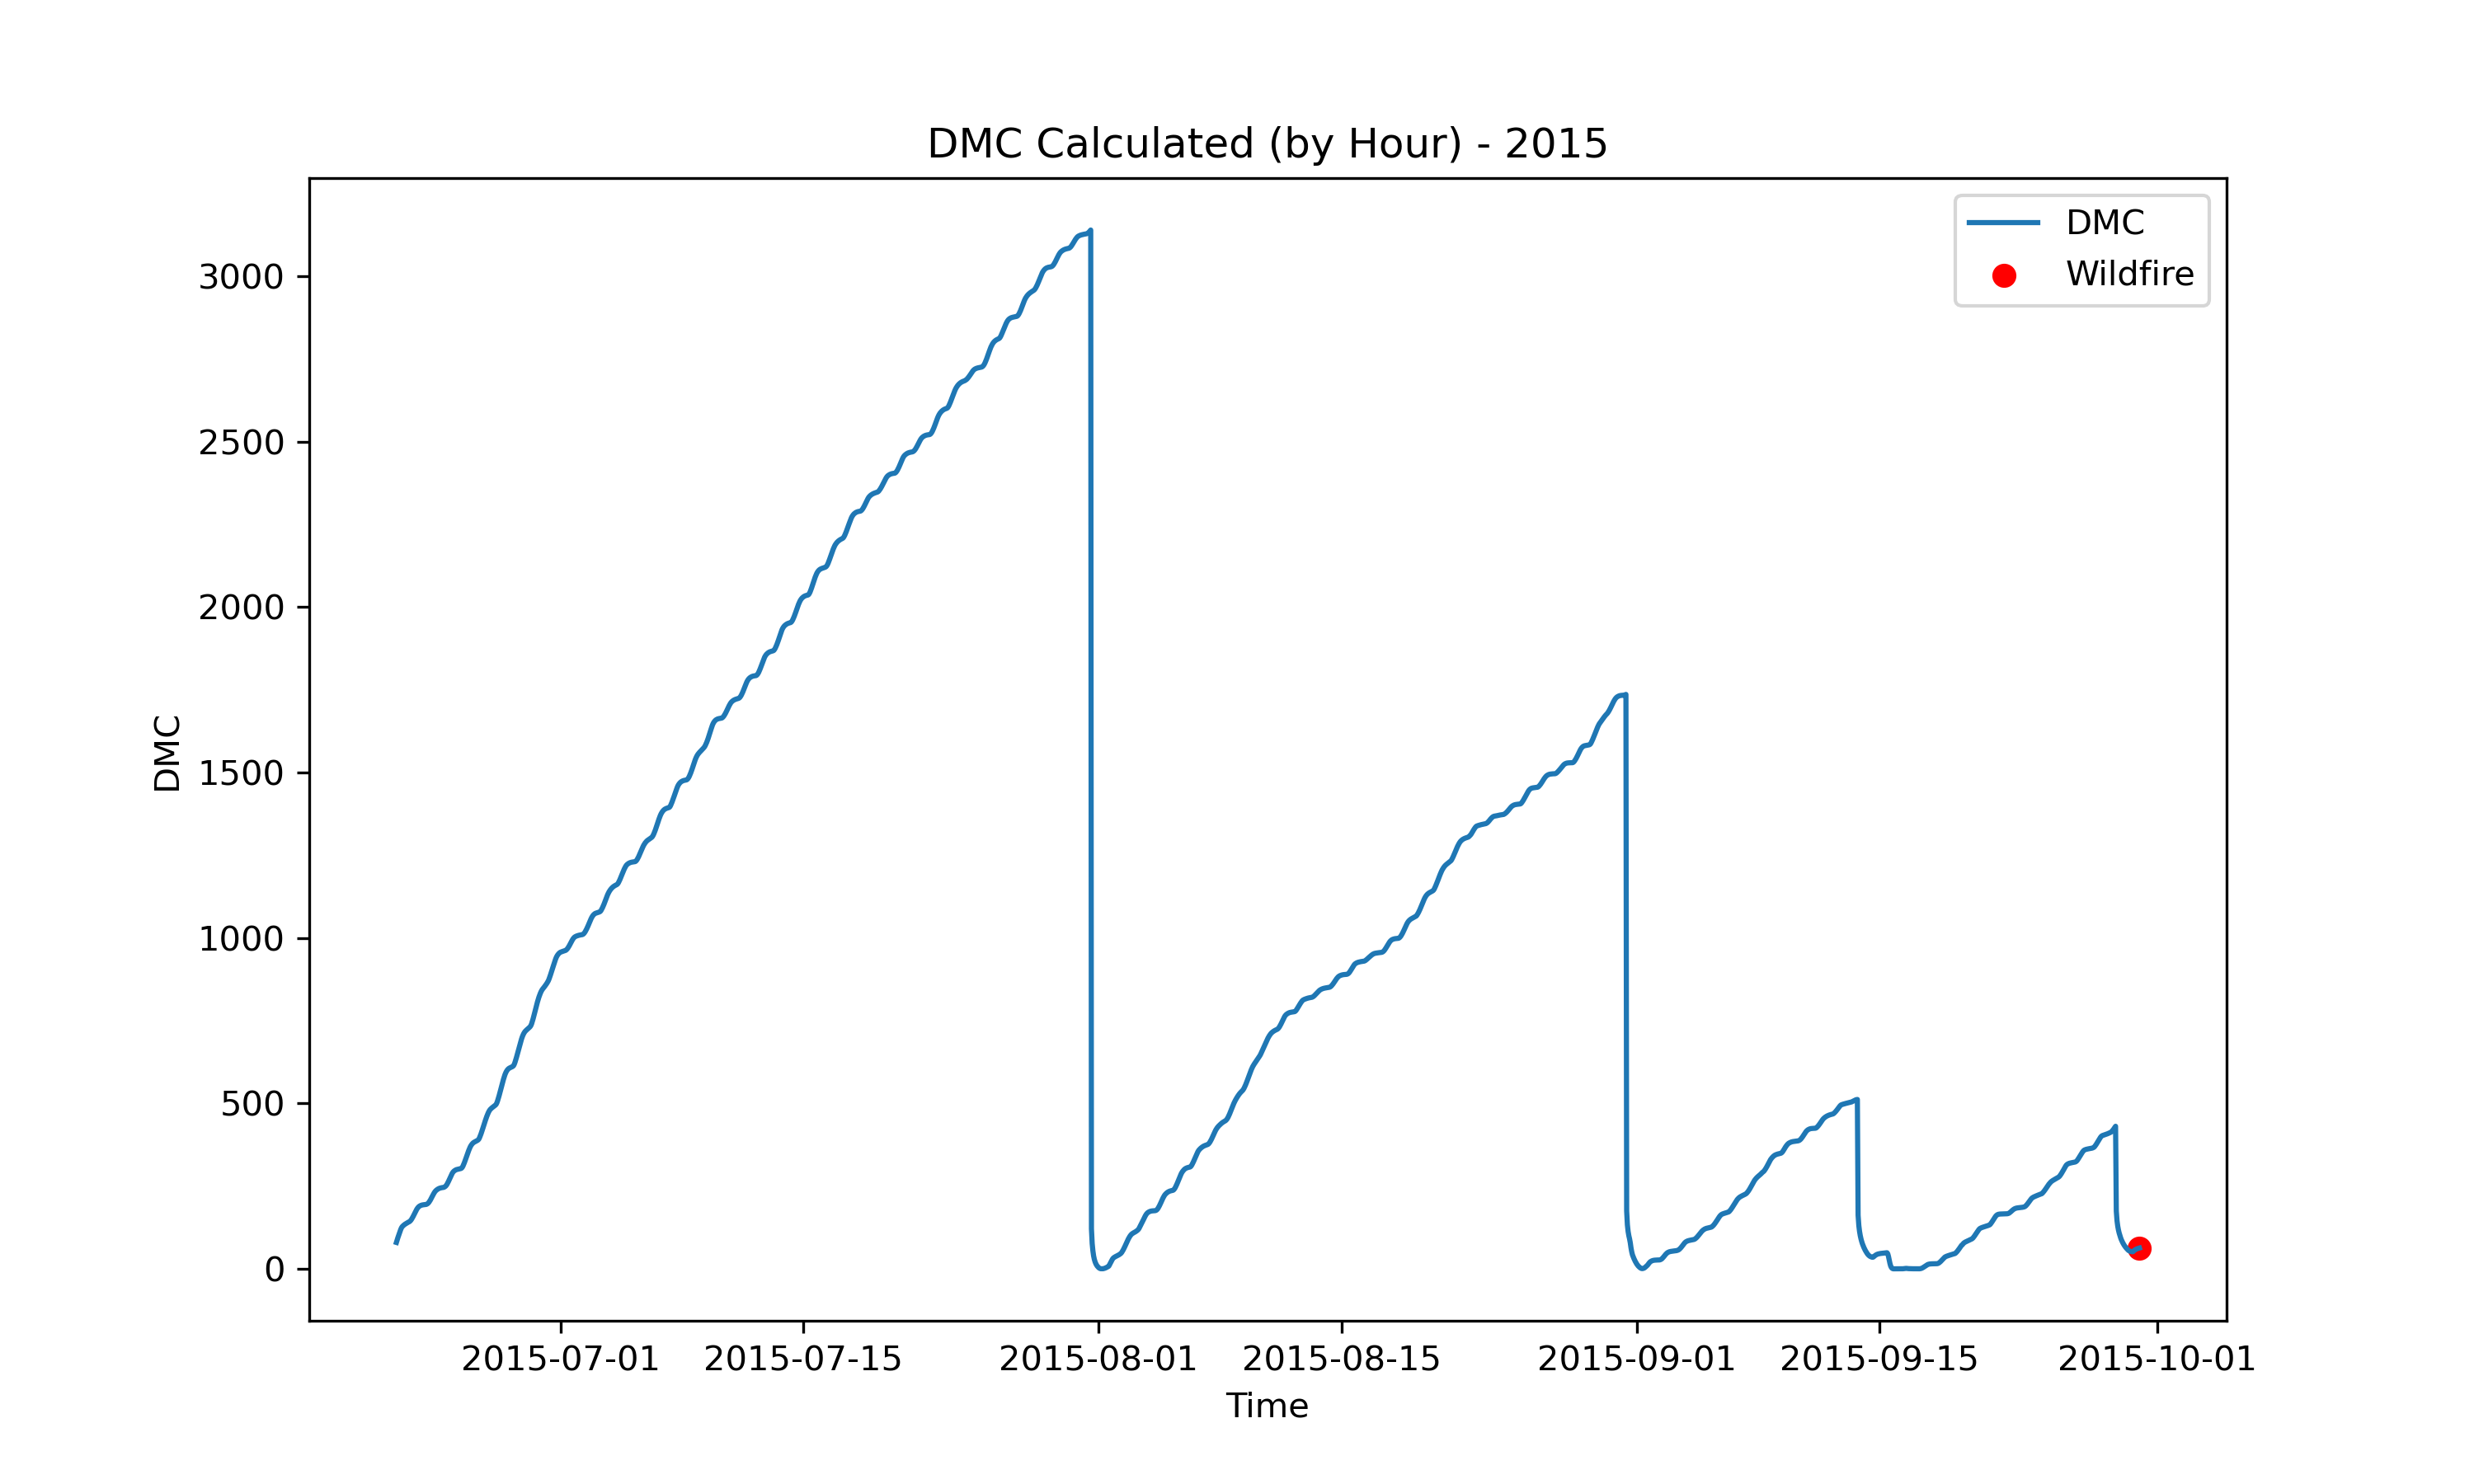
\includegraphics[width=\textwidth]{graphs/2015/byHour/2015CalcDMC12.png}
	\end{subfigure}
	\hfill
	\begin{subfigure}{0.45\textwidth}
		\centering
		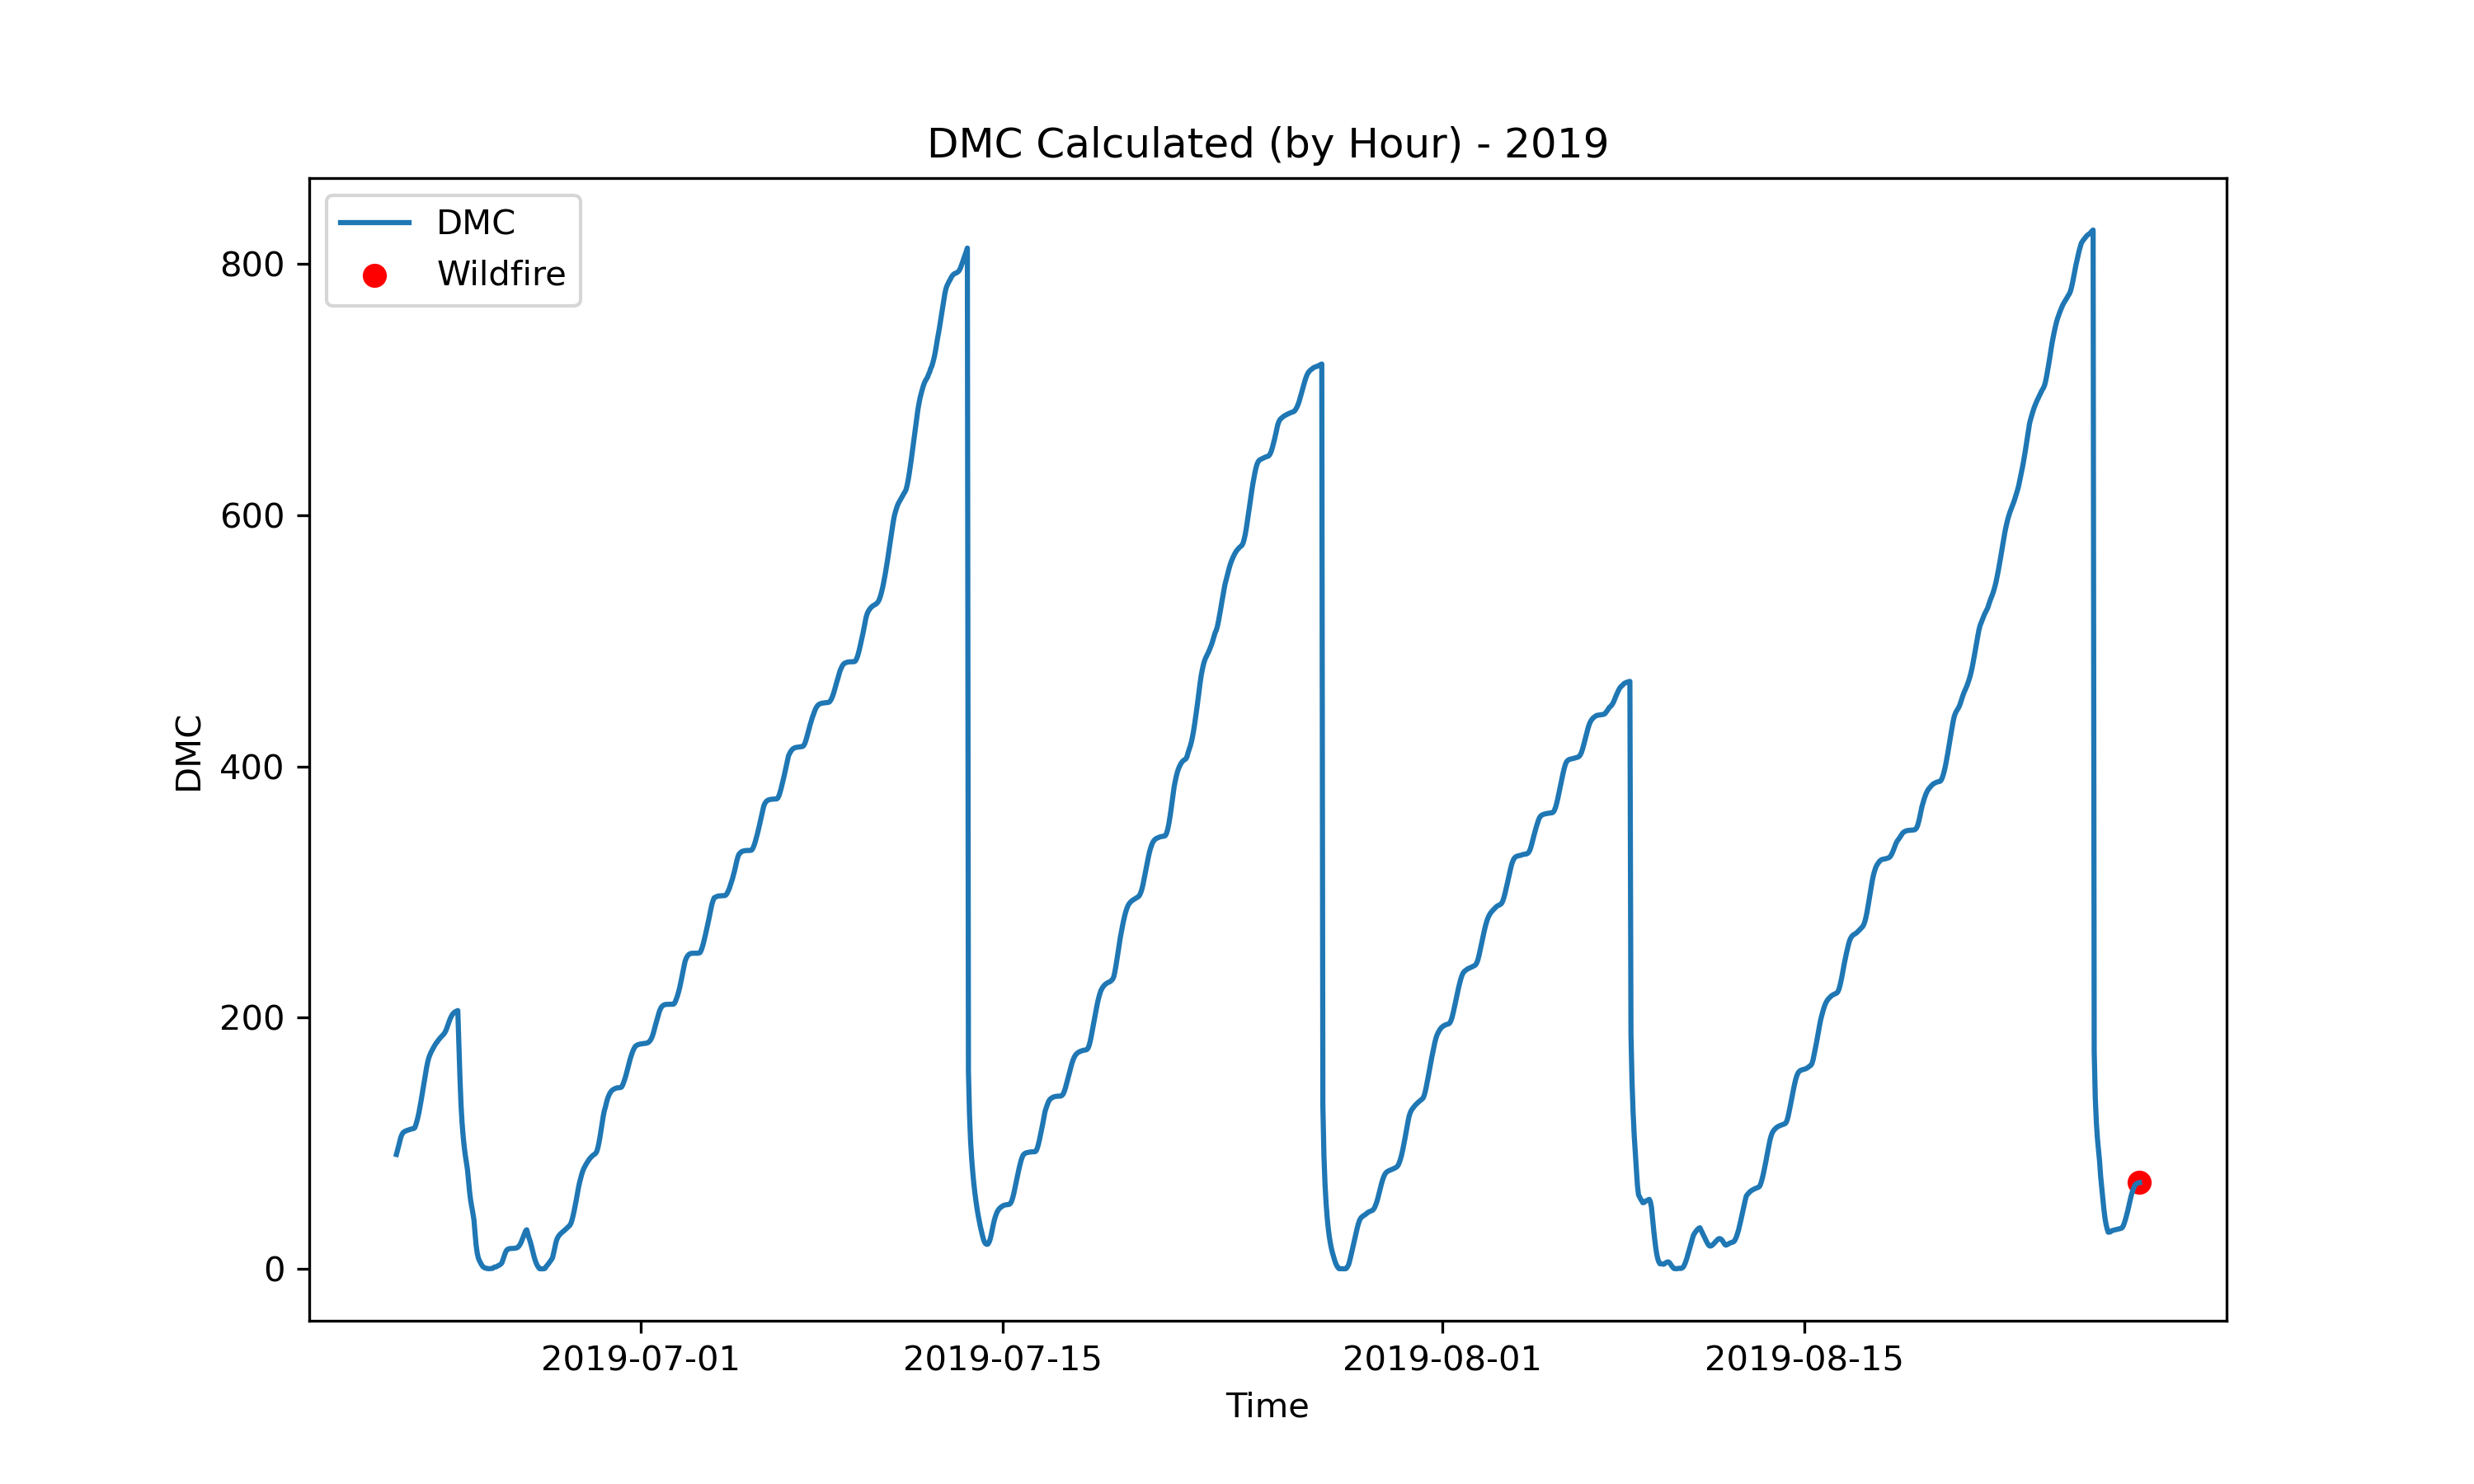
\includegraphics[width=\textwidth]{graphs/2019/2019CalcDMC12.png}
	\end{subfigure}
	\hfill
	\begin{subfigure}{0.45\textwidth}
		\centering
		\includegraphics[width=\textwidth]{graphs/2022/2022CalcDMC12.png}
	\end{subfigure}
	
	\label{fig:hourly_dmc}
\end{figure}

\begin{figure}[h]
	\centering
	\caption{Calculated hourly DC value for 2015, 2019, and 2022}
	\begin{subfigure}{0.45\textwidth}
		\centering
		\includegraphics[width=\textwidth]{graphs/2015/byHour/2015CalcDC12.png}
	\end{subfigure}
	\hfill
	\begin{subfigure}{0.45\textwidth}
		\centering
		\includegraphics[width=\textwidth]{graphs/2019/2019CalcDC12.png}
	\end{subfigure}
	\hfill
	\begin{subfigure}{0.45\textwidth}
		\centering
		\includegraphics[width=\textwidth]{graphs/2022/2022CalcDC12.png}
	\end{subfigure}
	\label{fig:hourly_dc}
\end{figure}

\begin{figure}[h]
	\centering
	\caption{Calculated hourly ISI value for 2015, 2019, and 2022}
	\begin{subfigure}{0.45\textwidth}
		\centering
		\includegraphics[width=\textwidth]{graphs/2015/byHour/2015CalcISI12.png}
	\end{subfigure}
	\hfill
	\begin{subfigure}{0.45\textwidth}
		\centering
		\includegraphics[width=\textwidth]{graphs/2019/2019CalcISI12.png}
	\end{subfigure}
	\hfill
	\begin{subfigure}{0.45\textwidth}
		\centering
		\includegraphics[width=\textwidth]{graphs/2022/2022CalcISI12.png}
	\end{subfigure}
	\label{fig:hourly_isi}
\end{figure}

\begin{figure}[h]
	\centering
	\caption{Calculated hourly BUI value for 2015, 2019, and 2022}
	\begin{subfigure}{0.45\textwidth}
		\centering
		\includegraphics[width=\textwidth]{graphs/2015/byHour/2015CalcBUI12.png}
	\end{subfigure}
	\hfill
	\begin{subfigure}{0.45\textwidth}
		\centering
		\includegraphics[width=\textwidth]{graphs/2019/2019CalcBUI12.png}
		\caption{Caption for image 2}
		\label{fig:img2}
	\end{subfigure}
	\hfill
	\begin{subfigure}{0.45\textwidth}
		\centering
		\includegraphics[width=\textwidth]{graphs/2022/2022CalcBUI12.png}
	\end{subfigure}
	
	\label{fig:hourly_bui}
\end{figure}

\FloatBarrier

\section{Evolution of maximum and minimum daily values of FWI variables}
\begin{figure}[h]
	\centering
	\caption{Daily max and min FWI values}
	\begin{subfigure}{0.45\textwidth}
		\centering
		\includegraphics[width=\textwidth]{graphs/2015/byHour/FWI_maxMin.png}
		\caption{2015}
	\end{subfigure}
	\hfill
	\begin{subfigure}{0.45\textwidth}
		\centering
		\includegraphics[width=\textwidth]{graphs/2019/byHour/FWI_maxMin.png}
		\caption{2019}
	\end{subfigure}
	\hfill
	\begin{subfigure}{0.45\textwidth}
		\centering
		\includegraphics[width=\textwidth]{graphs/2022/FWIX_maxMin.png}
		\caption{2022}
	\end{subfigure}
	
	\label{fig:daily_fwix_maxmin}
\end{figure}

\begin{figure}[h]
	\centering
	\caption{Daily max and min FFMC values}
	\begin{subfigure}{0.45\textwidth}
		\centering
		\includegraphics[width=\textwidth]{graphs/2015/byHour/FFMC_maxMin.png}
		\caption{2015}
	\end{subfigure}
	\hfill
	\begin{subfigure}{0.45\textwidth}
		\centering
		\includegraphics[width=\textwidth]{graphs/2019/byHour/FFMC_maxMin.png}
		\caption{2019}
	\end{subfigure}
	\hfill
	\begin{subfigure}{0.45\textwidth}
		\centering
		\includegraphics[width=\textwidth]{graphs/2022/FFMC_maxMin.png}
		\caption{2022}
	\end{subfigure}
	
	\label{fig:daily_ffmc_maxmin}
\end{figure}


\begin{figure}[h]
	\centering
	\caption{Daily max and min DMC values}
	\begin{subfigure}{0.45\textwidth}
		\centering
		\includegraphics[width=\textwidth]{graphs/2015/byHour/DMC_maxMin.png}
		\caption{2015}
	\end{subfigure}
	\hfill
	\begin{subfigure}{0.45\textwidth}
		\centering
		\includegraphics[width=\textwidth]{graphs/2019/byHour/DMC_maxMin.png}
		\caption{2019}
	\end{subfigure}
	\hfill
	\begin{subfigure}{0.45\textwidth}
		\centering
		\includegraphics[width=\textwidth]{graphs/2022/DMC_maxMin.png}
		\caption{2022}
	\end{subfigure}
	
	\label{fig:daily_dmc_maxmin}
\end{figure}

\begin{figure}[h]
	\centering
	\caption{Daily max and min DC values}
	\begin{subfigure}{0.45\textwidth}
		\centering
		\includegraphics[width=\textwidth]{graphs/2015/byHour/DC_maxMin.png}
		\caption{2015}
	\end{subfigure}
	\hfill
	\begin{subfigure}{0.45\textwidth}
		\centering
		\includegraphics[width=\textwidth]{graphs/2019/byHour/DC_maxMin.png}
		\caption{2019}
	\end{subfigure}
	\hfill
	\begin{subfigure}{0.45\textwidth}
		\centering
		\includegraphics[width=\textwidth]{graphs/2022/DC_maxMin.png}
		\caption{2022}
	\end{subfigure}
	
	\label{fig:daily_dc_maxmin}
\end{figure}

\begin{figure}[h]
	\centering
	\caption{Daily max and min ISI values}
	\begin{subfigure}{0.45\textwidth}
		\centering
		\includegraphics[width=\textwidth]{graphs/2015/byHour/ISI_maxMin.png}
		\caption{2015}
	\end{subfigure}
	\hfill
	\begin{subfigure}{0.45\textwidth}
		\centering
		\includegraphics[width=\textwidth]{graphs/2019/byHour/ISI_maxMin.png}
		\caption{2019}
	\end{subfigure}
	\hfill
	\begin{subfigure}{0.45\textwidth}
		\centering
		\includegraphics[width=\textwidth]{graphs/2022/ISI_maxMin.png}
		\caption{2022}
	\end{subfigure}
	\label{fig:daily_isi_maxmin}
\end{figure}

\begin{figure}[h]
	\centering
	\caption{Daily max and min BUI values}
	\begin{subfigure}{0.45\textwidth}
		\centering
		\includegraphics[width=\textwidth]{graphs/2015/byHour/BUI_maxMin.png}
		\caption{2015}
	\end{subfigure}
	\hfill
	\begin{subfigure}{0.45\textwidth}
		\centering
		\includegraphics[width=\textwidth]{graphs/2019/byHour/BUI_maxMin.png}
		\caption{2019}
	\end{subfigure}
	\hfill
	\begin{subfigure}{0.45\textwidth}
		\centering
		\includegraphics[width=\textwidth]{graphs/2022/BUI_maxMin.png}
		\caption{2022}
	\end{subfigure}
	\label{fig:daily_bui_maxmin}
\end{figure}

\FloatBarrier

\section{Before, after and daily maximum value}

\begin{figure}[h]
	\centering
	\caption{Before, after and daily FWI maximum value}
	\begin{subfigure}{0.45\textwidth}
		\centering
		\includegraphics[width=\textwidth]{graphs/2015/byHour/fwi_max_before_after.png}
		\caption{2015}
	\end{subfigure}
	\hfill
	\begin{subfigure}{0.45\textwidth}
		\centering
		\includegraphics[width=\textwidth]{graphs/2019/byHour/FWI_max_before_after.png}
		\caption{2019}
	\end{subfigure}
	\hfill
	\begin{subfigure}{0.45\textwidth}
		\centering
		\includegraphics[width=\textwidth]{graphs/2022/FWI_max_before_after.png}
		\caption{2022}
	\end{subfigure}
	\label{fig:daily_fwi_after_before_max}
\end{figure}

\begin{figure}[h]
	\centering
	\caption{Before, after and daily FFMC maximum value}
	\begin{subfigure}{0.45\textwidth}
		\centering
		\includegraphics[width=\textwidth]{graphs/2015/byHour/FFMC_max_before_after.png}
		\caption{2015}
	\end{subfigure}
	\hfill
	\begin{subfigure}{0.45\textwidth}
		\centering
		\includegraphics[width=\textwidth]{graphs/2019/byHour/FFMC_max_before_after.png}
		\caption{2019}
	\end{subfigure}
	\hfill
	\begin{subfigure}{0.45\textwidth}
		\centering
		\includegraphics[width=\textwidth]{graphs/2022/FFMC_max_before_after.png}
		\caption{2022}
	\end{subfigure}
	\label{fig:daily_ffmc_after_before_max}
\end{figure}

\begin{figure}[h]
	\centering
	\caption{Before, after and daily DMC maximum value}
	\begin{subfigure}{0.45\textwidth}
		\centering
		\includegraphics[width=\textwidth]{graphs/2015/byHour/DMC_max_before_after.png}
		\caption{2015}
	\end{subfigure}
	\hfill
	\begin{subfigure}{0.45\textwidth}
		\centering
		\includegraphics[width=\textwidth]{graphs/2019/byHour/DMC_max_before_after.png}
		\caption{2019}
	\end{subfigure}
	\hfill
	\begin{subfigure}{0.45\textwidth}
		\centering
		\includegraphics[width=\textwidth]{graphs/2022/DMC_max_before_after.png}
		\caption{2022}
	\end{subfigure}
	\label{fig:daily_dmc_after_before_max}
\end{figure}

\begin{figure}[h]
	\centering
	\caption{Before, after and daily DC maximum value}
	\begin{subfigure}{0.45\textwidth}
		\centering
		\includegraphics[width=\textwidth]{graphs/2015/byHour/DC_max_before_after.png}
		\caption{2015}
	\end{subfigure}
	\hfill
	\begin{subfigure}{0.45\textwidth}
		\centering
		\includegraphics[width=\textwidth]{graphs/2019/byHour/DC_max_before_after.png}
		\caption{2019}
	\end{subfigure}
	\hfill
	\begin{subfigure}{0.45\textwidth}
		\centering
		\includegraphics[width=\textwidth]{graphs/2022/DC_max_before_after.png}
		\caption{2022}
	\end{subfigure}
	\label{fig:daily_dc_after_before_max}
\end{figure}

\begin{figure}[h]
	\centering
	\caption{Before, after and daily ISI maximum value}
	\begin{subfigure}{0.45\textwidth}
		\centering
		\includegraphics[width=\textwidth]{graphs/2015/byHour/ISI_max_before_after.png}
		\caption{2015}
	\end{subfigure}
	\hfill
	\begin{subfigure}{0.45\textwidth}
		\centering
		\includegraphics[width=\textwidth]{graphs/2019/byHour/ISI_max_before_after.png}
		\caption{2019}
	\end{subfigure}
	\hfill
	\begin{subfigure}{0.45\textwidth}
		\centering
		\includegraphics[width=\textwidth]{graphs/2022/ISI_max_before_after.png}
		\caption{2022}
	\end{subfigure}
	\label{fig:daily_isi_after_before_max}
\end{figure}

\begin{figure}[h]
	\centering
	\caption{Before, after and daily BUI maximum value}
	\begin{subfigure}{0.45\textwidth}
		\centering
		\includegraphics[width=\textwidth]{graphs/2015/byHour/BUI_max_before_after.png}
		\caption{2015}
	\end{subfigure}
	\hfill
	\begin{subfigure}{0.45\textwidth}
		\centering
		\includegraphics[width=\textwidth]{graphs/2019/byHour/BUI_max_before_after.png}
		\caption{2019}
	\end{subfigure}
	\hfill
	\begin{subfigure}{0.45\textwidth}
		\centering
		\includegraphics[width=\textwidth]{graphs/2022/BUI_max_before_after.png}
		\caption{2022}
	\end{subfigure}
	\label{fig:daily_bui_after_before_max}
\end{figure}



\FloatBarrier

\section{Difference between the daily maximum and minimum values of the FWI variables}

\begin{figure}[h]
	\centering
	\caption{Daily difference of max and min FWI values}
	\begin{subfigure}{0.45\textwidth}
		\centering
		\includegraphics[width=\textwidth]{graphs/2015/byHour/FWI_DIFFmaxMin.png}
		\caption{2015}
	\end{subfigure}
	\hfill
	\begin{subfigure}{0.45\textwidth}
		\centering
		\includegraphics[width=\textwidth]{graphs/2019/byHour/FWI_DIFFmaxMin.png}
		\caption{2019}
	\end{subfigure}
	\hfill
	\begin{subfigure}{0.45\textwidth}
		\centering
		\includegraphics[width=\textwidth]{graphs/2022/FWIX_DIFFmaxMin.png}
		\caption{2022}
	\end{subfigure}
	\label{fig:daily_fwi_dif_maxmin}
\end{figure}

\begin{figure}[h]
	\centering
	\caption{Daily difference of max and min FFMC values}
	\begin{subfigure}{0.45\textwidth}
		\centering
		\includegraphics[width=\textwidth]{graphs/2015/byHour/FFMC_DIFFmaxMin.png}
		\caption{2015}
	\end{subfigure}
	\hfill
	\begin{subfigure}{0.45\textwidth}
		\centering
		\includegraphics[width=\textwidth]{graphs/2019/byHour/FFMC_DIFFmaxMin.png}
		\caption{2019}
	\end{subfigure}
	\hfill
	\begin{subfigure}{0.45\textwidth}
		\centering
		\includegraphics[width=\textwidth]{graphs/2022/FFMC_DIFFmaxMin.png}
		\caption{2022}
	\end{subfigure}
	\label{fig:daily_ffmc_dif_maxmin}
\end{figure}

\begin{figure}[h]
	\centering
	\caption{Daily difference of max and min DMC values}
	\begin{subfigure}{0.45\textwidth}
		\centering
		\includegraphics[width=\textwidth]{graphs/2015/byHour/DMC_DIFFmaxMin.png}
		\caption{2015}
	\end{subfigure}
	\hfill
	\begin{subfigure}{0.45\textwidth}
		\centering
		\includegraphics[width=\textwidth]{graphs/2019/byHour/DMC_DIFFmaxMin.png}
		\caption{2019}
	\end{subfigure}
	\hfill
	\begin{subfigure}{0.45\textwidth}
		\centering
		\includegraphics[width=\textwidth]{graphs/2022/DMC_DIFFmaxMin.png}
		\caption{2022}
	\end{subfigure}
	\label{fig:daily_dmc_dif_maxmin}
\end{figure}

\begin{figure}[h]
	\centering
	\caption{Daily difference of max and min DC values}
	\begin{subfigure}{0.45\textwidth}
		\centering
		\includegraphics[width=\textwidth]{graphs/2015/byHour/DC_DIFFmaxMin.png}
		\caption{2015}
	\end{subfigure}
	\hfill
	\begin{subfigure}{0.45\textwidth}
		\centering
		\includegraphics[width=\textwidth]{graphs/2019/byHour/DC_DIFFmaxMin.png}
		\caption{2019}
	\end{subfigure}
	\hfill
	\begin{subfigure}{0.45\textwidth}
		\centering
		\includegraphics[width=\textwidth]{graphs/2022/DC_DIFFmaxMin.png}
		\caption{2022}
	\end{subfigure}
	\label{fig:daily_dc_dif_maxmin}
\end{figure}

\begin{figure}[h]
	\centering
	\caption{Daily difference of max and min ISI values}
	\begin{subfigure}{0.45\textwidth}
		\centering
		\includegraphics[width=\textwidth]{graphs/2015/byHour/ISI_DIFFmaxMin.png}
		\caption{2015}
	\end{subfigure}
	\hfill
	\begin{subfigure}{0.45\textwidth}
		\centering
		\includegraphics[width=\textwidth]{graphs/2019/byHour/ISI_DIFFmaxMin.png}
		\caption{2019}
	\end{subfigure}
	\hfill
	\begin{subfigure}{0.45\textwidth}
		\centering
		\includegraphics[width=\textwidth]{graphs/2022/ISI_DIFFmaxMin.png}
		\caption{2022}
	\end{subfigure}
	\label{fig:daily_isi_dif_maxmin}
\end{figure}

\begin{figure}[h]
	\centering
	\caption{Daily difference of max and min BUI values}
	\begin{subfigure}{0.45\textwidth}
		\centering
		\includegraphics[width=\textwidth]{graphs/2015/byHour/BUI_DIFFmaxMin.png}
		\caption{2015}
	\end{subfigure}
	\hfill
	\begin{subfigure}{0.45\textwidth}
		\centering
		\includegraphics[width=\textwidth]{graphs/2019/byHour/BUI_DIFFmaxMin.png}
		\caption{2019}
	\end{subfigure}
	\hfill
	\begin{subfigure}{0.45\textwidth}
		\centering
		\includegraphics[width=\textwidth]{graphs/2022/BUI_DIFFmaxMin.png}
		\caption{2022}
	\end{subfigure}
	\label{fig:daily_bui_dif_maxmin}
\end{figure}


\FloatBarrier

\section{3-day time frame mean tendency graphs of FWI variables}
\begin{figure}[h]
	\caption{FWI mean tendency graph}
	\centering
	\begin{subfigure}{0.49\textwidth}
		\centering
		\includegraphics[width=\textwidth]{graphs/all_time/2015_tendency_graph_FWI.png}
		\caption{2015}
		\label{fig:mean_tendency_fwi_2015}
	\end{subfigure}
	\hfill
	\begin{subfigure}{0.49\textwidth}
		\centering
		\includegraphics[width=\textwidth]{graphs/all_time/2019_tendency_graph_FWI.png}
		\caption{2019}
		\label{fig:mean_tendency_fwi_2019}
	\end{subfigure}
	\label{fig:mean_tendency_fwi}
\end{figure}

\begin{figure}[h]
	\caption{FFMC mean tendency graph}
	\centering
	\begin{subfigure}{0.49\textwidth}
		\centering
		\includegraphics[width=\textwidth]{graphs/all_time/2015_tendency_graph_FFMC.png}
		\caption{2015}
		\label{fig:mean_tendency_ffmc_2015}
	\end{subfigure}
	\hfill
	\begin{subfigure}{0.49\textwidth}
		\centering
		\includegraphics[width=\textwidth]{graphs/all_time/2019_tendency_graph_FFMC.png}
		\caption{2019}
		\label{fig:mean_tendency_ffmc_2019}
	\end{subfigure}
	\label{fig:mean_tendency_ffmc}
\end{figure}

\begin{figure}[h]
	\caption{DMC mean tendency graph}
	\centering
	\begin{subfigure}{0.49\textwidth}
		\centering
		\includegraphics[width=\textwidth]{graphs/all_time/2015_tendency_graph_DMC.png}
		\caption{2015}
		\label{fig:mean_tendency_dmc_2015}
	\end{subfigure}
	\hfill
	\begin{subfigure}{0.49\textwidth}
		\centering
		\includegraphics[width=\textwidth]{graphs/all_time/2019_tendency_graph_DMC.png}
		\caption{2019}
		\label{fig:mean_tendency_dmc_2019}
	\end{subfigure}
	\label{fig:mean_tendency_dmc}
\end{figure}

\begin{figure}[h]
	\caption{DC mean tendency graph}
	\centering
	\begin{subfigure}{0.49\textwidth}
		\centering
		\includegraphics[width=\textwidth]{graphs/all_time/2015_tendency_graph_DC.png}
		\caption{2015}
		\label{fig:mean_tendency_dc_2015}
	\end{subfigure}
	\hfill
	\begin{subfigure}{0.49\textwidth}
		\centering
		\includegraphics[width=\textwidth]{graphs/all_time/2019_tendency_graph_DC.png}
		\caption{2019}
		\label{fig:mean_tendency_dc_2019}
	\end{subfigure}
	\label{fig:mean_tendency_dc}
\end{figure}

\begin{figure}[h]
	\caption{ISI mean tendency graph}
	\centering
	\begin{subfigure}{0.49\textwidth}
		\centering
		\includegraphics[width=\textwidth]{graphs/all_time/2015_tendency_graph_ISI.png}
		\caption{2015}
		\label{fig:mean_tendency_isi_2015}
	\end{subfigure}
	\hfill
	\begin{subfigure}{0.49\textwidth}
		\centering
		\includegraphics[width=\textwidth]{graphs/all_time/2019_tendency_graph_ISI.png}
		\caption{2019}
		\label{fig:mean_tendency_isi_2019}
	\end{subfigure}
	\label{fig:mean_tendency_isi}
\end{figure}

\begin{figure}[h]
	\caption{BUI mean tendency graph}
	\centering
	\begin{subfigure}{0.49\textwidth}
		\centering
		\includegraphics[width=\textwidth]{graphs/all_time/2015_tendency_graph_BUI.png}
		\caption{2015}
		\label{fig:mean_tendency_bui_2015}
	\end{subfigure}
	\hfill
	\begin{subfigure}{0.49\textwidth}
		\centering
		\includegraphics[width=\textwidth]{graphs/all_time/2019_tendency_graph_BUI.png}
		\caption{2019}
		\label{fig:mean_tendency_bui_2019}
	\end{subfigure}
	\label{fig:mean_tendency_bui}
\end{figure}




\FloatBarrier

\section{Comparison of mean FWI variables 15 days prior to the wildfire}

\begin{figure}[h]
    \centering
    \caption{FWI values 15 days prior to wildfire}
    \begin{subfigure}{0.3\textwidth}
        \centering
        \includegraphics[width=\textwidth]{graphs/15days/2015_15daysprior_tendency_graph_FWI.png}
        \caption{2015}
        \label{fig:prior_15_days_2015}
    \end{subfigure}
    \hfill
    \begin{subfigure}{0.3\textwidth}
        \centering
        \includegraphics[width=\textwidth]{graphs/15days/2019_15daysprior_tendency_graph_FWI.png}
        \caption{2019}
        \label{fig:prior_15_days_2019}
    \end{subfigure}
    \hfill
    \begin{subfigure}{0.3\textwidth}
        \centering
        \includegraphics[width=\textwidth]{graphs/15days/2022_15daysprior_tendency_graph_FWI.png}
        \caption{2022}
        \label{fig:prior_15_days_2022}
    \end{subfigure}
    
    \label{fig:fwi_values_15days_prior}
\end{figure}

\begin{figure}[h]
    \centering
    \caption{FFMC values 15 days prior to wildfire}
    \begin{subfigure}{0.3\textwidth}
        \centering
        \includegraphics[width=\textwidth]{graphs/15days/2015_15daysprior_tendency_graph_FFMC.png}
        \caption{2015}
        \label{fig:ffmc_prior_15_days_2015}
    \end{subfigure}
    \hfill
    \begin{subfigure}{0.3\textwidth}
        \centering
        \includegraphics[width=\textwidth]{graphs/15days/2019_15daysprior_tendency_graph_FFMC.png}
        \caption{2019}
        \label{fig:ffmc_prior_15_days_2019}
    \end{subfigure}
    \hfill
    \begin{subfigure}{0.3\textwidth}
        \centering
        \includegraphics[width=\textwidth]{graphs/15days/2022_15daysprior_tendency_graph_FFMC.png}
        \caption{2022}
        \label{fig:ffmc_prior_15_days_2022}
    \end{subfigure}
    
    \label{fig:ffmc_values_15days_prior}
\end{figure}

\begin{figure}[h]
    \centering
    \caption{DMC values 15 days prior to wildfire}
    \begin{subfigure}{0.3\textwidth}
        \centering
        \includegraphics[width=\textwidth]{graphs/15days/2015_15daysprior_tendency_graph_DMC.png}
        \caption{2015}
        \label{fig:dmc_prior_15_days_2015}
    \end{subfigure}
    \hfill
    \begin{subfigure}{0.3\textwidth}
        \centering
        \includegraphics[width=\textwidth]{graphs/15days/2019_15daysprior_tendency_graph_DMC.png}
        \caption{2019}
        \label{fig:dmc_prior_15_days_2019}
    \end{subfigure}
    \hfill
    \begin{subfigure}{0.3\textwidth}
        \centering
        \includegraphics[width=\textwidth]{graphs/15days/2022_15daysprior_tendency_graph_DMC.png}
        \caption{2022}
        \label{fig:dmc_prior_15_days_2022}
    \end{subfigure}
    
    \label{fig:dmc_values_15days_prior}
\end{figure}

\begin{figure}[h]
    \centering
    \caption{DC values 15 days prior to wildfire}
    \begin{subfigure}{0.3\textwidth}
        \centering
        \includegraphics[width=\textwidth]{graphs/15days/2015_15daysprior_tendency_graph_DC.png}
        \caption{2015}
        \label{fig:dc_prior_15_days_2015}
    \end{subfigure}
    \hfill
    \begin{subfigure}{0.3\textwidth}
        \centering
        \includegraphics[width=\textwidth]{graphs/15days/2019_15daysprior_tendency_graph_DC.png}
        \caption{2019}
        \label{fig:dc_prior_15_days_2019}
    \end{subfigure}
    \hfill
    \begin{subfigure}{0.3\textwidth}
        \centering
        \includegraphics[width=\textwidth]{graphs/15days/2022_15daysprior_tendency_graph_DC.png}
        \caption{2022}
        \label{fig:dc_prior_15_days_2022}
    \end{subfigure}
    
    \label{fig:dc_values_15days_prior}
\end{figure}

\begin{figure}[h]
    \centering
    \caption{IS15daysI values 15 days prior to wildfire}
    \begin{subfigure}{0.3\textwidth}
        \centering
        \includegraphics[width=\textwidth]{graphs/15days/2015_15daysprior_tendency_graph_ISI.png}
        \caption{2015}
        \label{fig:isi_prior_15_days_2015}
    \end{subfigure}
    \hfill
    \begin{subfigure}{0.3\textwidth}
        \centering
        \includegraphics[width=\textwidth]{graphs/15days/2019_15daysprior_tendency_graph_ISI.png}
        \caption{2019}
        \label{fig:isi_prior_15_days_2019}
    \end{subfigure}
    \hfill
    \begin{subfigure}{0.3\textwidth}
        \centering
        \includegraphics[width=\textwidth]{graphs/15days/2022_15daysprior_tendency_graph_ISI.png}
        \caption{2022}
        \label{fig:isi_prior_15_days_2022}
    \end{subfigure}
    
    \label{fig:isi_values_15days_prior}
\end{figure}

\begin{figure}[h]
    \centering
    \caption{BUI values 15 days prior to wildfire}
    \begin{subfigure}{0.3\textwidth}
        \centering
        \includegraphics[width=\textwidth]{graphs/15days/2015_15daysprior_tendency_graph_BUI.png}
        \caption{2015}
        \label{fig:bui_prior_15_days_2015}
    \end{subfigure}
    \hfill
    \begin{subfigure}{0.3\textwidth}
        \centering
        \includegraphics[width=\textwidth]{graphs/15days/2019_15daysprior_tendency_graph_BUI.png}
        \caption{2019}
        \label{fig:bui_prior_15_days_2019}
    \end{subfigure}
    \hfill
    \begin{subfigure}{0.3\textwidth}
        \centering
        \includegraphics[width=\textwidth]{graphs/15days/2022_15daysprior_tendency_graph_BUI.png}
        \caption{2022}
        \label{fig:bui_prior_15_days_2022}
    \end{subfigure}
    
    \label{fig:bui_values_15days_prior}
\end{figure}

\FloatBarrier

\section{Comparison of mean FWI variables 3 days prior to the wildfire}

\begin{figure}[h]
	\centering
	\caption{FWI values 3 days prior to wildfire}
	\begin{subfigure}{0.3\textwidth}
		\centering
		\includegraphics[width=\textwidth]{graphs/3days/2015_3daysprior_tendency_graph_FWI.png}
		\caption{2015}
		\label{fig:prior_3_days_2015}
	\end{subfigure}
	\hfill
	\begin{subfigure}{0.3\textwidth}
		\centering
		\includegraphics[width=\textwidth]{graphs/3days/2019_3daysprior_tendency_graph_FWI.png}
		\caption{2019}
		\label{fig:prior_3_days_2019}
	\end{subfigure}
	\hfill
	\begin{subfigure}{0.3\textwidth}
		\centering
		\includegraphics[width=\textwidth]{graphs/3days/2022_3daysprior_tendency_graph_FWI.png}
		\caption{2022}
		\label{fig:prior_3_days_2022}
	\end{subfigure}
	
	\label{fig:fwi_values_3days_prior}
\end{figure}

\begin{figure}[h]
	\centering
	\caption{FFMC values 3 days prior to wildfire}
	\begin{subfigure}{0.3\textwidth}
		\centering
		\includegraphics[width=\textwidth]{graphs/3days/2015_3daysprior_tendency_graph_FFMC.png}
		\caption{2015}
		\label{fig:ffmc_prior_3_days_2015}
	\end{subfigure}
	\hfill
	\begin{subfigure}{0.3\textwidth}
		\centering
		\includegraphics[width=\textwidth]{graphs/3days/2019_3daysprior_tendency_graph_FFMC.png}
		\caption{2019}
		\label{fig:ffmc_prior_3_days_2019}
	\end{subfigure}
	\hfill
	\begin{subfigure}{0.3\textwidth}
		\centering
		\includegraphics[width=\textwidth]{graphs/3days/2022_3daysprior_tendency_graph_FFMC.png}
		\caption{2022}
		\label{fig:ffmc_prior_3_days_2022}
	\end{subfigure}
	
	\label{fig:ffmc_values_3days_prior}
\end{figure}

\begin{figure}[h]
	\centering
	\caption{DMC values 3 days prior to wildfire}
	\begin{subfigure}{0.3\textwidth}
		\centering
		\includegraphics[width=\textwidth]{graphs/3days/2015_3daysprior_tendency_graph_DMC.png}
		\caption{2015}
		\label{fig:dmc_prior_3_days_2015}
	\end{subfigure}
	\hfill
	\begin{subfigure}{0.3\textwidth}
		\centering
		\includegraphics[width=\textwidth]{graphs/3days/2019_3daysprior_tendency_graph_DMC.png}
		\caption{2019}
		\label{fig:dmc_prior_3_days_2019}
	\end{subfigure}
	\hfill
	\begin{subfigure}{0.3\textwidth}
		\centering
		\includegraphics[width=\textwidth]{graphs/3days/2022_3daysprior_tendency_graph_DMC.png}
		\caption{2022}
		\label{fig:dmc_prior_3_days_2022}
	\end{subfigure}
	
	\label{fig:dmc_values_3days_prior}
\end{figure}

\begin{figure}[h]
	\centering
	\caption{DC values 3 days prior to wildfire}
	\begin{subfigure}{0.3\textwidth}
		\centering
		\includegraphics[width=\textwidth]{graphs/3days/2015_3daysprior_tendency_graph_DC.png}
		\caption{2015}
		\label{fig:dc_prior_3_days_2015}
	\end{subfigure}
	\hfill
	\begin{subfigure}{0.3\textwidth}
		\centering
		\includegraphics[width=\textwidth]{graphs/3days/2019_3daysprior_tendency_graph_DC.png}
		\caption{2019}
		\label{fig:dc_prior_3_days_2019}
	\end{subfigure}
	\hfill
	\begin{subfigure}{0.3\textwidth}
		\centering
		\includegraphics[width=\textwidth]{graphs/3days/2022_3daysprior_tendency_graph_DC.png}
		\caption{2022}
		\label{fig:dc_prior_3_days_2022}
	\end{subfigure}
	
	\label{fig:dc_values_3days_prior}
\end{figure}

\begin{figure}[h]
	\centering
	\caption{ISI values 3 days prior to wildfire}
	\begin{subfigure}{0.3\textwidth}
		\centering
		\includegraphics[width=\textwidth]{graphs/3days/2015_3daysprior_tendency_graph_ISI.png}
		\caption{2015}
		\label{fig:isi_prior_3_days_2015}
	\end{subfigure}
	\hfill
	\begin{subfigure}{0.3\textwidth}
		\centering
		\includegraphics[width=\textwidth]{graphs/3days/2019_3daysprior_tendency_graph_ISI.png}
		\caption{2019}
		\label{fig:isi_prior_3_days_2019}
	\end{subfigure}
	\hfill
	\begin{subfigure}{0.3\textwidth}
		\centering
		\includegraphics[width=\textwidth]{graphs/3days/2022_3daysprior_tendency_graph_ISI.png}
		\caption{2022}
		\label{fig:isi_prior_3_days_2022}
	\end{subfigure}
	
	\label{fig:isi_values_3days_prior}
\end{figure}

\begin{figure}[h]
	\centering
	\caption{BUI values 3 days prior to wildfire}
	\begin{subfigure}{0.3\textwidth}
		\centering
		\includegraphics[width=\textwidth]{graphs/3days/2015_3daysprior_tendency_graph_BUI.png}
		\caption{2015}
		\label{fig:bui_prior_3_days_2015}
	\end{subfigure}
	\hfill
	\begin{subfigure}{0.3\textwidth}
		\centering
		\includegraphics[width=\textwidth]{graphs/3days/2019_3daysprior_tendency_graph_BUI.png}
		\caption{2019}
		\label{fig:bui_prior_3_days_2019}
	\end{subfigure}
	\hfill
	\begin{subfigure}{0.3\textwidth}
		\centering
		\includegraphics[width=\textwidth]{graphs/3days/2022_3daysprior_tendency_graph_BUI.png}
		\caption{2022}
		\label{fig:bui_prior_3_days_2022}
	\end{subfigure}
	
	\label{fig:bui_values_3days_prior}
\end{figure}
%\chapter{Conclusion}
\label{sec:conclusion}

As the average temperature rises, so does the number of fires. It is therefore crucial to develop solutions that can help mitigate and control fires. Decision support systems play a central role in dealing with forest fires due to their early warning capacity and real-world impact. They improve the response to forest fires and ultimately help to protect the forests and the communities that depend on them.


This document outlines a system proposal comprised of multiple modules capable of analysing, evaluating, and collecting multiple data sources. Creating a data pipeline, classifying the severity of a wildfire occurrence, aggregating and fusing data, and visualising the findings.


Multiple topics regarding forest fires are analysed. There is a study of forest fire management, decision support systems, spatial and temporal prediction, and influencing factors. These topics are inherently connected to the understanding of wildfires.


Understanding what has been done before is also crucial to the underlying problem of wildfires. Therefore, multiple studies are shown and divided into occurrence, susceptibility, and risk prediction. In the literature presented, fire occurrence and susceptibility were calculated using only one machine learning model, while risk followed a hybrid approach and could contain several models.


Methodologies for aggregation, fusion, enhancement, and data visualisation tools were also presented. This was followed by an analysis and definition of the problem, as well as a risk analysis and evaluation of success.

 
\cleardoublepage
%\chapter{Experiences}
\label{sec:experiences}

\section{Samples}

Sample characterization


\section{Uncovering important variables}


\subsection{Feature importance and correlation with RandomForestClassifier}

The following experiments were designed using the RandomForestClassifier algorithm \cite{scikit-learn}. The goal was to obtain important features that would be able to explain the occurrence of wildfires. These tests were conducted on the three samples previously mentioned.

Firstly, for each sample, a wildfire occurrence was set 3 hours before the wildfire occurrence and 1 hour after, and then the most important variables were calculated. Their complete hourly records were used. With a random state of 445621151 for RandomForestClassifier, the tables \ref{importance_2015_2019} and \ref{importance_2022} show the results for each year.

\begin{table}[H]
	\caption{Variable importance for 2015 and 2019}
	\label{importance_2015_2019}
	\centering
	\begin{tabular}{llll}
		\multicolumn{1}{|l}{2015}      & \multicolumn{1}{l|}{} & 2019                              & \multicolumn{1}{l|}{} \\ \hline
		Variable                       & Importance            & Variable                          & Importance            \\
		soil\_moisture\_100\_to\_255cm & 0.122                 & wind\_speed\_100m                 & 0.072                 \\
		DMC                            & 0.057                 & soil\_temperature\_100\_to\_255cm & 0.065                 \\
		ISI                            & 0.053                 & BUI                               & 0.062                 \\
		BUI                            & 0.051                 & soil\_temperature\_7\_to\_28cm    & 0.056                 \\
		wind\_speed\_100m              & 0.042                 & soil\_moisture\_100\_to\_255cm    & 0.053                
	\end{tabular}
\end{table}

\begin{table}[H]
	\caption{Variable importance for 2022}
	\label{importance_2022}
	\centering
	\begin{tabular}{ll}
		\hline
		2022     &            \\ \hline
		Variable & Importance \\
		DMC      & 0.127      \\
		BUI      & 0.111      \\
		DC       & 0.087      \\
		ISI      & 0.054      \\
		FWI      & 0.052     
	\end{tabular}
\end{table}

For the following experiments, the three samples were concatenated into one. The last 24 rows of each sample were assigned as 1 in the boolean scale of wildfire occurrence, while the rest were assigned as 0. With the RandomForestClassifier algorithm, it was possible to obtain the data shown in Table \ref{hourly_values} depicting the five most important features according to this method.
The two least important features are \textit{rain} and \textit{precipitation}. Although \textit{rain} was considered one of the least important features, it cannot be discarded because it is a variable in \textit{FWI} component analysis, and three components from \textit{FWI} are among the most important features that appear in table \ref{hourly_values}.
In relation to wildfire correlation, wind and soil moisture are the most prevalent variables present with a negative correlation in table \ref{hourly_values_correlation}. Different depths of soil moisture appear in the positive and negative spectrum of correlation.

\begin{table}[H]
	\caption{Variable importance for hourly values}
	\centering
	\label{hourly_values}
	\begin{tabular}{lc}
		\hline
		Variable                       & \multicolumn{1}{l}{Importance} \\ \hline
		soil\_moisture\_100\_to\_255cm                             & 0.096                          \\
		soil\_moisture\_7\_to\_28cm                            & 0.081                          \\
		DMC & 0.081                          \\
		DC                            & 0.077                          \\
		BUI              & 0.070                       
	\end{tabular}
\end{table}

\begin{table}[H]
	\caption{Variable correlation to wildfire}
	\centering
	\label{hourly_values_correlation}
	\begin{tabular}{lc}
		\hline
		Variable                       & \multicolumn{1}{l}{correlation} \\ \hline
		surface\_pressure                             & 0.105                          \\
		soil\_temperature\_100\_to\_255cm                            & 0.060                          \\
		soil\_moisture\_0\_to\_7cm & 0.0602                          \\
		dew\_point\_2m                            & 0.026                          \\
		soil\_moisture\_7\_to\_28cm              & 0.023   \\
		soil\_moisture\_100\_to\_255cm & -0.155 \\
		soil\_moisture\_28\_to\_100cm & -0.131 \\
		wind\_speed\_100m & -0.097 \\
		wind\_speed\_10m & -0.095 \\
		wind\_gusts\_10m & -0.080 \\                   
	\end{tabular}
\end{table}



Table \ref{daily_values} displays the five most important features, according to a daily average value. For each variable, a mean value was calculated, and it was assigned to the last day as a boolean value for wildfire 1, depicting an occurrence of a wildfire. This method showed little difference in relation to the values shown in table \ref{hourly_values}. The two least important features considered were \textit{precipitation} and \textit{dew\_point\_2m}. Both table \ref{hourly_values_correlation} and table \ref{daily_values_correlation} do not show the most common variables associated with wildfires (temperature and humidity) as the ones with the most correlation to a wildfire occurrence. 
\begin{table}[H]
	\caption{Variable importance with daily mean method}
	\centering
	\label{daily_values}
	\begin{tabular}{lc}
		\hline
		Variable                        & \multicolumn{1}{l}{Importance} \\ \hline
		wind\_speed\_100m  & 0.115                          \\
		soil\_moisture\_100\_to\_255cm   & 0.093                          \\
		wind\_speed\_10m          & 0.066                          \\
		terrestrial\_radiation\_instant               & 0.058                          \\
		soil\_moisture\_7\_to\_28cm & 0.056                         
	\end{tabular}
\end{table}


\begin{table}[H]
	\caption{Variable correlation to wildfire daily mean}
	\centering
	\label{daily_values_correlation}
	\begin{tabular}{lc}
		\hline
		Variable                       & \multicolumn{1}{l}{correlation} \\ \hline
		surface\_pressure                             & 0.110                         \\
		soil\_moisture\_0\_to\_7cm                            & 0.061                          \\
		soil\_temperature\_100\_to\_255cm & 0.060                          \\
		dew\_point\_2m                            & 0.035                          \\
		cloud\_cover\_mid              & 0.028   \\
		soil\_moisture\_100\_to\_255cm & -0.155 \\
		wind\_speed\_10m & -0.151 \\
		wind\_speed\_100m & -0.149 \\
		soil\_moisture\_28\_to\_100cm & -0.131 \\
		wind\_gusts\_10m & -0.122 \\                   
	\end{tabular}
\end{table}


Another experiment was conducted by selecting a time frame between 9:00 and 20:00 hours. Taking a glace at figure \ref{fig:daily_fwix_2015_2019_2020}, the value of \textit{FWI} starts to increase around 8 or 9 in the morning, has its highest value around 15, and then it starts to decrease. After around 20 hours, it reaches its lowest point in the samples from the years 2015 and 2019. 


Table \ref{hourly_importance_fwix_2015_2019_2020} shows soil moisture as the most important feature, like in Table \ref{hourly_values}. There was also another experiment where the time frame was selected according to the hour of the wildfire. 


\begin{figure}[h]
	\centering
	\caption{Hourly FWI value for the day of wildfire occurence}
	\begin{subfigure}{0.45\textwidth}
		\centering
		\includegraphics[width=\textwidth]{graphs/variables/fwix_24_2015.png}
		\caption{2015}
	\end{subfigure}
	\hfill
	\begin{subfigure}{0.45\textwidth}
		\centering
		\includegraphics[width=\textwidth]{graphs/variables/fwix_24_2015.png}
		\caption{2019}
	\end{subfigure}
	\hfill
	\begin{subfigure}{0.45\textwidth}
		\centering
		\includegraphics[width=\textwidth]{graphs/variables/fwix_24_2019.png}
		\caption{2022}
	\end{subfigure}
	
	\label{fig:daily_fwix_2015_2019_2020}
\end{figure}

\begin{table}[H]
	\centering
	\caption{Variable importance with \textit{FWI} time frame method}
	\begin{tabular}{lc}
		\hline
		Variable                       & \multicolumn{1}{l}{Importance} \\ \hline
		soil\_moisture\_100\_to\_255cm & 0.073                          \\
		DMC                            & 0.072                          \\
		soil\_moisture\_7\_to\_28cm                             & 0.072                          \\
		DC    & 0.057                          \\
		soil\_moisture\_28\_to\_100cm                            & 0.049                         
	\end{tabular}
	\label{hourly_importance_fwix_2015_2019_2020}
\end{table}

\begin{table}[H]
	\caption{Variable correlation to wildfire time frame method}
	\centering
	\label{hourly_correlation_fwix_2015_2019_2020}
	\begin{tabular}{lc}
		\hline
		Variable                       & \multicolumn{1}{l}{correlation} \\ \hline
		surface\_pressure                             & 0.081                         \\
		sunshine\_duration                            & 0.076                          \\
		terrestrial\_radiation & 0.068                          \\
		et0\_fao\_evapotranspiration                            & 0.063                          \\
		terrestrial\_radiation\_instant              & 0.063   \\
		soil\_moisture\_100\_to\_255cm & -0.104 \\
		soil\_moisture\_28\_to\_100cm & -0.087 \\
		relative\_humidity\_2m & -0.062 \\
		wind\_speed\_100m & -0.054 \\
		BUI & -0.047 \\                   
	\end{tabular}
\end{table}

A time frame three hours after and before the hour of wildfire (table \ref{hourly_importance_fwix_2015_2019_2020_3hours}) was selected. It yielded almost the same variables as table \ref{hourly_importance_fwix_2015_2019_2020} in a different order. Those who were in table \ref{hourly_correlation_fwix_2015_2019_2020} negatively correlated to wildfire maintained themselves in this method.

\begin{table}[H]
	\centering
	\caption{Variable importance with 3-hours time frame method}
	\begin{tabular}{lc}
		\hline
		Variable                       & \multicolumn{1}{l}{Importance} \\ \hline
		BUI & 0.060                          \\
		soil\_moisture\_100\_to\_255cm                            & 0.060                          \\
		DMC                             & 0.051                          \\
		soil\_temperature\_7\_to\_28cm    & 0.043                         \\
		DC                            & 0.042                         
	\end{tabular}
	\label{hourly_importance_fwix_2015_2019_2020_3hours}
\end{table}

\begin{table}[H]
	\caption{Variable correlation to wildfire 3-hours time frame}
	\centering
	\label{hourly_correlation_fwix_2015_2019_2020_3hours}
	\begin{tabular}{lc}
		\hline
		Variable                       & \multicolumn{1}{l}{correlation} \\ \hline
		sunshine\_duration                             & 0.055                         \\
		surface\_pressure                            & 0.055                          \\
		terrestrial\_radiation & 0.040                          \\
		direct\_normal\_irradiance                            & 0.039                          \\
		temperature\_2m              & 0.038   \\
		soil\_moisture\_100\_to\_255cm & -0.077 \\
		soil\_moisture\_28\_to\_100cm & -0.063 \\
		relative\_humidity\_2m & -0.043 \\
		wind\_speed\_100m & -0.042 \\
		BUI & -0.035 \\                   
	\end{tabular}
\end{table}


The authors from \cite{wang2023improving} set that the maximum time frame for wildfire weather variable analysis is 16 days. Given that the sample from 2022 only contains hourly data for 14 days, the table \ref{14_days_prior_importance} displays the most important features taken 14 days prior to the wildfire occurrence from all three samples. Like the experiment displayed in table \ref{daily_values}, a daily average was calculated for each day. The wildfire variable was set to 1 in the day the wildfire took place. 

The correlation table \ref{14_days_prior_correlation} demonstrates that the \textit{FWI} variable itself may be negatively correlated to wildfire occurrence. This is, of course, wrong. The problem may rely on the poor quantity of examples and chosen samples, which may be indicators of anomalies and not of a normal wildfire occurrence paradigm.

\begin{table}[H]
	\centering
	\caption{Variable importance 14-days prior time frame method}
	\begin{tabular}{lc}
		\hline
		Variable                         & \multicolumn{1}{l}{Importance} \\ \hline
		wind\_speed\_10m & 0.129                          \\
		wind\_speed\_100m                 & 0.123                          \\
		soil\_temperature\_7\_to\_28cm            & 0.087                          \\
		soil\_temperature\_28\_to\_100cm           & 0.060                          \\
		apparent\_temperature   & 0.053                         
	\end{tabular}
	\label{14_days_prior_importance}
\end{table}

\begin{table}[H]
	\caption{Variable correlation to wildfire 3-hours time frame}
	\centering
	\label{14_days_prior_correlation}
	\begin{tabular}{lc}
		\hline
		Variable                       & \multicolumn{1}{l}{correlation} \\ \hline
		dew\_point\_2m                             & 0.262                         \\
		soil\_temperature\_28\_to\_100cm                            & 0.206                          \\
		DC & 0.040                          \\
		apparent\_temperature                            & 0.181                          \\
		temperature\_2m              & 0.113   \\
		wind\_speed\_100m & -0.321 \\
		wind\_speed\_10m & -0.301 \\
		wind\_gusts\_10m & -0.259 \\
		FWI & -0.161 \\
		ISI & -0.152 \\                   
	\end{tabular}
\end{table}

A last experiment (table \ref{14_days_prior_hourly_importance}) was also conducted with an hourly method. The last 360 rows from each sample were selected without taking in averages, it was set as a boolen variable for wildfire occurrence all rows 3 hours prior and 2 hours after the wildfire. With this method all variables from \textit{FWI} were set as the most important to explain the model. 

As table \ref{14_days_prior_hourly_correlation} also demonstrates, it appears that as time gets closer to the day of wildfire occurrence, \textit{FWI} variables become more important to detect a wildfire.

\begin{table}[H]
	\centering
	\caption{Variable importance 14-days prior hourly time frame method}
	\begin{tabular}{lc}
		\hline
		Variable                         & \multicolumn{1}{l}{Importance} \\ \hline
		DMC & 0.127                          \\
		BUI                 & 0.111                          \\
		DC            & 0.087                          \\
		ISI           & 0.054                          \\
		FWI   & 0.052                         
	\end{tabular}
	\label{14_days_prior_hourly_importance}
\end{table}

\begin{table}[H]
	\caption{Variable correlation 14-days prior hourly time frame method}
	\centering
	\label{14_days_prior_hourly_correlation}
	\begin{tabular}{lc}
		\hline
		Variable                       & \multicolumn{1}{l}{correlation} \\ \hline
		ISI                             & 0.262                         \\
		FWI                            & 0.206                          \\
		soil\_temperature\_28\_to\_100cm & 0.040                          \\
		DMC                            & 0.181                          \\
		BUI             & 0.113   \\
		soil\_moisture\_100\_to\_255cm & -0.159 \\
		relative\_humidity\_2m & -0.140 \\
		soil\_moisture\_28\_to\_100cm & -0.089 \\
		soil\_moisture\_7\_to\_28cm & -0.072 \\
		cloud\_cover\_low & -0.050 \\                   
	\end{tabular}
\end{table}


\subsection{Sample variables discussion}
\begin{table}[H]
	\caption{Entry for previous methods}
	\centering
	\label{entries_samples}
	\begin{tabular}{lc}
		\hline
		Variable                       & \multicolumn{1}{l}{count} \\ \hline
		soil\_moisture\_100\_to\_255cm                             & 11                         \\
		BUI                            & 9                          \\
		soil\_moisture\_28\_to\_100cm & 7                          \\
		wind\_speed\_100m                            & 7                          \\
		soil\_moisture\_7\_to\_28cm             & 6   \\
		DMC & 6 \\
		DC & 5 \\
		wind\_speed\_100m & 4 \\                
	\end{tabular}
\end{table}



\subsection{Natural Fires features and correlation}

-3 hours + 1 hour (All time) = Wildfire
\begin{table}[H]
	\caption{Correlation of Features with Wildfire}
	\centering
	\label{wildfire_correlation}
	\begin{tabular}{lc}
		Variable                                   & \multicolumn{1}{l}{correlation} \\ \hline
		wildfire                                  & 1.000000    \\ 
		vapour\_pressure\_deficit                 & 0.115521    \\ 
		apparent\_temperature                     & 0.105074    \\ 
		soil\_temperature\_0\_to\_7cm            & 0.105006    \\ 
		temperature\_2m                           & 0.099187    \\ 
		FWI                                      & 0.093873    \\ 
		et0\_fao\_evapotranspiration             & 0.091105    \\ 
		ISI                                       & 0.090979    \\ 
		direct\_radiation\_instant               & 0.083060    \\ 
		direct\_radiation                        & 0.081744    \\ 
		soil\_temperature\_7\_to\_28cm           & 0.075246    \\ 
		shortwave\_radiation\_instant            & 0.074539    \\ 
		global\_tilted\_irradiance\_instant       & 0.074513    \\ 
		surface\_pressure                         & 0.073711    \\ 
		global\_tilted\_irradiance                & 0.073240    \\ 
		shortwave\_radiation                     & 0.073240    \\ 
		soil\_temperature\_100\_to\_255cm         & 0.068847    \\ 
		soil\_temperature\_28\_to\_100cm          & 0.067367    \\ 
		direct\_normal\_irradiance                & 0.067037    \\ 
		direct\_normal\_irradiance\_instant       & 0.066927    \\ 
		terrestrial\_radiation\_instant          & 0.061423    \\ 
		terrestrial\_radiation                    & 0.060433    \\ 
		DC                                        & 0.056129    \\ 
		dew\_point\_2m                            & 0.046324    \\ 
		BUI                                       & 0.046308    \\ 
		sunshine\_duration                        & 0.043084    \\ 
		ffmc                                      & 0.036141    \\ 
		DMC                                       & 0.032628    \\ 
		wind\_direction\_10m                      & 0.021066    \\ 
		diffuse\_radiation\_instant               & 0.021033    \\ 
		pressure\_msl                             & 0.020358    \\ 
		diffuse\_radiation                        & 0.020206    \\ 
		wind\_direction\_100m                     & 0.019430    \\ 
		cloud\_cover\_high                        & 0.016310    \\ 
		wind\_gusts\_10m                          & 0.010233    \\ 
		rain                                      & -0.007193   \\ 
		precipitation                             & -0.007193   \\ 
		wind\_speed\_10m                          & -0.007406   \\ 
		cloud\_cover\_mid                         & -0.018288   \\ 
		wind\_speed\_100m                         & -0.019549   \\ 
		cloud\_cover                              & -0.028887   \\ 
		cloud\_cover\_low                         & -0.031151   \\ 
		soil\_moisture\_0\_to\_7cm                & -0.049159   \\ 
		soil\_moisture\_7\_to\_28cm               & -0.055073   \\ 
		soil\_moisture\_28\_to\_100cm             & -0.055245   \\ 
		relative\_humidity\_2m                    & -0.063974   \\ 
		soil\_moisture\_100\_to\_255cm            & -0.068332   \\
	\end{tabular}
\end{table}

\begin{table}[H]
	\caption{Feature Importances}
	\centering
	\label{feature_importances}
	\begin{tabular}{lc}
		\hline
		Feature                                & Importance \\ \hline
		soil\_temperature\_0\_to\_7cm         & 0.067       \\ 
		soil\_temperature\_100\_to\_255cm     & 0.057       \\ 
		surface\_pressure                      & 0.050       \\ 
		soil\_moisture\_28\_to\_100cm         & 0.048       \\ 
		direct\_normal\_irradiance\_instant    & 0.047       \\ 
		soil\_temperature\_28\_to\_100cm       & 0.045       \\ 
		dc                                     & 0.045       \\ 
		dew\_point\_2m                         & 0.045       \\ 
		direct\_radiation                      & 0.045       \\ 
		apparent\_temperature                 & 0.042       \\ 
		soil\_moisture\_100\_to\_255cm         & 0.036       \\ 
		shortwave\_radiation                   & 0.034       \\ 
		global\_tilted\_irradiance\_instant    & 0.033       \\ 
		pressure\_msl                          & 0.032       \\ 
		soil\_temperature\_7\_to\_28cm         & 0.030       \\ 
		ffmc                                   & 0.027       \\ 
		global\_tilted\_irradiance             & 0.026       \\ 
		direct\_radiation\_instant            & 0.023       \\ 
		terrestrial\_radiation                 & 0.022       \\ 
		direct\_normal\_irradiance             & 0.020       \\ 
		vapour\_pressure\_deficit             & 0.018       \\ 
		soil\_moisture\_7\_to\_28cm            & 0.018       \\ 
		temperature\_2m                        & 0.016       \\ 
		relative\_humidity\_2m                 & 0.016       \\ 
		et0\_fao\_evapotranspiration          & 0.014       \\ 
		shortwave\_radiation\_instant         & 0.012       \\ 
		cloud\_cover\_high                     & 0.011       \\ 
		bui                                    & 0.008       \\ 
		cloud\_cover                          & 0.008       \\ 
		wind\_speed\_100m                     & 0.006       \\ 
		wind\_speed\_10m                      & 0.006       \\ 
		dmc                                    & 0.005       \\ 
		wind\_direction\_100m                 & 0.004       \\ 
		wind\_direction\_10m                  & 0.004       \\ 
		cloud\_cover\_mid                     & 0.003       \\ 
		soil\_moisture\_0\_to\_7cm            & 0.002       \\ 
		diffuse\_radiation\_instant           & 0.002       \\ 
		wind\_gusts\_10m                      & 0.002       \\ 
		diffuse\_radiation                    & 0.000       \\ 
		sunshine\_duration                    & 0.000       \\ 
		cloud\_cover\_low                     & 0.000       \\ 
		rain                                  & 0.000       \\ 
		precipitation                         & 0.000       \\ 
	\end{tabular}
\end{table}


-3 hours + 1 hour (15 days) = Wildfire
\begin{table}[H]
	\caption{Correlation of Features with Wildfire}
	\centering
	\label{wildfire_correlation}
	\begin{tabular}{lc}
		\hline
		Feature                                   & Correlation \\ \hline
		wildfire                                  & 1.000000    \\ 
		soil\_temperature\_28\_to\_100cm        & 0.218310    \\ 
		apparent\_temperature                    & 0.206428    \\ 
		soil\_temperature\_0\_to\_7cm           & 0.205911    \\ 
		et0\_fao\_evapotranspiration            & 0.202611    \\ 
		direct\_radiation\_instant              & 0.199749    \\ 
		soil\_temperature\_100\_to\_255cm       & 0.198868    \\ 
		direct\_radiation                       & 0.195682    \\ 
		shortwave\_radiation\_instant           & 0.187064    \\ 
		global\_tilted\_irradiance\_instant      & 0.186997    \\ 
		global\_tilted\_irradiance              & 0.183503    \\ 
		shortwave\_radiation                    & 0.183503    \\ 
		vapour\_pressure\_deficit               & 0.183090    \\ 
		temperature\_2m                         & 0.180857    \\ 
		surface\_pressure                       & 0.163178    \\ 
		ISI                                      & 0.159240    \\ 
		FWI                                     & 0.159159    \\ 
		terrestrial\_radiation\_instant         & 0.159120    \\ 
		terrestrial\_radiation                  & 0.156705    \\ 
		direct\_normal\_irradiance              & 0.155113    \\ 
		direct\_normal\_irradiance\_instant     & 0.155062    \\ 
		soil\_temperature\_7\_to\_28cm         & 0.139406    \\ 
		sunshine\_duration                      & 0.110303    \\ 
		cloud\_cover\_high                      & 0.086670    \\ 
		FFMC                                     & 0.083163    \\ 
		DMC                                      & 0.074674    \\ 
		BUI                                      & 0.071415    \\ 
		diffuse\_radiation\_instant             & 0.068179    \\ 
		diffuse\_radiation                      & 0.067139    \\ 
		wind\_direction\_100m                    & 0.058661    \\ 
		wind\_direction\_10m                     & 0.058586    \\ 
		dew\_point\_2m                          & 0.057696    \\ 
		DC                                       & 0.056560    \\ 
		wind\_gusts\_10m                         & 0.040723    \\ 
		pressure\_msl                            & 0.023026    \\ 
		wind\_speed\_10m                        & -0.015635   \\ 
		precipitation                          & -0.024298   \\ 
		rain                                   & -0.024298   \\ 
		cloud\_cover\_mid                      & -0.033299   \\ 
		cloud\_cover                           & -0.045048   \\ 
		wind\_speed\_100m                      & -0.050041   \\ 
		cloud\_cover\_low                      & -0.058643   \\ 
		relative\_humidity\_2m                 & -0.132352   \\ 
		soil\_moisture\_0\_to\_7cm             & -0.143583   \\ 
		soil\_moisture\_100\_to\_255cm         & -0.161813   \\ 
		soil\_moisture\_7\_to\_28cm            & -0.163834   \\ 
		soil\_moisture\_28\_to\_100cm          & -0.192249   \\ 
	\end{tabular}
\end{table}

\begin{table}[H]
	\caption{Feature Importances}
	\centering
	\label{feature_importances}
	\begin{tabular}{lc}
		\hline
		Feature                                & Importance \\ \hline
		soil\_moisture\_0\_to\_7cm            & 0.125       \\ 
		DC                                     & 0.065       \\ 
		soil\_moisture\_28\_to\_100cm         & 0.064       \\ 
		direct\_normal\_irradiance             & 0.052       \\ 
		soil\_temperature\_28\_to\_100cm       & 0.052       \\ 
		apparent\_temperature                 & 0.049       \\ 
		dew\_point\_2m                         & 0.048       \\ 
		soil\_moisture\_7\_to\_28cm            & 0.037       \\ 
		soil\_moisture\_0\_to\_7cm             & 0.037       \\ 
		soil\_temperature\_7\_to\_28cm         & 0.034       \\ 
		shortwave\_radiation                   & 0.033       \\ 
		global\_tilted\_irradiance             & 0.033       \\ 
		global\_tilted\_irradiance\_instant    & 0.031       \\ 
		direct\_normal\_irradiance\_instant    & 0.029       \\ 
		soil\_temperature\_100\_to\_255cm       & 0.028       \\ 
		cloud\_cover\_high                      & 0.025       \\ 
		DMC                                      & 0.024       \\ 
		soil\_moisture\_100\_to\_255cm          & 0.020       \\ 
		BUI                                      & 0.019       \\ 
		terrestrial\_radiation                  & 0.017       \\ 
		cloud\_cover                            & 0.016       \\ 
		terrestrial\_radiation\_instant         & 0.015       \\ 
		surface\_pressure                       & 0.014       \\ 
		ISI                                      & 0.014       \\ 
		et0\_fao\_evapotranspiration           & 0.013       \\ 
		pressure\_msl                           & 0.013       \\ 
		diffuse\_radiation                      & 0.012       \\ 
		direct\_radiation\_instant             & 0.012       \\ 
		wind\_speed\_10m                       & 0.010       \\ 
		shortwave\_radiation\_instant          & 0.010       \\ 
		FFMC                                    & 0.009       \\ 
		vapour\_pressure\_deficit               & 0.009       \\ 
		direct\_radiation                      & 0.007       \\ 
		wind\_direction\_100m                   & 0.006       \\ 
		wind\_gusts\_10m                        & 0.006       \\ 
		FWI                                     & 0.004       \\ 
		temperature\_2m                         & 0.003       \\ 
		cloud\_cover\_mid                       & 0.002       \\ 
		diffuse\_radiation\_instant            & 0.001       \\ 
		sunshine\_duration                      & 0.000       \\ 
		relative\_humidity\_2m                 & 0.000       \\ 
		wind\_direction\_10m                    & 0.000       \\ 
		cloud\_cover\_low                       & 0.000       \\ 
		rain                                    & 0.000       \\ 
		precipitation                           & 0.000       \\ 
	\end{tabular}
\end{table}

(24 hours = 1) Hourly Method

\begin{table}[H]
	\caption{Correlation of Features with Wildfire}
	\centering
	\label{wildfire_correlation}
	\begin{tabular}{lc}
		\hline
		Feature                                   & Correlation \\ \hline
		wildfire                                  & 1.000000    \\ 
		soil\_temperature\_7\_to\_28cm          & 0.195028    \\ 
		soil\_temperature\_100\_to\_255cm       & 0.168080    \\ 
		soil\_temperature\_28\_to\_100cm        & 0.165931    \\ 
		DC                                         & 0.163708    \\ 
		dew\_point\_2m                        & 0.155349    \\ 
		apparent\_temperature                & 0.153682    \\ 
		bui                                        & 0.144392    \\ 
		soil\_temperature\_0\_to\_7cm           & 0.139286    \\ 
		temperature\_2m                      & 0.137257    \\ 
		surface\_pressure                    & 0.119224    \\ 
		DMC                                        & 0.110123    \\ 
		vapour\_pressure\_deficit             & 0.100018    \\ 
		FWI                                       & 0.093907    \\ 
		ISI                                        & 0.062057    \\ 
		FFMC                                       & 0.058507    \\ 
		pressure\_msl                        & 0.044965    \\ 
		direct\_normal\_irradiance\_instant    & 0.023391    \\ 
		direct\_normal\_irradiance            & 0.023292    \\ 
		et0\_fao\_evapotranspiration          & 0.019237    \\ 
		direct\_radiation\_instant            & 0.015533    \\ 
		direct\_radiation                    & 0.015213    \\ 
		sunshine\_duration                   & 0.007154    \\ 
		global\_tilted\_irradiance\_instant    & 0.006062    \\ 
		shortwave\_radiation\_instant         & 0.005950    \\ 
		global\_tilted\_irradiance            & 0.005651    \\ 
		shortwave\_radiation                 & 0.005651    \\ 
		wind\_direction\_100m                & -0.002203   \\ 
		cloud\_cover\_high                   & -0.002437   \\ 
		terrestrial\_radiation\_instant      & -0.006101   \\ 
		terrestrial\_radiation              & -0.006217   \\ 
		rain                               & -0.017701   \\ 
		precipitation                      & -0.017701   \\ 
		wind\_direction\_10m                 & -0.019207   \\ 
		diffuse\_radiation\_instant          & -0.027817   \\ 
		diffuse\_radiation                  & -0.027948   \\ 
		cloud\_cover\_mid                    & -0.038474   \\ 
		relative\_humidity\_2m               & -0.040506   \\ 
		wind\_gusts\_10m                     & -0.071675   \\ 
		wind\_speed\_10m                     & -0.073636   \\ 
		cloud\_cover\_low                    & -0.076654   \\ 
		cloud\_cover                        & -0.079753   \\ 
		wind\_speed\_100m                    & -0.089582   \\ 
		soil\_moisture\_0\_to\_7cm             & -0.119617   \\ 
		soil\_moisture\_7\_to\_28cm            & -0.135793   \\ 
		soil\_moisture\_28\_to\_100cm          & -0.135850   \\ 
		soil\_moisture\_100\_to\_255cm         & -0.170354   \\ 
	\end{tabular}
\end{table}

\begin{table}[H]
	\caption{Feature Importances}
	\centering
	\label{feature_importances}
	\begin{tabular}{lc}
		\hline
		Feature                                & Importance \\ \hline
		soil\_temperature\_28\_to\_100cm       & 0.220       \\ 
		soil\_temperature\_100\_to\_255cm      & 0.147       \\ 
		soil\_moisture\_28\_to\_100cm          & 0.138       \\ 
		soil\_moisture\_100\_to\_255cm         & 0.098       \\ 
		soil\_temperature\_7\_to\_28cm         & 0.058       \\ 
		soil\_moisture\_7\_to\_28cm            & 0.057       \\ 
		dc                                      & 0.033       \\ 
		soil\_moisture\_0\_to\_7cm             & 0.027       \\ 
		pressure\_msl                           & 0.027       \\ 
		dew\_point\_2m                         & 0.026       \\ 
		surface\_pressure                      & 0.015       \\ 
		wind\_gusts\_10m                       & 0.014       \\ 
		soil\_temperature\_0\_to\_7cm          & 0.014       \\ 
		dmc                                     & 0.013       \\ 
		bui                                     & 0.013       \\ 
		wind\_direction\_10m                    & 0.013       \\ 
		wind\_direction\_100m                   & 0.011       \\ 
		wind\_speed\_100m                       & 0.011       \\ 
		cloud\_cover                           & 0.007       \\ 
		fwix                                     & 0.006       \\ 
		apparent\_temperature                 & 0.006       \\ 
		wind\_speed\_10m                       & 0.005       \\ 
		ISI                                     & 0.005       \\ 
		ffmc                                    & 0.005       \\ 
		vapour\_pressure\_deficit               & 0.005       \\ 
		temperature\_2m                         & 0.004       \\ 
		cloud\_cover\_high                      & 0.003       \\ 
		direct\_radiation                      & 0.003       \\ 
		terrestrial\_radiation                  & 0.003       \\ 
		diffuse\_radiation                      & 0.002       \\ 
		global\_tilted\_irradiance              & 0.001       \\ 
		shortwave\_radiation\_instant          & 0.001       \\ 
		direct\_radiation\_instant            & 0.001       \\ 
		shortwave\_radiation                   & 0.001       \\ 
		global\_tilted\_irradiance\_instant     & 0.001       \\ 
		cloud\_cover\_low                      & 0.001       \\ 
		cloud\_cover\_mid                      & 0.001       \\ 
		sunshine\_duration                     & 0.000       \\ 
		precipitation                          & 0.000       \\ 
		rain                                   & 0.000       \\ 
		direct\_normal\_irradiance\_instant    & 0.000       \\ 
		et0\_fao\_evapotranspiration          & 0.000       \\ 
		terrestrial\_radiation\_instant       & 0.000       \\ 
		diffuse\_radiation\_instant           & 0.000       \\ 
		direct\_normal\_irradiance            & 0.000       \\ 
	\end{tabular}
\end{table}

Daily Average (All time)

\begin{table}[H]
	\caption{Correlation of Features with Wildfire}
	\centering
	\label{wildfire_correlation}
	\begin{tabular}{lc}
		\hline
		Feature                                   & Correlation \\ \hline
		wildfire                                  & 1.000000    \\ 
		apparent\_temperature                & 0.212990    \\ 
		soil\_temperature\_0\_to\_7cm           & 0.207830    \\ 
		temperature\_2m                      & 0.204283    \\ 
		soil\_temperature\_7\_to\_28cm          & 0.203788    \\ 
		vapour\_pressure\_deficit             & 0.180951    \\ 
		dc                                         & 0.177241    \\ 
		dew\_point\_2m                        & 0.175252    \\ 
		soil\_temperature\_100\_to\_255cm       & 0.168341    \\ 
		soil\_temperature\_28\_to\_100cm        & 0.166894    \\ 
		bui                                        & 0.158333    \\ 
		surface\_pressure                    & 0.130914    \\ 
		fwix                                       & 0.129210    \\ 
		dmc                                        & 0.120350    \\ 
		isi                                        & 0.103540    \\ 
		et0\_fao\_evapotranspiration          & 0.082286    \\ 
		ffmc                                       & 0.072982    \\ 
		direct\_normal\_irradiance\_instant    & 0.068857    \\ 
		direct\_normal\_irradiance            & 0.067806    \\ 
		direct\_radiation\_instant            & 0.054054    \\ 
		direct\_radiation                    & 0.052884    \\ 
		pressure\_msl                        & 0.047901    \\ 
		sunshine\_duration                   & 0.032468    \\ 
		global\_tilted\_irradiance\_instant    & 0.030325    \\ 
		shortwave\_radiation\_instant         & 0.029607    \\ 
		shortwave\_radiation                 & 0.028376    \\ 
		global\_tilted\_irradiance            & 0.028376    \\ 
		cloud\_cover\_high                   & -0.003827   \\ 
		wind\_direction\_100m                & -0.004891   \\ 
		rain                               & -0.030804   \\ 
		precipitation                      & -0.030804   \\ 
		wind\_direction\_10m                 & -0.032895   \\ 
		cloud\_cover\_mid                    & -0.055702   \\ 
		relative\_humidity\_2m               & -0.086702   \\ 
		cloud\_cover\_low                    & -0.098828   \\ 
		wind\_gusts\_10m                     & -0.101219   \\ 
		cloud\_cover                        & -0.103068   \\ 
		diffuse\_radiation                  & -0.111690   \\ 
		diffuse\_radiation\_instant          & -0.112992   \\ 
		wind\_speed\_10m                     & -0.117575   \\ 
		soil\_moisture\_0\_to\_7cm             & -0.123955   \\ 
		wind\_speed\_100m                    & -0.125507   \\ 
		soil\_moisture\_28\_to\_100cm          & -0.136487   \\ 
		soil\_moisture\_7\_to\_28cm            & -0.137500   \\ 
		soil\_moisture\_100\_to\_255cm         & -0.170715   \\ 
		terrestrial\_radiation              & -0.242384   \\ 
		terrestrial\_radiation\_instant      & -0.243558   \\ 
	\end{tabular}
\end{table}


\begin{table}[H]
	\caption{Feature Importances}
	\centering
	\label{feature_importances}
	\begin{tabular}{lc}
		\hline
		Feature                                & Importance \\ \hline
		apparent\_temperature                 & 0.110       \\ 
		soil\_temperature\_0\_to\_7cm           & 0.110       \\ 
		soil\_temperature\_7\_to\_28cm          & 0.105       \\ 
		soil\_moisture\_100\_to\_255cm         & 0.100       \\ 
		soil\_temperature\_100\_to\_255cm      & 0.098       \\ 
		soil\_temperature\_28\_to\_100cm        & 0.078       \\ 
		soil\_moisture\_28\_to\_100cm          & 0.076       \\ 
		dc                                         & 0.060       \\ 
		terrestrial\_radiation                   & 0.060       \\ 
		terrestrial\_radiation\_instant           & 0.039       \\ 
		soil\_moisture\_7\_to\_28cm             & 0.034       \\ 
		wind\_speed\_10m                        & 0.021       \\ 
		wind\_speed\_100m                       & 0.020       \\ 
		soil\_moisture\_0\_to\_7cm               & 0.017       \\ 
		sunshine\_duration                      & 0.015       \\ 
		temperature\_2m                         & 0.014       \\ 
		cloud\_cover\_low                       & 0.014       \\ 
		diffuse\_radiation\_instant             & 0.009       \\ 
		surface\_pressure                       & 0.008       \\ 
		wind\_gusts\_10m                        & 0.005       \\ 
		bui                                        & 0.002       \\ 
		dew\_point\_2m                          & 0.002       \\ 
		vapour\_pressure\_deficit               & 0.001       \\ 
		dmc                                        & 0.001       \\ 
		precipitation                          & 0.000       \\ 
		direct\_normal\_irradiance\_instant     & 0.000       \\ 
		global\_tilted\_irradiance\_instant      & 0.000       \\ 
		wind\_direction\_10m                   & 0.000       \\ 
		fwix                                       & 0.000       \\ 
		ffmc                                       & 0.000       \\ 
		shortwave\_radiation\_instant           & 0.000       \\ 
		isi                                        & 0.000       \\ 
		direct\_radiation\_instant             & 0.000       \\ 
		direct\_normal\_irradiance            & 0.000       \\ 
		rain                                  & 0.000       \\ 
		global\_tilted\_irradiance             & 0.000       \\ 
		cloud\_cover                          & 0.000       \\ 
		relative\_humidity\_2m                & 0.000       \\ 
		cloud\_cover\_mid                      & 0.000       \\ 
		cloud\_cover\_high                     & 0.000       \\ 
		et0\_fao\_evapotranspiration         & 0.000       \\ 
	\end{tabular}
\end{table}

Daily Average (30 Days)

\begin{table}[H]
	\caption{Correlation of Features with Wildfire}
	\centering
	\label{wildfire_correlation}
	\begin{tabular}{lc}
		\hline
		Feature                                   & Correlation \\ \hline
		wildfire                                  & 1.000000    \\ 
		soil\_temperature\_28\_to\_100cm        & 0.459369    \\ 
		soil\_temperature\_7\_to\_28cm          & 0.334023    \\ 
		soil\_temperature\_100\_to\_255cm       & 0.307733    \\ 
		soil\_temperature\_0\_to\_7cm           & 0.305549    \\ 
		dmc                                        & 0.287481    \\ 
		apparent\_temperature                & 0.286605    \\ 
		temperature\_2m                      & 0.269204    \\ 
		bui                                        & 0.267538    \\ 
		dc                                         & 0.247237    \\ 
		dew\_point\_2m                        & 0.241486    \\ 
		vapour\_pressure\_deficit             & 0.234861    \\ 
		surface\_pressure                    & 0.209579    \\ 
		fwix                                       & 0.194527    \\ 
		isi                                        & 0.159801    \\ 
		et0\_fao\_evapotranspiration          & 0.113612    \\ 
		ffmc                                       & 0.111992    \\ 
		direct\_normal\_irradiance\_instant    & 0.111116    \\ 
		cloud\_cover\_high                    & 0.108811    \\ 
		direct\_normal\_irradiance            & 0.107701    \\ 
		direct\_radiation\_instant            & 0.087220    \\ 
		direct\_radiation                    & 0.083642    \\ 
		pressure\_msl                        & 0.079537    \\ 
		sunshine\_duration                   & 0.063280    \\ 
		global\_tilted\_irradiance\_instant    & 0.057106    \\ 
		shortwave\_radiation\_instant         & 0.056407    \\ 
		shortwave\_radiation                 & 0.052975    \\ 
		global\_tilted\_irradiance            & 0.052975    \\ 
		wind\_direction\_100m                & -0.044598   \\ 
		precipitation                      & -0.046771   \\ 
		rain                               & -0.046771   \\ 
		cloud\_cover\_mid                    & -0.067303   \\ 
		wind\_direction\_10m                 & -0.099506   \\ 
		cloud\_cover                        & -0.152059   \\ 
		diffuse\_radiation                  & -0.158267   \\ 
		diffuse\_radiation\_instant          & -0.161205   \\ 
		relative\_humidity\_2m               & -0.166397   \\ 
		cloud\_cover\_low                    & -0.171404   \\ 
		wind\_gusts\_10m                     & -0.177690   \\ 
		soil\_moisture\_0\_to\_7cm             & -0.195395   \\ 
		wind\_speed\_100m                    & -0.221394   \\ 
		wind\_speed\_10m                     & -0.223371   \\ 
		soil\_moisture\_7\_to\_28cm            & -0.309296   \\ 
		soil\_moisture\_100\_to\_255cm         & -0.318663   \\ 
		terrestrial\_radiation              & -0.353063   \\ 
		terrestrial\_radiation\_instant      & -0.355169   \\ 
		soil\_moisture\_28\_to\_100cm          & -0.366748   \\ 
	\end{tabular}
\end{table}

\begin{table}[H]
	\caption{Feature Importances}
	\centering
	\label{feature_importances}
	\begin{tabular}{lc}
		\hline
		Feature                                & Importance \\ \hline
		bui                                        & 0.130       \\ 
		soil\_moisture\_7\_to\_28cm             & 0.118       \\ 
		soil\_moisture\_0\_to\_7cm               & 0.090       \\ 
		soil\_temperature\_28\_to\_100cm        & 0.090       \\ 
		soil\_moisture\_100\_to\_255cm         & 0.070       \\ 
		dc                                         & 0.070       \\ 
		terrestrial\_radiation\_instant           & 0.058       \\ 
		soil\_temperature\_7\_to\_28cm          & 0.055       \\ 
		soil\_temperature\_0\_to\_7cm           & 0.050       \\ 
		wind\_speed\_100m                        & 0.040       \\ 
		soil\_moisture\_28\_to\_100cm          & 0.040       \\ 
		apparent\_temperature                 & 0.035       \\ 
		soil\_temperature\_100\_to\_255cm       & 0.030       \\ 
		terrestrial\_radiation                   & 0.030       \\ 
		dmc                                        & 0.015       \\ 
		precipitation                          & 0.012       \\ 
		sunshine\_duration                      & 0.010       \\ 
		isi                                        & 0.010       \\ 
		cloud\_cover\_mid                       & 0.008       \\ 
		wind\_direction\_10m                    & 0.008       \\ 
		wind\_direction\_100m                   & 0.008       \\ 
		ffmc                                       & 0.007       \\ 
		dew\_point\_2m                          & 0.007       \\ 
		wind\_speed\_10m                        & 0.005       \\ 
		temperature\_2m                         & 0.003       \\ 
		surface\_pressure                       & 0.003       \\ 
		relative\_humidity\_2m                  & 0.000       \\ 
		wind\_gusts\_10m                        & 0.000       \\ 
		rain                                  & 0.000       \\ 
		pressure\_msl                          & 0.000       \\ 
		cloud\_cover                           & 0.000       \\ 
		cloud\_cover\_low                      & 0.000       \\ 
		fwix                                       & 0.000       \\ 
		cloud\_cover\_high                     & 0.000       \\ 
		global\_tilted\_irradiance\_instant      & 0.000       \\ 
		direct\_normal\_irradiance\_instant     & 0.000       \\ 
		diffuse\_radiation\_instant             & 0.000       \\ 
		direct\_radiation\_instant             & 0.000       \\ 
		shortwave\_radiation\_instant          & 0.000       \\ 
		shortwave\_radiation                   & 0.000       \\ 
		direct\_normal\_irradiance            & 0.000       \\ 
		et0\_fao\_evapotranspiration         & 0.000       \\ 
	\end{tabular}
\end{table}


Daily Average (15 Dias)
\begin{table}[H]
	\caption{Correlation of Features with Wildfire}
	\centering
	\label{wildfire_correlation}
	\begin{tabular}{lc}
		\hline
		Feature                                   & Correlation \\ \hline
		wildfire                                  & 1.000000    \\ 
		soil\_temperature\_28\_to\_100cm        & 0.553636    \\ 
		soil\_temperature\_100\_to\_255cm       & 0.476615    \\ 
		dew\_point\_2m                        & 0.439009    \\ 
		soil\_temperature\_7\_to\_28cm          & 0.421863    \\ 
		soil\_temperature\_0\_to\_7cm           & 0.390804    \\ 
		apparent\_temperature                & 0.369505    \\ 
		dc                                         & 0.312748    \\ 
		temperature\_2m                      & 0.306234    \\ 
		dmc                                        & 0.300509    \\ 
		bui                                        & 0.286209    \\ 
		surface\_pressure                    & 0.246773    \\ 
		vapour\_pressure\_deficit             & 0.202954    \\ 
		fwix                                       & 0.161924    \\ 
		ffmc                                       & 0.146147    \\ 
		direct\_normal\_irradiance\_instant    & 0.137113    \\ 
		direct\_normal\_irradiance            & 0.133707    \\ 
		et0\_fao\_evapotranspiration          & 0.122184    \\ 
		direct\_radiation\_instant            & 0.119018    \\ 
		isi                                        & 0.114871    \\ 
		direct\_radiation                    & 0.113501    \\ 
		sunshine\_duration                   & 0.111183    \\ 
		cloud\_cover\_high                    & 0.109400    \\ 
		global\_tilted\_irradiance\_instant    & 0.092729    \\ 
		shortwave\_radiation\_instant         & 0.092356    \\ 
		global\_tilted\_irradiance            & 0.087512    \\ 
		shortwave\_radiation                 & 0.087512    \\ 
		pressure\_msl                        & 0.043181    \\ 
		wind\_direction\_100m                 & 0.040252    \\ 
		wind\_direction\_10m                 & -0.046414   \\ 
		precipitation                      & -0.107160   \\ 
		rain                               & -0.107160   \\ 
		relative\_humidity\_2m               & -0.119044   \\ 
		cloud\_cover\_mid                    & -0.122544   \\ 
		cloud\_cover                        & -0.168215   \\ 
		diffuse\_radiation                  & -0.174104   \\ 
		cloud\_cover\_low                    & -0.176382   \\ 
		diffuse\_radiation\_instant          & -0.178686   \\ 
		wind\_gusts\_10m                     & -0.288845   \\ 
		wind\_speed\_10m                     & -0.352325   \\ 
		soil\_moisture\_0\_to\_7cm             & -0.357137   \\ 
		wind\_speed\_100m                    & -0.363464   \\ 
		soil\_moisture\_7\_to\_28cm            & -0.416905   \\ 
		soil\_moisture\_100\_to\_255cm         & -0.451545   \\ 
		terrestrial\_radiation              & -0.457123   \\ 
		terrestrial\_radiation\_instant      & -0.457290   \\ 
		soil\_moisture\_28\_to\_100cm          & -0.486671   \\
	\end{tabular}
\end{table}

\begin{table}[H]
	\caption{Feature Importances}
	\centering
	\label{feature_importances}
	\begin{tabular}{lc}
		\hline
		Feature                                & Importance \\ \hline
		bui                                        & 0.120       \\ 
		soil\_moisture\_7\_to\_28cm             & 0.115       \\ 
		soil\_moisture\_0\_to\_7cm               & 0.090       \\ 
		soil\_temperature\_28\_to\_100cm        & 0.090       \\ 
		soil\_moisture\_100\_to\_255cm         & 0.070       \\ 
		dc                                         & 0.070       \\ 
		soil\_temperature\_7\_to\_28cm          & 0.055       \\ 
		soil\_temperature\_0\_to\_7cm           & 0.050       \\ 
		terrestrial\_radiation\_instant           & 0.048       \\ 
		soil\_moisture\_28\_to\_100cm          & 0.040       \\ 
		wind\_speed\_10m                        & 0.040       \\ 
		wind\_speed\_100m                       & 0.040       \\ 
		apparent\_temperature                 & 0.033       \\ 
		terrestrial\_radiation                   & 0.030       \\ 
		soil\_temperature\_100\_to\_255cm       & 0.030       \\ 
		dew\_point\_2m                          & 0.014       \\ 
		isi                                       & 0.010       \\ 
		wind\_gusts\_10m                        & 0.009       \\ 
		dmc                                        & 0.009       \\ 
		cloud\_cover\_mid                       & 0.008       \\ 
		shortwave\_radiation\_instant          & 0.005       \\ 
		wind\_direction\_10m                    & 0.005       \\ 
		sunshine\_duration                      & 0.005       \\ 
		diffuse\_radiation\_instant             & 0.005       \\ 
		ffmc                                       & 0.004       \\ 
		surface\_pressure                       & 0.003       \\ 
		global\_tilted\_irradiance\_instant      & 0.000       \\ 
		direct\_normal\_irradiance\_instant     & 0.000       \\ 
		direct\_radiation\_instant             & 0.000       \\ 
		global\_tilted\_irradiance             & 0.000       \\ 
		fwix                                       & 0.000       \\ 
		temperature\_2m                       & 0.000       \\ 
		direct\_normal\_irradiance             & 0.000       \\ 
		direct\_radiation                     & 0.000       \\ 
		shortwave\_radiation                  & 0.000       \\ 
		relative\_humidity\_2m                & 0.000       \\ 
		wind\_direction\_100m                 & 0.000       \\ 
		cloud\_cover\_high                    & 0.000       \\ 
		vapour\_pressure\_deficit            & 0.000       \\ 
		et0\_fao\_evapotranspiration       & 0.000       \\ 
		cloud\_cover\_low                     & 0.000       \\ 
		cloud\_cover                         & 0.000       \\ 
		rain                                & 0.000       \\ 
		precipitation                       & 0.000       \\ 
	\end{tabular}
\end{table}

Daily Average (5 Days)

\begin{table}[H]
	\caption{Correlations}
	\centering
	\label{correlations}
	\begin{tabular}{lc}
		\hline
		Feature & Correlation \\ \hline
		wildfire & 1.000 \\
		apparent\_temperature & 0.890 \\
		surface\_pressure & 0.882 \\
		pressure\_msl & 0.869 \\
		soil\_temperature\_0\_to\_7cm & 0.762 \\
		soil\_temperature\_100\_to\_255cm & 0.720 \\
		dc & 0.714 \\
		soil\_temperature\_28\_to\_100cm & 0.690 \\
		soil\_temperature\_7\_to\_28cm & 0.655 \\
		bui & 0.502 \\
		dew\_point\_2m & 0.472 \\
		wind\_direction\_100m & 0.467 \\
		dmc & 0.387 \\
		relative\_humidity\_2m & 0.348 \\
		sunshine\_duration & 0.288 \\
		wind\_direction\_10m & 0.281 \\
		direct\_normal\_irradiance\_instant & 0.272 \\
		direct\_normal\_irradiance & 0.268 \\
		direct\_radiation\_instant & 0.254 \\
		direct\_radiation & 0.244 \\
		global\_tilted\_irradiance\_instant & 0.233 \\
		shortwave\_radiation\_instant & 0.233 \\
		global\_tilted\_irradiance & 0.222 \\
		shortwave\_radiation & 0.222 \\
		cloud\_cover\_high & -0.109 \\
		temperature\_2m & -0.114 \\
		et0\_fao\_evapotranspiration & -0.186 \\
		ffmc & -0.242 \\
		cloud\_cover\_low & -0.250 \\
		diffuse\_radiation & -0.277 \\
		diffuse\_radiation\_instant & -0.285 \\
		rain & -0.323 \\
		precipitation & -0.323 \\
		vapour\_pressure\_deficit & -0.367 \\
		wind\_gusts\_10m & -0.398 \\
		cloud\_cover\_mid & -0.405 \\
		cloud\_cover & -0.437 \\
		fwix & -0.543 \\
		isi & -0.668 \\
		soil\_moisture\_7\_to\_28cm & -0.695 \\
		soil\_moisture\_28\_to\_100cm & -0.700 \\
		terrestrial\_radiation\_instant & -0.714 \\
		terrestrial\_radiation & -0.714 \\
		soil\_moisture\_100\_to\_255cm & -0.723 \\
		wind\_speed\_100m & -0.724 \\
		wind\_speed\_10m & -0.751 \\
		soil\_moisture\_0\_to\_7cm & -0.775 \\
	\end{tabular}
\end{table}

\begin{table}[H]
	\caption{Feature Importances}
	\centering
	\label{feature_importances}
	\begin{tabular}{lc}
		\hline
		Feature                                & Importance \\ \hline
		bui                                        & 0.100       \\ 
		soil\_temperature\_28\_to\_100cm        & 0.090       \\ 
		soil\_moisture\_0\_to\_7cm               & 0.080       \\ 
		soil\_moisture\_7\_to\_28cm             & 0.080       \\ 
		isi                                       & 0.070       \\ 
		soil\_moisture\_100\_to\_255cm         & 0.050       \\ 
		pressure\_msl                           & 0.050       \\ 
		surface\_pressure                       & 0.050       \\ 
		soil\_temperature\_0\_to\_7cm           & 0.050       \\ 
		wind\_speed\_10m                        & 0.040       \\ 
		soil\_moisture\_28\_to\_100cm          & 0.040       \\ 
		soil\_temperature\_7\_to\_28cm          & 0.040       \\ 
		wind\_speed\_100m                       & 0.040       \\ 
		fwix                                     & 0.040       \\ 
		terrestrial\_radiation\_instant           & 0.036       \\ 
		dc                                         & 0.030       \\ 
		soil\_temperature\_100\_to\_255cm       & 0.030       \\ 
		terrestrial\_radiation                   & 0.020       \\ 
		apparent\_temperature                 & 0.016       \\ 
		ffmc                                       & 0.008       \\ 
		cloud\_cover\_mid                       & 0.007       \\ 
		wind\_gusts\_10m                        & 0.006       \\ 
		diffuse\_radiation\_instant             & 0.006       \\ 
		sunshine\_duration                      & 0.006       \\ 
		shortwave\_radiation\_instant          & 0.006       \\ 
		et0\_fao\_evapotranspiration       & 0.004       \\ 
		dmc                                        & 0.004       \\ 
		direct\_normal\_irradiance\_instant     & 0.000       \\ 
		global\_tilted\_irradiance\_instant      & 0.000       \\ 
		global\_tilted\_irradiance             & 0.000       \\ 
		direct\_radiation\_instant             & 0.000       \\ 
		temperature\_2m                       & 0.000       \\ 
		direct\_normal\_irradiance             & 0.000       \\ 
		direct\_radiation                     & 0.000       \\ 
		shortwave\_radiation                  & 0.000       \\ 
		relative\_humidity\_2m                & 0.000       \\ 
		wind\_direction\_100m                 & 0.000       \\ 
		wind\_direction\_10m                  & 0.000       \\ 
		vapour\_pressure\_deficit            & 0.000       \\ 
		cloud\_cover\_high                    & 0.000       \\ 
		cloud\_cover\_low                     & 0.000       \\ 
		cloud\_cover                         & 0.000       \\ 
		rain                                & 0.000       \\ 
		precipitation                       & 0.000       \\ 
		location                                & 0.000       \\ 
	\end{tabular}
\end{table}

-3 hours + 1 hour Hourly (5 days)

\begin{table}[H]
	\caption{Correlations}
	\centering
	\label{correlations}
	\begin{tabular}{lc}
		\hline
		Feature & Correlation \\ \hline
		wildfire & 1.000 \\
		ISI & 0.271 \\
		FWI & 0.230 \\
		soil\_temperature\_28\_to\_100cm & 0.215 \\
		DMC & 0.207 \\
		BUI & 0.197 \\
		vapour\_pressure\_deficit & 0.195 \\
		soil\_temperature\_0\_to\_7cm & 0.195 \\
		DC & 0.195 \\
		soil\_temperature\_7\_to\_28cm & 0.188 \\
		temperature\_2m & 0.186 \\
		soil\_temperature\_100\_to\_255cm & 0.180 \\
		apparent\_temperature & 0.156 \\
		cloud\_cover\_high & 0.143 \\
		et0\_fao\_evapotranspiration & 0.124 \\
		wind\_speed\_10m & 0.123 \\
		diffuse\_radiation & 0.116 \\
		wind\_gusts\_10m & 0.112 \\
		sunshine\_duration & 0.104 \\
		FFMC & 0.095 \\
		diffuse\_radiation\_instant & 0.091 \\
		terrestrial\_radiation & 0.090 \\
		wind\_speed\_100m & 0.088 \\
		surface\_pressure & 0.088 \\
		global\_tilted\_irradiance & 0.071 \\
		shortwave\_radiation & 0.071 \\
		terrestrial\_radiation\_instant & 0.069 \\
		direct\_normal\_irradiance\_instant & 0.055 \\
		direct\_normal\_irradiance & 0.055 \\
		global\_tilted\_irradiance\_instant & 0.054 \\
		shortwave\_radiation\_instant & 0.054 \\
		direct\_radiation & 0.052 \\
		wind\_direction\_100m & 0.045 \\
		wind\_direction\_10m & 0.044 \\
		direct\_radiation\_instant & 0.038 \\
		cloud\_cover\_mid & 0.029 \\
		cloud\_cover & 0.015 \\
		dew\_point\_2m & 0.006 \\
		pressure\_msl & -0.017 \\
		rain & -0.025 \\
		precipitation & -0.025 \\
		soil\_moisture\_0\_to\_7cm & -0.028 \\
		cloud\_cover\_low & -0.050 \\
		soil\_moisture\_7\_to\_28cm & -0.072 \\
		soil\_moisture\_28\_to\_100cm & -0.090 \\
		relative\_humidity\_2m & -0.141 \\
		soil\_moisture\_100\_to\_255cm & -0.159 \\
	\end{tabular}
\end{table}

\begin{table}[H]
	\caption{Feature Importances}
	\centering
	\label{feature_importances}
	\begin{tabular}{lc}
		\hline
		Feature                                & Importance \\ \hline
		DMC                                        & 0.127       \\ 
		BUI                                        & 0.111       \\ 
		DC                                         & 0.087       \\ 
		ISI                                       & 0.054       \\ 
		FWI                                     & 0.052       \\ 
		soil\_temperature\_7\_to\_28cm        & 0.047       \\ 
		wind\_speed\_10m                      & 0.043       \\ 
		soil\_temperature\_28\_to\_100cm       & 0.040       \\ 
		global\_tilted\_irradiance\_instant     & 0.032       \\ 
		diffuse\_radiation                     & 0.028       \\ 
		cloud\_cover                           & 0.027       \\ 
		direct\_radiation\_instant             & 0.026       \\ 
		temperature\_2m                       & 0.025       \\ 
		pressure\_msl                         & 0.025       \\ 
		soil\_temperature\_100\_to\_255cm       & 0.021       \\ 
		direct\_radiation                      & 0.017       \\ 
		wind\_speed\_100m                      & 0.017       \\ 
		et0\_fao\_evapotranspiration         & 0.017       \\ 
		terrestrial\_radiation\_instant           & 0.017       \\ 
		cloud\_cover\_high                     & 0.016       \\ 
		diffuse\_radiation\_instant           & 0.015       \\ 
		surface\_pressure                     & 0.015       \\ 
		FFMC                                       & 0.014       \\ 
		direct\_normal\_irradiance\_instant   & 0.014       \\ 
		relative\_humidity\_2m                & 0.014       \\ 
		cloud\_cover\_mid                     & 0.012       \\ 
		wind\_direction\_100m                 & 0.012       \\ 
		soil\_temperature\_0\_to\_7cm           & 0.010       \\ 
		apparent\_temperature                 & 0.010       \\ 
		terrestrial\_radiation                 & 0.009       \\ 
		soil\_moisture\_28\_to\_100cm          & 0.009       \\ 
		wind\_gusts\_10m                      & 0.009       \\ 
		shortwave\_radiation                   & 0.006       \\ 
		vapour\_pressure\_deficit             & 0.005       \\ 
		global\_tilted\_irradiance             & 0.005       \\ 
		soil\_moisture\_0\_to\_7cm             & 0.005       \\ 
		direct\_normal\_irradiance             & 0.003       \\ 
		soil\_moisture\_100\_to\_255cm         & 0.003       \\ 
		dew\_point\_2m                        & 0.002       \\ 
	\end{tabular}
\end{table}

\begin{table}[H]
	\caption{Variable Ranking}
	\centering
	\label{feature_importances}
	\begin{tabular}{lc}
		\hline
		Variable                                & Rank \\ \hline
		Temperature                            & -       \\ 
		Relative Humidity                      & -       \\
		Wind Speed                             & -       \\
		Rain                                   & -       \\
		Soil Moisture                          & 1       \\
		Soil Temperature                       & 2       \\ 
		terrestrial\_radiation                       & 3       \\ 
		Pressure                 & 4 \\
	\end{tabular}
\end{table}






%\input{texfiles/2-state-of-the-art}
%\input{texfiles/3-methodology}
%...

%\bibliographystyle{plainnat} 
%\bibliographystyle{apalike}
\bibliographystyle{apalike}

\ifthenelse{\equal{\docLanguage}{en}}
{
	\renewcommand{\bibname}{References}
}
{
	\renewcommand{\bibname}{Referências}
}


\bibliography{references}

%\begin{appendices}
%
\chapter{Title for the first appendix}
\label{appendixA}

Lorem ipsum dolor sit amet, consectetur adipiscing elit. Vestibulum sed efficitur magna, et laoreet elit. Praesent sed nulla est. Cras in sem nec sem posuere hendrerit eget eu ligula. Duis tincidunt, lacus quis sollicitudin porttitor, nibh lorem tempor elit, nec tempus nunc ante id felis.


\cleardoublepage
\chapter{Title for the second appendix}
\label{appendixB}

Lorem ipsum dolor sit amet, consectetur adipiscing elit. Vestibulum sed efficitur magna, et laoreet elit. Praesent sed nulla est. Cras in sem nec sem posuere hendrerit eget eu ligula. Duis tincidunt, lacus quis sollicitudin porttitor, nibh lorem tempor elit, nec tempus nunc ante id felis.


%\end{appendices}
%------------------------------


\end{document}
%Document end
